\documentclass[12pt,a4paper]{article}
\usepackage[T1]{fontenc}\usepackage[utf8]{inputenc}
\usepackage{mathptmx}\usepackage[scaled=0.9]{helvet}\usepackage{courier}
\usepackage[margin=2.5cm]{geometry}
\usepackage{amsmath,amssymb,mathtools,bm}
\usepackage{booktabs,array,tabularx,longtable}
\newcolumntype{Y}{>{\raggedright\arraybackslash}X}
\usepackage{graphicx,xcolor,float}
\usepackage[font=small,labelfont=bf]{caption}
\usepackage{tikz}\usetikzlibrary{arrows.meta,positioning,shapes.geometric,fit,calc}
\usepackage[expansion=false]{microtype}
\usepackage{enumitem}\setlist{nosep,leftmargin=1.4em}
\usepackage[numbers,sort&compress]{natbib}
\usepackage[colorlinks=true,linkcolor=blue!50!black,citecolor=blue!50!black,urlcolor=blue!50!black]{hyperref}
\usepackage[nameinlink,capitalise]{cleveref}
% ASME asks for numbered lines in the initial submission: uncomment the next two lines for that version
%\usepackage[switch,mathlines]{lineno}\AtBeginDocument{\linenumbers}
\usepackage{titlesec}\titleformat{\section}{\normalfont\large\bfseries}{\thesection.}{0.6em}{}
\usepackage{fancyhdr}\pagestyle{fancy}\fancyhf{}\fancyhead[L]{\small\nouppercase{\leftmark}}\fancyfoot[C]{\thepage}\renewcommand{\headrulewidth}{0.3pt}
\usepackage{tcolorbox}\tcbuselibrary{skins,breakable}
\setlength{\parskip}{0.45em}\setlength{\parindent}{0pt}\setlength{\headheight}{14pt}
\newcommand{\bu}{\bm u}\newcommand{\bq}{\bm q}\newcommand{\bx}{\bm x}\newcommand{\bn}{\bm n}
\DeclareMathOperator{\tr}{tr}\DeclareMathOperator{\Real}{Re}\DeclareMathOperator{\Imag}{Im}
\newcommand{\dd}{\mathrm d}\newcommand{\ii}{\mathrm i}

% Summary box style for Physics Reports style sections
\newtcolorbox{summarybox}[1][]{enhanced, breakable, colback=blue!5, colframe=blue!75!black,
  arc=0mm, boxrule=0.8pt, title={#1}, fonttitle=\bfseries\small,
  coltitle=white, left=2mm, right=2mm, top=1mm, bottom=1mm}

\title{\bfseries Waves in Thermoelastic and Multiphysics Continua:\\
 Generalized Heat Conduction, Coupled Fields and Size Effects}
\author{Vipin Gupta\\{\small Gurugram University}\\{\small\texttt{vipin@gurugramuniversity.ac.in}}}
\date{\today}
\emergencystretch=3em

\newcommand{\hrefurl}[2]{\href{#1}{#2}}
\let\citet\citep % list entries (catalog, atlas, register) cite by number only; prose names the author explicitly
\providecommand{\totaleqs}{90}
\makeatletter\AtEndDocument{\immediate\write\@auxout{\string\gdef\string\totaleqs{\arabic{equation}}}}\makeatother
\begin{document}
\maketitle

\begin{abstract}
A solid that conducts heat and deforms may also carry electric polarization, magnetic induction, diffusing species or microstructural degrees of freedom. Waves in such a solid are governed by one member of a family of coupled models, and the literature presents these models one member at a time. This review organizes the family around a single heat-flux template with three lags and one memory term. The classical, Lord--Shulman, Green--Lindsay, Green--Naghdi, dual-phase-lag, three-phase-lag, Moore--Gibson--Thompson, fractional and memory-dependent theories then appear, or fail to appear, as parameter choices. The review records which limits are regular and which are singular. One widely repeated stability statement for the dual-phase-lag model is shown to depend on the order of the Taylor truncation. For linear homogeneous media, a dispersion polynomial in $K=k^2$ is derived for the rational heat laws and verified symbolically. Delays, fractional powers and memory kernels make the relation transcendental or multivalued, and the review identifies where this happens. The polynomial is used to compare phase speed, attenuation and thermoelastic damping across the theories. The review then treats transient problems, Rayleigh and Lamb waves, reflection and interface energy partition, and piezoelectric, magneto-thermoelastic, diffusive and microstructural couplings, followed by nonlocal and gradient size effects. It closes with solution methods and a benchmark, applications, a comparative synthesis with a pitfalls checklist, and a research agenda. Damping in flexure is checked against exact solutions. All quantitative figures are generated by accompanying computations, and key identities are checked symbolically or numerically.
\medskip

\noindent\textbf{Keywords:} generalized thermoelasticity; second sound; dual-phase-lag; thermoelastic waves; fractional heat conduction; multiphysics coupling.
\end{abstract}


%================== MAIN SECTIONS (AMR-style grouping) ==================
\newcommand{\demoteopen}{\begingroup\let\section\subsection\let\subsection\subsubsection}
\newcommand{\demoteclose}{\endgroup}
\setcounter{tocdepth}{2}
\section{Introduction}\label{sec:intro}
Fourier's law makes the heat flux proportional to the temperature gradient at the same instant. Under ordinary conditions this describes conduction in solids very well. Combined with the energy balance, the law yields a parabolic equation, and that equation has a physically uncomfortable property: a temperature disturbance applied at one point changes the temperature everywhere else at the same instant, however small the change may be.

For slow processes in bulk matter this instantaneous response cannot be distinguished from that of a slower, finite-speed carrier of heat. The difference becomes measurable, and sometimes dominant, in four situations: heating or loading that is very fast, as in femtosecond to nanosecond laser pulses; a structure that is very small or very cold, so that phonon mean free paths approach the structure size; a strongly heterogeneous medium; and a high-frequency elastic wave whose period is comparable to a thermal relaxation time.

Thermoelasticity couples the thermal field to deformation. Heating produces thermal stress through thermal expansion, and deformation changes the temperature through the dilatation term in the energy balance. The classical coupled theory of Biot \citep{Biot1956} builds on the thermomechanical stress--strain law of Duhamel and Neumann \citep{Duhamel1837} and on the early dynamic solutions of Danilovskaya \citep{Danilovskaya1950} and of Chadwick and Sneddon \citep{ChadwickSneddon1958,Chadwick1960}, and it inherits the infinite thermal signal speed. The extensions that remove that speed are called \emph{generalized} or \emph{non-classical} thermoelasticity \citep{Chandrasekharaiah1986,Chandrasekharaiah1998,HetnarskiIgnaczak1999,HetnarskiIgnaczak2000,IgnaczakOstoja2010}; they now form one of the largest strands of continuum mechanics, with a correspondingly large theoretical literature.

Two further developments widened the field. Devices exploit the coupling of deformation and temperature to further physical fields: electric polarization comes first (piezoelectricity and pyroelectricity), but magnetic induction, diffusing species, fluid-filled pores and microstructural kinematics are also used \citep{Mindlin1974Thermopiezo,Nowacki1978,Eringen1999,Iesan2004}. Independently of the heat law, the local stress--strain relation itself fails to describe dispersion at small scales, and nonlocal and gradient enrichments are used instead \citep{Eringen1972,Eringen1983,Aifantis1992,Askes2011}.

The resulting literature is large and still growing. \Cref{fig:refyears} shows the publication years of the 425 works cited here: 334 date from 1990 onward and 134 from 2020 onward, the period in which the number of named heat-conduction models for thermoelastic waves multiplied.

\begin{figure}[t]
\centering
\includegraphics[width=0.78\linewidth]{figs/fig_refyears.pdf}
\caption{Publication years of the works cited in this review, in five-year bins and colored by era. The few early bars are the foundational papers; 334 of the 425 cited works date from 1990 onward and 134 from 2020 onward, and the last bin covers only 2025--2026. The count is of cited works, not a bibliometric survey of the field.}\label{fig:refyears}
\end{figure}

Good reviews of generalized thermoelasticity already exist \citep{Chandrasekharaiah1986,Chandrasekharaiah1998,HetnarskiIgnaczak1999,HetnarskiIgnaczak2000,Shakeriaski2021,Huang2025}. What they do not supply is a treatment for a reader who wants to \emph{use} the theories on wave problems and to compare them reliably. Three problems in that literature shaped the organization of this review.
The first is terminological. The number of named heat-conduction models for thermoelastic waves has grown very large over three decades, and many of them are combinations: two-temperature fractional Lord--Shulman, three-phase-lag with memory, nonlocal Moore--Gibson--Thompson, and so on. Each paper brings its own constants and notation. \cref{sec:framework-link} introduces one heat-flux function $G(s)$ in the Laplace domain that covers every model of the three-lag-plus-memory class; Green--Lindsay and Guyer--Krumhansl do not pass through it and are treated separately, and a new combination within the class is a new choice of $G$.
The second is unreliable folklore about limits and stability. Papers repeat several statements without re-deriving them: which parameter limits reduce one model to another, which parameter ranges are stable, and how the wave branches should be labeled. These statements are re-derived here and checked numerically. One widely repeated claim, that dual-phase-lag thermoelasticity needs $\tau_T\ge\tau_q/2$ to be stable, depends on the order of the Taylor expansion that defines the model (\cref{sec:lags}).
The third is that figures taken from different papers cannot be compared. Published dispersion and response curves use different nondimensionalizations, parameter sets and branch conventions, so neither ``the effect of the fractional order'' nor ``the effect of nonlocality'' can be judged by eye. Each figure here states its own scaling (frequency in units of $\omega_*$, or lengths in units of a thermal wavelength), and the nomenclature lists the material-independent groups that control it.
The review is built on one heat-flux template that carries the classical, Lord--Shulman, Green--Naghdi, dual-phase-lag, three-phase-lag, Moore--Gibson--Thompson, fractional and memory-dependent theories, and it records which limits are regular and which are singular (Sections~\ref{sec:part_foundations}--\ref{sec:part_beyond}). For the coupled problem it derives a dispersion polynomial and compares phase speed, attenuation and thermoelastic damping, including transient, surface, guided and interface waves (\cref{sec:part_waves}). It then extends the treatment to piezoelectric, magnetic, diffusive and microstructural couplings and to nonlocal and gradient size effects (Sections~\ref{sec:part_beyond} and~\ref{sec:part_fields}). A final part covers solution methods and benchmarks, applications, experimental evidence, and a synthesis with a pitfalls checklist, a decision guide and research gaps (Sections~\ref{sec:part_methods}--\ref{sec:part_concl}).

A reader who wants to apply these theories to a wave problem should be able to choose a model and to know where it fails, and to report results in a form that other studies can compare with. That is the aim of this review.
\label{sec:intro_ref}
\section{Review Scope, Evidence Protocol and Classification}\label{sec:part_scope}
\subsection{Contributions and organization}
No new experiments are reported. The contributions are:
\begin{itemize}
\item a unified heat-flux template, a table of \emph{exact} reductions and singular limits, and a taxonomy that places the main models in relation to one another (Sections~\ref{sec:framework-link}--\ref{sec:memory});
\item a coupled dispersion polynomial valid for the whole template, verified symbolically, with comparative dispersion, damping and speed results (Sections~\ref{sec:classical}--\ref{sec:waves3d});
\item benchmark transient problems, the heat pulse and the thermal shock of a half-space, each with a Laplace-domain closed form and a numerical inversion (Section~\ref{sec:transient});
\item thermoelastic Rayleigh waves, reflection and interface energy partition, each with limit checks (Sections~\ref{sec:surface}--\ref{sec:interfaces});
\item size effects set against lattice dispersion, and the principal multiphysics couplings (Sections~\ref{sec:size}--\ref{sec:multi});
\item a kinetic basis for the Cattaneo and Guyer--Krumhansl laws, with the dispersion of the latter (\cref{sec:kinetic}), and a quantitative test of how well Taylor-truncated lag laws represent the delay law they approximate (\cref{sec:delayfid});
\item flexural thermoelastic damping, including a plate (Lamb-wave) computation checked in the elastic and thin-plate limits against the Rayleigh--Lamb equation and the Lifshitz--Roukes solution, resonant modes of a bar, anisotropy in cubic crystals, free-surface reflection and piezoelectric surface waves (\cref{sec:flexted,sec:aniso,sec:reflection,sec:lamb,sec:bar,sec:bg});
\item a discussion of solution methods with finite-difference and inversion benchmarks, experimental evidence and parameter identification, worked examples, application regimes, reporting standards, a comparative synthesis with a pitfalls checklist and a decision guide, and a research agenda (\cref{sec:methods,sec:schemes,sec:applications,sec:scenarios,sec:examples,sec:experiments,sec:synthesis,sec:reporting,sec:open}).
\end{itemize}
Section~\ref{sec:history} gives the historical and literature background, and Section~\ref{sec:foundations} derives the thermomechanical foundations the remaining sections rely on. A reader whose question is simply which model to choose can start at Section~\ref{sec:synthesis}.

\subsection{Scope and conventions}\label{sec:conventions}
This review treats \emph{linear} wave propagation in homogeneous solids about a uniform reference state at temperature $T_0$ unless stated otherwise. Nonlinear thermoelasticity, large deformation, radiative transport and chemically reacting media lie outside the scope of this review. The following notation is used throughout.

The Nomenclature section after the declarations collects the principal symbols; indices follow the Einstein summation convention.
The strain tensor always carries two indices ($\varepsilon_{ij}$) so that it cannot be confused with the scalar coupling $\varepsilon$. Plane waves are $\exp[\ii(kx-\omega t)]$ with $\Imag k\ge0$ for spatial decay in the propagation direction; a ``branch'' of the dispersion relation is a root $k(\omega)$ followed by continuity in $\omega$.

\subsection{Reproducibility}
Every figure in this review that displays numerical results comes from numerical computations that accompany the manuscript. The identities used repeatedly (the coupled dispersion polynomial, the Debye form of weak-coupling damping, the Green--Naghdi type-II wave speeds, the reductions of Table~\ref{tab:param}) are checked either symbolically or against independent numerical roots in those computations (Appendix~\ref{app:repro}). Where a quantity depends on a choice of model variant, the form of a memory-dependent derivative for instance, the choice is stated next to the result.

\Cref{tab:contributions} collects the contributions a reader can cite this review for. Each row names the place where the contribution is delivered, so that the claim can be checked rather than believed, and the evidence column names only what this paper actually contains.

\begin{table}[H]\centering\small
\caption{What this review contributes, where it is delivered, and what supports it.}
\label{tab:contributions}
\begin{tabularx}{\textwidth}{@{}p{0.5cm}Y p{2.5cm}Y@{}}
\toprule
\textbf{\#} & \textbf{Contribution} & \textbf{Delivered in} & \textbf{Evidence in this paper} \\
\midrule
C1 & One heat-law template and its stepwise reductions, so that LS, GL, GN-II/III, DPL, TPL, MGT, MDD
  and fractional models are compared as members of one family rather than as competing names. &
  \cref{sec:foundations}, \cref{sec:hyperbolic}, \cref{sec:lags}, \cref{sec:memory} &
  \eqref{eq:template} and the reduction table; reductions checked in reduction check \\
C2 & A positive-definite availability functional with its flux, the dissipation identity it satisfies,
  and the explicit statement that it is not the total-energy flux, together with the exact Eulerian
  total-energy identity and its first-order reduction. & \cref{sec:foundations}, \cref{sec:interfaces} &
  \eqref{eq:energy}, \eqref{eq:P}, \eqref{eq:exactflux}; net-flux balance at welded interfaces (\cref{sec:interfaces}) \\
C3 & A family-comparative synthesis with a decision guide: what each theory predicts, what it costs, and
  under which conditions two families may legitimately be compared. & \cref{sec:synthesis} &
  comparison tables in \cref{sec:synthesis}; four worked examples (a lag law, nanobeam damping, interface partition, a heat pulse) in \cref{sec:examples} \\
C4 & An original five-axis taxonomy that places any candidate model, hybrids included, on one set of
  coordinates, with an explicit dissimilarity that says when two studies are comparable at all. &
  \cref{sec:taxonomy} & axis definitions, the dissimilarity \eqref{eq:taxdissim}, and the assignments in
  \cref{tab:taxonomy-axes} \\
C5 & A per-equation verification register: every registered equation carries a status from a finite
  vocabulary, so that derived, primary-source-checked, unverified and open are distinguishable. &
  \cref{sec:eqregister} & \cref{tab:eqregister}; entries at PRIMARY-SOURCE-CHECKED carry the printed page and equation \\
C6 & Fourteen executable benchmarks with reference solutions and stated tolerances, each a code
  verification rather than a physical validation. & \cref{app:registry}, \cref{app:repro} &
  \cref{app:registry} (14 rows), the computations of \cref{app:repro}, and the parameter register
  \cref{app:params} \\
C7 & A stated evidence protocol and a set of reporting standards, so that a reader can discount each
  statement by the rule it fails and a future author can make a result comparable. &
  \cref{sec:evidence_protocol}, \cref{sec:reporting} & the six rules, and the reporting checklist \\
\bottomrule
\end{tabularx}
\end{table}

C5 needs one caution, because it is the row a reader is most likely to over-read. A register entry records the status of a check, not the importance or the validity of an equation for a given material. Mechanical correctness does not make a constitutive assumption true.

\subsection{Evidence protocol and how to discount this review}\label{sec:evidence_protocol}

A review is only as useful as the reader's ability to tell what it has checked from what it has merely
repeated. The protocol is stated here, so that any statement can be discounted by the rule it fails.

This is a structured, critical integrative review and not a systematic review. No database search with a fixed protocol, screening flow or eligibility register was run, and the reference list is not a census of the field. Works were assembled from the author's own library by following citations backwards and forwards from the primary papers of each theory. Topics were added where a gap in coverage was identified. The classified catalog of Appendix~\ref{app:catalogue} was organized by title keywords and is not a full-text appraisal. Coverage is therefore selective, and the choice of works reflects the author's judgement.

\begin{enumerate}
\item \textbf{Derivation and attribution are separated.} A statement derived here is presented as a
derivation and carries an equation identifier; a statement taken from a source is presented as
attribution even where the source's formulation is reproduced exactly. The two are never merged into one unmarked sentence. The register in \cref{sec:eqregister} records which is which.
\item \textbf{Every registered equation carries a status} from a fixed vocabulary, and a status records
the check performed, not a rank of importance (\cref{tab:eqregister}).
\item \textbf{A secondary source is never promoted to a primary one.} Where the primary text was not
available the text says so and the register records the weaker status. The absence of the primary text
is not evidence for the claim.
\item \textbf{Bibliographic identifiers are verified before they are printed.} A DOI printed in the
reference list has been checked against a bibliographic record for the same work (author,
title, journal, volume, pages), to the verification level recorded for that entry (R0--R3). It is never
inferred from a citation in another paper. Works that predate DOI assignment say so in the entry instead of carrying a plausible-looking identifier.
\item \textbf{Numbers that can be recomputed are given with what is needed to recompute them.} A benchmark
value is presented with its specification, reference solution and tolerance
(\cref{app:registry}). A value quoted from the literature is presented as quoted, with its conditions,
and not as an independent confirmation.
\item \textbf{Errors are recorded without personal characterization.} Where a material error is
conclusively established it is recorded plainly; where the evidence establishes a difference but not an
error, it is recorded as a difference. No allegation is made against a publication, and no model-specific discrepancy is presented as a mathematical contradiction without demonstration.
\end{enumerate}

The protocol has limits, and they are part of it. Not every cited work was read page by page. Coverage of
the literature is deliberate rather than exhaustive, and the register documents checks performed for this
version, not checks that exist somewhere in principle. For these reasons the register reports coverage
instead of asserting completeness.

\begin{summarybox}[Summary]
This review organizes the generalized thermoelasticity literature around one heat-flux template with three lags and one memory term. For linear homogeneous media and rational (truncated-lag) heat laws a dispersion polynomial is derived and checked symbolically against the field equations. Exact delays, fractional powers and memory kernels give transcendental or multivalued relations and are treated separately. Verified benchmarks are added. Scope: linear waves about a uniform reference state, isotropic and anisotropic solids, plane-wave and guided-wave problems. Contributions: correction to the dual-phase-lag (DPL) stability condition, GN-III front-speed clarification, net-flux-vs-mode-flux check at interfaces, reporting standards. Not covered: nonlinear effects, radiative/reactive heat transfer, full bounded-domain well-posedness literature.
\end{summarybox}


\subsection{Classification of the field and structure of the review}\label{sec:classification}
The thermoelastic-wave literature can be sorted along three independent axes: which heat-flux law is used, which wave problem is solved, and which further field is coupled in. \Cref{fig:classification} shows how the sections of this review follow those axes; the same classification underlies the catalog of Appendix~\ref{app:catalogue} and the taxonomy of \cref{sec:taxonomy}. A reader who knows the heat law of a paper and the wave problem it treats can locate the corresponding section directly.

\begin{figure}[t]
\centering
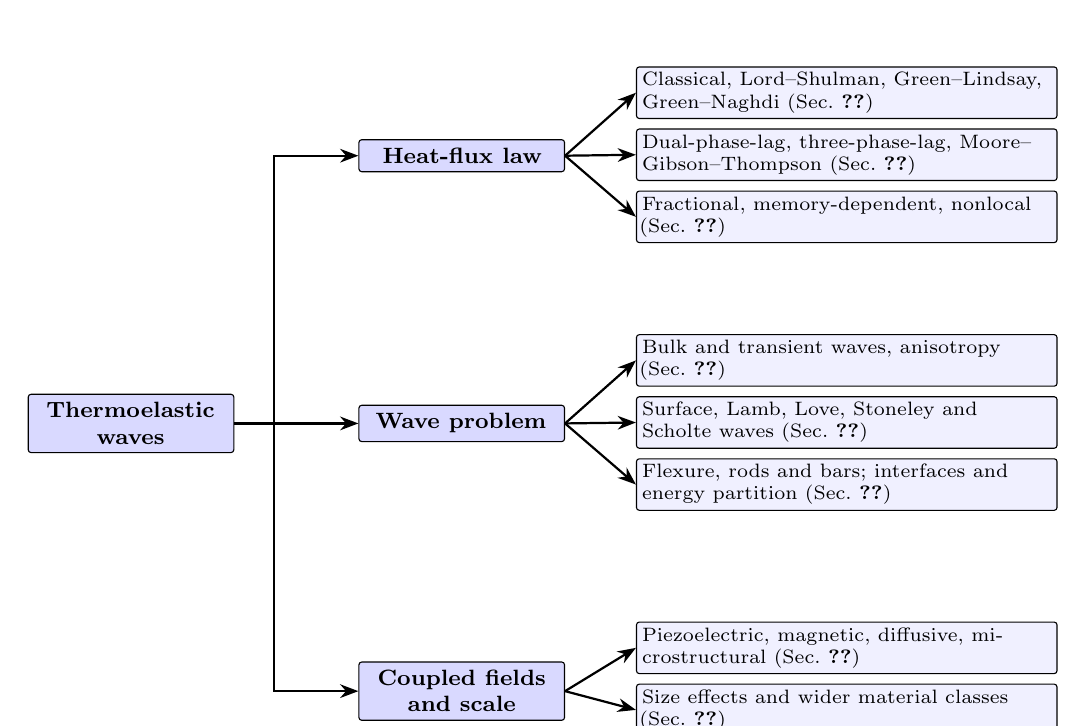
\begin{tikzpicture}[x=1cm,y=1cm,>=Stealth,
  n/.style={draw,rounded corners=1pt,fill=blue!6,font=\scriptsize,align=left,inner sep=2pt,text width=5.2cm},
  h/.style={draw,rounded corners=1pt,fill=blue!15,font=\footnotesize\bfseries,align=center,inner sep=3pt,text width=2.4cm},
  a/.style={->,thick}]
  \node[h] (root) at (0,0) {Thermoelastic waves};
  \node[h] (A) at (4.2,3.4) {Heat-flux law};
  \node[h] (B) at (4.2,0) {Wave problem};
  \node[h] (C) at (4.2,-3.4) {Coupled fields and scale};
  \draw[a] (root.east) -- ++(0.5,0) |- (A.west);
  \draw[a] (root.east) -- ++(0.5,0) |- (B.west);
  \draw[a] (root.east) -- ++(0.5,0) |- (C.west);
  \node[n,right=0.9cm of A,yshift=0.8cm] (A1) {Classical, Lord--Shulman, Green--Lindsay, Green--Naghdi (Sec.~\ref{sec:part_theories})};
  \node[n,below=0.12cm of A1] (A2) {Dual-phase-lag, three-phase-lag, Moore--Gibson--Thompson (Sec.~\ref{sec:part_theories})};
  \node[n,below=0.12cm of A2] (A3) {Fractional, memory-dependent, nonlocal (Sec.~\ref{sec:part_beyond})};
  \draw[a] (A.east) -- (A1.west); \draw[a] (A.east) -- (A2.west); \draw[a] (A.east) -- (A3.west);
  \node[n,right=0.9cm of B,yshift=0.8cm] (B1) {Bulk and transient waves, anisotropy (Sec.~\ref{sec:part_waves})};
  \node[n,below=0.12cm of B1] (B2) {Surface, Lamb, Love, Stoneley and Scholte waves (Sec.~\ref{sec:part_waves})};
  \node[n,below=0.12cm of B2] (B3) {Flexure, rods and bars; interfaces and energy partition (Sec.~\ref{sec:part_waves})};
  \draw[a] (B.east) -- (B1.west); \draw[a] (B.east) -- (B2.west); \draw[a] (B.east) -- (B3.west);
  \node[n,right=0.9cm of C,yshift=0.55cm] (C1) {Piezoelectric, magnetic, diffusive, microstructural (Sec.~\ref{sec:part_fields})};
  \node[n,below=0.12cm of C1] (C2) {Size effects and wider material classes (Sec.~\ref{sec:part_beyond})};
  \draw[a] (C.east) -- (C1.west); \draw[a] (C.east) -- (C2.west);
\end{tikzpicture}
\caption{Classification of the field used to organize this review, with the sections in which each branch is treated.}\label{fig:classification}
\end{figure}


\section{Background}\label{sec:part_foundations}
\demoteopen
\section{Historical development of the theories reviewed}\label{sec:history}
\subsection{A short history}
\paragraph{Origins (1830s--1950s).} Duhamel's memoir of 1837 \citep{Duhamel1837} established the stress--strain--temperature relation that still bears his name (with Neumann's later contribution). The stress depends on strain and on the temperature increment through an expansion coefficient. Dynamic coupling came much later. Biot \citep{Biot1956} showed that the classical thermoelastic equations follow from the thermodynamics of irreversible processes with a Rayleigh-type dissipation function. Achenbach \citep{Achenbach1968} studied the propagation of discontinuities of stress and temperature in a one-dimensional medium with coupled displacement and temperature fields. Dafermos \citep{Dafermos1968} treated the existence and asymptotic stability of solutions of the linear thermoelastic initial-boundary-value problem. Danilovskaya \citep{Danilovskaya1950} solved the thermal shock of an elastic half-space in the uncoupled approximation. Chadwick and Sneddon \citep{ChadwickSneddon1958} analyzed plane waves in the coupled theory, Chadwick's chapter \citep{Chadwick1960} became the standard reference for the dynamical theory. Compact textbook accounts followed \citep{Boley1960,Nowacki1975,Carlson1972}. Three results from that period still organize the subject. In an isotropic solid, shear waves are unaltered by thermal effects; two distinct dilatational waves exist, both dispersed and attenuated \citep{Deresiewicz1957}; and the temperature field obeys a diffusive equation rather than a wave equation. Zener's earlier analysis of thermoelastic internal friction in vibrating reeds \citep{Zener1937} had already found the same relaxation behavior from a different direction.

\paragraph{Finite-speed heat conduction (1940s--1970s).} The conceptual starting point is Cattaneo's 1948 note \citep{Cattaneo1948} and Vernotte's independent discussion \citep{Vernotte1958}. Both add a relaxation term to Fourier's law, which makes the heat equation hyperbolic. The review of Chandrasekharaiah \citep{Chandrasekharaiah1986} summarizes them and records the second-sound experiments mentioned below. Experimental support came from low-temperature solids, in the form of second sound in solid helium and in sodium fluoride \citep{Ackerman1966,Jackson1970}. A kinetic theory of phonon hydrodynamics supplied the physical context in which heat actually propagates as a wave \citep{GuyerKrumhansl1966,GuyerKrumhansl1966II,Chester1963}. Lord and Shulman \citep{Lord1967} then built a heat law of the Cattaneo (Maxwell--Cattaneo) form into a complete thermoelastic theory. Green and Lindsay \citep{Green1972} proposed a different extension, with temperature-rate terms in the constitutive relations whose two coefficients the literature later called relaxation times. Gurtin and Pipkin \citep{GurtinPipkin1968} developed a general theory of heat conduction with finite wave speeds, starting from the same objection to the parabolic equation. Nayfeh and Nemat-Nasser \citep{NayfehNematNasser1971} used the Maxwell-type modified heat law to study plane harmonic waves in unbounded and layered media. The relation of both theories to thermodynamics drew extensive discussion, reviewed in \citep{Chandrasekharaiah1986,Joseph1989,Joseph1990}.

\paragraph{Energy-based theories (1990s).} Green and Naghdi \citep{Green1991,GreenGN1992,Green1993} set out a family of three theories (types I, II, III) on an entropy balance rather than an entropy inequality for the heat flux. The thermal displacement plays the role of a potential. Type II is nondissipative and carries undamped thermal waves; type III contains classical damping as well as thermal waves. Uniqueness and stability theory developed around them \citep{Chandrasekharaiah1996}.

\paragraph{Lagging models (1995--2010).} Tzou \citep{Tzou1995,Tzou1997} separated the heat flux and the temperature gradient by delay times, which gave the dual-phase-lag (DPL) model. Roy Choudhuri \citep{RoyChoudhuri2007} added a third lag, the one associated with the thermal displacement. Both spread quickly, because Taylor expansion of the lag equation gives a differential equation of finite order whose parameters can be fitted to data. Stability and thermodynamic consistency of those truncations have since been studied model by model \citep{Quintanilla2003DPL,Chirita2016,Tibullo2017,vanDerMerwe2021}, with each paper treating its own truncation by its own method.

\paragraph{Nonlocal, fractional and memory-dependent extensions (1970s--present).} Eringen's nonlocal elasticity \citep{Eringen1972,Eringen1983,Eringen2002} and its thermoelastic extension \citep{Eringen1974} predate the generalized heat theories, and they converge with them in micro- and nanosystems. Gradient elasticity \citep{Aifantis1992,Aifantis2003,Askes2006,Askes2011} is the other main enrichment. Fractional calculus entered heat conduction through the Caputo derivative \citep{Caputo1967}, and grew into fractional thermoelasticity \citep{Povstenko2004,Povstenko2007,Povstenko2009,Povstenko2011Cattaneo,Povstenko2016,Sherief2010Fractional,Ezzat2011}. The memory-dependent derivative of Wang and Li \citep{Wang2011,Wang2021} joined it later. Two-temperature theories \citep{ChenGurtin1968,Youssef2006} and their hyperbolic variants \citep{Prasad2020,Alzahrani2020,Bassiouny2020} separate the conductive from the thermodynamic temperature.

\paragraph{Mathematical thermoelasticity of third order (2010s).} The Moore--Gibson--Thompson (MGT) equation comes from the acoustics of a gas with relaxation \citep{MooreGibson1960}. It was studied systematically as an evolution problem \citep{MarchandMcDevittTriggiani2012,LasieckaWang2015MGT,DellOroLasieckaPata2016MGT,DellOroPata2016Viscoelasticity} and then brought into thermoelasticity by Quintanilla \citep{Quintanilla2019,Bazarra2021MGTradial}. The resulting model fits the template of Section~\ref{sec:framework-link}.

\paragraph{Multiphysics and structure (1960s--present).} Micropolar and microcontinuum theories \citep{Eringen1966a,TauchertClausAriman1968,Eringen1999}, materials with voids \citep{Nunziato1979,Cowin1983,Iesan1986}, thermopiezoelectricity \citep{Mindlin1974Thermopiezo,Nowacki1978,Chandrasekharaiah1984}, and thermoelastic diffusion and magneto-thermoelasticity extended the mechanical content, usually with the heat law kept as an independent module. For piezoelectric media, Chandrasekharaiah \citep{Chandrasekharaiah1988} formulated a generalized theory of thermoelasticity that includes the heat flux among the independent constitutive variables. \Cref{fig:timeline} places these developments on one time line.

\begin{figure}[t]\centering
\resizebox{\linewidth}{!}{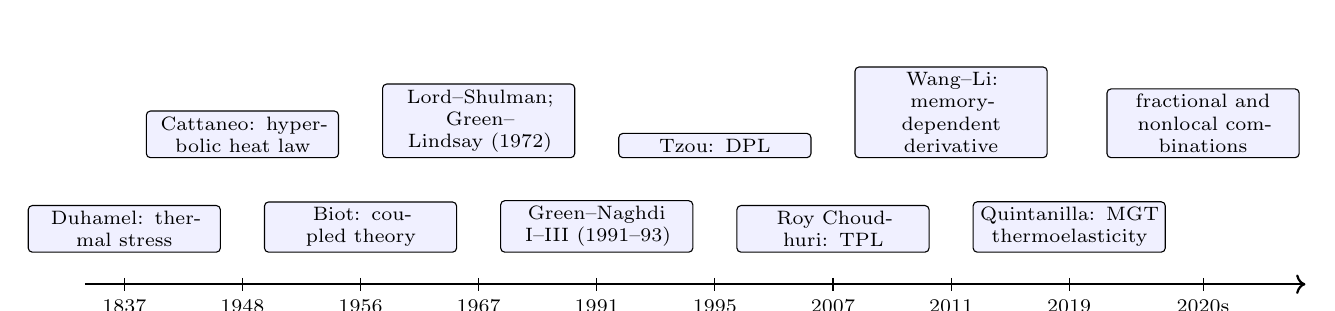
\begin{tikzpicture}[x=1cm,y=1cm,every node/.style={font=\scriptsize},
 ev/.style={draw,rounded corners=1.5pt,fill=blue!6,align=center,inner sep=2pt,text width=2.3cm}]
\draw[->,thick] (0,0)--(15.5,0);
\foreach \x/\l in {0.5/1837,2.0/1948,3.5/1956,5.0/1967,6.5/1991,8.0/1995,9.5/2007,11.0/2011,12.5/2019,14.2/2020s}{\draw (\x,0.08)--(\x,-0.08); \node[below] at (\x,-0.08) {\l};}
\node[ev,above] at (0.5,0.4) {Duhamel: thermal stress};
\node[ev,above] at (2.0,1.6) {Cattaneo: hyperbolic heat law};
\node[ev,above] at (3.5,0.4) {Biot: coupled theory};
\node[ev,above] at (5.0,1.6) {Lord--Shulman; Green--Lindsay (1972)};
\node[ev,above] at (6.5,0.4) {Green--Naghdi I--III (1991--93)};
\node[ev,above] at (8.0,1.6) {Tzou: DPL};
\node[ev,above] at (9.5,0.4) {Roy Choudhuri: TPL};
\node[ev,above] at (11.0,1.6) {Wang--Li: memory-dependent derivative};
\node[ev,above] at (12.5,0.4) {Quintanilla: MGT thermoelasticity};
\node[ev,above] at (14.2,1.6) {fractional and nonlocal combinations};
\end{tikzpicture}}
\caption{Milestones in the theory of thermoelastic waves. Dates are those of the cited original publications (Cattaneo 1948, Vernotte 1958, Biot 1956, Lord--Shulman 1967, Green--Lindsay 1972, Green--Naghdi 1991--1993, Tzou 1995, Roy Choudhuri 2007, Wang--Li 2011, Quintanilla 2019).}\label{fig:timeline}
\end{figure}

\subsection{A map of the contemporary literature}
Three largely independent axes sort the recent literature on wave problems in thermoelastic and multiphysics media: the \emph{heat-flux law}, the \emph{constitutive enrichment} (nonlocal, gradient, microstructural, multiphysics), and the \emph{problem type} (plane waves, surface waves, reflection and transmission, transient response). A typical paper chooses one entry on each axis and computes dispersion curves or response histories. \Cref{tab:streams} lists representative works from the reference list of this review by problem type. The sorting is editorial, and many papers appear in more than one row.

\begin{table}[t]\centering\small
\caption{Representative literature by problem type and constitutive enrichment (selection from the reference list; classification by the titles and stated subjects of the works).}\label{tab:streams}
\begin{tabularx}{\textwidth}{@{}p{3.2cm}X@{}}\toprule
Problem type & Representative works\\\midrule
Plane waves, stability, dispersion & Prasad--Kumar \citep{Prasad2020}; Tiwari--Kumar (nonlocal TPL) \citep{Tiwari2021}; van der Merwe et al. (modal comparison of heat laws) \citep{vanDerMerwe2021}; Sarkar et al.\ (nonlocal type II) \citep{Sarkar2019}.\\
Surface waves & Biswas (porous nonlocal, orthotropic; piezothermoelastic layer) \citep{Biswas2020a,Biswas2020}; Tung (nonlocal piezoelastic Rayleigh) \citep{Tung2019}; Gupta et al.\ (nonlocal piezo-semiconductor Rayleigh wave) \citep{Gupta2024}; Aldandani et al.\ \citep{Aldandani2026}; Ivanov--Savova (energy flux of surface waves) \citep{IvanovSavova1991}.\\
Reflection at free or insulated boundaries & Das et al.\ \citep{Das2008}; Kalkal et al.\ (nonlocal micropolar with rotation) \citep{Kalkal2020}; Singh--Guha (piezothermoelastic fiber-reinforced) \citep{Singh2020b}; Yadav et al.\ \citep{Yadav2023}; Gupta et al.\ \citep{Gupta2024a}; Singh et al.\ (flexoelectric) \citep{Singh2020c}; Jiao et al.\ (flexomagnetic) \citep{Jiao2024}.\\
Interfaces and energy partition & Barak et al.\ \citep{Barak2023,Barak2023IJP,Barak2023JTS,Barak2023MMMS}; Gupta--Kumar \citep{Gupta2023IJNMF,Gupta2023Energy}; Kumar et al.\ \citep{Kumar2023PhysScr,Kumar2019,Kumar2022,Kumar2024,Kumar2024a,Kumar2025,KumarKansal2017,Kumar2018}; Fu--Wei (micropolar imperfect interface) \citep{Fu2013}; Liu et al.\ (graded piezoelectric) \citep{Liu2020}.\\
Transient response, rods, bodies & Singh--Pal \citep{Singh2019,Singh2020a}; Biswas \citep{Biswas2019}; Sur et al.\ \citep{Sur2019,Sur2025}; Bayones et al.\ \citep{Bayones2021}; Li et al.\ (laser pulse, bilayer) \citep{Li2019}; Abouelregal \citep{Abouelregal2023,Abouelregal2020,Abouelregal2020a}; Lata et al.\ \citep{Lata2020}.\\
Damping in resonators & Yang et al.\ (DPL damping in nonlocal nanoplates) \citep{Yang2021}; Kumar et al.\ (couple stress plates) \citep{Kumar2017}.\\
Fractional and memory models & Povstenko \citep{Povstenko2004,Povstenko2009,Povstenko2011Cattaneo,Povstenko2016}; Sherief et al.\ \citep{Sherief2010Fractional}; Ezzat--El-Karamany \citep{Ezzat2011}; Wang--Li \citep{Wang2011,Wang2021,WangLi2025IV}; Yu et al.\ \citep{Yu2024}; Bachher--Sarkar \citep{Bachher2019}.\\
Size effects & Eringen \citep{Eringen1972,Eringen1983}; Aifantis \citep{Aifantis1992}; Askes--Aifantis \citep{Askes2006,Askes2011}; Maranganti--Sharma \citep{Maranganti2006,Maranganti2007}; Lazar--Agiasofitou \citep{Lazar2022}; Zang et al.\ \citep{Zang2014}; Li et al.\ \citep{Li2018}.\\
Variational and uniqueness theory & Marotti de Sciarra \citep{Marotti2013}; Srivastava--Mukhopadhyay \citep{Srivastava2026}; Chandrasekharaiah \citep{Chandrasekharaiah1996}; Chiri\c{t}\u{a} et al.\ \citep{Chirita2016,Tibullo2017}.\\
\bottomrule\end{tabularx}
\end{table}

\subsection{Recurrent observations from the literature}
Four patterns in these streams shape the rest of the review.
\begin{itemize}
\item \textbf{The heat law and the elastic enrichment are treated as independent modules.} Most interface and surface-wave papers combine one of several heat laws with one of several enrichments, so the dispersion relations differ only through $G(s)$ and through the elastic operator. That modularity is what makes a unified treatment possible, and it is also why a limit-checking discipline matters.
\item \textbf{Energy ratios and amplitude ratios dominate the reflection literature.} The interface papers cited above report energy ratios, whose sum must equal one in a lossless setting. A sum different from one is therefore a diagnostic of dissipation, of an error in the flux definition, or of both; Section~\ref{sec:interfaces} discusses this check in detail.
\item \textbf{Parameter values are rarely tied to measurements.} Lags and fractional orders are usually assigned convenient values, so many figures demonstrate a model rather than a material.
\item \textbf{The thermodynamic status of the Taylor-expanded models is delicate.}

\begin{summarybox}[Summary]
The historical line runs Fourier (parabolic) $\to$ Cattaneo/Vernotte (flux relaxation) $\to$ Lord--Shulman $\to$ Green--Lindsay $\to$ Green--Naghdi types I--III $\to$ dual-phase-lag $\to$ three-phase-lag $\to$ Moore--Gibson--Thompson $\to$ fractional and memory-dependent laws. Each step adds one modeling ingredient (relaxation time, second temperature, thermal displacement, lag on temperature gradient, inertia term, memory kernel). Recurrent pitfalls: unmeasured lag parameters, Taylor truncation passed off as exact, mode-flux sums mistaken for energy conservation, GN-III confused with a finite-speed theory.
\end{summarybox} The papers of Chiri\c{t}\u{a} and co-workers \citep{Chirita2016,Tibullo2017} examine thermodynamic compatibility and continuous dependence of the time-differential lag models, and the stability computation reported in Section~\ref{sec:lags} shows how strongly the truncation order matters.
\end{itemize}

\demoteclose
\demoteopen
\section{Thermomechanical foundations}\label{sec:foundations}
This section collects the balance laws, the thermodynamic structure of linear thermoelasticity, the reasons Fourier's law fails for fast processes, and the heat-flux template that organizes the rest of the review. The presentation is self-contained, so later sections can cite equation numbers instead of rederiving them.

\subsection{Balance laws for small disturbances}
Let a body occupy a region $\Omega$ and let $\bu(\bx,t)$ be the displacement from a reference state at uniform temperature $T_0$ and zero stress. For small displacement gradients the strain is $\varepsilon_{ij}=\tfrac12(u_{i,j}+u_{j,i})$. The local forms of the balance of linear momentum and of energy are
\begin{align}
\rho\,\ddot u_i &= \sigma_{ij,j}+\rho f_i, \label{eq:mom}\\
\rho\,\dot e &= \sigma_{ij}\dot\varepsilon_{ij}-q_{i,i}+\rho r, \label{eq:first}
\end{align}
where $\rho$ is the (reference) density, $f_i$ the body force per unit mass, $e$ the specific internal energy, $q_i$ the heat flux and $r$ the heat supply per unit mass. Balance of angular momentum makes the stress symmetric when no couple stresses act. The second law, in the Clausius--Duhem form used by Coleman and Noll \citep{Coleman1963},
\begin{equation}
\rho\,\dot\eta \;\ge\; \frac{\rho r}{T}-\Bigl(\frac{q_i}{T}\Bigr)_{,i}, \label{eq:clausius}
\end{equation}
with specific entropy $\eta$ and absolute temperature $T$, restricts the constitutive relations; Liu \citep{Liu1972} introduced Lagrange multipliers to impose the entropy principle on the constitutive relations, in place of case-by-case manipulation. Eliminating $r$ between \eqref{eq:first} and \eqref{eq:clausius} and introducing the Helmholtz free energy $\psi=e-T\eta$ gives
\begin{equation}
-\rho\bigl(\dot\psi+\eta\dot T\bigr)+\sigma_{ij}\dot\varepsilon_{ij}-\frac{q_i T_{,i}}{T}\;\ge\;0. \label{eq:CDpsi}
\end{equation}
For a material with $\psi=\psi(\varepsilon_{ij},T)$, \eqref{eq:CDpsi} must hold for arbitrary $\dot\varepsilon_{ij}$ and $\dot T$, so the coefficients of those rates vanish,
\begin{equation}
\sigma_{ij}=\rho\,\frac{\partial\psi}{\partial\varepsilon_{ij}},\qquad \eta=-\frac{\partial\psi}{\partial T},\label{eq:coleman}
\end{equation}
and the remaining term gives the \emph{heat-conduction inequality}
\begin{equation}
q_iT_{,i}\;\le\;0.\label{eq:cond-ineq}
\end{equation}
Fourier's law $q_i=-k_{ij}T_{,j}$ with positive-semidefinite $k_{ij}$ satisfies \eqref{eq:cond-ineq} identically, as does any law whose flux is, to leading order, opposed to the temperature gradient. Here lies the difficulty with lagged and relaxed laws (\cref{sec:beyond}).

\subsection{Linear thermoelasticity}
Expand $\rho\psi$ to second order about $(\varepsilon_{ij},T)=(0,T_0)$, with $\theta=T-T_0$:
\begin{equation}
\rho\psi=\tfrac12C_{ijkl}\varepsilon_{ij}\varepsilon_{kl}-\beta_{ij}\varepsilon_{ij}\theta-\frac{\rho c}{2T_0}\theta^2,\label{eq:psi}
\end{equation}
where $C_{ijkl}$ are the isothermal elastic moduli, $\beta_{ij}$ the thermal-stress tensor and $c$ the specific heat at constant strain. The constant and linear terms in $\theta$ are dropped, since they only fix the reference values of the energy and the entropy. Equations~\eqref{eq:coleman} give
\begin{equation}
\sigma_{ij}=C_{ijkl}\varepsilon_{kl}-\beta_{ij}\theta,\qquad \rho\eta=\beta_{ij}\varepsilon_{ij}+\frac{\rho c}{T_0}\theta.\label{eq:stress}
\end{equation}
The first of these is the Duhamel--Neumann relation. For an isotropic solid $C_{ijkl}=\lambda\delta_{ij}\delta_{kl}+\mu(\delta_{ik}\delta_{jl}+\delta_{il}\delta_{jk})$ and $\beta_{ij}=\beta\delta_{ij}$ with $\beta=(3\lambda+2\mu)\alpha_T$, because free thermal expansion $\varepsilon_{ij}=\alpha_T\theta\,\delta_{ij}$ must produce zero stress: $\sigma_{ij}=(3\lambda+2\mu)\alpha_T\theta\,\delta_{ij}-\beta\theta\,\delta_{ij}=0$. The energy balance $\rho T\dot\eta=-q_{i,i}+\rho r$, which is the entropy form of \eqref{eq:first} once the stress power is accounted for by the free energy, linearized about $T_0$ with the second of \eqref{eq:stress}, gives
\begin{equation}
\rho c\,\dot\theta+T_0\,\beta_{ij}\dot\varepsilon_{ij}=-q_{i,i}+\rho r. \label{eq:en}
\end{equation}
Together with \eqref{eq:mom}, \eqref{eq:stress} and a heat-flux law, \eqref{eq:en} closes the system. Each coefficient has a direct physical meaning. The product $\rho c$ is the heat capacity per unit volume at constant strain; $T_0\beta^2/(\rho c)$ is the difference between the adiabatic and isothermal longitudinal moduli,
\begin{equation}
\lambda_{\rm ad}+2\mu_{\rm ad}=\lambda+2\mu+\frac{T_0\beta^2}{\rho c},
\qquad\text{equivalently}\qquad c_{\rm ad}^2=c_1^2\,(1+\varepsilon),\quad \varepsilon=\frac{\beta^2T_0}{\rho^2c\,c_1^2}. \label{eq:adiabatic}
\end{equation}
\cref{tab:materials} gives the coupling parameter $\varepsilon$ and the characteristic frequency $\omega_*=\rho c c_1^2/k$ for representative solids. The coupling is of order $10^{-2}$ for common metals and far smaller for low-expansion materials. The characteristic frequency lies well above the ultrasonic range for bulk solids ($10^{10}$--$10^{13}$ Hz in \cref{tab:materials}). The thermal frequency that matters falls into the megahertz--gigahertz range only when waves are confined to micro-scale structures, where the Zener frequency $f_Z\propto h^{-2}$ takes over (\cref{sec:applications}).
\begin{table}[ht]\centering\small
\caption{Thermoelastic coupling $\varepsilon$ and characteristic frequency $f_*=\omega_*/2\pi$ computed from rounded handbook-type values (300\,K) of density, specific heat, conductivity, expansion coefficient, Young's modulus and Poisson ratio; the reader should replace them by data for the specimen at hand.}\label{tab:materials}
\input{tables/materials.tex}
\end{table}

\subsection{Beyond Fourier's law}\label{sec:beyond}
\paragraph{Why Fourier's law is parabolic.} Inserting $q_i=-kT_{,i}$ in \eqref{eq:en} with constant coefficients and no coupling gives $\rho c\,\dot\theta=k\nabla^2\theta$. The fundamental solution is a Gaussian, nonzero at every distance for every positive time, so the signal speed is unbounded. Because that Gaussian decays so rapidly, the infinite speed has no observable consequence for slow processes. For processes on the time scale of the carrier relaxation it does.

\paragraph{Relaxation of the flux.} A natural modification, due to Cattaneo and Vernotte \citep{Cattaneo1948,Vernotte1958}, lets the flux relax to its Fourier value with relaxation time $\tau_0$:
\begin{equation}
q_i+\tau_0\dot q_i=-k\,\theta_{,i}.\label{eq:cattaneo}
\end{equation}
With \eqref{eq:en} and no coupling, $k\nabla^2\theta=\rho c(\dot\theta+\tau_0\ddot\theta)$, a damped wave equation with front speed $c_T=\sqrt{k/(\rho c\tau_0)}$. In kinetic terms $\tau_0$ is the mean time between momentum-destroying collisions of the heat carriers, and $c_T$ is of the order of the carrier speed divided by $\sqrt3$ in three dimensions. Phonon hydrodynamics admits a different, ``second sound'', regime in which normal (momentum-conserving) collisions dominate \citep{GuyerKrumhansl1966,GuyerKrumhansl1966II,Chester1963}.

\paragraph{Thermodynamic compatibility via extended irreversible thermodynamics.} The Cattaneo law does not follow from \eqref{eq:clausius} with a free energy that depends only on $(\varepsilon_{ij},T)$: the flux itself must enter the state space. Extended irreversible thermodynamics does that \citep{Jou2010,MuellerRuggeri1998,Mueller1967}, with an entropy that depends also on $q_i$. In one dimension, without deformation, take
\begin{equation}
\eta=\eta_{\rm eq}(e)-\frac{\tau_0}{2\rho kT^2}\,q^2,\qquad \rho\dot e=-q_{,x}
\end{equation}
and an entropy flux $q/T$. Then
\begin{equation}
\rho\dot\eta+\Bigl(\frac qT\Bigr)_{,x}=-\frac{q}{kT^2}\bigl(\tau_0\dot q+kT_{,x}\bigr),
\end{equation}
and for the Cattaneo law the bracket equals $-q$, so the entropy production is $q^2/(kT^2)\ge0$. This is the minimal sense in which the relaxed law is thermodynamically admissible: the entropy carries a quadratic correction in the flux. That correction is of second order in the disturbance, which is why the linear theory does not feel it. In lagged models the corresponding entropy functional must be built model by model. For the time-differential three-phase-lag model, thermodynamic principles impose restrictions on the delay times and, in the high-order case, on the conductivities \citep{Chirita2016,Chirita2017}.

\paragraph{Thermal displacement and the Green--Naghdi route.} Green and Naghdi \citep{Green1991,Green1993} take instead an entropy \emph{balance} with an entropy flux, and postulate constitutive relations in terms of the \emph{thermal displacement} $v$, $\dot v=\theta$ (so $v=\int\theta\,\dd t$). The flux $q_i$ may depend on $\theta_{,i}$ and $v_{,i}$; type II ($q_i=-k^*v_{,i}$) conserves energy, and type III adds Fourier dissipation. In wave problems $v$ is the natural field, since $\hat v=\hat\theta/s$.

\paragraph{Green--Lindsay: rates in the stress and entropy.} Green and Lindsay \citep{Green1972} keep a single temperature but let the free energy and the stress depend on $\dot\theta$, so that the entropy and stress relations carry temperature-rate terms. The original paper expresses this through constitutive coefficients and does not name a relaxation time. The relaxation times $\tau_0,\tau_1$ used in this review are the notation of the later literature for those rate coefficients, and the heat flux is taken in its Fourier form, as is usual for the isotropic case. Solutions of the original theory can show discontinuities at wave fronts. A modification with a strain-rate term has been proposed to remove them \citep{Yu2018ModifiedGL}. \cref{sec:hyperbolic} returns to this theory.

\subsection{The heat-flux template}\label{sec:framework-link}
Linear wave problems with constant coefficients depend on the heat-flux law only through its Laplace-domain relation between flux and temperature gradient. The family is therefore defined
\begin{equation}
q_i+\tau_q\,\dot q_i=-k\,\bigl(\theta_{,i}+\tau_T\,\dot\theta_{,i}\bigr)-k^{*}\bigl(v_{,i}+\tau_v\,\dot v_{,i}\bigr),\qquad \dot v=\theta,\label{eq:template}
\end{equation}
After Laplace transformation with zero initial data
\begin{equation}
\hat q_i=-G(s)\,\hat\theta_{,i},\qquad
G(s)=\frac{k\,(1+\tau_Ts)+k^{*}(1+\tau_vs)/s}{1+\tau_qs}.\label{eq:G}
\end{equation}

\begin{figure}[t!]\centering\small
\input{figs_tikz/fig1_template.tex}
\caption{Original schematic; the setting follows \citep{Biot1956}: the heat-flux template couples the flux to temperature gradients through relaxation and lags. Each theory sets some terms to zero.}\label{fig:template}
\end{figure}

\Cref{fig:template} sketches the template. \Cref{tab:param} lists the parameter choices that reproduce the models expressible in the template. Green--Lindsay theory (\cref{sec:gl}) changes the energy and constitutive equations and so is not a row; for fractional and memory-dependent models $G(s)$ keeps the same structure with $s$ replaced by non-integer powers or by kernel transforms (\cref{sec:memory}).

\begin{table}[ht]\centering\small
\caption{Heat-flux theories as parameter choices in the template \eqref{eq:template}. All entries use the energy balance \eqref{eq:en}.}\label{tab:param}
\begin{tabular}{@{}lccccc l@{}}\toprule
Theory & $k$ & $k^*$ & $\tau_q$ & $\tau_T$ & $\tau_v$ & Source\\\midrule
Classical (Fourier) & $k$ & 0 & 0 & 0 & 0 & \citep{Biot1956}\\
Lord--Shulman (Cattaneo) & $k$ & 0 & $\tau_0$ & 0 & 0 & \citep{Lord1967,Cattaneo1948,Vernotte1958}\\
Dual-phase-lag (DPL), 1st order & $k$ & 0 & $\tau_q$ & $\tau_T$ & 0 & \citep{Tzou1995,Tzou1997}\\
Green--Naghdi II & 0 & $k^*$ & 0 & 0 & 0 & \citep{Green1993}\\
Green--Naghdi III & $k$ & $k^*$ & 0 & 0 & 0 & \citep{Green1991}\\
Three-phase-lag (TPL) & $k$ & $k^*$ & $\tau_q$ & $\tau_T$ & $\tau_v$ & \citep{RoyChoudhuri2007}\\
MGT (flux form) & $k$ & $k^*$ & $\tau_q$ & 0 & 0 & \citep{Quintanilla2019}\\\bottomrule
\end{tabular}
\end{table}

\paragraph{Exact reductions and singular limits.} The function $G(s)$ decides which reductions are regular. The following was verified symbolically (reduction check).
\begin{itemize}
\item \textbf{DPL $\to$ Lord--Shulman:} $\tau_T\to0$ with $\tau_q=\tau_0$ fixed and $k^*=0$. Letting $\tau_q\to0$ with $\tau_T$ fixed gives instead $G=k(1+\tau_Ts)$, a Fourier law with a temperature-rate term (Kelvin--Voigt-like conduction), not Cattaneo.
\item \textbf{TPL $\to$ DPL:} $k^*\to0$. For $k^*\ne0$ the function $G(s)\sim k^*/s$ as $s\to0$, so the low-frequency and long-time response changes qualitatively.
\item \textbf{TPL $\to$ classical:} $k^*\to0$ and all three lags $\to0$.
\item \textbf{GN-II:} $k=0$, all lags zero, $G=k^*/s$; \textbf{GN-III:} all lags zero, $G=k+k^*/s$.
\item \textbf{Large-$s$ behavior.} $G(\infty)=0$ for Lord--Shulman (hyperbolic behavior, finite thermal speed $c_T$); $G(\infty)=k\tau_T/\tau_q$ for DPL, which is diffusive again at high frequency with effective conductivity $k\tau_T/\tau_q$.
\item \textbf{Fractional orders:} the endpoint $\alpha\to2$ of the Caputo family is second order in time and is not Fourier's law (\cref{sec:memory}).
\end{itemize}

\subsection{Energy balance and energy flux}\label{sec:energy}
For the Lord--Shulman model without body forces and heat supply, multiply \eqref{eq:mom} by $\dot u_i$ and \eqref{eq:en} by $\theta/T_0$, and use \eqref{eq:cattaneo}:
\begin{equation}
\frac{\partial\mathcal E}{\partial t}+P_{i,i}=-\frac{q_iq_i}{kT_0},\qquad
\mathcal E=\tfrac12\rho\dot u_i\dot u_i+\tfrac12C_{ijkl}\varepsilon_{ij}\varepsilon_{kl}+\frac{\rho c}{2T_0}\theta^2+\frac{\tau_0}{2kT_0}q_iq_i,\label{eq:energy}
\end{equation}
\begin{equation}
P_i=-\sigma_{ij}\dot u_j+\frac{\theta\,q_i}{T_0}.\label{eq:P}
\end{equation}
Here $\mathcal E$ is positive definite, $P_i$ is the flux associated with it, and the right-hand side is the dissipation. This quadratic (availability-type) energy and its flux $P_i$ are what linear wave theory means by ``energy flux''. They differ from the flux $q_i-\sigma_{ij}\dot u_j$ of the \emph{total} internal energy, whose heat-flux part is first order in the disturbance and averages to zero over a period. For the classical theory the same procedure gives \eqref{eq:energy} without the last term in $\mathcal E$. For other members of the template an energy functional exists under parameter conditions that must be stated model by model: for Green--Naghdi type II the functional is conserved; for the first-order DPL and TPL truncations none is constructed here. Stability of the one-dimensional DPL problem was obtained by a spectral argument \citep{Quintanilla2003DPL}. Thermodynamic compatibility and continuous dependence of the time-differential TPL model are treated in \citep{Chirita2016}. \cref{sec:interfaces} uses \eqref{eq:P} for interface energy partition.

\paragraph{The exact total-energy flux, and the reduced form.}
The availability flux \eqref{eq:P} satisfies a dissipation identity, and it is the flux used for the interface energy partition in \cref{sec:interfaces}. There it is the net flux across the interface, and not the sum of per-mode fractions, that is conserved. It is \emph{not} the flux of
total energy, and the difference matters whenever a fixed control volume is meant rather than a material
element. Add the mechanical power balance to the internal-energy balance, convert the material
derivative with mass conservation, and write $\mathcal E_{\mathrm{tot}}=\rho\bigl(\tfrac12\dot\nu_i\dot u_i+e\bigr)$ for the total energy per unit volume. The balances are read here as spatial balances, with $\rho$, $\sigma_{ij}$ and $q_i$ the current density, Cauchy stress and spatial heat flux. They coincide with the referential quantities of the linearized theory used elsewhere in this review only to first order in the disturbance, and the advection term below is of higher order. The result is the identity
\begin{equation}\label{eq:exactflux}
\frac{\partial \mathcal E_{\mathrm{tot}}}{\partial t}
+\frac{\partial}{\partial x_j}\Bigl(q_j-\sigma_{ji}\dot u_i+\mathcal E_{\mathrm{tot}}\dot u_j\Bigr)
=\rho f_i\dot u_i+\rho r ,
\end{equation}
so that with no body force and no heat supply the outward-positive Eulerian flux is
\begin{equation}\label{eq:exactflux-balance}
F_j=q_j-\sigma_{ji}\dot u_i+\mathcal E_{\mathrm{tot}}\dot u_j,
\qquad
\frac{\partial \mathcal E_{\mathrm{tot}}}{\partial t}+\frac{\partial F_j}{\partial x_j}=0 .
\end{equation}
Three contributions appear: conduction $q_j$, stress power $-\sigma_{ji}\dot u_i$, and advection of
total energy $\mathcal E_{\mathrm{tot}}\dot u_j$. The first two alone make the reduced flux
$J_j=q_j-\sigma_{ji}\dot u_i$ that most of the literature uses, and that first-order small-amplitude
wave calculations use; $J_j$ is the first-order reduction of $F_j$ under the stated small-motion
assumptions, not an exact fixed-volume flux.

None of this displaces \eqref{eq:P}. The two objects answer different questions. $P_i$ is the flux tied
to a positive-definite availability functional whose balance carries the dissipation on the right-hand
side. It is also the flux whose net balance across a welded interface is exact in \cref{sec:interfaces}. $F_j$ is the
conserved flux of total energy in a fixed frame. A comparison of one generalized model's energy transport with
another's means something only when it is stated which of the two is being compared. The
reduced notation common in the literature leaves that open.



\begin{summarybox}[Summary]
The balance laws \eqref{eq:mom}\textendash\eqref{eq:en}, the Coleman--Noll relations \eqref{eq:coleman} and the conduction inequality \eqref{eq:cond-ineq} close the system once a heat-flux law is supplied. Fourier's law is parabolic; relaxed and lagged laws give finite-speed thermal waves. The template \eqref{eq:template} reduces to classical, Lord--Shulman (LS), dual-phase-lag (DPL), three-phase-lag (TPL), GN-II/III and MGT by setting its parameters. The endpoint $\tau_q\to0$ with $\tau_T$ fixed, however, is singular (Kelvin--Voigt-like conduction, not Cattaneo). Among these members, only GN-II has a positive-definite energy functional that is conserved exactly in the stated ideal case; the others dissipate it for nonzero coefficients.
\end{summarybox}

\section{Mathematical preliminaries}\label{sec:prelim}

A small set of tools recurs in the later sections. They are collected here with the conventions of this review, so that every statement about branches, damping and dispersion rests on a single definition.

\subsection{Fourier--Laplace conventions}
Fields depend on $\exp[\ii(kx-\omega t)]$ and the Laplace variable is $s=-\ii\omega$, so that $\partial_t\to s$ and $\partial_x\to \ii k$. For a causal response, one that vanishes before the excitation, the transfer functions $G(s)$ and the resulting $k(\omega)$ are analytic in the upper half of the complex $\omega$-plane ($\operatorname{Re}s>0$). Two consequences are used below. The wave number of the uncoupled thermal branch follows from $k^2=-\rho c\,s/G(s)$. The appropriate root is the one whose spatial amplitude does not grow, $\operatorname{Im}k\ge0$, with $\operatorname{Re}k>0$ for propagation in $+x$.

\subsection{Branches and the choice of root}
For the rational heat laws treated in this review, in a linear homogeneous medium, the dispersion relation is a polynomial in $K=k^2$ with coefficients that depend on $s$; for exact delays, fractional powers or hereditary kernels those coefficients are transcendental or multivalued functions of $s$, and the rules below apply with the corresponding branch cuts. Each root $K_j(s)$ therefore gives two wave numbers $\pm\sqrt{K_j}$. Three rules are adopted: (i) for each $K_j$, take the square root with $\operatorname{Im}k\ge0$; (ii) a ``branch'' is a $k(\omega)$ followed continuously in $\omega$, because the labels ``elastic-type'' and ``thermal-type'' mean something only away from hybridization, where roots approach each other; (iii) near hybridization, which in the Lord--Shulman model occurs for $\tau\omega_*\approx1$, tracking by continuity on a sufficiently fine frequency grid is necessary, and selecting the root nearest an expected value fails. Both failures occurred while producing the figures of this review.

\subsection{Spatial and temporal damping}
Loss admits two measures. For real $\omega$ and complex $k$, $Q_x^{-1}=2\operatorname{Im}k/\operatorname{Re}k$; for real $k$ and complex $\omega$, $Q_t^{-1}=2|\operatorname{Im}\omega|/|\operatorname{Re}\omega|$. At weak damping the two are related by the group-to-phase velocity ratio, $Q_t^{-1}\simeq(v_g/v_p)\,Q_x^{-1}$. In the clamped-bar example of \cref{sec:bar} the classical peak $Q_t^{-1}=0.0488$ at $\varepsilon=0.1$ compares with the Debye value $\varepsilon/2=0.05$ of the spatial measure. The difference is a few percent, of the order $\varepsilon$ that the relation predicts. Resonator experiments measure $Q_t$ and wave-propagation experiments $Q_x$, and the two should not be compared without the conversion.

\subsection{Causality and the sum rule}
A causal response obeys the Kramers--Kronig relations, which tie dispersion to loss: a medium with a loss peak must show a change of speed. At weak damping the relation takes the form of a sum rule,
\begin{equation}\label{eq:sumrule}
\int_0^\infty Q_x^{-1}\,d\ln\omega=\pi\,\frac{v_0-v_\infty}{\bar v},
\end{equation}
where $v_0$ and $v_\infty$ are the phase speeds at zero and infinite frequency and $\bar v$ is their mean. For the Debye form $Q^{-1}=\varepsilon x/(1+x^2)$ the left side is $\pi\varepsilon/2$ and the right side is $\pi(\sqrt{1+\varepsilon}-1)\big/\bigl[(\sqrt{1+\varepsilon}+1)/2\bigr]\approx\pi\varepsilon/2$, consistent with the adiabatic and isothermal speeds of \cref{sec:classical}. \Cref{eq:sumrule} was checked numerically on the exact coupled classical dispersion relation (Kramers--Kronig check). At $\varepsilon=0.01$ the integral is $1.562994\times10^{-2}$ against $1.562991\times10^{-2}$ on the right; at $\varepsilon=0.001$ the two sides are $1.570009\times10^{-3}$ and $1.570011\times10^{-3}$. The rule is therefore a practical consistency test on any computed or measured loss curve: a model that predicts a loss peak without a corresponding speed change, or the reverse, either violates causality or has been truncated inconsistently.

\subsection{Support of the solution and finite signal speed}
The Laplace transform of a solution supported in $x\le ct$ decays as $e^{-sx/c}$ for $\operatorname{Re}s\to\infty$. The converse also holds: a transfer function with $k(s)\sim s/c$ at large $s$ implies a front traveling at $c$. That is the origin of the criterion used in \cref{sec:hyperbolic}: finite signal speed requires $sG(s)$ to tend to a finite, non-zero limit. Models with $k_w\sim\sqrt{s}$ at large $s$ (classical, DPL, TPL, GN-III, and the Guyer--Krumhansl law of \cref{sec:kinetic}) have no front, and a transient problem for them has a solution that is nonzero everywhere immediately after the excitation, however small.

\subsection{Complex roots of the delay law}
When $G$ contains an exponential, as in the exact delay law of \cref{sec:delayfid}, $k^2=-\rho c\,s/G(s)$ is an entire function times $s$ and has infinitely many branches. Truncations replace it by a rational function with finitely many roots. Roots of the delay law that the truncation does not contain, and spurious roots that it introduces, plausibly explain why truncated and exact laws differ at $\omega\tau\gtrsim1$, but this has to be checked for each truncation.

\begin{summarybox}[Summary]
The Laplace/Fourier convention ($s=-\ii\omega$, $\Imag k\ge0$ for decay) fixes branch choices once and for all. Damping, attenuation and quality factor are $Q^{-1}=2\Imag k/\Real k$ for spatial problems and $2|\Imag\omega|/\Real\omega$ for temporal problems. Causality follows from analyticity in the upper half-plane; support properties (finite front) are read from the large-$s$ behavior of $G(s)$. The exact delay law has infinitely many branches; truncations keep finitely many and can introduce spurious roots.
\end{summarybox}

\subsection{Admissibility of a heat law}\label{sec:admiss}
A heat law can be wrong in several ways, and the tests are not interchangeable. \emph{Conservation} is built into the balance laws and says nothing about the constitutive law. \emph{Thermodynamic admissibility} asks whether the law is compatible with the second law. For materials with internal state variables the Clausius--Duhem inequality restricts the response functions \citep{ColemanGurtin1967}. For heat conduction with memory it restricts the relaxation functions, not merely the signs of coefficients \citep{ChenNunziato1974}. \emph{Causality} asks that the response vanish before the excitation, which for the transfer function means analyticity for $\operatorname{Re}s>0$. \emph{Stability} asks that no mode grow in time. \emph{Finite speed} is a property of the high-frequency limit and stands independent of the others. A model can pass one test and fail another.

For the template of \cref{sec:foundations} in a linear, homogeneous medium, two necessary conditions follow from the transfer function $G(s)=\bigl[k(1+\tau_Ts)+k^*(1+\tau_vs)/s\bigr]/(1+\tau_qs)$ of the uncoupled thermal mode. Both are derived here and verified with the admissibility check of \cref{app:repro}.

\paragraph{Mean dissipation.} For a harmonic temperature gradient the time-averaged product $-q\,\theta_{,x}$ is proportional to $\operatorname{Re}G(i\omega)$, and
\begin{equation}\label{eq:reG}
\operatorname{Re}G(i\omega)=\frac{k+k^*(\tau_v-\tau_q)+k\,\tau_q\tau_T\,\omega^2}{1+\tau_q^2\omega^2}.
\end{equation}
A heat flux that on average removes entropy-producing gradients, with the entropy flux taken as $q/T_0$, needs $\operatorname{Re}G\ge0$ at every frequency. For $\tau_q,\tau_T\ge0$ this reduces to
\begin{equation}\label{eq:admiss}
k+k^*(\tau_v-\tau_q)\ \ge\ 0 .
\end{equation}
The Green--Naghdi type-II law ($k=0$, all lags zero) gives $\operatorname{Re}G=0$ at every frequency: it is lossless, which agrees with the statement of Green and Naghdi that this theory involves no dissipation of energy and permits harmonic waves without damping \citep{Green1993}.

\paragraph{Temporal stability.} For a real wave number $\kappa$, put $K=\kappa^2$. The modes $e^{st}$ of the uncoupled thermal equation solve
\begin{equation}\label{eq:cubic}
\rho c\,\tau_q s^3+(\rho c+Kk\tau_T)s^2+K(k+k^*\tau_v)s+Kk^*=0 .
\end{equation}
The Routh--Hurwitz conditions for all roots in the open left half-plane are equivalent to
\begin{equation}\label{eq:rh}
\rho c\,\bigl[k+k^*(\tau_v-\tau_q)\bigr]+Kk\tau_T\,(k+k^*\tau_v)>0 ,
\end{equation}
so that for $\tau_T\ge0$ stability at all wave numbers requires the same inequality \eqref{eq:admiss} as the dissipation test. The strict statement applies for $K>0$, $\tau_q>0$ and $k^*>0$. For $k^*=0$ the cubic has a factor $s$ that comes from the thermal-displacement variable ($\dot v=\theta$) and not from the temperature equation, so the test applies to the remaining quadratic factor; $K=0$ is the uniform, conserved mode ($s=0$); and for $\tau_q=0$ the degree drops and the quadratic test replaces the cubic one. Equation~\eqref{eq:rh} was confirmed against the numerically computed roots of \eqref{eq:cubic} for 20\,000 random parameter sets, with no disagreement. \Cref{tab:admiss} applies both tests to the template models.

\begin{table}[ht]\centering\small
\caption{Admissibility of the template models for the uncoupled thermal mode (derived here; $\tau_q,\tau_T,\tau_v\ge0$). ``Finite speed'' refers to the high-frequency limit of the uncoupled mode.}\label{tab:admiss}
\begin{tabularx}{\textwidth}{@{}p{2.3cm}p{3.0cm}p{3.6cm}X@{}}\toprule
Model & Parameter choice & Dissipation and stability & Comment\\\midrule
Fourier & all lags $=0$, $k^*=0$ & $\operatorname{Re}G=k>0$; stable & Infinite speed.\\
Lord--Shulman & $k^*=0$, $\tau_T=0$ & $\operatorname{Re}G=k/(1+\tau_q^2\omega^2)>0$; stable & Finite speed $\sqrt{k/(\rho c\,\tau_q)}$.\\
Dual-phase-lag & $k^*=0$ & $\operatorname{Re}G>0$ for $\tau_T\ge0$; stable & No finite front in the first-order law (diffusive at high frequency).\\
Green--Naghdi II & $k=0$, lags $=0$ & $\operatorname{Re}G=0$; marginal (purely oscillatory) & Lossless, finite speed.\\
Green--Naghdi III & lags $=0$ & $\operatorname{Re}G=k>0$; stable & Diffusive at high frequency, no finite front.\\
Moore--Gibson--Thompson & $\tau_T=\tau_v=0$ & stable iff $k\ge k^*\tau_q$ (marginal at equality) & Finite speed; not admissible if $k^*\tau_q>k$. The inequality is derived here from the uncoupled thermal mode, and Quintanilla \citep{Quintanilla2019} reports that stability of the model depends on the constitutive parameters.\\
Three-phase-lag & general & stable iff \eqref{eq:admiss} (for $\tau_T\ge0$) & Parameters must be chosen within this region.\\
\bottomrule\end{tabularx}
\end{table}

These tests are necessary, not sufficient. A mode-by-mode check says nothing about the coupled problem, about energy-flux postulates other than $q/T_0$, or about well-posedness of initial-boundary-value problems. The entropy flux in the Green--Naghdi theories is a separate quantity, with the heat flux equal to the temperature times that flux. For type II it follows from the free-energy potential rather than from a Fourier law. In linearized type I it agrees with $q/T_0$ to first order \citep{Green1993}. For a law with memory the second law constrains the relaxation functions themselves. The initial values of the energy and heat-flux relaxation functions are non-negative, and the initial slope of the heat-flux relaxation function is non-positive \citep{ChenNunziato1974}. The equilibrium conductivity is non-negative \citep{ChenNunziato1974}. A Kramers--Kronig check of the kind in \cref{sec:prelim} does not establish admissibility. Inequality \eqref{eq:admiss} is also a parameter restriction that fitted values must respect, and reported phase-lag values should be checked against it before they are used as evidence for a model.

\section{Kinetic origin of the hyperbolic and Guyer--Krumhansl laws}\label{sec:kinetic}

The lag models of \cref{sec:lags} are often introduced through their formal structure rather than from a kinetic argument. Their physical meaning comes from the kinetic theory of phonons, and this section summarizes how the two most-used laws arise there. Standard results of phonon hydrodynamics are stated at the level of structure; coefficient values depend on the dispersion model and should be taken from the original derivations.

\subsection{Relaxation-time closure and the Cattaneo law}
Write the linearized phonon Boltzmann equation for the deviation $n'$ from equilibrium with a single relaxation time $\tau_R$ for momentum-destroying (resistive) scattering. Take the first moment, with the energy flux $q$ as the moment variable, and close it at first order by taking the second moment proportional to the temperature gradient:
\begin{equation}\label{eq:cattkin}
\tau_R\,\dot q+q=-k\,\nabla\theta,\qquad k=\tfrac13 c_v v_{\rm g}^2\tau_R ,
\end{equation}
where $v_{\rm g}$ is the phonon group speed. This is the Cattaneo law with $\tau_q=\tau_R$, valid when the closure holds. The closure requires the phonon mean free path to be small compared with the wavelength, so that $\omega\tau_R\ll1$ and $\ell_{\rm mfp}k\ll1$. Beyond that the closure fails, and the finite speed $\sqrt{k/(c_v\tau_R)}=v/\sqrt3$ should not be expected to describe a ballistic front. Two sources treat this regime directly. Chen \citep{Chen2001} derives ballistic--diffusive equations from the Boltzmann equation in the relaxation-time approximation. The distribution function is split into a part that originates at the boundaries and a part that originates inside the domain. The resulting equations are presented as a better approximation than the Fourier law or the Cattaneo equation when the sample size or the pulse duration is comparable to the carrier mean free path or relaxation time. Dreyer and Struchtrup \citep{DreyerStruchtrup1993} review heat-pulse experiments in dielectric solids at low temperature, including the competition of ballistic phonons, second sound and ordinary conduction. Dreyer and Struchtrup explain these experiments within extended thermodynamics of phonons.

\subsection{Normal scattering and the Guyer--Krumhansl law}
If momentum-conserving (normal) collisions with time $\tau_N$ dominate over resistive ones, $\tau_N\ll\tau_R$, the expansion to the next order yields the Guyer--Krumhansl equation
\begin{equation}\label{eq:GKkin}
\tau_R\,\dot q+q=-k\,\nabla\theta+\ell^{2}\bigl(\nabla^{2}q+2\nabla\nabla\!\cdot q\bigr),
\end{equation}
with a length $\ell$ of order $v_{\rm g}\sqrt{\tau_N\tau_R}$ up to a model-dependent numerical factor ($1/5$ in a common Debye-type derivation). In one dimension the bracket becomes $3q_{,xx}$. Together with $c_v\dot\theta=-q_{,x}$ the uncoupled dispersion relation is
\begin{equation}\label{eq:GKdisp}
k_w^{2}=-\,\frac{c_v\,s\,(1+\tau_R s)}{k+3\ell^{2}c_v s},\qquad s=-i\omega .
\end{equation}
Law \cref{eq:GKkin} is not of the form $\hat q=-G(s)\hat\theta_{,x}$ with $G$ independent of $k_w$: the Laplacian term makes the response wavenumber dependent. The Guyer--Krumhansl law therefore lies outside the template of \cref{sec:foundations} and is treated separately in \cref{sec:size}. The practical consequence is that size effects and relaxation effects cannot be separated by choosing different $G(s)$.


\subsection{Dispersion of the Guyer--Krumhansl law}
\Cref{fig:gk} (Guyer--Krumhansl figure) compares the uncoupled thermal branch for the Fourier, Cattaneo and Guyer--Krumhansl laws, in units with $\chi=k/c_v=1$ and $\tau_R=1$. Read the numbers at $\omega\tau_R=0.1,\,1,\,10,\,100$:
\begin{itemize}
\item Fourier: phase speed $0.45,\,1.41,\,4.48,\,14.1$ (in units of $\sqrt{\chi/\tau_R}$), growing as $\sqrt{\omega}$, and attenuation $\operatorname{Im}k_w=0.22,\,0.71,\,2.2,\,7.1$.
\item Cattaneo ($\ell=0$): $0.43,\,0.91,\,1.00,\,1.00$. The speed saturates at $\sqrt{\chi/\tau_R}$ and the attenuation at $1/(2\sqrt{\chi\tau_R})=0.5$.
\item Guyer--Krumhansl with $\ell^2=0.05$: $0.43,\,0.95,\,1.57,\,5.3$ and attenuation $0.22,\,0.53,\,3.9,\,18$; with $\ell^2=0.3$: $0.45,\,1.34,\,4.2,\,13.4$ and attenuation $0.22,\,0.71,\,2.3,\,7.4$.
\end{itemize}
At low frequency the three laws coincide with diffusion. At high frequency the Cattaneo law approaches a finite front, whereas the Guyer--Krumhansl law returns to diffusive behavior: from \cref{eq:GKdisp}, $k_w^2\to i\omega\tau_R/(3\ell^2)$ for $\omega\to\infty$, so both $\operatorname{Re}k_w$ and $\operatorname{Im}k_w$ grow as $\sqrt{\omega}$ and the phase speed grows as $\sqrt{6\ell^2\omega/\tau_R}$ (confirmed numerically to $0.2\%$). The linear Guyer--Krumhansl law therefore has no finite signal speed in this uncoupled form. Its role is to represent nonlocal (Knudsen-type) corrections at intermediate frequencies, not to enforce a front.

\begin{figure}[t]
\centering
\includegraphics[width=\linewidth]{figs/fig_gk.pdf}
\caption{Thermal branch for Fourier, Cattaneo and Guyer--Krumhansl laws ($\chi=\tau_R=1$): (a) phase speed, (b) attenuation. The dispersion relation is \cref{eq:GKdisp}.}
\label{fig:gk}
\end{figure}
\subsection{What this means for model choice}
Three consequences follow. (i) A lag law states how the flux relaxes; if the heat-carrier mean free path is comparable to the sample, the Guyer--Krumhansl structure or a full kinetic model is the physical starting point. (ii) Parameters $\tau_q$, $\tau_T$ obtained by fitting a lag law to transient data are effective and need not equal a microscopic relaxation time. (iii) A lag law with $\tau_q$ of the order of $10^{-12}$\,s describes phonon relaxation only if a closure of the type above holds at the wavelengths and frequencies of interest.


\begin{summarybox}[Summary]
The kinetic closure gives the Guyer--Krumhansl equation, in which momentum-conserving normal collisions produce a spatial nonlocality of the flux. A lag law is an effective closure, not a microscopic statement: fitted $\tau_q,\tau_T$ need not equal microscopic relaxation times. When the phonon mean free path is comparable to the sample size, kinetic/GK or a full Boltzmann treatment is the physical starting point rather than a pure lag law.
\end{summarybox}

\section{Effective modulus, causality and Kramers--Kronig relations}\label{sec:modulus}
A wave measurement does not return $k(\omega)$ for a heat law. It returns a complex wavenumber that the experimenter reads as a frequency-dependent modulus. That reading is made explicit for the one-dimensional coupled problem, and what causality does and does not imply is stated.

\subsection{The effective modulus is the root of a quadratic}
Define $m(s)=\omega^2/K=-s^2/K$, the squared complex phase speed of the elastic-type branch ($K=k^2$). Substituting $K=-s^2/m$ in \eqref{eq:disp}, with $R=\rho c$ the volumetric heat capacity and $\beta^2T_0$ the coupling, and dividing by $s^3$ gives
\begin{equation}
\rho R\,m^2-\bigl[\rho R\,c_1^2+\rho\,G(s)\,s+\beta^2T_0\bigr]\,m+\rho c_1^2\,G(s)\,s=0 .\label{eq:mquad}
\end{equation}
The effective longitudinal modulus is $M(s)=\rho\,m(s)$, with $m$ the root that tends to $c_1^2$ for $\beta\to0$. Equation \eqref{eq:mquad} contains the heat law only through the product $G(s)\,s$, which is the statement of \cref{sec:identify} in a different form. It is equivalent to \eqref{eq:disp}, and was checked against the numerical roots of the latter for the classical, Lord--Shulman, dual-phase-lag, Green--Naghdi III and Moore--Gibson--Thompson parameter sets (modulus check, agreement to $10^{-10}$).

Three limits follow directly.
\begin{itemize}
\item \emph{Weak coupling.} To first order in $\beta^2T_0$, $m=c_1^2+\beta^2T_0\,c_1^2\big/\bigl[\rho\,(R c_1^2-G s)\bigr]$. For Fourier conduction ($G=k$) this is a single Debye term, $m=c_1^2\bigl[1+\varepsilon/(1+\ii\omega/\omega_*)\bigr]$, the weak-coupling form behind the loss peak of \cref{sec:classical}.
\item \emph{Fourier, exact.} Because $G\,s\to0$ as $s\to0$ and $G\,s\to\infty$ as $s\to\infty$, the elastic-type root tends to the adiabatic value $c_1^2+\beta^2T_0/(\rho R)$ at low frequency and to $c_1^2$ at high frequency, as \cref{sec:classical} states.
\item \emph{Lord--Shulman, high frequency.} With $G\,s\to k/\tau_0$ the two roots of \eqref{eq:mquad} are those of the front relation \eqref{eq:fronts} with $\tau^\dagger=\tau_0$ (verified numerically in the same computation), so the finite thermal front enters the modulus as a finite high-frequency limit.
\end{itemize}
A standard linear solid has a modulus that is a rational function of $s$; $M(s)$ here is an \emph{algebraic} function, a root of a quadratic, with branch points where the discriminant of \eqref{eq:mquad} vanishes. The single Debye form is therefore a weak-coupling approximation, not the exact thermoelastic modulus.

\subsection{What causality implies}
The response of the bar to a force applied at $t=0$ vanishes for $t<0$ if the transfer function is analytic for $\operatorname{Re}s>0$. For the elastic-type root this requires that the discriminant of \eqref{eq:mquad} has no zero there, and that the admissibility conditions of \cref{sec:admiss} hold so that $G$ itself is regular. The first condition was checked on a grid of $60\times201$ points in $0.001\le\operatorname{Re}s\le100$, $|\operatorname{Im}s|\le50$ for the five parameter sets above, and no zero of the discriminant was found. The smallest normalized value exceeded $10^{-6}$. That is a numerical test on a bounded region, not a proof. Where analyticity holds, the real and imaginary parts of $M$ are related by the Kramers--Kronig integrals, and the loss integrates to the dispersion step of the sum rule \eqref{eq:sumrule}, with $c_0,c_\infty$ in the place of $v_0,v_\infty$ and $\bar c$ the mean of the two speeds. The relation is confirmed for the classical coupled wave (Kramers--Kronig check, deviation below $10^{-5}$). The sum rule was checked for the classical model only; for the other heat laws it should hold under the same analyticity condition, but it has not been verified here.

\paragraph{Consequence for fitting.} Analyticity makes a measured attenuation spectrum and a measured velocity spectrum dependent on each other. A lag model fitted separately to the two, with different parameters resulting, is inconsistent with a causal linear response, unless the data are noisy. \Cref{sec:identify} shows which parameter combinations the pair can determine at all.

\demoteclose

\section{The theories as parameter choices of one template}\label{sec:part_theories}
\demoteopen
\section{Classical coupled thermoelasticity}\label{sec:classical}
\subsection{Field equations}
For an isotropic solid with Fourier conduction $q_i=-k\theta_{,i}$, \eqref{eq:mom}, \eqref{eq:stress} and \eqref{eq:en} give the Navier-type system
\begin{align}
\rho\ddot{\bu}&=\mu\nabla^2\bu+(\lambda+\mu)\nabla(\nabla\!\cdot\!\bu)-\beta\nabla\theta+\rho\bm f,\label{eq:navier}\\
\rho c\,\dot\theta&=k\nabla^2\theta-T_0\beta\,\nabla\!\cdot\!\dot{\bu}+\rho r.\label{eq:heateq}
\end{align}
The two coupling terms carry the whole thermodynamic content: the thermal body force $-\beta\nabla\theta$ in \eqref{eq:navier} and the dilatation heating $-T_0\beta\nabla\!\cdot\!\dot{\bu}$ in \eqref{eq:heateq}. Their product, $T_0\beta^2$, is what appears in the single coupling constant $\varepsilon$ of \eqref{eq:adiabatic}, and the reciprocal structure, the same $\beta$ in both terms, follows from the existence of the free energy \eqref{eq:psi}. A sign or factor error in either term breaks that reciprocity and is a common source of unphysical results. The dispersion checks of \cref{app:disp} detect it by comparing the branches symbolically with the field equations.

\paragraph{Helmholtz decomposition.} Writing $\bu=\nabla\phi+\nabla\times\bm\psi$ with $\nabla\!\cdot\!\bm\psi=0$ decouples the problem in an unbounded isotropic body:
\begin{equation}
\rho\ddot\phi=(\lambda+2\mu)\nabla^2\phi-\beta\theta,\qquad
\rho c\dot\theta=k\nabla^2\theta-T_0\beta\nabla^2\dot\phi,\qquad
\rho\ddot{\bm\psi}=\mu\nabla^2\bm\psi.\label{eq:helm}
\end{equation}
The shear potential $\bm\psi$ obeys an uncoupled wave equation with speed $c_2=\sqrt{\mu/\rho}$: in an unbounded isotropic medium, thermoelastic coupling neither attenuates nor disperses transverse waves. Only the dilatational potential couples to temperature. At boundaries and interfaces the boundary conditions couple shear and dilatational motion again, which is why surface waves and reflected shear waves feel the thermal coupling (Sections~\ref{sec:surface} and~\ref{sec:interfaces}).

\Cref{fig:classical-coup} summarizes the coupling structure.

\begin{figure}[t!]\centering\small
\input{figs_tikz/fig2_classical.tex}
\caption{Original schematic; the setting follows \citep{Biot1956}: classical coupled thermoelasticity -- mechanical and thermal fields are linked by the thermal body force and dilatation heating, the two terms sharing $\beta$.}\label{fig:classical-coup}
\end{figure}

\subsection{Uniqueness and energy}
Multiply \eqref{eq:navier} by $\dot u_i$ and \eqref{eq:heateq} by $\theta/T_0$, then integrate. The result is the energy identity \eqref{eq:energy} without the flux-relaxation term, with dissipation $\int k|\nabla\theta|^2/T_0\,\dd V\ge0$. Two consequences follow. Solutions of the initial--boundary value problem are unique under standard boundary conditions, that is, Dirichlet, Neumann or Robin conditions on each of the mechanical and thermal parts. They depend continuously on the data. Variational formulations and reciprocity theorems are available \citep{Carlson1972,Nowacki1975}, and mixed variational formulations exist for the Green--Naghdi type-II model \citep{Marotti2013}. For the generalized theories these identities are where well-posedness proofs begin \citep{Chandrasekharaiah1996,Quintanilla2019}.

\subsection{Longitudinal plane waves}\label{sec:longitudinal}
For one-dimensional dilatational motion, $\bu=u(x,t)\bm e_x$, equations \eqref{eq:navier}--\eqref{eq:heateq} reduce to
\begin{equation}
\rho\ddot u=(\lambda+2\mu)u_{,xx}-\beta\theta_{,x},\qquad \rho c\,\dot\theta+T_0\beta\,\dot u_{,x}=-q_{,x}.\label{eq:1d}
\end{equation}
Introduce $\hat q=-G(s)\hat\theta_{,x}$, so that $G=k$ for the classical theory, and seek solutions $\propto\exp[\ii(kx-\omega t)]$. The characteristic equation is quadratic in $K=k^2$:
\begin{equation}
\bigl(\rho c_1^2K-\rho\omega^2\bigr)\bigl(s\rho c+G(s)K\bigr)+\beta^2T_0\,s\,K=0,\qquad s=-\ii\omega. \label{eq:disp}
\end{equation}
Equation~\eqref{eq:disp} holds for every member of the template of \cref{sec:framework-link}; \cref{app:disp} gives a derivation and the symbolic check against the field equations. Two branches result: an \emph{elastic-type} branch with $k\approx\omega/c_1$ at weak coupling, and a \emph{thermal-type} branch with $k^2\approx-s\rho c/G(s)$. The branches are called types rather than ``waves'', because the classical thermal branch is a diffusive wave with $\Real k=\Imag k$, which attenuates by a factor $e^{-2\pi}$ per wavelength.

\paragraph{Weak-coupling expansion.} Let $x=\omega/\omega_*$ with $\omega_*=\rho c c_1^2/k$. For $\varepsilon\ll1$ and $G=k$, set $K=\omega^2/c_1^2+\delta K$ in \eqref{eq:disp}. To first order in $\varepsilon$,
\begin{equation}
c_1^2K=\omega^2\Bigl[1+\varepsilon\,\frac{-1+\ii x}{1+x^2}\Bigr]\;\Longrightarrow\;
v_p\simeq c_1\Bigl[1+\frac{\varepsilon}{2(1+x^2)}\Bigr],\qquad
Q^{-1}\equiv\frac{2\Imag k}{\Real k}\simeq\varepsilon\,\frac{x}{1+x^2}. \label{eq:debye}
\end{equation}
The phase speed interpolates between the adiabatic value $c_1(1+\varepsilon/2)\simeq c_1\sqrt{1+\varepsilon}$ at low frequency and the isothermal speed $c_1$ at high frequency, and the inverse quality factor $Q^{-1}$ takes the Debye form, with a maximum $\varepsilon/2$ at $\omega=\omega_*$. In the language of anelasticity the relaxation strength is $\varepsilon$ and the relaxation time is $1/\omega_*$. This is Zener's thermoelastic relaxation \citep{Zener1937}, derived here for a plane compressional wave rather than for a vibrating reed. The limits run in the opposite order to what one may first expect. The classical theory is \emph{adiabatic} at low frequency and \emph{isothermal} at high frequency, because conduction over a wavelength is efficient when the wavelength is short ($\alpha k^2\gg\omega$) and negligible when it is long. The Debye form \eqref{eq:debye} was confirmed against the exact roots of \eqref{eq:disp}: for $\varepsilon=10^{-3}$ the exact value of $Q^{-1}/\varepsilon$ at $\omega=\omega_*$ is $0.49999984$ against the predicted $0.5$ (Zener-damping figure).

\begin{figure}[t]\centering
\includegraphics[width=\textwidth]{figs/fig_dispersion.pdf}
\caption{Phase speed (left) and attenuation (right) of the elastic-type (top) and thermal-type (bottom) branches for the classical, Lord--Shulman and dual-phase-lag models. Parameters: $\varepsilon=0.1$ (larger than for metals so that dispersion is visible), $\tau_0=\tau_q=0.25/\omega_*$ giving $c_T=2c_1$, and $\tau_T=\tau_q/2$ for DPL (a stable choice for the first-order model, see \cref{sec:lags}). Dotted lines: isothermal speed $c_1$, adiabatic speed $c_1\sqrt{1+\varepsilon}$, thermal speed $c_T$. Branches are followed by continuity in frequency.}\label{fig:disp}
\end{figure}

\subsection{Thermoelastic damping}\label{sec:ted}
\Cref{fig:zener}(a) compares the exact classical $Q^{-1}$ with the Debye form for two couplings. The weak-coupling formula is accurate to within a few percent already at $\varepsilon=0.02$, and to leading order the curve shape does not depend on $\varepsilon$. Panel (b) shows the effect of the heat-flux law at the larger coupling $\varepsilon=0.1$. All three models share the low-frequency rise $Q^{-1}\propto\omega$ and the maximum near $\omega_*$. The generalized laws raise the maximum and lift the high-frequency tail, by a factor that depends on $\omega\tau_q$ only once that product approaches order one. The relevant parameter is $\omega_*\tau_q$. For the metals of \cref{tab:materials}, $\omega_*\sim10^{11}$--$10^{12}$\,rad/s, a lag time of order a picosecond therefore puts the product near order one at the \emph{bulk} damping peak, and the heat law then matters. That peak lies at tens of gigahertz and is reached only in very high-frequency experiments. In micro- and nano-resonators the relevant relaxation frequency is set by the structure size rather than by $\omega_*$ (see below) and lies far below $1/\tau_q$, where Zener's classical formula suffices. Lagged corrections matter instead for ultra-high-frequency nanostructures (\cref{sec:applications}).
\begin{figure}[t]\centering
\includegraphics[width=\textwidth]{figs/fig_zener.pdf}
\caption{Thermoelastic damping of the elastic-type branch, $Q^{-1}=2\Imag k/\Real k$ against frequency. (a) Classical theory for two couplings ($\varepsilon=0.02$ and $0.1$), normalized by $\varepsilon$, compared with the weak-coupling Debye form \eqref{eq:debye}. (b) Effect of the heat law at $\varepsilon=0.1$, with $\tau_q=0.25/\omega_*$ and DPL $\tau_T=\tau_q/2$.}\label{fig:zener}
\end{figure}

\paragraph{Relation to flexural damping.} In a thin beam of thickness $h$ vibrating in flexure the temperature varies across the thickness with a thermal relaxation time $\tau_Z\simeq h^2/(\pi^2\alpha)$ (Zener). The damping then has the same Debye form with $\omega_*$ replaced by $1/\tau_Z$ and the relaxation strength $\Delta=E\alpha_T^2T_0/(\rho c)$, with Young's modulus $E$ \citep{Zener1937}. Lifshitz and Roukes \citep{Lifshitz2000} derived the corresponding exact expression for beams and discussed its use for micro- and nano-mechanical resonators. For a silicon beam one micrometer thick, $\alpha\approx9\times10^{-5}\,\mathrm{m^2/s}$ gives a relaxation frequency of order $10^8$ Hz, inside the range of present-day resonators. Generalized and nonlocal corrections to this classical result have been studied for nanoplates, with nonlocal elasticity and dual-phase-lag conduction \citep{Yang2021}, and for plate resonators \citep{Kumar2017}.

\subsection{Anisotropy and other classical extensions}
In anisotropic media the field equations keep their form with $C_{ijkl}$, $\beta_{ij}$ and $k_{ij}$; Dhaliwal and Sherief extended the generalized theory to anisotropic media \citep{Dhaliwal1980}. The coupled problem no longer separates into shear and dilatational parts, but quasi-longitudinal, quasi-shear and thermal branches exist. Along symmetric directions the one-dimensional analysis above applies with the appropriate effective moduli. For orthotropic, transversely isotropic and piezoelectric crystals the Stroh formalism \citep{Stroh1958,Stroh1962} gives a systematic route to surface waves.

\subsection{What the classical theory cannot describe}
Three predictions of the classical theory conflict with finite-speed heat transport: the instantaneous thermal signal, the unbounded thermal phase speed (\Cref{fig:disp}c, black curve), and the monotonic growth of thermal attenuation with frequency. How much these matter depends on the time scale $\tau_q$ of the heat carriers and on the dimension of the structure; \cref{sec:synthesis} gives the criteria.

\begin{summarybox}[Summary]
Classical coupled thermoelasticity links mechanics and heat through the shared coefficient $\beta$ in \eqref{eq:navier}\textendash\eqref{eq:heateq}. Shear waves are unaffected; only dilatational motion couples to temperature. The theory is parabolic: infinite thermal signal speed, diffusive thermal branch. Thermoelastic damping follows Zener's Debye form with peak $\varepsilon/2$ at $\omega=\omega_*$, adiabatic at low frequency and isothermal at high frequency.
\end{summarybox}

\section{Hyperbolic theories: LS, GL and GN}\label{sec:hyperbolic}
\subsection{A common dispersion equation}
For plane longitudinal motion the three classical generalized theories fit into one equation. Let $\tau_0$ denote the flux relaxation time (Lord--Shulman) or the thermal relaxation time (Green--Lindsay, in the notation of the later literature). Let $\tau^\dagger$ be the lag that multiplies the thermal-stress and dilatation coupling. Eliminating $\hat u$ and $\hat\theta$ gives
\begin{equation}
\bigl(\rho c_1^2K+\rho s^2\bigr)\Bigl(s\rho c\,(1+\tau_0s)+kK\Bigr)+\beta^2T_0\,s\,K\,(1+\tau^\dagger s)=0,\label{eq:unified}
\end{equation}
with $\tau^\dagger=0$ and $\tau_0=0$ for the classical theory, $\tau^\dagger=\tau_0$ for Lord--Shulman (this is \eqref{eq:disp} multiplied by $1+\tau_0s$), and $\tau^\dagger=\tau_1$, the second relaxation time, for Green--Lindsay. The unified form of Dhaliwal and Sherief \citep{Dhaliwal1980} makes the same point at the level of the field equations. The theories differ in which of the two coupling terms carries a time-derivative correction.

\subsection{Lord--Shulman theory}\label{sec:ls}
The Lord--Shulman (LS) theory joins Cattaneo's law \eqref{eq:cattaneo} to the energy balance \eqref{eq:en}. Eliminating the flux gives the temperature equation
\begin{equation}
k\nabla^2\theta=(1+\tau_0\partial_t)\bigl(\rho c\,\dot\theta+T_0\beta\,\dot\varepsilon_{kk}\bigr)-(1+\tau_0\partial_t)\rho r, \label{eq:LS}
\end{equation}
so the lagged derivative acts on \emph{both} the heat-capacity term and the dilatation-coupling term. The second of these is a modeling consequence of applying the Cattaneo law to the total heat flux, and it produces the difference from the Green--Lindsay equations.

\paragraph{Wave fronts.} Take $\omega\to\infty$ in \eqref{eq:unified}. The leading terms in $s$ give, with $c_T^2=k/(\rho c\tau_0)$ and $\varepsilon=\beta^2T_0/(\rho^2cc_1^2)$,
\begin{equation}
c_{\rm f}^4-c_{\rm f}^2\bigl[c_1^2(1+\varepsilon\,\tau^\dagger/\tau_0)+c_T^2\bigr]+c_1^2c_T^2=0, \label{eq:fronts}
\end{equation}
whose two roots $c_{\rm f}$ are the speeds of the two wave fronts, one elastic-type and one thermal-type, with $v_{\rm e}<v_{\rm t}$ when $c_T>c_1$ (the labels exchange for $c_T<c_1$). For LS, $\tau^\dagger=\tau_0$ and the equation is the standard high-frequency front equation of the theory; for GL it is \eqref{eq:fronts} with the factor $\tau_1/\tau_0$. The front equation \eqref{eq:fronts} was verified numerically against the roots of \eqref{eq:unified} at $\omega/\omega_*=2\times10^3$ for both theories (front-speed check). With $\varepsilon=0.1$ and $\tau_0=0.25/\omega_*$ ($c_T=2c_1$) the LS fronts are $0.9839\,c_1$ and $2.0327\,c_1$. With $\tau_1=0.5/\omega_*$ (admissible, since $\tau_1\ge\tau_0$, and giving $\tau_1/\tau_0=2$) the GL fronts are $0.9689\,c_1$ and $2.0643\,c_1$, in agreement with \eqref{eq:fronts} to four digits. Two features deserve recording.
\begin{enumerate}
\item The elastic front speed is \emph{not} the isothermal speed $c_1$, nor the adiabatic speed. Interaction with the thermal front displaces it, and the two speeds repel one another: their product is $c_1c_T$ and the sum of their squares is $c_1^2(1+\varepsilon\,\tau^\dagger/\tau_0)+c_T^2$, that is $c_1^2(1+\varepsilon)+c_T^2$ for LS. For LS, when $c_T=c_1$ the degeneracy is lifted by an amount proportional to $\sqrt\varepsilon$, $v^2=c_1^2[2+\varepsilon\pm\sqrt{\varepsilon(4+\varepsilon)}]/2\approx c_1^2(1\pm\sqrt\varepsilon)$.
\item The leading front speeds depend only on the high-frequency terms, so they are independent of $k$ except through $c_T$.
\end{enumerate}

The two fronts are sketched in \cref{fig:fronts}.

\begin{figure}[t!]\centering\small
\input{figs_tikz/fig3_fronts.tex}
\caption{Original schematic; the setting follows \citep{Lord1967}: two wave fronts in hyperbolic thermoelasticity -- elastic-type and thermal-type fronts repel in speed; the thermal front carries a damped tail.}\label{fig:fronts}
\end{figure}

\paragraph{Discontinuities and well-posedness.} The system is hyperbolic, so initial data with a jump produce solutions whose jumps travel along the fronts and decay exponentially along the propagation path. The heat-pulse problem of \cref{sec:transient} shows this. The system is well posed for $\tau_0>0$, and energy decays in bounded bodies under standard boundary conditions by the energy identity \eqref{eq:energy}. Existence of generalized solutions was established for one relaxation time by \citep{Bem1982} and for two by \citep{Bem1983}, and domain-of-influence results appear in \citep{Ignaczak1980}. The thermodynamic foundation via the Clausius--Duhem inequality is due to \citep{GurtinWilliams1966}.

\paragraph{Interpretation.} Two modeling questions matter: the physical size of $\tau_0$, and whether Cattaneo's law with a single exponential relaxation describes the frequency range of interest. Joseph and Preziosi \citep{Joseph1989,Joseph1990} review the evidence for and against. Large relaxation times have been reported for nonhomogeneous materials \citep{Kaminski1990,Mitra1995}, though the interpretation of such measurements is debated. For solids the strongest evidence of wave-like heat propagation remains second sound at cryogenic temperatures \citep{Ackerman1966,Jackson1970}. There the governing regime is the Guyer--Krumhansl hydrodynamic one \citep{GuyerKrumhansl1966II} rather than the simple Cattaneo law.

\subsection{Green--Lindsay theory}\label{sec:gl}
The Green--Lindsay (GL) theory \citep{Green1972} has the constitutive relations
\begin{equation}
\sigma_{ij}=C_{ijkl}\varepsilon_{kl}-\beta_{ij}\bigl(\theta+\tau_1\dot\theta\bigr),\qquad
k\theta_{,ii}=\rho c\bigl(\dot\theta+\tau_0\ddot\theta\bigr)+T_0\beta_{ij}\dot\varepsilon_{ij},\label{eq:GL}
\end{equation}
with $\tau_1\ge\tau_0>0$. In the notation of Green and Lindsay \citep{Green1972}, $\tau_1$ is the coefficient $\alpha$ of $\dot\theta$ in the stress relation, and $\tau_0=h/d$ is the ratio of the coefficients of $\ddot\theta$ and $\dot\theta$ in the energy equation. Their restrictions $d\alpha-h\ge0$, $h>0$ (Eqs.~(4.14) and~(4.16) of that paper) give the ordering stated. Heat conduction is Fourier's here, so the theory does not fit the flux template \eqref{eq:template}: the finite thermal speed comes from the inertia term $\tau_0\ddot\theta$ instead. Substitution in plane waves gives \eqref{eq:unified} with $\tau^\dagger=\tau_1$. Three differences from LS matter. First, the thermal equation is not of Cattaneo type, so its relation to kinetic arguments is less direct. Second, the entropy depends on the temperature rate, which puts a thermal-displacement-like quantity into the constitutive structure and makes care necessary in reading $\tau_0$ and $\tau_1$ as independent material constants. Third, solutions of the original theory can contain discontinuities at the wave fronts, and a modification with a strain-rate term was proposed to remove them \citep{Yu2018ModifiedGL}. Wave fronts follow \eqref{eq:fronts} with $\tau^\dagger=\tau_1$, and one consequence distinguishes GL from LS. At the wave fronts the coupling is stronger than in LS by the factor $\tau_1/\tau_0\ge1$. The temperature-rate term in the stress carries $\tau_1$, the thermal inertia carries $\tau_0$, and the strain-rate coupling in the energy equation carries no relaxation time.

\subsection{Green--Naghdi types I, II and III}\label{sec:gn}
The Green--Naghdi (GN) theories \citep{Green1991,GreenGN1992,Green1993} postulate an entropy balance with the thermal displacement $v$ ($\dot v=\theta$) as a primary field. In the template the three types are
\begin{equation}
\text{I: }\ q_i=-k\theta_{,i};\qquad
\text{II: }\ q_i=-k^*v_{,i};\qquad
\text{III: }\ q_i=-k\theta_{,i}-k^*v_{,i},
\end{equation}
with $G=k$, $k^*/s$ and $k+k^*/s$, respectively. Their uncoupled thermal equations are, with $\rho c=1$ for brevity,
\begin{equation}
\text{II: }\ \ddot\theta=c_*^2\nabla^2\theta,\quad c_*^2=k^*/\rho c;\qquad
\text{III: }\ \ddot\theta=c_*^2\nabla^2\theta+\alpha\nabla^2\dot\theta.
\end{equation}
\paragraph{Type II.} Thermal disturbances propagate as undamped waves of speed $c_*$, and with coupling the two fronts satisfy \eqref{eq:fronts} with $c_T\to c_*$ and $\tau^\dagger/\tau_0\to1$. The relation is \emph{exact at every frequency}, not merely asymptotically: the roots of the quadratic \eqref{eq:disp} with $G=k^*/s$ are non-dispersive, with $v^4-v^2[c_1^2(1+\varepsilon)+c_*^2]+c_1^2c_*^2=0$ at every $\omega$. This was confirmed numerically for $\varepsilon=0.1$ and $c_*=c_1$: the exact speeds $0.854309c_1$ and $1.170537c_1$ are the same at $\omega/\omega_*=0.5$, $2$ and $10$, and agree with the formula. The theory conserves energy, so there is no thermoelastic damping at all. It is the only member of the family with that property, and therefore the benchmark for energy-based checks.
\paragraph{Type III.} The type III equation is a damped wave equation with a Kelvin--Voigt-type damping term $\alpha\nabla^2\dot\theta$. Two consequences deserve emphasis. At \emph{low} frequency $G\simeq k^*/s$ and the thermal branch has the type-II speed $c_*$. At \emph{high} frequency $G\to k$ and the branch becomes diffusive, so its phase speed is unbounded (\Cref{fig:family}, magenta curve), exactly as in the classical theory. Type III is thus wave-like at low frequencies and diffusive at high frequencies, in contrast to LS. Its thermal signals have no finite propagation speed in the strict sense, since the strongly damped wave equation has a parabolic smoothing effect. In practice type III describes weakly damped thermal waves at moderate frequencies; it is not an ``improved Cattaneo law''. Green and Naghdi's statement that type III admits waves of finite speed refers to the intermediate-frequency speed $c_*=\sqrt{k^*/\rho c}$ of the undamped part. It does not contradict the high-frequency behavior above, where the phase speed grows without bound and there is no sharp front. The word ``speed'' therefore names two different quantities, and a statement about type III should say which is meant.
\paragraph{Uniqueness and stability.} Chandrasekharaiah proved uniqueness for type II \citep{Chandrasekharaiah1996} and gave complete solutions \citep{Chandrasekharaiah1997}. The theory without energy dissipation for anisotropic and micropolar media was developed in \citep{Iesan1998,Quintanilla1999,Ciarletta1999,Quintanilla2002}. Stability and decay results for type III belong to the mathematical theory of thermoelasticity \citep{Suh1998}. For the type III system, Zhang and Zuazua \citep{ZhangZuazua2003} report three results. For most domains the energy does not decay uniformly, under suitable conditions on the domain it decays exponentially, and in two space dimensions the energy of smooth solutions decays polynomially. Decay of type III is therefore not unconditional. Type II has drawn attention as a conservative reference model, and combined with nonlocal elasticity it has been analyzed for wave dispersion \citep{Sarkar2019}.

\subsection{What each attribution was checked against}\label{sec:provenance}

An attribution is a claim about a source, and it can be checked against that source or merely copied from it. \Cref{tab:provenance} records, for the attributions in this review that were checked at page level, what the check consisted of and, just as important, what it does not cover. Statements absent from the table were not checked at page level and are presented as reproduced, which is the weaker claim.

\begin{table}[H]\centering\small
\caption{Page-level provenance for attributions made in this review. `Covers' names the statement the check
supports; `does not cover' names the part of this review that the check leaves standing on the secondary
literature.}
\label{tab:provenance}
\begin{tabularx}{\textwidth}{@{}p{3.1cm}Y Y@{}}
\toprule
\textbf{Statement} & \textbf{Checked against} & \textbf{Covers / does not cover} \\
\midrule
Biot heat-conduction equation, \eqref{eq:en} & Biot (1956), printed p.~242, Eqs.~(3.3)--(3.4) &
  Covers the linear isotropic Fourier form with constant coefficients in a source-free body. Does not
  cover coupled boundary-value solutions, anisotropy, or temperature-dependent properties. \\
Green--Lindsay stress and entropy, \eqref{eq:GL} & Green and Lindsay (1972), primary text &
  Covers the temperature-rate dependent stress and entropy, the absence of a relaxation term on the
  strain-rate coupling, and the ordering of the two lags. Does not cover the existence theory of the
  initial-boundary-value problem. \\
Green--Naghdi type~II, in \cref{sec:hyperbolic} & Green and Naghdi (1993), Eq.~(3.16) integrated once &
  Covers the source-free form with a zero integration constant. Does not cover type~III, nor the entropy
  flux component relation, which is left open in the register. \\
Three-phase-lag law, \eqref{eq:tpl} & Roy Choudhuri (2007), Eqs.~(3)--(4) &
  Covers the first-order three-lag statement with its thermal-displacement-gradient term. Does not cover
  second-order truncations. \\
DPL stability ordering $\tau_T>\tau_q/2$ & Quintanilla (2003) &
  Covers a spectral (eigenvalue) stability statement for the linearized problem. Does \emph{not} rest on
  an energy functional, and says nothing about the nonlinear or finite-amplitude case. \\
Thermoelastic damping of the reed & Zener (1937) &
  Covers the attribution of the damping mechanism to Zener's reed calculation. Does not cover the
  plate and flexural extensions derived in \cref{app:disp}, which are re-derived here. \\
Second stiffness value in the piezothermoelastic bar example & The material data as stated with the
  example & The value is \emph{not} quoted from the earlier piezoelectric literature; the example states
  its own data, and the register marks the constitutive relation \eqref{eq:piezo} UNVERIFIED. \\
\bottomrule
\end{tabularx}
\end{table}

The last two rows show a deliberate pattern. Where a number could be borrowed from a source whose
equation was not checked, the number is either generated from stated data or omitted. A borrowed
number with an unchecked equation behind it is the most common way a review propagates an error it did not
commit.

\begin{summarybox}[Summary]
For linear homogeneous media, LS, GL and GN are covered by the one dispersion equation \eqref{eq:unified}; they differ in which coupling term carries a time-derivative correction. LS has finite thermal speed $c_T$ from flux relaxation, and GL has it from thermal inertia $\tau_0\ddot\theta$. GN-II is non-dispersive and energy-conserving. GN-III is wave-like at low frequency, with speed $c_*$, but diffusive at high frequency, so it has no sharp front and its phase speed is unbounded there. Front speeds obey \eqref{eq:fronts} and repel when $c_T\approx c_1$.
\end{summarybox}

\section{Lagging and third-order models: DPL, TPL and MGT}\label{sec:lags}
\subsection{The lag idea and its Taylor truncations}
The dual-phase-lag (DPL) model \citep{Tzou1995,Tzou1997} states that the temperature gradient at time $t+\tau_T$ drives the heat flux at time $t+\tau_q$:
\begin{equation}
q_i(\bx,t+\tau_q)=-k\,\theta_{,i}(\bx,t+\tau_T).\label{eq:lag}
\end{equation}
A differential equation needs a Taylor expansion of both sides, and the truncation order is a modeling decision rather than a detail. Three variants are in use:
\begin{align}
\text{(i) first order in both:}\quad & q_i+\tau_q\dot q_i=-k\bigl(\theta_{,i}+\tau_T\dot\theta_{,i}\bigr),\label{eq:dpl1}\\
\text{(ii) second order in }\tau_q\text{, first in }\tau_T:\quad & q_i+\tau_q\dot q_i+\tfrac12\tau_q^2\ddot q_i=-k\bigl(\theta_{,i}+\tau_T\dot\theta_{,i}\bigr),\label{eq:dpl2}\\
\text{(iii) second order in both:}\quad & q_i+\tau_q\dot q_i+\tfrac12\tau_q^2\ddot q_i=-k\bigl(\theta_{,i}+\tau_T\dot\theta_{,i}+\tfrac12\tau_T^2\ddot\theta_{,i}\bigr).\label{eq:dpl3}
\end{align}
Version (i) is the member of the template of Section~\ref{sec:framework-link}. Versions (ii) and (iii) have higher-order $G(s)$: for (ii), $G(s)=k(1+\tau_Ts)/(1+\tau_qs+\tau_q^2s^2/2)$.

\paragraph{Why the truncation order matters for stability.} Quintanilla \citep{Quintanilla2003DPL} derived the condition $\tau_T>\tau_q/2$ (exponential stability, with instability for $\tau_T<\tau_q/2$) by a spectral argument, for the version in which the flux is expanded to second order in $\tau_q$ and the gradient to first order in $\tau_T$, that is, variant (ii). The exponential rate itself rests on the semigroup established in the companion heat-conduction paper \citep{Quintanilla2002b}. The threshold is $\tau_q/2$ only for this variant. With first-order expansions in both lags the relevant threshold is $\tau_T=\tau_q$, where the equation changes type \citep{Tzou2015,IgnaczakOstoja2010}. With second-order expansions in both it becomes $\tau_T=(2-\sqrt3)\,\tau_q$ \citep{Quintanilla2006}. The literature often quotes it as \emph{the} stability condition of DPL thermoelasticity. Related stability results for the same model appear in \citep{Quintanilla2002b,Quintanilla2006,Fabrizio2014}, and \citep{Rukolaine2014} discusses unphysical effects of the model. The claim was checked by computing the largest real part of the temporal roots $s$ of the characteristic polynomial for the coupled one-dimensional problem with real wavenumber, then maximizing it over $k$. For the first-order version (i) the largest growth rate is negative for every $\tau_T>0$ examined ($\tau_T/\tau_q$ from $0.05$ to $1.2$, wavenumbers up to $10^3c_1^{-1}\tau_q^{-1}$, $\varepsilon=0.1$); For the second-order version (ii) it is positive when $\tau_T<\tau_q/2$, vanishes at $\tau_T=\tau_q/2$ and is negative above (\Cref{fig:stability}; stability figure). The high-wavenumber growth rate saturates, at $\tau_q\,\mathrm{Re}\,s=0.571$ when $\tau_T/\tau_q=0.3$, for example. The instability is therefore a \emph{mode-independent exponential growth at short wavelengths}, an ill-posedness of the model rather than a slow instability of a few modes.

\begin{figure}[t]\centering
\includegraphics[width=\textwidth]{figs/fig_stability.pdf}
\caption{Temporal growth rate of the coupled one-dimensional DPL problem ($\varepsilon=0.1$, $\tau_q=1$ in units where $c_1=\omega_*=1$). (a) Maximum real part of the temporal roots against wavenumber for the second-order-in-$\tau_q$ truncation \eqref{eq:dpl2}: for $\tau_T/\tau_q<1/2$ the growth rate tends to a positive constant at large $k$; for $\tau_T/\tau_q\ge1/2$ it is non-positive. (b) The supremum over $k$ against $\tau_T/\tau_q$ for the two truncations; the first-order version \eqref{eq:dpl1} (blue) has no instability.}\label{fig:stability}
\end{figure}

The consequence for the literature is practical. A paper that uses the first-order version and states that it ``imposes'' $\tau_T\ge\tau_q/2$ for stability is applying a condition that belongs to another model. A paper that uses the second-order version with $\tau_T<\tau_q/2$ is computing solutions of an ill-posed problem, and its numerical results are dominated by the growing high-wavenumber modes. Thermodynamic and continuous-dependence analyses of the time-differential lag models \citep{Chirita2016,Tibullo2017} and modal comparisons with the Fourier and Cattaneo laws \citep{vanDerMerwe2021} approach the same issue from a different angle. Tzou's own derivation of the model uses the first-order expansion \citep{Tzou2015}, and for it the time-differential law is hyperbolic when $\tau_q>\tau_T$ and elliptic when $\tau_q<\tau_T$ \citep{IgnaczakOstoja2010}. This is a statement about the type of the equation, not about stability. First-order truncation is valid only when $\tau_q$ and $\tau_T$ are small compared with the time scale of the phenomenon ($\omega\tau\ll1$). That condition is not met in the frequency range where the lag models are claimed to differ from Fourier's law. Section~\ref{sec:synthesis} returns to this.

\subsection{Dispersion and the shape of the lag response}
For version (i), $G(s)=k(1+\tau_Ts)/(1+\tau_qs)$ has two limits, $G(0)=k$ and $G(\infty)=k\tau_T/\tau_q$. The thermal branch is therefore diffusive at both ends, with effective diffusivities $\alpha$ at low and $\alpha\tau_T/\tau_q$ at high frequency, and wave-like only at intermediate frequency when $\tau_T<\tau_q$ (\Cref{fig:family}). The familiar statement that ``$\tau_T<\tau_q$ means wave-like conduction and $\tau_T>\tau_q$ means diffusive conduction'' is correct only in the sense of that intermediate regime. When $\tau_T=\tau_q$, $G(s)\equiv k$ and DPL collapses to Fourier's law, whatever the common value of the lags. When $\tau_T>\tau_q$ the effective conductivity increases with frequency.

\begin{figure}[t]\centering
\includegraphics[width=\textwidth]{figs/fig_thermal_family.pdf}
\caption{Uncoupled thermal branch for the models of the template with $\rho c=1$, $k=1$, $\tau=1$ (and $k^*=0.25$ where relevant): (a) phase speed, (b) attenuation. Fourier and GN-III become diffusive at high frequency (unbounded speed); LS saturates at $c_T$; DPL is diffusive at both ends; MGT is wave-like at both ends, with speed $c_*=\sqrt{k^*/\rho c}$ at low frequency and $c_T=\sqrt{k/\rho c\tau}$ at high frequency; GN-II is non-dispersive.}\label{fig:family}
\end{figure}

\subsection{Three-phase-lag model}
The three-phase-lag (TPL) model of Roy Choudhuri \citep{RoyChoudhuri2007} adds a thermal-displacement term to the DPL law,
\begin{equation}
q_i+\tau_q\dot q_i=-\bigl[k\bigl(\theta_{,i}+\tau_T\dot\theta_{,i}\bigr)+k^*\bigl(v_{,i}+\tau_v\dot v_{,i}\bigr)\bigr],\qquad \dot v=\theta,\label{eq:tpl}
\end{equation}
which is the template itself. Applications often truncate the lag equations to higher order, introducing more constants \citep{Abouelregal2020,Abouelregal2020a}. Because TPL contains GN-III as the special case $\tau_q=\tau_T=\tau_v=0$, it inherits the type-III behavior at low frequency ($G\sim k^*/s$) unless $k^*=0$. For $\tau_q>0$ and $\tau_T>0$, $G(\infty)=k\tau_T/\tau_q$, so the high-frequency limit is diffusive as in DPL. Thermodynamic compatibility and continuous dependence of the TPL model are studied in \citep{Chirita2016}. For plane waves, the nonlocal TPL dispersion was studied in \citep{Tiwari2021}, combinations with memory-dependent derivatives in \citep{Singh2019,Singh2020a,Biswas2019}, and combinations with magnetic fields and nonlocal elasticity in \citep{Bayones2021}.

End effects of three-phase-lag heat conduction were studied by \citep{Quintanilla2008}, with stability conditions in \citep{Quintanilla2008a}. A well-posed formulation of the three-dual-phase-lag heat conduction equation appears in \citep{Quintanilla2009}. \citep{Antaki2000} analyzed dual-phase-lag conduction and ignition of a solid, and \citep{Julius2017} gave analytical solutions for nonhomogeneous DPL problems.

\subsection{Moore--Gibson--Thompson thermoelasticity}\label{sec:mgt}
The Moore--Gibson--Thompson (MGT) equation is a third-order-in-time linear model from the acoustics of relaxing gases \citep{MooreGibson1960}. It has been studied as an abstract evolution equation with memory and in the critical regime \citep{MarchandMcDevittTriggiani2012,LasieckaWang2015MGT,DellOroLasieckaPata2016MGT,DellOroPata2016Viscoelasticity}. Quintanilla \citep{Quintanilla2019} introduced a thermoelastic theory with the flux law
\begin{equation}
\tau\dot q_i+q_i=-k\theta_{,i}-k^*v_{,i},
\end{equation}
which is the Green--Naghdi III law with a relaxation of the flux, the template with $\tau_q=\tau$, $\tau_T=\tau_v=0$. The uncoupled thermal equation is third order in time,
\begin{equation}
\tau\dddot\theta+\ddot\theta=c_*^2\nabla^2\theta+\alpha\nabla^2\dot\theta\ \ (\rho c=1)\,.
\end{equation}
Its structure explains the dispersion of \Cref{fig:family}: $G(s)=(k+k^*/s)/(1+\tau s)$ gives $G\simeq k^*/s$ at low frequency (wave speed $c_*$) and $G\simeq k/(\tau s)$ at high frequency (wave speed $c_T=\sqrt{k/\rho c\tau}$). The model therefore has finite signal speed at high frequency, in contrast to GN-III, and a low-frequency regime of undamped-type thermal waves. \citep{Bazarra2021MGTradial} analyses the decay of radial solutions of MGT thermoelasticity. Wave-dispersion questions remain open, among them the sign conditions that guarantee decay for the full coupled system with all parameters positive and the behavior of the thermal front at finite $\tau$. Applications to piezo-semiconductors have appeared, with a fractional MGT model \citep{Gupta2024} and with fractional, nonlocal (Klein--Gordon) and three-phase-lag ingredients \citep{Aldandani2026}.

\subsection{Hyperbolic two-temperature models}
Two-temperature theories \citep{ChenGurtin1968,Youssef2006} distinguish the conductive temperature $\varphi$ from the dynamic temperature $\theta$. In the form commonly used the two are linked by $\theta=\varphi-a\nabla^2\varphi$ with $a\ge0$ a length-squared constant (Youssef states the difference as proportional to the heat supply). Hyperbolic versions combine this with LS or GN heat laws \citep{Prasad2020,Alzahrani2020}, or with two relaxation times \citep{Bassiouny2020}. In plane waves the two temperatures differ by the factor $1+ak^2$, so a wavenumber dependence enters the dispersion relation through $a$. In its effect on high-wavenumber behavior it plays a role comparable to a nonlocal length scale. Stability and the characterization of plane waves in the hyperbolic two-temperature theory are in \citep{Prasad2020}.

\subsection{Summary of the template models}
\Cref{tab:compare} compiles the qualitative properties verified in Sections~\ref{sec:hyperbolic}--\ref{sec:lags}.
\begin{table}[t]\centering\small
\caption{Properties of the uncoupled thermal branch in the template models (verified from $G(s)$ and by the computations listed in Appendix~\ref{app:repro}).}\label{tab:compare}
\begin{tabular}{@{}p{3.2cm}p{2.3cm}p{2.3cm}p{2.3cm}p{2.6cm}@{}}\toprule
Model & Low-$\omega$ thermal speed & High-$\omega$ thermal speed & Finite signal speed & Dissipative\\\midrule
Classical & $\propto\sqrt{\omega}$ & $\propto\sqrt{\omega}$ & no & yes\\
Lord--Shulman & $\propto\sqrt{\omega}$ & $\to c_T$ & yes & yes\\
DPL (1st order) & $\propto\sqrt{\omega}$ & $\propto\sqrt{\omega}$ ($\alpha\tau_T/\tau_q$) & no (strict) & yes\\
GN II & $c_*$ & $c_*$ & yes & no\\
GN III & $c_*$ & $\propto\sqrt{\omega}$ & no (strict) & yes\\
TPL ($k^*\neq0$) & $c_*$ & $\propto\sqrt{\omega}$ if $\tau_T>0$ & no (strict) & yes\\
MGT & $c_*$ & $\to c_T$ & yes & yes\\\bottomrule
\end{tabular}
\end{table}
\Cref{tab:compare} is more discriminating than the common statement that ``all generalized theories have finite thermal speed''. A thermal front with finite speed requires $sG(s)$ to tend to a finite nonzero limit as $s\to\infty$, so that $K\simeq-s\rho c/G\propto\omega^2$. That holds for LS, MGT and GN-II, and fails for the classical law, DPL, TPL and GN-III in the first-order template.


\begin{summarybox}[Summary]
DPL adds $\tau_T\dot\theta_{,i}$ to Fourier's law; for the first-order truncation no unstable root was found in the numerical sweep of Fig.~\ref{fig:stability} (and the uncoupled thermal mode is stable for all positive lags by \eqref{eq:rh}), and the widely quoted $\tau_T\ge\tau_q/2$ condition belongs to a specific Taylor truncation, not to the template. TPL adds $\tau_v$; $G(s)\sim k^*/s$ as $s\to0$ for $k^*\ne0$, so low-frequency response differs qualitatively. MGT adds $\tau_R\ddot q_i$ and is third order in time. Finite thermal speed requires $sG(s)\to$ finite nonzero as $s\to\infty$: holds for LS, MGT, GN-II; fails for classical, DPL, TPL, GN-III (first-order template).
\end{summarybox}

\section{Fidelity of Taylor-truncated lag models}\label{sec:delayfid}

\Cref{sec:lags} treats the dual-phase-lag (DPL) law through Taylor truncations of the shifted fluxes. Replacing the delay by its Taylor truncation is a modeling choice, not an identity, and its consequences are quantified here. Here the truncations are compared with the \emph{exact} delay law $q(t+\tau_q)=-k\,\theta_{,x}(t)$ on the uncoupled thermal branch.

\subsection{Setting}
Take $\tau_T=0$ in the DPL law, $q(t+\tau_q)=-k\,\theta_{,x}(t)$. In the Laplace/Fourier representation the exact delay gives $G(s)=k\,e^{-\tau_q s}$, the first-order truncation gives $G=k/(1+\tau_q s)$ (Cattaneo), and the second-order truncation gives $G=k/(1+\tau_q s+\tau_q^2s^2/2)$. With $s=-i\omega$ the thermal branch satisfies $k_w^2=-\rho c\,s/G(s)$, where $k_w$ is the wavenumber. All three differ only through $G$, so they coincide as $\omega\tau_q\to0$.

\subsection{Numerical comparison}
\Cref{fig:lagtrunc} shows phase speed and attenuation for the three laws, computed by lag-truncation figure. The relative error in $k_w$ against the exact delay is
\begin{center}
\begin{tabular}{@{}lcccc@{}}
\toprule
$\omega\tau_q$ & 0.05 & 0.1 & 0.3 & 1.0\\
\midrule
first order & $6\times10^{-4}$ & $2.5\times10^{-3}$ & $2.2\times10^{-2}$ & $0.22$\\
second order & $1\times10^{-5}$ & $8\times10^{-5}$ & $2.2\times10^{-3}$ & $0.08$\\
\bottomrule
\end{tabular}
\end{center}
Both truncations are accurate for $\omega\tau_q\lesssim0.3$ and lose accuracy at $\omega\tau_q\sim1$, which is exactly where lagging effects are claimed to matter. Conclusions drawn at $\omega\tau_q\gtrsim1$ from a truncated law therefore describe the truncated model, not the delay law.

\begin{figure}[t]
\centering
\includegraphics[width=\linewidth]{figs/fig_lag_truncation.pdf}
\caption{Thermal branch for the exact delay $e^{-\tau s}$, first-order and second-order truncations: (a) speed, (b) attenuation. Roots are taken with $\operatorname{Im}k\ge0$, so the real part of $k$ of the delay law can be negative at higher $\omega\tau$ and the spikes of $|v_p|$ mark zeros of $\operatorname{Re}k$. The dotted line marks $\omega\tau=\pi/2$, where the attenuation of the principal root of the delay law changes sign.}
\label{fig:lagtrunc}
\end{figure}

\subsection{Sign change of attenuation in the exact delay law}
For the exact delay the principal root is $k_w=\sqrt{\rho c\,\omega/k}\;e^{i(\pi/4-\omega\tau_q/2)}$, so $\operatorname{Im}k_w<0$ once $\omega\tau_q>\pi/2$; this was checked numerically: $\operatorname{Im}k_w>0$ at $\omega\tau_q=1$, $=0$ at $\pi/2$, $<0$ at $2$. Choosing $\operatorname{Re}k_w>0$ then gives spatial growth, and choosing decay gives a negative phase speed. The cause is that $\operatorname{Re}G(-\mathrm i\omega)=k\cos(\omega\tau_q)$ becomes negative for $\omega\tau_q>\pi/2$. The exact delay law is causal but not passive over its whole frequency range, so at high frequency it is a formal comparison law and not a physically admissible reference without a restricted band. The truncations avoid this behavior, but only because they discard the high-frequency part of the delay, and their own admissibility must be assessed separately. Two cautions follow. A delay law should not be used beyond $\omega\tau_q\approx\pi/2$ without comment, and any application should state which truncation it uses.

\subsection{Practical rule}
(i) Report the truncation order together with $\tau_q,\tau_T$. (ii) Check $\omega\tau_q\lesssim0.3$ before trusting a truncated law as an approximation of the delay law. (iii) Do not read agreement between two truncated laws at $\omega\tau_q\sim1$ as confirmation of the delay model.


\begin{summarybox}[Summary]
The exact delay law $q_i(t+\tau_q)=-k\,\theta_{,i}(t)$ has infinitely many branches because $G(s)$ contains an exponential. Taylor truncation replaces it by a rational function with finitely many roots. Truncated and exact laws agree only for $\omega\tau_q\lesssim0.3$; above that, spurious and missing roots make the truncation unreliable. Always report the truncation order together with the lag values.
\end{summarybox}

\demoteclose

\section{Beyond rational heat laws: fractional, memory, size and further classes}\label{sec:part_beyond}
\demoteopen
\section{Fractional and memory-dependent models}\label{sec:memory}
\subsection{Motivation}
Fractional and memory-dependent derivatives replace the local-in-time structure of Cattaneo's and Tzou's laws by an operator that weights the past, so that the response at time $t$ depends on the history of the gradient or of the flux. The literature cites three motivations: anomalous (sub- or super-diffusive) heat transport in heterogeneous and porous media, relaxation spectra that are not single-exponential, and the wish to interpolate between diffusive and wave-like conduction with a single parameter.

\subsection{Caputo-fractional heat conduction}
The Caputo derivative of order $\alpha>0$ with $m-1<\alpha<m$, $m$ integer, is \citep{Caputo1967,Podlubny1999}. At an integer order $\alpha=m$ it is defined as the ordinary derivative $f^{(m)}$, which is also the limit of the formula below
\begin{equation}
{}^C\!D^\alpha f(t)=\frac1{\Gamma(m-\alpha)}\int_0^t(t-\xi)^{m-\alpha-1}f^{(m)}(\xi)\,\dd\xi,\qquad
\mathcal L\{{}^C\!D^\alpha f\}=s^\alpha\hat f-\sum_{j=0}^{m-1}s^{\alpha-1-j}f^{(j)}(0).\label{eq:caputo}
\end{equation}
The Laplace rule in \eqref{eq:caputo} is the reason the Caputo definition is favored: initial conditions keep their usual physical meaning. Two families of fractional heat-conduction models are in common use.
\begin{enumerate}
\item \emph{Time-fractional heat equation} \citep{Povstenko2004,Povstenko2007,Povstenko2009}: $\rho c\,{}^C\!D^\alpha\theta=k\nabla^2\theta$ with $0<\alpha\le2$, interpolating between the diffusion equation ($\alpha=1$) and a wave-like equation ($\alpha=2$), with subdiffusion for $\alpha<1$ and diffusion--wave behavior for $1<\alpha<2$.
\item \emph{Fractional Cattaneo-type law} \citep{Povstenko2011Cattaneo,Sherief2010Fractional}; Ezzat \citep{Ezzat2011} uses a modified Riemann--Liouville derivative instead of the Caputo derivative written here: $q_i+\tau^\alpha\,{}^C\!D^\alpha q_i=-k\theta_{,i}$, with $G(s)=k/(1+(\tau s)^\alpha)$ in the Laplace domain.
\end{enumerate}
Variants are numerous: fractional DPL and TPL, with fractional orders on one or both sides of the lag equation. A survey and critical discussions of the logic of fractional thermoelasticity are given in \citep{Povstenko2016,Yu2024,Povstenko2009}. Fundamental solutions of the time-fractional heat equation are given in \citep{Povstenko2004,Povstenko2007}, and the underlying fractional calculus in \citep{Gorenflo1997}.

\paragraph{The diffusion--wave equation.} For the first family with prescribed boundary temperature $\theta_0$ on the half-line $x>0$ and zero initial data, the Laplace-domain solution is $\hat\theta=(\theta_0/s)\exp(-x\,s^{\alpha/2}/\sqrt{a})$, $a=k/\rho c$. Here $a$ is a fractional diffusivity with units $\mathrm{m^2\,s^{-\alpha}}$ (equivalently $a=k/\rho c$ times a reference time to the power $\alpha-1$), so that $k$ keeps its ordinary units only for $\alpha=1$. For $\alpha=1$ this inverts to $\theta_0\,\mathrm{erfc}(x/2\sqrt{at})$, which was reproduced numerically with Talbot inversion to eight digits ($0.4795001$ at $x/\sqrt{at}=1$). For $\alpha=2$ it gives the step $\theta_0H(t-x/\sqrt a)$: a pure wave, without dispersion or damping. For $\alpha<1$ the solution is a stretched Mittag-Leffler-type decay with heavy tails. The Mittag-Leffler functions involved are treated in \citealp{GorenfloKilbasMainardiRogosin2014}; see also \citealp{Luchko2010}. \Cref{fig:fractional}(a) displays the family. Two cautions apply. The endpoint $\alpha=2$ is \emph{not} Fourier's law but an undamped wave equation. For $1<\alpha<2$ the equation needs two initial conditions, one of which ($\dot\theta(0)=0$) is chosen by convention.

\subsection{Memory-dependent derivative}
The memory-dependent derivative (MDD) of Wang and Li \citep{Wang2011} is defined for a delay (memory) window $\tau>0$ by
\begin{equation}
D_\tau f(t)=\frac1\tau\int_{t-\tau}^{t}\mathcal M(t-\xi)\,f'(\xi)\,\dd\xi,\qquad \mathcal M(u)=1-\frac{2b\,u}{\tau}+\frac{a\,u^2}{\tau^2},\label{eq:mdd}
\end{equation}
with $a,b$ constants. Popular choices are $a=b=1$ ($K=(1-u/\tau)^2$), $a=0,b=\tfrac12$ ($K=1-u/\tau$) and $a=b=0$ ($K=1$) (\Cref{fig:fractional}b). The operator differs from the fractional derivative in having a finite window, a bounded kernel, and a clear time-domain meaning as a weighted average of the rate over the last $\tau$ time units. Wang and Li's comparison with the fractional derivative \citep{Wang2021,WangLi2025IV} discusses how the two relate. MDD versions of the lag models replace the first-order derivatives in \eqref{eq:dpl1} or \eqref{eq:tpl} by $D_\tau$ \citep{Singh2019,Singh2020a,Biswas2019,Abouelregal2023,Sur2019,Hamza2014,Sur2012,Yu2014,Sherief2018}. Memory-dependent heat conduction in a Lord--Shulman-type formulation is treated in \citep{Ezzat2015}, and higher-order memory-driven heat transfer in nano-beams in \citep{Sur2025}.

\paragraph{Laplace transform of the MDD.} Because $f'$ vanishes for negative arguments, \eqref{eq:mdd} is a convolution of $f'$ with $\mathcal M(u)\mathbf 1_{[0,\tau]}(u)/\tau$, so, with zero prehistory,
\begin{equation}
\mathcal L\{D_\tau f\}=\kappa(s)\bigl[s\hat f-f(0^+)\bigr]=s\,\kappa(s)\,\hat f\quad\text{for }f(0^+)=0,\qquad \kappa(s)=\frac1\tau\int_0^\tau \mathcal M(u)\,e^{-su}\,\dd u.\label{eq:kappa}
\end{equation}
For the kernel $K=(1-u/\tau)^2$, $\kappa(0)=\tfrac13$ and $s\kappa(s)\to K(0)/\tau=1/\tau$ as $s\to\infty$. An MDD version of Cattaneo's law, $q_i+\tau D_\tau q_i=-k\theta_{,i}$, therefore has $G(s)=k/\bigl(1+\tau s\kappa(s)\bigr)$, which tends to $k/2$, not to zero, at high frequency. The thermal branch of this particular MDD-Cattaneo law therefore becomes \emph{diffusive} at high frequency, with half the low-frequency diffusivity, in contrast to the ordinary Cattaneo law, for which $G\to0$ and the speed saturates (\Cref{fig:fractional}c, green dashed curve versus blue). The reason is that a bounded kernel with $K(0)=1$ makes $\tau D_\tau$ a time-local multiple of the identity at high frequency, which acts as a constant added to the denominator rather than as a derivative. The property is model-specific: a kernel with $K(0)=0$ would give $\tau s\kappa(s)\to0$ and hence $G\to k$ (Fourier behavior) at high frequency, and other MDD formulations of the lag laws behave differently. The consequence for wave fronts must therefore be checked for the variant at hand.

\begin{figure}[t]\centering
\includegraphics[width=\textwidth]{figs/fig_fractional_mdd.pdf}
\caption{(a) Caputo time-fractional heat equation, boundary temperature step, profiles at $t=t_0$ for $\alpha=0.5,1,1.5,2$ (Talbot inversion; the case $\alpha=2$ is the exact step front). (b) Kernels of the memory-dependent derivative \eqref{eq:mdd}. (c) Phase speed of the uncoupled thermal branch for Fourier, Cattaneo, fractional Cattaneo with $\alpha=0.8$ and MDD-Cattaneo ($a=b=1$), normalized by the Cattaneo wave speed.}\label{fig:fractional}
\end{figure}

Memory-dependent derivative modeling was introduced by \citep{Wang2011}. MDD-based generalized thermoelasticity was developed by \citep{Ezzat2016}, electro-thermoelasticity with MDD heat transfer by \citep{Ezzat2016a}, and DPL thermoelasticity with MDD by \citep{Ezzat2016b}. Time-fractional radial heat conduction in a sphere was treated in \citep{Povstenko2011}. Thermoelasticity and generalized thermoelasticity as wave hierarchies were presented in \citep{Scott2007}, and a theory of generalized thermoelasticity with memory-dependent derivatives was given in \citep{Shaw2019}. The time-fractional dual-phase-lag heat conduction equation was formulated by \citep{Xu2015}. Fractional order generalized thermoelasticity was developed by \citep{Youssef2010}, with its variational principle in \citep{Youssef2010a}. A fractional order theory of Cattaneo-type thermoelasticity using new fractional derivatives was introduced in \citep{Yu2020}.

\subsection{Position of these models in the template}
For fractional and MDD models $G(s)$ is not rational, but the dispersion relation \eqref{eq:disp} is still quadratic in $K$ with $G(s)$ evaluated at complex $s=-\ii\omega$ on principal branches, so the analysis of \cref{sec:longitudinal} carries over verbatim; only the closed-form front-speed analysis and the transform inversion change. Energy functionals, uniqueness and thermodynamic admissibility are less developed for these models than for the template models, and the admissibility question has been answered differently in different places. One practical concern is that the extra order or memory parameter can be tuned to fit a single dataset without independent confirmation. The reinterpretation of fractional thermoelasticity in terms of anomalous heat conduction \citep{Yu2024}, together with the thermodynamic consistency analyses of time-differential lag models \citep{Chirita2016,Tibullo2017}, provides the context in which one should choose among them.

\begin{summarybox}[Summary]
Fractional (Caputo) and memory-dependent derivative laws replace $s$ in $G(s)$ by non-integer powers or kernel transforms. The dispersion relation then stays quadratic in $K$, but roots are complex and front analysis changes. Thermodynamic admissibility, energy functionals and uniqueness are less developed than for the template models. The extra parameter can be fitted to one dataset without independent confirmation. A fitting constant is not a material property.
\end{summarybox}

\section{Coupled fractional dispersion}\label{sec:fraccoupled}

The memory models of \cref{sec:memory} are usually analyzed on the heat equation alone. Here a fractional Cattaneo law, $q+\tau^{\alpha}D^{\alpha}q=-k\,\theta_{,x}$ with a Caputo derivative $D^\alpha$ and $0<\alpha\le1$, is inserted into the coupled longitudinal problem of \cref{sec:classical}. In the Laplace representation $G(s)=k/[1+(\tau s)^{\alpha}]$, and the polynomial of \cref{eq:unified} is used unchanged, with the principal branch $(-i\omega)^\alpha=\omega^\alpha e^{-i\pi\alpha/2}$.

\Cref{fig:fraccoupled} (coupled-fractional figure) shows phase speed and loss for the elastic-like branch, tracked by continuity in $\omega$, for $\varepsilon=0.1$ and $\tau\omega_*=0.25$, chosen so that the thermal front speed is twice $c_1$ and the branches do not hybridize degenerately. Four numbers can be read off:
\begin{itemize}
\item At low frequency all models give the adiabatic speed $c_1\sqrt{1+\varepsilon}=1.0488\,c_1$.
\item The classical Debye peak is $Q^{-1}=0.0501\approx\varepsilon/2$ at $\omega/\omega_*\approx1.1$.
\item The lagging and fractional models shift and raise the peak: $0.0701$ at $\omega/\omega_*=1.42$ for $\alpha=1$, $0.0741$ at $1.58$ for $\alpha=0.8$ and $0.0728$ at $1.75$ for $\alpha=0.6$.
\item At the top of the plotted range $v_p/c_1=0.984,\,0.993,\,0.997$ for $\alpha=1,\,0.8,\,0.6$, and $1.000$ for the classical model.
\end{itemize}
The effect is not a small correction: the fractional order moves the position and height of the loss peak by amounts comparable to the Cattaneo--classical difference. These numbers belong to this parameter set; a different $\tau\omega_*$ changes them, and the figure should be reproduced for the material at hand.

\begin{figure}[t]
\centering
\includegraphics[width=\linewidth]{figs/fig_frac_coupled.pdf}
\caption{Coupled longitudinal wave with a fractional Cattaneo law: (a) phase speed, (b) loss $Q^{-1}$ for $\alpha=1,0.8,0.6$ and the classical model ($\varepsilon=0.1$, $\tau\omega_*=0.25$).}
\label{fig:fraccoupled}
\end{figure}

\begin{summarybox}[Summary]
For fractional Cattaneo conduction $G(s)=k/[1+(\tau s)^\alpha]$, the dispersion polynomial \eqref{eq:disp} still applies with complex $s$. The endpoint $\alpha\to2$ is second order in time, not Fourier's law; $\alpha=1$ gives Cattaneo, and $\tau\to0$ gives the classical law. Phase speed and loss interpolate between Cattaneo ($\alpha=1$) and increasingly wave-like behavior as $\alpha$ increases toward 2, but only the endpoint $\alpha=1$ is Cattaneo conduction with its finite front. For $\alpha\ne1$, $G(s)\sim k(\tau s)^{-\alpha}$ at large $s$, $k_w\sim s^{(1+\alpha)/2}$ is then not linear in $s$, and there is no sharp front in the Cattaneo sense unless a finite-speed kernel is used.
\end{summarybox}

\section{Size effects: nonlocal and gradient models}\label{sec:size}
\subsection{Why local elasticity fails at small wavelengths}
Local elasticity predicts $\omega=c\,k$ at every wavelength. A crystal is a lattice: its acoustic branch bends over and reaches zero group velocity at the zone boundary. For a monatomic chain with nearest-neighbor spring constant $\kappa_s$, mass $m$ and spacing $a$, the exact relation is $\omega=2\sqrt{\kappa_s/m}\,|\sin(ka/2)|=c_0k\,\mathrm{sinc}(ka/2)$ with $c_0=a\sqrt{\kappa_s/m}$ \citep{BornKarman1912}, which at small $k$ gives $\omega\simeq c_0k\,[1-(ka)^2/24]$. Nonlocal and gradient models add one length scale and so capture the leading deviation from local behavior within continuum mechanics. Maranganti and Sharma \citep{Maranganti2007} estimate the scales at which classical elasticity fails for various materials and show that size effects can generate electromechanical coupling even in non-piezoelectric solids \citep{Maranganti2006}. Micropolar thermoelasticity without energy dissipation was formulated by Ciarletta \citep{Ciarletta1999} and Quintanilla \citep{Quintanilla2002}; strain gradient and higher-order nonlocal formulations appear in \citep{Gao2007,Lim2015,Ke2014}.

\subsection{Eringen's nonlocal elasticity}
In the integral model the stress at $\bx$ is a weighted average of the local stress over a neighborhood,
$\sigma_{ij}(\bx)=\int\alpha(|\bx-\bx'|)\,C_{ijkl}\varepsilon_{kl}(\bx')\,\dd V'$, with a kernel $\alpha$ normalized to unity. For the exponential kernel in one dimension, $\alpha(|x|)=e^{-|x|/\ell}/(2\ell)$, the integral equation is equivalent to the differential equation
\begin{equation}
\bigl(1-\xi^2\partial_x^2\bigr)\sigma=\rho c_1^2\,\varepsilon,\qquad \xi=\ell,\label{eq:eringen}
\end{equation}
(because $\alpha$ is the Green's function of $1-\ell^2\partial_x^2$), and in three dimensions with the Yukawa-type kernel $e^{-r/\ell}/(4\pi\ell^2r)$ the equation $(1-\xi^2\nabla^2)\sigma_{ij}=C_{ijkl}\varepsilon_{kl}$ \citep{Eringen1972,Eringen1983,Eringen2002}. Substituting in the momentum balance gives
\begin{equation}
\omega^2=\frac{c_0^2k^2}{1+\xi^2k^2},\qquad v_g=\frac{c_0}{(1+\xi^2k^2)^{3/2}},\label{eq:erin}
\end{equation}
where $\xi=e_0a$ in Eringen's notation ($e_0$ a dimensionless material constant and $a$ an internal characteristic length). Equation~\eqref{eq:erin} is the rational analogue of the lattice relation: $\omega$ is bounded by $c_0/\xi$ and the group velocity decays to zero at large $k$.

\paragraph{Calibration against the lattice.} Matching \eqref{eq:erin} to the chain at the zone boundary $k=\pi/a$, where $\omega=2c_0/a$, requires $(\xi/a)^2=\tfrac14-1/\pi^2$, that is $\xi/a=0.3856$, which reproduces the $e_0\approx0.39$ that Eringen obtained by the same zone-boundary match to the Born--von K\'arm\'an chain \citep{Eringen1983} and explains why that value is common. (For his surface-wave comparison with lattice dynamics Eringen used $e_0=0.31$.) Matching the long-wavelength curvature instead requires $\xi^2=a^2/12$ ($\xi=0.289a$). The two calibrations differ by about a third in $\xi$ and by a factor near $1.8$ in $\xi^2$, so any prediction that depends on $\xi$ depends on the calibration target (\Cref{fig:lattice}). At the zone boundary the Eringen group velocity is $0.26c_0$, where the chain has $v_g=0$.

\subsection{Strain-gradient elasticity}
Aifantis-type gradient elasticity adds the gradient of the strain \citep{Aifantis1992,Aifantis2003},
\begin{equation}
\sigma=c\,(\varepsilon-\ell^2\varepsilon_{,xx}),\qquad \omega^2=c_0^2k^2(1+\ell^2k^2),\qquad v_g=c_0\frac{1+2\ell^2k^2}{\sqrt{1+\ell^2k^2}}.\label{eq:grad}
\end{equation}
For $\ell^2>0$ both phase and group velocity \emph{increase} with $k$, the opposite of lattice dispersion. The lattice curvature needs $\ell^2=-a^2/12<0$, which gives $\omega^2=c_0^2k^2(1-a^2k^2/12)$ and an instability ($\omega^2<0$) beyond $k=\sqrt{12}/a$. That lies outside the Brillouin zone, but it warns that the pure gradient model with the lattice sign is not well posed at high wavenumber. The dispersive-stabilized versions, with a gradient of inertia as well as of strain \citep{Askes2006,Askes2011}, interpolate between \eqref{eq:erin} and \eqref{eq:grad}: with strain-gradient length $\ell_s$ and inertia-gradient length $\ell_d$, $\omega^2=c_0^2k^2(1+\ell_s^2k^2)/(1+\ell_d^2k^2)$, which remains stable and reproduces the lattice shape for $\ell_d>\ell_s$ (the Eringen form is the case $\ell_s=0$).

\begin{figure}[t]\centering
\includegraphics[width=\textwidth]{figs/fig_lattice.pdf}
\caption{Nonlocal and gradient dispersion compared with the exact monatomic chain. (a) Dispersion: Eringen with two calibrations (zone-boundary and long-wavelength), gradient with positive and negative length-squared, and the local model. (b) Group velocity of the chain and of the Eringen model with the zone-boundary calibration.}\label{fig:lattice}
\end{figure}
The generic size-effect dispersion is shown in \cref{fig:nonlocal}.
\begin{figure}[t]\centering
\includegraphics[width=\textwidth]{figs/fig_nonlocal.pdf}
\caption{Generic size-effect dispersion for $\xi=\ell=0.5$ in units of the characteristic length. (a) Frequency against wavenumber: the Eringen model saturates at $c_0/\xi$, the gradient model rises faster than linearly. (b,c) Phase and group speeds.}\label{fig:nonlocal}
\end{figure}

\subsection{Other enrichments}
Couple-stress theory \citep{MindlinTiersten1962}, micropolar theory \citep{Eringen1966a,Eringen1999}, flexoelectricity and surface elasticity add length scales through different mechanisms. The Klein--Gordon-type nonlocal elasticity \citep{Lazar2022} (a Helmholtz-type operator acting on the displacement rather than the stress) has been used with piezo-thermoelastic media \citep{Das2026}. Nonlocal variational principles are discussed in \citep{Polizzotto2001}. The physical ingredients differ, yet in plane-wave dispersion most enrichments reduce to a rational function of $k^2$ multiplying the local stiffness or the inertia. Choosing among them is largely a question of which feature of the lattice or microstructure one wants to represent.

\subsection{Nonlocal thermoelasticity}
Eringen \citep{Eringen1974} extended nonlocality to thermoelasticity. Two forms of the constitutive relation are in use in recent papers:
\begin{align}
\text{(A)}\quad & (1-\xi^2\partial_x^2)\,\sigma=\rho c_1^2\,\varepsilon-\beta\theta, \\
\text{(B)}\quad & (1-\xi^2\partial_x^2)\,(\sigma+\beta\theta)=\rho c_1^2\,\varepsilon,
\end{align}
that is, whether the thermal stress is smoothed with the elastic stress (B) or not (A). The two forms give different dispersion polynomials: with $K=k^2$, (A) is $\bigl[\rho(c_1^2+\xi^2s^2)K+\rho s^2\bigr](s\rho c+GK)+\beta^2T_0sK=0$, and (B) adds the factor $(1+\xi^2K)$ to the last term. Both reduce to the local relation \eqref{eq:disp} as $\xi\to0$ and to the nonlocal elastic relation \eqref{eq:erin} as $\varepsilon\to0$; both limits were confirmed numerically. \Cref{fig:nonlocal-te} compares the elastic-type branch. In the classical theory with $\varepsilon=0.1$ and $\xi=0.3c_1/\omega_*$ (elastic cut-off at $\omega=3.3\omega_*$), the main effect on the phase speed is the nonlocal dispersion itself: the speed falls steadily with frequency, to about $0.3c_1$ at $95\,\%$ of the cut-off, and the two forms give almost the same speed. The damping differs: form~(A) stays close to the local curve (its maximum is about $15\,\%$ larger and slightly shifted) whereas form~(B), whose thermal coupling is multiplied by $1+\xi^2K$ and thus grows with wavenumber, shows a damping that increases steeply on approaching the cut-off, reaching $Q^{-1}\approx0.3$. The difference arises entirely from the high-wavenumber coupling. A paper reporting nonlocal thermoelastic damping or dispersion therefore has to state which form it uses; the literature on nonlocal thermoelastic waves uses various forms \citep{Tiwari2021,Sarkar2019,Lata2020,Bachher2019,Li2018,Kalkal2020,Kumar2023}.
\begin{figure}[t]\centering
\includegraphics[width=\textwidth]{figs/fig_nonlocal_te.pdf}
\caption{Elastic-type branch of the nonlocal classical thermoelastic problem ($\varepsilon=0.1$, $\xi=0.3c_1/\omega_*$, frequency up to $95\%$ of the elastic cut-off $c_1/\xi$): phase speed (a) and damping (b) for the local model and the two nonlocal forms.}\label{fig:nonlocal-te}
\end{figure}

\subsection{Nonlocality in the heat flux}
The Guyer--Krumhansl equation \citep{GuyerKrumhansl1966,GuyerKrumhansl1966II} adds spatial derivatives of the flux,
\begin{equation}
q_i+\tau_R\dot q_i=-k\theta_{,i}+\ell_{GK}^2\bigl(\nabla^2q_i+2\,q_{j,ji}\bigr),
\end{equation}
and describes heat in the hydrodynamic phonon regime, where momentum-conserving collisions dominate. In one dimension the extra term is $3\ell_{GK}^2q_{,xx}$ and $G(s,k)=k/(1+\tau_Rs+3\ell_{GK}^2k^2)$ depends on the wavenumber, so the dispersion polynomial is no longer quadratic in $K$ but retains its structure. For low-temperature crystals, ballistic and size-dependent conduction in nanostructures are modeled with this and related equations; the combination with elastic nonlocality remains little explored (\cref{sec:open}).

Size-dependent effects on interaction of surface waves in micropolar thermoelastic medium with dual pore connectivity were analyzed by \citep{Das2024}. Shock-induced nonlocal coupled thermoelasticity analysis with energy dissipation in a MEMS/NEMS beam resonator was presented by \citep{Hosseini2017}. Boundary integral equations formulation for fractional order thermoelasticity was developed by \citep{Tiwari2014}; harmonic plane wave propagation under fractional order thermoelasticity was analyzed by \citep{Tiwari2015}.

\subsection{Caveats}
For bounded bodies the differential nonlocal model produces well-known inconsistencies, in some bending problems with particular boundary conditions for instance, which the infinite-medium plane-wave analysis above does not show. The length scales are phenomenological, and whether the calibration target is the zone boundary, another lattice feature or an experimental dispersion has a leading effect on quantitative predictions.

\begin{summarybox}[Summary]
Nonlocal and gradient elasticity add one length to capture the lattice deviation from $\omega=ck$. Eringen's model saturates at $c_0/\xi$ (matching the zone boundary gives $\xi/a\approx0.39$); gradient elasticity speeds up with $k$ unless stabilized by inertia gradients. Calibration matters: zone-boundary vs long-wavelength calibration changes $\xi$ by $\sim$30\%. Nonlocal thermoelasticity has two forms (A) and (B) that differ in how the thermal stress is smoothed and give different damping near cut-off.
\end{summarybox}

\begin{figure}[t!]\centering\small
\input{figs_tikz/fig7_size.tex}
\caption{Original schematic; the setting follows \citep{BornKarman1912,Eringen1972}: size effects bridge discrete lattice dispersion and local continuum via one nonlocal or gradient length.}\label{fig:size-geo}
\end{figure}

\section{Wider material classes: where the template reaches and where it stops}\label{sec:wider}
The preceding sections follow one construction: a heat-flux kernel $G(s)$ multiplies the Fourier flux, and an effective modulus $m(s)$ carries the elastic side. This section places the other material classes of the literature relative to the template construction of \cref{sec:foundations}. What follows is a map of the literature rather than a derivation. The references listed here were matched to bibliographic records (authors, venue, volume, pages, DOI), but their equations were not re-derived in this review; statements below describe what each work is about and make no claim about its internal results. A class is called \emph{inside} the template if it enters through $G(s)$ or through a frequency-dependent modulus, and \emph{outside} if it changes the elastic operator, the list of fields, or the geometry.

\subsection{Couple-stress, strain-gradient and microstructured continua}
Higher-grade elasticity introduces an internal length into the elastic operator. The couple-stress theory was set out by Toupin \cite{Toupin1962,Toupin1964}, microstructure by Mindlin \cite{Mindlin1964} and the second gradient of strain by Mindlin \cite{Mindlin1965}; a multipolar formulation is due to Green and Rivlin \cite{GreenRivlin1964}. Plasticity-oriented gradient theories \cite{FleckHutchinson1993}, a couple-stress-based gradient theory \cite{Yang2002} and measurements interpreted with gradient elasticity \cite{Lam2003} show how the same internal length is fixed in different ways in different communities. Thermal extensions include thermo-microstretch solids \cite{Eringen1990ThermoMicrostretch}, thermoelastic damping of strain-gradient microplates \cite{Borjalilou2020}, Lord--Shulman thermoelasticity of microstructures \cite{Alihemmati2022}, nonlocal strain-gradient porous thermoelasticity \cite{Zeng2025}, Moore--Gibson--Thompson thermoelasticity under thermal shock \cite{HosseiniLi2022} and wave reflection at an interface with couple stress \cite{Li2018CoupleStress}. Wave problems in second-gradient media with damage \cite{Mawassy2023} and in pantographic metamaterials \cite{GodaGanghoffer2026} are recent examples from the mechanics side; gradient elasticity has also been used to remove dislocation singularities \cite{GutkinAifantis1999,LazarMaugin2005}.

\emph{Status relative to the template.} The elastic energy of these theories contains strain or rotation gradients, so the modulus acquires a wavenumber dependence \cite{Toupin1962,Mindlin1964,Mindlin1965}; this was read in the primary papers. That the kernel $G(s)$ itself is left unmodified is a structural statement, not a result of those papers. The isothermal papers contain no temperature, while the thermal versions of couple-stress and multipolar theory \cite{Toupin1962,GreenRivlin1964} carry their own heat equation and heat-flux law, which would have to be inserted into the kernel construction case by case. The length scale in this literature is normally fitted, and different enrichments can reproduce the same size effect; an internal length should therefore be quoted together with the experiment that fixed it, as in \cref{sec:size}.

\subsection{Phononic crystals and acoustic and thermal metamaterials}
Two mechanisms are usually distinguished. Bragg scattering in periodic composites was studied through the band structure of elastic and acoustic waves \cite{Sigalas1992,Kushwaha1993} (the latter reports a gap for transverse polarization only, complete throughout the Brillouin zone but not an absolute gap for all polarizations); local resonance gives gaps at wavelengths far larger than the lattice period \cite{Liu2000}, where the negative effective modulus near the resonance is the explanation offered in that paper, and surface-wave versions have been proposed \cite{Khelif2010}. Book-length treatments are \cite{Deymier2013,Laude2015}; the former defines the two gap mechanisms and prints a dynamic mass density for local resonance, the latter devotes a chapter to locally resonant crystals. Broad overviews are available \cite{Lu2009,Hussein2014,Christensen2015,Cummer2016,Ma2016,Vasileiadis2021,Cang2022}, as are topological edge-wave designs \cite{Wang2015Topo}. Studies that bring temperature or damping into such structures include thermal tuning of Lamb-wave band structure \cite{Yao2011}, enlargement of a locally resonant Lamb-wave gap \cite{Hu2014}, the influence of damping on transmission loss \cite{VanBelle2019} and a phononic-crystal strip for resonator quality factor \cite{Ha2022}. Heat-flux control is treated in the thermal diode \cite{Li2004Diode} and in the review of thermal metamaterials \cite{Li2021Thermal}.

\emph{Status relative to the template.} A locally resonant array is commonly described by a frequency-dependent effective modulus or mass (the original sonic-crystal paper \cite{Liu2000} uses an effective modulus; a negative-density example is given in \cite{Oh2016}), which is formally of the same kind as $m(s)$ in \cref{sec:modulus}; that is the point of contact. Coupling such an $m$ to the kernel $G(s)$ would give a thermoelastic damping estimate for a resonant array, but no reference located for this review treats that combination with the band structure included, so it is recorded as an open question in \cref{sec:open} and is not claimed as a result.

\subsection{Piezoelectric and piezoelectric-semiconductor waves}
Interaction of acoustic waves with carriers in piezoelectric semiconductors was described early \cite{Hutson1962} together with ultrasonic amplification \cite{White1962}, and surface-wave acoustoelectric interaction followed \cite{Palma1987}. Nanostructure applications span piezoelectric nanogenerators \cite{Wang2006Nano} and nanopiezotronics \cite{Wang2007Nano}; analyses of carrier distribution and electric potential in piezoelectric semiconductor structures \cite{Dai2018}, flexoelectric enhancement \cite{Zhao2022} and nonlinear thermo-deformation-polarization-carrier coupling \cite{Xiao2025} are recent. Flexoelectricity itself is reviewed in \cite{Cross2006,Zubko2013}. Photothermal and plasma-elastic-thermal wave studies in semiconductors \cite{Abbas2018,Khamis2020,Mahdy2020} form a thermoelastic branch of this field; a hyperbolic two-temperature treatment of a semiconductor with a cavity is in \cite{Hobiny2022}, and a nonlocal Kelvin--Voigt piezo-semiconductor with a memory-dependent heat flux, in which the flux law and the carrier equation are written together, is in \cite{Gupta2026HeatMap}, and temperature dependence of surface-wave characteristics has been measured \cite{Nishimura2005}. Quasicrystals, with phonon and phason fields, are a further extended-field class \cite{Shechtman1984,Levine1984,Chellappan2015,LiZhou2023}.

\emph{Status relative to the template.} Adding a carrier density, an electric potential or a phason field enlarges the list of unknowns and hence the dispersion polynomial, so these classes lie outside the single-kernel construction. A relaxation kernel for the heat flux has been inserted in the semiconductor models cited above \cite{Hobiny2022,Gupta2026HeatMap}; the early carrier-coupling papers \cite{Hutson1962,White1962} contain no heat equation, and the amplification criterion belongs to \cite{White1962}, not to \cite{Hutson1962}. No carrier equation is derived in this review.

\subsection{Graded, porous, laminated, magnetoelectric and nano materials; tissue}
Porous media go back to Biot \cite{Biot1941}; thermoelastic waves in saturated porous media \cite{Zorammuana2015}, micro-inertia effects \cite{SinghLianngenga2017} and nonlocal micropolar thermoelasticity \cite{Kalkal2020Refl}; the linear micropolar and microstretch thermal theory, with one temperature and one heat vector, is set out in \cite{Eringen1999}; these extend the picture. Functionally graded materials \cite{SureshMortensen1997} appear in thermoelastic damping of beams and sandwich structures \cite{Zhong2017,Peng2023}, thermal vibration and stability \cite{Fazzolari2018} and buckling of reinforced plates \cite{Meng2026}; temperature-dependent properties are surveyed in \cite{Noda1991}. Laminates are treated for thermoelastic damping in \cite{Vengallatore2005} and multifunctional composite mechanics in \cite{Gibson2010}. Magnetoelectric and multiferroic materials are reviewed in \cite{Eerenstein2006,Nan2008}. Carbon nanotubes and graphene \cite{Iijima1991,Lee2008} motivate the nano-scale beam and plate models of \cref{sec:size}, and laser-tissue interaction models \cite{Pearce2011,Li2026Bio} connect to the non-Fourier bioheat work of \cref{sec:applications}.

\emph{Status relative to the template.} Spatial grading, porosity and lamination mostly change coefficients or add interfaces, which the layered formulation of \cref{sec:layered} can accommodate; porous and magnetoelectric models add fields and are outside. The classification is by model structure and was not checked against each cited paper.

\subsection{Summary map}
\Cref{tab:wider} maps the wider material classes to their principal effects.
\begin{table}[ht]
\centering\small
\begin{tabularx}{\textwidth}{@{}>{\raggedright\arraybackslash}p{3.6cm}YY@{}}
\toprule
Class & What changes & Relative to the template \\
\midrule
Couple-stress, strain gradient & elastic operator, internal length & outside ($G$ unchanged, $m$ depends on $k$) \\
Dipolar, micropolar, microstretch & extra balance laws, larger elastic block & outside \\
Phononic and metamaterial & periodic structure; resonant effective mass or modulus & contact point through $m$; band structure outside \\
Piezoelectric semiconductors & carrier and potential fields & outside; heat-flux kernel can still be inserted \\
Quasicrystals & phonon and phason fields & outside \\
Graded, laminated & coefficients, interfaces & mostly inside, via the layered formulation \\
Porous, magnetoelectric & extra fields & outside \\
\bottomrule
\end{tabularx}
\caption{Material classes relative to the kernel construction. Entries describe model structure and are not results taken from the cited works.}\label{tab:wider}
\end{table}

\demoteclose

\section{Waves in unbounded and bounded media}\label{sec:part_waves}
\demoteopen
\section{Wave propagation in three dimensions}\label{sec:waves3d}
\subsection{Plane waves in an isotropic generalized thermoelastic solid}
In an unbounded isotropic solid, with any heat-flux law of the template, \eqref{eq:helm} becomes
\begin{equation}
\rho\ddot\phi=(\lambda+2\mu)\nabla^2\phi-\beta\theta,\quad
s\rho c\,\hat\theta+T_0\beta s\nabla^2\hat\phi=G(s)\nabla^2\hat\theta,\quad
\rho\ddot{\bm\psi}=\mu\nabla^2\bm\psi,
\end{equation}
and a plane wave in direction $\bm n$, $\propto\exp[\ii(k\,\bm n\!\cdot\!\bx-\omega t)]$, obeys the same characteristic equation \eqref{eq:disp} for the dilatational--thermal system. The analysis of Section~\ref{sec:longitudinal} therefore holds for propagation in any direction of an isotropic body. Shear waves keep the speed $c_2$ and feel no heat-flux law, whether the model is a member of the template, fractional or memory-dependent. For general anisotropy the quasi-longitudinal, quasi-shear and thermal branches couple through $\beta_{ij}$ and $k_{ij}$, and the characteristic equation becomes a polynomial of higher degree. Dhaliwal and Sherief's formulation \citep{Dhaliwal1980} is the standard reference, and for numerical dispersion the Stroh formalism \citep{Stroh1958,Stroh1962} is convenient.

\paragraph{Counting branches.} In an isotropic medium a bulk plane-wave problem has $2$ branches from the dilatational--thermal pair $+\,2$ shear polarizations when $G$ is rational of low degree. The polynomial in $K$ stays quadratic for any rational $G(s)$ that does not depend on the wavenumber; What rises with the truncation order is its degree in $s$, and with it the number of branches at a given real $K$. For the second-order lag version (ii) \eqref{eq:dpl2}, or higher-order models, the number of thermal-type branches increases. Published dispersion curves of such models show several further branches, and genuine physical branches then have to be separated from spurious roots created by Taylor truncation.

\subsection{Reflection at a free surface: structure of the problem}
A plane dilatational wave incident on a plane free surface in an isotropic thermoelastic half-space generates reflected waves of three kinds: a dilatational (elastic-type) wave, a thermal-type wave (evanescent or strongly damped), and a shear-vertical (SV) wave. Boundary conditions are the traction-free conditions together with a thermal condition, either \emph{insulated} (zero normal flux, $\partial_n\theta=0$ for any $G$) or \emph{isothermal} ($\theta=0$). A $3\times3$ linear system gives the amplitude ratios, and they have been computed for many models. The comparison of insulated and isothermal boundaries in generalized theories is a classical exercise \citep{Das2008}, and extensions with nonlocal, micropolar, piezoelectric and rotational effects are numerous \citep{Kalkal2020,Singh2020b,Yadav2023,Gupta2024a}. Those results are not tabulated. Section~\ref{sec:surface} gives instead the structure of the free-surface problem used for Rayleigh waves, which is the same determinant, and Section~\ref{sec:interfaces} treats the interface problem with a verified energy check.

\begin{figure}[t!]\centering\small
\input{figs_tikz/fig4_reflection.tex}
\caption{Original schematic; the setting follows \citep{Das2008}: reflection at a free thermoelastic surface -- an incident P wave generates reflected P, reflected SV and a thermal-type (evanescent/damped) wave; thermal condition insulated or isothermal.}\label{fig:reflection-geo}
\end{figure}

\subsection{Waves in plates, rods and layered structures}
Lateral boundary conditions couple the thermal and elastic fields in bounded waveguides and produce families of guided modes: Lamb modes in plates \citep{Lamb1917} and Pochhammer--Chree modes in rods. The thermoelastic version adds one family of thermal modes per thermal condition, and the thermal coupling perturbs the elastic dispersion curves as in \Cref{fig:disp}. The speed corrections are small, and the damping peaks where the thermal relaxation frequency of the cross-section matches the wave frequency. For thin plates and beams the flexural damping reduces to Zener's classical result (Section~\ref{sec:ted}). The elastic waveguide problem has textbooks \citep{Achenbach1973,Auld1973}; for the thermoelastic waveguide with generalized laws the literature consists mainly of specific configurations \citep{Biswas2020,Abouelregal2023}.

\begin{summarybox}[Summary]
In an unbounded isotropic body plane waves split into a shear branch (speed $c_2$, unaffected by heat) and a coupled dilatational--thermal system governed by \eqref{eq:disp}. Reflection at a free surface generates three reflected waves (P, SV, thermal-type), with amplitude ratios from a $3\times3$ system. In waveguides each thermal condition adds a family of thermal modes.
\end{summarybox}

\section{Anisotropy: thermal coupling of quasi-longitudinal waves in cubic crystals}\label{sec:aniso}

The theory of \cref{sec:hyperbolic} is isotropic; a single crystal is not. Devices use single crystals, so the questions are how the coupling strength $\varepsilon$ depends on propagation direction and which modes it touches.

\subsection{Christoffel problem with thermal coupling}
For a cubic crystal the thermal expansion is isotropic, $\alpha_{ij}=\alpha_T\delta_{ij}$, so the thermal-stress tensor is $\beta_{ij}=\beta_0\delta_{ij}$ with $\beta_0=(c_{11}+2c_{12})\alpha_T$. Heat conduction is scalar. For a plane wave with direction $\bm n$ the field equations give, in the low-frequency (adiabatic) limit $\omega\ll\omega_*$, the Christoffel equation
\begin{equation}\label{eq:christ}
\bigl[\Gamma_{ik}(\bm n)+\tfrac{\beta_0^2T_0}{c_v}\,n_in_k-\rho v^2\delta_{ik}\bigr]p_k=0,\qquad \Gamma_{ik}=C_{ijkl}n_jn_l,
\end{equation}
with $c_v$ the volumetric heat capacity; the high-frequency (isothermal) limit is the same equation without the thermal term. The thermal term is a rank-one matrix along $\bm n$, so it couples only the polarization component along the propagation direction and vanishes for purely transverse modes. Along the symmetry directions of a cubic crystal the coupling is therefore governed by
\begin{equation}\label{eq:epsdir}
\varepsilon_{\bm n}=\frac{\beta_0^2T_0}{c_v\,M_{\bm n}},\qquad M_{[100]}=c_{11},\ M_{[110]}=\tfrac12(c_{11}+c_{12}+2c_{44}),\ M_{[111]}=\tfrac13(c_{11}+2c_{12}+4c_{44}),
\end{equation}
with $M_{\bm n}$ the longitudinal modulus along $\bm n$; the quasi-longitudinal speed rises from the isothermal to the adiabatic value by the factor $\sqrt{1+\varepsilon_{\bm n}}$, and both transverse modes along these directions are untouched.

\subsection{Numerical values}
\Cref{tab:aniso} gives the result for three cubic metals and semiconductors, from the anisotropy figure (\cref{fig:aniso}) with rounded handbook values of the elastic constants, expansion coefficient, density and specific heat at $T_0=300$\,K; a specific sample needs its own measurements. The speed shifts from the full eigenvalue problem agree with $\varepsilon_{\bm n}/2$ to the digits shown.

\begin{table}[ht]\centering\small
\caption{Direction dependence of the thermoelastic coupling of quasi-longitudinal waves ($T_0=300$\,K, rounded handbook inputs). $\varepsilon_{\bm n}$ from \cref{eq:epsdir}; shift is $100(v_{\rm ad}/v_{\rm iso}-1)$.}\label{tab:aniso}
\begin{tabular}{@{}lccccc@{}}\toprule
 & \multicolumn{2}{c}{$[100]$} & \multicolumn{2}{c}{$[111]$} & ratio\\
Crystal & $\varepsilon$ & shift (\%) & $\varepsilon$ & shift (\%) & $\varepsilon_{[100]}/\varepsilon_{[111]}$\\\midrule
Cu & 0.0238 & 1.18 & 0.0169 & 0.84 & 1.41\\
Al & 0.0325 & 1.61 & 0.0306 & 1.52 & 1.06\\
Si & $6.5\times10^{-4}$ & 0.032 & $5.3\times10^{-4}$ & 0.026 & 1.23\\
\bottomrule\end{tabular}
\end{table}

For copper the coupling differs by $41\%$ between $[100]$ and $[111]$. The thermoelastic loss peak, proportional to $\varepsilon_{\bm n}$ in the weak-coupling Debye form, and the adiabatic--isothermal speed gap therefore vary with direction by a comparable amount. Aluminum has only $6\%$ coupling anisotropy, because its elastic anisotropy is weak. Silicon has a tiny coupling at all angles, so longitudinal-wave thermoelastic loss in silicon is very small.

\begin{figure}[t]
\centering
\includegraphics[width=\linewidth]{figs/fig_aniso.pdf}
\caption{(a) Adiabatic phase speeds of the three modes of copper in the (001) plane as functions of the propagation angle from $[100]$. (b) Relative stiffening $v_{\rm ad}/v_{\rm iso}-1$ of the quasi-longitudinal mode for Cu, Si and Al.}
\label{fig:aniso}
\end{figure}

\subsection{What changes for the heat-flux law}
In non-cubic crystals anisotropic conduction makes $G$ a tensor: the template of \cref{sec:foundations} generalizes to $\hat q_i=-G_{ij}(s)\hat\theta_{,j}$, and lag times may differ from axis to axis. For the cubic case used here conduction is isotropic, so only elastic and coupling anisotropy enter, and every scalar result of the preceding sections carries over with $c_1^2\to M_{\bm n}/\rho$ and $\varepsilon\to\varepsilon_{\bm n}$ along a high-symmetry direction. Away from them the quasi-longitudinal polarization is not along $\bm n$, the coupling falls by $(\bm n\!\cdot\!\bm p)^2$, and a quasi-transverse mode picks up a small thermal component.


\begin{summarybox}[Summary]
Anisotropy replaces scalar moduli by tensors $C_{ijkl},\beta_{ij},k_{ij}$; shear and dilatation no longer decouple and the Stroh formalism is the systematic tool. Along high-symmetry directions scalar results carry over with effective moduli. Away from them, quasi-longitudinal and quasi-shear modes mix, coupling weakens by $(\bm n\cdot\bm p)^2$, and quasi-transverse waves acquire a small thermal component.
\end{summarybox}
\section{Reflection at a thermoelastic free surface: numerical results}\label{sec:reflection}

\Cref{sec:waves3d} described the structure of the free-surface problem. Here numbers and a validation are given for a plane P wave incident on an insulated traction-free surface of an isotropic thermoelastic half-space.

\subsection{Method}
The half-space is $y>0$ with plane strain and the same non-dimensionalization as in \cref{sec:surface} ($\rho=c_1=c_v=\omega_*^{-1}=1$, $\nu=0.3$, $\varepsilon=0.1$). The tangential wavenumber $k_x=\operatorname{Re}(k_P)\sin\theta$ is real and conserved. The incident elastic-type wave has amplitude one. The reflected field carries a P wave, an SV wave and a thermal wave that decays away from the surface, and two traction conditions plus the insulation condition give a $3\times3$ system for the three amplitudes. Its columns are those of the Rayleigh determinant of \cref{sec:surface}, with the sign of the transverse wavenumber reversed for the incident wave (reflection figure).

\subsection{Validation}
At $\varepsilon=10^{-10}$ and $\omega/\omega_*=0.5$ the system reduces to the elastic problem. The computed displacement-amplitude coefficients then agree with the classical closed forms for a free surface,
\begin{equation}
R_{PP}=\frac{\sin2\theta\sin2\phi-\kappa^2\cos^22\phi}{\sin2\theta\sin2\phi+\kappa^2\cos^22\phi},\qquad
R_{PS}=\frac{2\kappa\sin2\theta\cos2\phi}{\sin2\theta\sin2\phi+\kappa^2\cos^22\phi},
\end{equation}
with $\kappa=c_1/c_2$ and $\sin\phi=\kappa^{-1}\sin\theta$, to $1.5\times10^{-10}$ in $|R_{PP}|$ and $8\times10^{-11}$ in $|R_{PS}|$ over $1^\circ\le\theta\le70^\circ$ (for example $0.6970$ and $0.9283$ at $30.4^\circ$).

\subsection{Results}
\Cref{fig:reflection} compares the classical and Lord--Shulman ($\tau\omega_*=0.25$) heat flux at $\omega/\omega_*=0.1$ and $1$.
\begin{itemize}
\item At $\omega/\omega_*=0.1$ the two heat laws are indistinguishable to $10^{-4}$: $|R_{PP}|=0.878$, $0.509$, $0.349$ at $20^\circ$, $45^\circ$, $60^\circ$ for both. The thermal coupling changes the elastic values only at the level of $\varepsilon$.
\item At $\omega/\omega_*=1$ the classical law gives $|R_{PP}|=0.935$, $0.517$, $0.333$ at the same angles and the Lord--Shulman law gives $0.975$, $0.546$, $0.355$, i.e.\ differences of $4\%$, $5.5\%$ and $7\%$ between the two heat laws. The mode-converted amplitude changes by less, $|R_{PS}|=0.648$ versus $0.647$ at $20^\circ$ and $1.012$ versus $1.007$ at $45^\circ$.
\end{itemize}
The displacement amplitude $|R_{PS}|$ exceeds one at $45^\circ$. That reflects the different displacement and energy normalizations of P and SV waves and is no gain; conclusions about energy have to come from the energy flux (\cref{sec:interfaces}).

\begin{figure}[t]
\centering
\includegraphics[width=\linewidth]{figs/fig_reflection.pdf}
\caption{Displacement-amplitude reflection coefficients at an insulated free surface for classical and Lord--Shulman heat flux at $\omega/\omega_*=1$ (dark) and $0.1$ (light), $\varepsilon=0.1$; the dotted line is the purely elastic result.}
\label{fig:reflection}
\end{figure}

\subsection{Reading the result}
The heat law shifts reflection by a few percent only near $\omega\sim\omega_*$, which for metals lies in the tens of GHz. At MHz frequencies a thermoelastic solid reflects as an elastic solid with the adiabatic moduli, whatever the heat law. That supports the model-selection argument of \cref{sec:synthesis} and, in practice, rules out the heat-flux law as an explanation for discrepancies between reflection measurements and elastic predictions in the MHz range.

\begin{summarybox}[Summary]
Reflection at a free thermoelastic surface gives three reflected waves (P, SV, thermal-type) from a $3\times3$ determinant. The heat law changes reflection coefficients by several percent only near $\omega\sim\omega_*$ (tens of GHz for metals). At MHz frequencies the thermoelastic solid reflects like an elastic solid with adiabatic moduli; discrepancies in the MHz range cannot be blamed on the heat-flux law.
\end{summarybox}

\section{Transient problems: heat pulses and thermal shock}\label{sec:transient}
Steady-state dispersion analysis says how a monochromatic wave propagates. Transient problems test the \emph{fronts}: finite speed, jumps and their decay. Two benchmarks are used. Both have closed-form Laplace-domain solutions that can be inverted numerically to any accuracy, and both serve as test cases for numerical codes (Section~\ref{sec:methods}).

\subsection{Uncoupled heat pulse in a half-space}
Consider the semi-infinite rod $x>0$, initially at $\theta=0$, with prescribed boundary flux $q(0,t)=q_0H(t)$ and no coupling. For $G(s)=k(1+\tau_Ts)/(1+\tau_qs)$ with $\tau_T=0$ (Lord--Shulman), $\tau_q=\tau$, the solution is
\begin{equation}
\hat\theta(x,s)=\frac{q_0\,(1+\tau s)}{k\,s\,m(s)}\,e^{-x\,m(s)},\qquad m(s)=\sqrt{\frac{s(1+\tau s)}{\alpha}},\label{eq:pulse}
\end{equation}
and $\tau=0$ recovers Fourier's solution $\theta=(q_0/k)\bigl[2\sqrt{\alpha t/\pi}\,e^{-x^2/4\alpha t}-x\,\mathrm{erfc}(x/2\sqrt{\alpha t})\bigr]$. The large-$s$ asymptotics $m(s)\simeq s/c_T+1/(2\ell_T)$, with $c_T=\sqrt{\alpha/\tau}$ and $\ell_T=\sqrt{\alpha\tau}=c_T\tau$, fix the front structure. The signal is exactly zero ahead of $x=c_Tt$, and at the front it jumps by
\begin{equation}
\bigl[\theta\bigr]_{x=c_Tt}=\frac{q_0}{\rho c\,c_T}\,e^{-x/2\ell_T},
\end{equation}
which decays exponentially with distance; at the boundary the temperature jumps from zero to $q_0/\rho c c_T$ at $t=0^+$, instead of growing as $\sqrt t$. The Cattaneo curves of \Cref{fig:pulse} come from numerical Talbot inversion \citep{Talbot1979} of \eqref{eq:pulse}, with the zero ahead of the front imposed exactly. The ripples near the front are the Gibbs-type error of the inversion at a discontinuity. At late times the two solutions coincide, the ratio at $t=40\tau$ differing from one by less than one percent. That is the sense in which the Cattaneo model is a high-frequency correction to Fourier's law.

\begin{figure}[t]\centering
\includegraphics[width=\textwidth]{figs/fig_heatpulse.pdf}
\caption{Uncoupled heat pulse from a prescribed boundary flux. Left: temperature history at $x=1.5\ell_T$. Right: profile at $t=2\tau$. The Lord--Shulman curve is exactly zero beyond the front (dotted); the classical solution has no front. At early times the Lord--Shulman surface temperature exceeds the classical one for this boundary condition.}\label{fig:pulse}
\end{figure}

\paragraph{Boundary conditions decide the sign.} A statement that ``second sound lowers the surface temperature'', or raises it, means nothing without the boundary condition. With a prescribed flux the hyperbolic model gives a larger surface temperature than Fourier's law at early times in this normalization (\Cref{fig:pulse}); With a prescribed surface temperature it is the flux that jumps, overshooting Fourier's. Laser-heating models therefore have to state carefully how the heat input is represented \citep{Li2019}.

\subsection{Thermal shock of a coupled half-space}
Next consider the half-space $x>0$ with the boundary at temperature $\theta_0H(t)$ and traction-free, coupled thermoelastic one-dimensional problem. In the Laplace domain, with fields $\propto e^{-m x}$ the characteristic equation is \eqref{eq:disp} with $K=-m^2$, giving two decay rates $m_1(s)$, $m_2(s)$ ($\Real m>0$). In units $\rho=c=c_1=k=T_0=1$ (so that lengths are in $c_1/\omega_*$ and time in $1/\omega_*$), with $\beta=\sqrt\varepsilon$, the displacement and stress amplitudes associated with a temperature amplitude $A_j$ are
\begin{equation}
U_j=\frac{\beta\,m_j}{s^2-m_j^2}A_j,\qquad \sigma_j=-m_jU_j-\beta A_j
\end{equation}
and the boundary conditions $\sum_jA_j=\theta_0/s$ and $\sum_j\sigma_j(0)=0$ fix $A_1,A_2$, the second reducing to $\sum_jA_j\,s^2/(s^2-m_j^2)=0$. The resulting transform satisfies $s\hat\theta(0,s)=1$ and $\hat\sigma(0,s)=0$ to machine precision; inversion is then numerical. \Cref{fig:shock} shows temperature and stress at a point $x=2c_1/\omega_*$ for the classical, Lord--Shulman and DPL laws ($\varepsilon=0.1$, $\tau_q=0.25/\omega_*$, DPL $\tau_T=\tau_q/2$).

\begin{figure}[t]\centering
\includegraphics[width=\textwidth]{figs/fig_shock.pdf}
\caption{Thermal shock of a coupled half-space (boundary temperature step, traction-free surface), recorded at $x=2c_1/\omega_*$. Dotted line: arrival of the elastic wave front ($x=c_1t$). The Lord--Shulman thermal front reaches the point at $t=x/c_T=1$; the stress develops a negative (compressive) pulse and jumps at the elastic front. Small oscillations are inversion error at discontinuities.}\label{fig:shock}
\end{figure}

Three features of the response are robust. (i) After the first elastic transit the thermal part is almost identical in all three models, because the heat laws differ only in the first moments after loading and the long-time evolution is classical diffusion. (ii) The stress is largest, and most sensitive to the heat law, at the elastic front, where Lord--Shulman gives about 20\,\% larger compressive peak than the classical model in this example (peak values $-0.30$ against $-0.25$, in units of $\rho c_1^2$). (iii) Before the elastic front arrives the classical solution already carries stress, since the thermal body force acts everywhere at once. In Lord--Shulman the stress stays essentially zero until the thermal front arrives at $t=1$, and then rises more steeply. The amplitudes depend on the dimensionless parameters and need recomputation before use with real materials.

Memory-dependent generalized thermoelasticity with finite wave speeds was studied by \citep{Sarkar2021}; the spatial behavior of thermal signals in generalized thermoelasticity with MDD was examined by \citep{Sarkar2020}. Moore--Gibson--Thompson thermoelasticity in double porous materials was analyzed by \citep{Florea2021}, and the transient response of a functionally graded half-space heated by a laser pulse was computed by \citep{Li2020}.

\subsection{Lessons for laser heating and for numerical codes}
Hyperbolic models are driven mainly by short-pulse laser heating in metals, and analyses of bilayers and films under pulsed heating combine fractional and memory-dependent laws \citep{Li2019}. For numerical codes the benchmarks above are a stringent check: a code that smears the front misses the stress peak as well. The classical statement of the thermal shock problem is due to Danilovskaya \citep{Danilovskaya1950}, and thermal-shock solutions of the coupled problem are a standard test in texts \citep{Boley1960,Nowacki1975,HetnarskiIgnaczak1999}.

\begin{summarybox}[Summary]
The heat-pulse problem shows a finite front for hyperbolic laws (LS, MGT, GN-II) and a Gaussian tail for Fourier. The front carries a stress peak whose height is heat-law dependent (about 20\% between Fourier and LS for the parameters used). Thermal shock combines the elastic front with diffusive wake; a numerical code that smears the front also misses the stress peak. The benchmark problems of this section test exactly this.
\end{summarybox}

\section{Thermal-wave resonance in a finite rod}\label{sec:thermalmodes}

The normal modes of a rod with insulated ends give a small, exactly solvable example in which finite size reveals the hyperbolic character of the heat law.

\subsection{Modes of the Cattaneo equation}
For a rod $0<x<L$ with $q=0$ at both ends, eliminating $q$ from the Cattaneo system gives $\tau\theta_{tt}+\theta_t=\chi\theta_{xx}$, with $\theta\propto\cos(k_nx)e^{st}$, $k_n=n\pi/L$, and
\begin{equation}
\tau s^2+s+\chi k_n^2=0\quad\Rightarrow\quad s_\pm=\frac{-1\pm\sqrt{1-4\tau\chi k_n^2}}{2\tau}.
\end{equation}
For the Fourier law ($\tau=0$) every mode decays at the real rate $\chi k_n^2$. For $\tau>0$ the modes with $k_n<k_c=1/(2\sqrt{\chi\tau})=1/(2\ell)$, where $\ell=c_T\tau$ is the relaxation length, are overdamped with two real rates, and the modes with $k_n>k_c$ are oscillatory with frequency $\omega_n=\sqrt{\chi k_n^2/\tau-1/(4\tau^2)}$, decaying at the common rate $1/(2\tau)$. The thermal wave therefore appears as a damped oscillation only in modes of wavelength shorter than $4\pi\ell$, and there it always decays at the rate $1/2\tau$, whatever the mode number.

\subsection{Size at which oscillation is possible}
The lowest mode ($n=1$) is oscillatory if $L<2\pi\ell$. Copper, with thermal diffusivity $\chi=k/\rho c=1.2\times10^{-4}$\,m$^2$/s (\cref{tab:materials}), gives $c_T=1.1\times10^{4}$\,m/s and $\ell=1.1\times10^{-8}$\,m at a lag $\tau=1$\,ps, so a rod shorter than $68$\,nm would have an oscillatory first mode; at $\tau=10$\,ps, $\ell=3.4\times10^{-8}$\,m and $L<210$\,nm. Both sizes are comparable to or below the carrier mean free paths at which the continuum conduction law itself becomes questionable, which agrees with \cref{sec:experiments}. The oscillatory regime of the Cattaneo law is reached only where the assumptions behind the law fail.

\subsection{Relation to the coupled problem}
In the coupled problem of \cref{sec:bar} the elastic-like mode picks up damping from the thermal modes through the factor $\varepsilon$, but the conduction modes themselves are of the type above and damp out. No regime leaves heat-driven oscillations standing. That is the dissipative character of the Cattaneo law ($\mathrm{d}\mathcal E/\mathrm{d}t=-\int q^2/kT_0\le0$, \cref{eq:energy}), in contrast to the conservative Green--Naghdi type II law, whose uncoupled thermal modes oscillate undamped at $\omega_n=c_Tk_n$.

\begin{summarybox}[Summary]
A finite rod with insulated ends has thermal modes with wavenumbers $k_n=n\pi/L$ and complex roots of the thermal dispersion equation. Heat-conduction modes are damped under Cattaneo-type laws and undamped oscillations $\omega_n=c_Tk_n$ under GN-II. In the coupled problem elastic-like modes inherit damping through $\varepsilon$; there is no regime of persistent heat-driven oscillations.
\end{summarybox}

\section{Resonant modes of a clamped bar}\label{sec:bar}

Resonator loss is a temporal quantity: a standing mode with real wavenumber $k_n=n\pi/L$ decays in time at a complex frequency $\omega_n$. The plane-wave polynomial of \cref{eq:unified} is therefore used with real $k$ and complex $s=-i\omega$.

\subsection{Setting}
Take a bar of length $L$ with both ends clamped ($u=0$) and insulated ($\theta_{,x}=0$). Each eigenfunction has the form $u\propto\sin k_nx$ and $\theta\propto\cos k_nx$ with $k_n=n\pi/L$, so every coupled mode satisfies the boundary conditions exactly and its frequency is a root in $s$ of the polynomial of \cref{eq:unified} at $K=k_n^2$: quartic in $s$ for Lord--Shulman heat flux, cubic for the classical law. The elastic-like root is tracked by continuity in $k$, starting from the adiabatic value $c_1\sqrt{1+\varepsilon}\,k$. In units $c_1=\omega_*=1$, with $\varepsilon=0.1$, the bar-mode figure gives the following.

\subsection{Results}
\begin{itemize}
\item At small $k$ every model gives the same loss, numerically $8.7\times10^{-4}$ at $k=0.01$, about $13\%$ below the first-order Debye value $\varepsilon k/(1+k^2)$ because the temporal and spatial loss measures differ at $O(\varepsilon)$.
\item The classical law gives a Debye-type peak $Q^{-1}=0.0488$ at $k\,c_1/\omega_*=1.07$, and the modal speed falls from the adiabatic value $1.049\,c_1$ to $c_1$ at large $k$.
\item For Lord--Shulman with $\tau\omega_*=0.25$ the peak rises to $0.0676$ at $k=1.39$, and the high-$k$ modal speed settles at $0.984\,c_1$.
\item At $\tau\omega_*=1$, where the thermal front speed equals $c_1$, the peak reaches $0.146$ at $k=1.84$, three times the classical value, and the high-$k$ modal speed is $1.17\,c_1$. This is the degenerate case of equal front speeds. Coupling splits the two fronts as $c^2=c_1^2[1+\varepsilon/2\pm\sqrt{\varepsilon+\varepsilon^2/4}]$, which gives $1.17\,c_1$ for the upper root.
\end{itemize}
The curves are shown in \cref{fig:barmodes}. Near $\tau\omega_*\approx1$ the thermal and elastic branches hybridize, the label ``elastic-like'' loses its sharpness, and results have to be read together with the branch-tracking procedure.

\begin{figure}[t]
\centering
\includegraphics[width=\linewidth]{figs/fig_bar_modes.pdf}
\caption{Loss $Q^{-1}=2|\operatorname{Im}\omega|/|\operatorname{Re}\omega|$ and modal speed of the elastic-like mode of a clamped insulated bar ($\varepsilon=0.1$) against $k=n\pi/L$ for classical and Lord--Shulman heat flux ($\tau\omega_*=0.25$ and $1$).}
\label{fig:barmodes}
\end{figure}

\subsection{Consequence for resonator design}
A bar of fixed length, with its sequence of overtones, traverses the curve of \cref{fig:barmodes} from left to right. The classical model puts the worst loss at $k_nc_1\approx\omega_*$, and the lag raises it only for $\tau\omega_*$ of order one, exactly where the lag law is least trustworthy. For every material of \cref{tab:materials} $\omega_*$ exceeds $10^{11}$\,rad/s. The peak, at $k_nc_1\approx\omega_*$, therefore sits at wavelengths $2\pi c_1/\omega_*$ between about $1$\,nm (fused silica) and $160$\,nm (copper), and micron-sized bar resonators operate on the left, linear-in-$k$ flank where all models agree.

\begin{summarybox}[Summary]
A clamped bar's overtones trace the thermoelastic damping curve from left to right. Classical theory predicts worst loss at $k_nc_1\approx\omega_*$; lagged models raise it only if $\tau\omega_*\sim1$, where the lag law is least trustworthy. For all materials of \cref{tab:materials}, $\omega_*>10^{11}$\,rad/s, so micron-scale bar resonators operate on the linear-in-$k$ flank where all models agree.
\end{summarybox}

\section{Surface waves: thermoelastic Rayleigh waves}\label{sec:surface}
\subsection{Formulation}
Consider the half-space $y>0$ in plane strain, with waves propagating along $x$, $\propto e^{\ii kx}$ and decaying with depth. With potentials $\bu=\nabla\phi+\nabla\times(\psi\bm e_z)$, each coupled dilatational--thermal mode has $\phi_j,\theta_j\propto e^{-m_jy}$ with
\begin{equation}
m_j^2=k^2+\kappa_j,\qquad G\kappa^2-\bigl(Gs^2+s+\varepsilon s\bigr)\kappa+s^3=0\quad(\rho=c=c_1=T_0=1),
\end{equation}
which is \eqref{eq:disp} with $K=-\kappa$, and the shear potential decays with $m_s^2=k^2+s^2/c_2^2$. The ratio of temperature to potential amplitude in each coupled mode is $\theta_j=(\kappa_j-s^2)\phi_j/\beta$. The boundary conditions on $y=0$ are traction-free, $\sigma_{yy}=\sigma_{xy}=0$, and either an insulated ($\partial_y\theta=0$, which is $q_y=0$ for any $G$) or an isothermal ($\theta=0$) thermal condition. With
\begin{align}
\sigma_{yy}&=\sum_{j=1}^2\bigl[\lambda\kappa_j+2\mu m_j^2-\beta\theta_j/\phi_j\bigr]\phi_j+2\mu\,\ii k\,m_s\,\psi,\\
\sigma_{xy}&=\mu\Bigl[-2\ii k\sum_{j=1}^2m_j\phi_j+(m_s^2+k^2)\psi\Bigr],
\end{align}
the three conditions form a homogeneous $3\times3$ linear system for $(\phi_1,\phi_2,\psi)$ whose determinant $\mathcal D(s,k)$ must vanish. The root $s(k)$ with $\Real m_j>0$ gives the complex Rayleigh frequency $\omega=\ii s$ for real $k$ (temporal damping); the same determinant at real $\omega$ and complex $k$ gives spatial damping. Many apparent disagreements among published Rayleigh dispersion curves come from differences of formulation: which attenuation measure is plotted, which branch of the square roots is taken, how the thermal boundary condition is chosen \citep{Biswas2020a,Tung2019,Gupta2024,Aldandani2026,Abouelregal2011,Biswas2020c,Chirita2012,Singh2013,Singh2015}.

\paragraph{Check of the limit.} For $\varepsilon\to0$ the determinant factorizes and the root reduces to the classical Rayleigh equation $(2-c^2/c_2^2)^2=4\sqrt{1-c^2/c_1^2}\sqrt{1-c^2/c_2^2}$ \citep{Rayleigh1885}. For $\nu=0.3$, so that $c_2^2/c_1^2=(1-2\nu)/(2-2\nu)=2/7$, the root is $c_R=0.4957\,c_1=0.9274\,c_2$; the numerical determinant root at $\varepsilon=10^{-4}$ reproduces it to the digits displayed, and the thermoelastic root approaches it at large $k$, where the response turns isothermal.
\begin{figure}[t!]\centering\small
\input{figs_tikz/fig5_rayleigh.tex}
\caption{Original schematic; the setting follows \citep{Rayleigh1885}: thermoelastic Rayleigh wave on a half-space -- surface-trapped particle motion decaying exponentially with depth, coupled dilatational--thermal and shear potentials.}\label{fig:rayleigh-geo}
\end{figure}

\subsection{Results}
\Cref{fig:rayleigh} shows the speed change and damping of the thermoelastic Rayleigh wave for $\varepsilon=0.05$, $\nu=0.3$. At low wavenumber the speed exceeds the purely elastic Rayleigh speed (the adiabatic limit) by about $2\times10^{-3}$ and tends to the elastic value at large $k$ (the isothermal limit), as the bulk wave does (\Cref{fig:disp}a). The effect is an order of magnitude weaker than for the compressional wave, because only part of the surface motion is dilatational. The damping peaks at $k\,c_1/\omega_*\approx0.4$ with a quality-factor reciprocal of about $2\times10^{-3}$. The thermal boundary condition matters at low wavenumber. An isothermal surface suppresses the surface temperature fluctuation, which shifts the damping peak to smaller $k$ and lowers the speed change. The Lord--Shulman law ($\tau_q=0.25/\omega_*$, insulated surface) leaves the low-wavenumber results nearly unchanged and matters increasingly at large $k$. Against the classical insulated surface the damping differs by less than $1\,\%$ for $k\,c_1/\omega_*\le0.1$, by $5\,\%$ at the damping peak, by $10\,\%$ at $k\,c_1/\omega_*=1$, and saturates near $12\,\%$ for $k\,c_1/\omega_*\ge10$, while the speed offset reaches $-1.2\times10^{-4}$ relative at large $k$. The bulk wave predicts this: the heat law matters once the product of frequency and lag is of order one.

\begin{figure}[t]\centering
\includegraphics[width=\textwidth]{figs/fig_rayleigh.pdf}
\caption{Thermoelastic Rayleigh wave in a half-space ($\nu=0.3$, $\varepsilon=0.05$). (a) Speed relative to the purely elastic Rayleigh speed. (b) Temporal damping $Q^{-1}=2|\Imag\omega|/\Real\omega$ at real wavenumber $k$ in units of $\omega_*/c_1$. Curves: classical theory with insulated and with isothermal surface, and Lord--Shulman with $\tau_q=0.25/\omega_*$ and insulated surface.}\label{fig:rayleigh}
\end{figure}

\subsection{Anisotropic, piezoelectric and nonlocal surface waves}
For anisotropic media the Stroh formalism \citep{Stroh1958,Stroh1962} writes the displacement--traction state vector as a first-order system in $y$, and the secular equation becomes the vanishing of a determinant ($3\times3$, or larger once piezoelectric and thermal fields are added) built from the eigenvectors with decaying exponents. That is the route used for piezothermoelastic layers and half-spaces \citep{Biswas2020}. For piezoelectric materials, new surface-wave types arise: the Bleustein--Gulyaev shear-horizontal wave exists for transversely isotropic piezoelectric substrates even though a pure SH wave cannot exist at an ordinary elastic free surface. Rayleigh waves in nonlocal piezoelastic half-spaces and piezo-thermoelectric semiconductors have been treated with Eringen-type nonlocality and with fractional or Klein--Gordon-type extensions \citep{Tung2019,Gupta2024,Aldandani2026,Lazar2022}. Rayleigh surface wave dynamics of porous piezo-thermoelectric smart material with spatio-temporal nonlocality were studied by \citep{Aldandani2026a}; Rayleigh waves in a nonlocal thermoelastic layer lying over a nonlocal thermoelastic half-space were computed by \citep{Biswas2020b}; Rayleigh waves in a thermoelastic half-space coated by a Maxwell--Cattaneo thermoelastic layer were analyzed by \citep{Chirita2024}. Memory-dependent heat transfer effects on Rayleigh waves propagation in nonlocal piezo-thermo-elastic media were investigated by \citep{Gupta2024b}; Rayleigh waves in transversely isotropic thermoelastic diffusive half-space were treated by \citep{Kumar2008a}; Rayleigh-type surface waves in a nonlocal thermoelastic solid half space with voids were studied by \citep{Singh2020e}. Energy aspects of surface thermoelastic waves are discussed in \citep{IvanovSavova1991}. Every one of these extensions keeps the structure of the determinant above and adds exponents and boundary conditions. The physical effects are the same three: the Rayleigh root shifts under electromechanical stiffening (by $K^2$, Section~\ref{sec:multi}), under nonlocal dispersion (Section~\ref{sec:size}), and under thermal damping as shown here.

\subsection{Practical remarks on secular equations}
Three technical points recur. (i) The decaying branch of each square root needs $\Real m>0$, which puts branch cuts into the complex plane and makes the determinant non-analytic across them; root finding that ignores this can jump to spurious roots. (ii) The determinant has trivial zeros, $s=0$ among them, that must be excluded when roots are tracked. A naive secant search from a poor initial guess converged to one in the runs reported here. (iii) Continuation in $k$ from a reliable starting point, here the isothermal Rayleigh root, is more reliable than independent root finding at every $k$.

\begin{summarybox}[Summary]
The thermoelastic Rayleigh problem is a $3\times3$ determinant $\mathcal D(s,k)$ from two coupled dilatational--thermal modes and one shear mode, with insulated or isothermal surface. Speed shifts from adiabatic (low $k$) to elastic/isothermal (high $k$); damping peaks near $k c_1/\omega_*\approx0.4$. The thermal boundary condition shifts the peak; LS changes results by $\sim$10--12\% at large $k$.
\end{summarybox}

\section{Thermoelastic Lamb waves in a plate}\label{sec:lamb}

Plates carry the counterpart of the half-space surface wave (\cref{sec:surface}), with two free faces coupling the dilatational, shear and thermal fields. The plate problem recovers the flexural thermoelastic damping of \cref{sec:flexted} from the full field equations, which makes it a stringent test of the formulation.

\subsection{Formulation}
Consider a plate $-h<y<h$ in plane strain, with waves $\exp[i(kx-\omega t)]$ along $x$ and real $k$. The fields are the two dilatational--thermal modes $j=1,2$, which are the two roots $\kappa_j$ of the coupled quadratic of \cref{sec:classical} with transverse wavenumbers $m_j=\sqrt{\kappa_j+k^2}$, and the shear mode with $m_s=\sqrt{s^2/c_2^2+k^2}$ with $s=-i\omega$. Each mode appears as $e^{\pm m y}$, so there are six amplitudes. The boundary conditions on $y=\pm h$ are $\sigma_{yy}=\sigma_{xy}=0$ and either an insulated ($\theta_{,y}=0$) or an isothermal ($\theta=0$) face, which gives a $6\times6$ determinant $D(s;k,h)$ whose roots are the plate modes. For a given real $k$ the roots $s$ are complex, and $Q^{-1}=2|\operatorname{Im}\omega|/\operatorname{Re}\omega$ measures the temporal damping. The heat-flux model enters only through $G(s)$ in the quadratic, so lagging and fractional laws are handled by substitution. The implementation is in Lamb-wave calculation.

\subsection{Validation}
Two checks were made.
\begin{enumerate}
\item \emph{Elastic limit.} With $\varepsilon=10^{-8}$ and $kh=0.3$ the antisymmetric root is $\omega=0.04426280008$ (units $c_1=1$, $h=1$), against $0.04426280008$ from the Rayleigh--Lamb equation $\tan(qh)\,4k^2pq+(q^2-k^2)^2\tan(ph)=0$ solved separately; they differ by $2\times10^{-14}$, well inside the $10^{-10}$ tolerance of the check.
\item \emph{Thin-plate thermoelastic damping.} For $\varepsilon=0.05$, $\nu=0.3$ and a plate with $h=20\,c_1/\omega_*$ the loss of the lowest antisymmetric mode was computed over $10^{-3}\lesssim kh\lesssim1.3$. For $\omega\ll\omega_Z=\pi^2\chi/(2h)^2$ the loss follows \cref{eq:LR} with the plane-strain value $\Delta=E\alpha_T^2T_0(1+\nu)/[(1-\nu)c_v]$, with ratio $1.000$ for $kh\lesssim0.015$, $0.998$ at $kh=0.036$, and $0.989$ at $kh=0.088$.
\end{enumerate}
Plane strain requires the factor $(1+\nu)/(1-\nu)$ instead of $1$, through the stiffness $E/(1-\nu^2)$ and the expansion $(1+\nu)\alpha_T$, and the numbers confirm it. A beam formula quoted with the uniaxial $\Delta$ would underestimate plane-strain damping by a factor $1.86$ at $\nu=0.3$.

\subsection{Beyond the thin-plate limit}
\Cref{fig:lambte} shows the loss and its ratio to \cref{eq:LR}. The ratio falls to $0.94$ at $kh=0.22$, to $0.77$ at $kh=0.53$ (where $\omega=1.01\,\omega_Z$) and to $0.71$ at $kh=1.3$. The peak loss is $Q^{-1}=7.6\times10^{-3}$ at $\omega/\omega_Z=1.01$, against $9.9\times10^{-3}$ for the thin-plate formula. The thin-plate formula thus overestimates the peak loss by about $30\%$ once the wavelength is a few thicknesses. The likely reason is that shear and rotary-inertia effects, missing from the Euler--Bernoulli kinematics behind \cref{eq:LR}, become important. This computation does not isolate that cause. Resonator designs with $kh\gtrsim0.3$ therefore need the full determinant, or a Mindlin-type thermoelastic model.

\begin{figure}[t]
\centering
\includegraphics[width=\linewidth]{figs/fig_lamb_te.pdf}
\caption{Lowest antisymmetric (flexural) mode of a thermoelastic plate, plane strain, $\varepsilon=0.05$, $\nu=0.3$, $h=20\,c_1/\omega_*$, insulated faces. (a) Loss from the $6\times6$ determinant and from \cref{eq:LR} with the plane-strain $\Delta$. (b) Ratio of the two against $kh$.}
\label{fig:lambte}
\end{figure}

\subsection{Role of the heat-flux law}
In \cref{eq:LR} heat flows across the thickness, so the relevant dimensionless number is the product of the lag with the transverse relaxation rate $\omega_Z=\pi^2\chi/(2h)^2$ ($h$ is the half-thickness here, so the thickness of \cref{sec:flexted} is $2h$). For metal films tens of nanometers thick, $\tau_q\omega_Z\ll1$ and the parabolic result suffices (\cref{sec:flexted}); for films below ten nanometers, or where the phonon mean free path is comparable to the thickness, a kinetic or Guyer--Krumhansl treatment (\cref{sec:kinetic}) is the better refinement. The determinant itself does not decide which regime applies; it supplies the correct reference result for each choice of $G(s)$.

\begin{summarybox}[Summary]
Lamb waves in a thermoelastic plate are guided modes from the same $3\times3$ determinant structure as Rayleigh waves, now with both surfaces free. Heat flows across the thickness, so the relevant number is $\tau_q\omega_Z$ with $\omega_Z=\pi^2\chi/(2h)^2$. For films of tens of nm in metals the parabolic result is adequate; below $\sim10$\,nm or with ballistic transport, kinetic/GK is the appropriate refinement.
\end{summarybox}

\section{Thermoelastic damping in flexure: Zener and exact Fourier solutions}\label{sec:flexted}

Longitudinal waves (\cref{sec:classical}) are only one setting for the thermoelastic loss. In micro-resonators the dominant case is flexure of a thin beam, where the temperature gradient across the thickness $h$ relaxes by transverse conduction.

\subsection{Two classical results}
Zener's single-relaxation treatment gives
\begin{equation}\label{eq:zenerQ}
Q^{-1}=\Delta\,\frac{\omega\tau_Z}{1+(\omega\tau_Z)^2},\qquad \tau_Z=\frac{h^2}{\pi^2\alpha},\qquad \Delta=\frac{E\alpha_T^2T_0}{c_v},
\end{equation}
with $\alpha$ the thermal diffusivity, $\alpha_T$ the linear expansion coefficient and $c_v$ the volumetric heat capacity ($=\rho c$ in the notation of the other sections). The exact solution of the Fourier problem for a thin rectangular beam in Euler--Bernoulli flexure, due to Lifshitz and Roukes, is
\begin{equation}\label{eq:LR}
Q^{-1}=\Delta\left[\frac{6}{\zeta^{2}}-\frac{6}{\zeta^{3}}\,\frac{\sinh\zeta+\sin\zeta}{\cosh\zeta+\cos\zeta}\right],\qquad \zeta=h\sqrt{\frac{\omega}{2\alpha}} .
\end{equation}
Both reduce to $Q^{-1}\simeq\Delta\,\omega\tau_Z$ for $\omega\tau_Z\ll1$.

\subsection{Quantitative comparison}
\Cref{fig:flexted} compares \cref{eq:zenerQ,eq:LR} (flexural-damping figure). With $x=\omega\tau_Z$ the exact solution peaks at $Q^{-1}/\Delta=0.494$ near $x=1.008$, against $0.5$ at $x=1$ for the Zener form. The relative error of the Zener form is $+1.3\%$ at $x=0.01$, $0.1$ and $1$, $-5\%$ at $x=10$ and $-14\%$ at $x=100$. The single-relaxation form is thus accurate to a few percent through the peak and on its low-frequency side. The Zener form underestimates the loss for $x\gtrsim10$, where both decay as $x^{-1}$ but the exact solution has the larger coefficient, $12/\pi^2\approx1.22$ times that of the Zener form.

\begin{figure}[t]
\centering
\includegraphics[width=\linewidth]{figs/fig_flexTED.pdf}
\caption{(a) Thermoelastic loss of a thin beam in flexure: exact Fourier solution \cref{eq:LR} and the Zener form \cref{eq:zenerQ}. (b) Relative error of the Zener form.}
\label{fig:flexted}
\end{figure}

\subsection{Where hyperbolic corrections enter}
\Cref{eq:LR} assumes parabolic heat conduction across the thickness. A lagging law (\cref{sec:lags}) changes the result only when the transverse relaxation rate $\pi^2\alpha/h^2$ approaches the inverse lag. With $\tau_q\sim10^{-12}$\,s, $h\sim100$\,nm and $\alpha\sim10^{-4}$\,m$^2$/s, the product $\omega\tau_q$ at the Zener peak, $\omega\tau_q=\pi^2\alpha\tau_q/h^2\approx 9.9\times10^{-4}\times10^{-12}/10^{-14}\approx 0.1$, lies below the limit $\omega\tau_q\lesssim0.3$ of \cref{sec:delayfid}, but only by a factor of three. The parabolic result therefore suffices for $h\sim100$\,nm, without a wide margin. Corrections become appreciable for $h$ below about $60$\,nm, where $\omega\tau_q$ reaches $0.3$, and are large at $h\sim10$\,nm or when ballistic transport is relevant. There the Guyer--Krumhansl form (\cref{sec:kinetic}) is the right next step rather than a pure lag law.

\begin{summarybox}[Summary]
Zener's flexural damping has the same Debye form as bulk thermoelastic damping, with $\omega_*$ replaced by $1/\tau_Z$, $\tau_Z\simeq h^2/(\pi^2\alpha)$, and relaxation strength $\Delta=E\alpha_T^2T_0/(\rho c)$. Lifshitz--Roukes give the exact beam expression. Hyperbolic corrections enter only when $\omega\tau_q$ approaches one at the Zener peak. For $h\sim100$\,nm this requires $\tau_q\gg10^{-12}$\,s, so parabolic conduction is adequate for most resonators, and GK is the right refinement below $\sim10$\,nm.
\end{summarybox}

\section{Interfaces, reflection and energy partition}\label{sec:interfaces}
Reflection and transmission at interfaces is the most heavily studied wave problem in generalized thermoelasticity and in multiphysics media; Table~\ref{tab:streams} lists many of the works. Most of them report \emph{energy ratios} and take a unit sum as a validation. This section builds the problem from the elastic baseline and then adds thermal coupling. It identifies when the unit-sum check holds and when it fails, because the literature is not uniform on that point.

\begin{figure}[t!]\centering\small
\input{figs_tikz/fig6_interface.tex}
\caption{Original schematic; the setting follows \citep{Nowacki1975}: welded elastic interface at normal/oblique incidence -- reflected P/SV and transmitted P/SV waves; impedance mismatch controls the coefficients \eqref{eq:rt}.}\label{fig:interface-geo}
\end{figure}

\subsection{Welded elastic interface at normal incidence}
Two elastic half-spaces with impedances $Z_j=\rho_jc_{1j}$ are perfectly bonded at $x=0$. For a wave incident from medium~1, continuity of displacement and traction gives the displacement amplitudes
\begin{equation}
r=\frac{Z_1-Z_2}{Z_1+Z_2},\qquad t=\frac{2Z_1}{Z_1+Z_2},\label{eq:rt}
\end{equation}
and the time-averaged energy fractions $\mathcal R=r^2$, $\mathcal T=4Z_1Z_2/(Z_1+Z_2)^2$ satisfy $\mathcal R+\mathcal T=1$ (\Cref{fig:interface}). The displacement transmission coefficient $t$ can reach two into a soft second medium without violating conservation; only the energy fractions are bounded.
\begin{figure}[t]\centering
\includegraphics[width=\textwidth]{figs/fig_interface.pdf}
\caption{Normal incidence on a welded elastic interface. (a) Displacement reflection and transmission coefficients. (b) Energy fractions; $\mathcal R+\mathcal T=1$ for every impedance ratio.}\label{fig:interface}
\end{figure}

\subsection{Oblique incidence on an elastic interface}
For oblique incidence of a P wave, Snell's law conserves the horizontal slowness $p=\sin\theta_1/c_{1,P}=\sin\phi_1/c_{1,S}=\sin\theta_2/c_{2,P}=\sin\phi_2/c_{2,S}$, and four waves are generated: reflected P and SV, transmitted P and SV. Continuity of $u_x,u_z,\sigma_{zz},\sigma_{xz}$ gives four linear equations for the amplitudes, the Zoeppritz system. It was solved for a pair of media ($\rho_1,c_P,c_S=2.5,5.0,2.8$ and $\rho_2,c_P,c_S=3.0,8.0,4.5$ in arbitrary consistent units), with energy flux per wave $P_z=-\tfrac12\Real(\sigma_{zj}\overline{\dot u_j})$. The sum of the four energy fractions equals one to rounding error ($|\text{sum}-1|<2\times10^{-15}$ over $0.5^\circ$--$89.5^\circ$), and at normal incidence the P--P reflection fraction ($0.099268$) equals the impedance formula ($0.099268$). \Cref{fig:ienergy}(a) shows the expected features: a critical angle ($38.7^\circ$ here) beyond which the transmitted P wave is evanescent and carries no energy, and a reflected P fraction that reaches total P reflection in the P--P channel only at grazing incidence, with mode conversion in between.

\subsection{Thermoelastic interfaces}
When both media are thermoelastic, two further wave types appear in each medium and the interface conditions include thermal continuity. For perfect thermal contact, $\theta$ and the normal flux $q_n$ are continuous together with displacement and traction. In normal incidence there are four amplitudes (reflected elastic and thermal waves, transmitted elastic and thermal waves) and four equations. The case was implemented for two media that differ in density, wave speeds, heat capacities, conductivities, coupling constants and lag times, with Lord--Shulman conduction and an incident elastic-type wave. The amplitude ratios and the flux of each wave follow from \eqref{eq:P}. Two tests were run. (i) As $\varepsilon\to0$ (here $\beta=10^{-6}$) the reflected elastic energy fraction ($0.169550173$) equals the impedance formula $(Z_1-Z_2)^2/(Z_1+Z_2)^2$ to twelve digits. (ii) The \emph{net} flux, from the total fields on either side of the interface, is continuous to $10^{-15}$ at every frequency examined.

Fractional and memory effects on wave reflection in pre-stressed microstructured solids with dual porosity were analyzed by \citep{Das2025}; reflection of hygrothermal waves in a nonlocal theory of coupled thermo-elasticity was studied by \citep{Yadav2022}.

\paragraph{When does ``energy fractions sum to one'' hold?} The exact statement is that the net flux of \eqref{eq:P} into the interface equals the net flux out of it, since the continuity conditions imply continuity of $\sigma\dot u$ and of $\theta q$. That is not the same as the \emph{sum of the fluxes carried by each wave separately} equalling the incident flux. For homogeneous waves in lossless media the two statements coincide, because cross terms between distinct modes vanish in the time average, which is what the elastic checks above confirm numerically. In a dissipative medium, the modes have complex wavenumbers and the cross terms between, for example, the elastic-type and the thermal-type wave at the interface do not vanish, so
\begin{equation}
\sum_n\mathcal F_n\ne1\quad\text{in general, while}\quad \mathcal F_{\rm net}\equiv1.
\end{equation}
\Cref{fig:ienergy}(b,c) shows an example: the sum of the four mode fractions is within $1.5\,\%$ of unity for $\omega\lesssim2\omega_*$ but reaches 1.34 near $\omega\approx8\omega_*$ and individual fractions can exceed one (the transmitted elastic fraction reaches 1.1). Energy conservation is not violated; the cross terms account for the difference. The consequence for published results is practical. A sum that deviates from unity can come from (a) a wrong coupling coefficient or boundary condition, (b) a flux definition inconsistent with the model, or (c) genuine interference of modes in a dissipative medium. The first two are errors and the third is not, so the correct check uses the net flux, or includes the interference terms, rather than the sum of mode fluxes. Studies that report energy ratios at thermoelastic and piezothermoelastic interfaces \citep{Barak2023,Barak2023IJP,Barak2023JTS,Barak2023MMMS,Gupta2023Energy,Kumar2023PhysScr,Kumar2019,Kumar2022,Kumar2024,Kumar2024a} should be read with this point in mind: when the media are lossy, a unit sum of mode ratios is not a necessary condition and a failure of the sum to equal one is not by itself evidence of error.

\begin{figure}[t]\centering
\includegraphics[width=\textwidth]{figs/fig_interface_energy.pdf}
\caption{Energy partition at welded interfaces. (a) Oblique P incidence on an elastic--elastic interface: reflected and transmitted P and SV energy fractions; their sum is unity at every angle. (b) Normal incidence on a thermoelastic--thermoelastic interface with Lord--Shulman conduction ($\varepsilon_1=0.1$, $\beta_2^2T_0=0.3$, i.e.\ $\varepsilon_2=0.065$, $\tau_{q1}=0.25/\omega_*$, $\tau_{q2}=0.15/\omega_*$): energy fractions of the four generated waves against frequency. (c) The sum of mode fractions deviates from unity at high frequency because of interference terms, while the net flux of \eqref{eq:P} is continuous across the interface (dashed).}\label{fig:ienergy}
\end{figure}

\subsection{Imperfect interfaces}
Real interfaces are rarely perfect. The usual idealization replaces continuity by spring conditions, with the traction continuous and proportional to the displacement jump, $\sigma=K_n[u]$ normal and $K_t[u_t]$ tangential. Thermal imperfections add a contact resistance, $[\theta]=R_\theta q$, the Kapitza-type jump, and micropolar or piezoelectric media add analogous electric and rotational conditions. The limit $K\to\infty$ recovers the welded interface and $K\to0$ a free surface. With thermal resistance the net flux of \eqref{eq:P} is no longer continuous: the jump term $[\theta]q/T_0=R_\theta q^2/T_0$ is the availability dissipation of the quadratic energy balance at the interface and must be included in it. It is not the entropy production, which to leading order in a small temperature jump is $q\,[\theta]/T_0^2=R_\theta q^2/T_0^2$ per unit area and time and equals the dissipation divided by $T_0$. Here $q$ is the common normal heat flux and $[\theta]$ the jump in the direction of $q$. Imperfect-interface wave problems have been treated for micropolar solids \citep{Fu2013}, piezoelectric composites \citep{Kumawat2023,Gupta2025}, and a fluid--double-porous thermoelastic interface \citep{Kumar2025}.

\subsection{Fluid--solid and multiphysics interfaces}
When one medium is an ideal fluid the shear conditions change (no shear traction, tangential displacement discontinuous), and the energy ratios have been computed for fluid--piezothermoelastic and fluid--double-porous interfaces \citep{Gupta2023IJNMF,Kumar2019,Kumar2025}. In piezoelectric media electric boundary conditions (continuity of potential and of normal electric displacement, or an electrode condition) add two equations per interface. The reflection and refraction at elastic--magneto-thermoelastic diffusion solids with voids \citep{KumarKansal2017}, micropolar piezothermoelastic half-spaces \citep{Kumar2018}, functionally graded piezoelectric microstructures \citep{Liu2020} and flexoelectric or flexomagnetic microstructures \citep{Singh2020c,Jiao2024} extend the same procedure. All of them share the structure of Sections~\ref{sec:surface} and this one: a linear system for the amplitudes, with entries fixed by the dispersion roots of each medium, and an energy flux defined consistently with the model.

\subsection{A checklist for interface calculations}
The checks below cost little and catch most errors in interface calculations:
\begin{enumerate}
\item Reduce the coupling to zero and compare with the elastic impedance formulas (normal incidence) or the Zoeppritz equations.
\item Verify the Snell invariants (horizontal slowness) for all generated waves, including evanescent ones.
\item Verify continuity of the net flux \eqref{eq:P} (not of the sum of mode fluxes) across a perfect interface; for imperfect interfaces include the interface dissipation.
\item Test the boundary conditions independently: substitute the computed amplitudes back into each boundary equation.
\item For lagged and memory models, state the flux definition used for the energy ratio and whether interference terms are included.
\end{enumerate}

\begin{summarybox}[Summary]
At a welded elastic interface normal-incidence reflection/transmission follows from impedance $Z=\rho c_1$ with $\mathcal R+\mathcal T=1$. Oblique incidence gives the Zoeppritz system with critical angles. Thermoelastic interfaces add thermal-type waves and the continuity of $\theta$ and $q_n$; the exact check is continuity of the net flux \eqref{eq:P}, not of the sum of mode fluxes. In lossy media the mode fractions need not sum to one, because of interference terms.
\end{summarybox}

\section{Layered media: Love, Stoneley and Scholte waves}\label{sec:layered}
Rayleigh waves (\cref{sec:surface}) live on a single free surface. Two classical wave types need a \emph{second} medium: Love waves, guided by a surface layer over a half-space, and Stoneley waves, guided by the interface of two half-spaces. The section gives their isothermal elastic secular equations, checks them against numbers printed in the original papers, and states how the heat law enters once thermal coupling is added. Everything here is the $\varepsilon\to0$ limit of the coupled problems cataloged in \cref{sec:atlas}; the coupled secular equations are not rederived.

\paragraph{Love waves.} Let a layer $0<z<T$ (shear speed $\beta_1$, rigidity $\mu_1$) rest on a half-space $z<0$ ($\beta_2$, $\mu_2$), with a traction-free upper surface. For anti-plane motion $u_y\propto e^{\mathrm i k(x-ct)}$ the layer carries $\cos$ and $\sin$ solutions with transverse number $kq_1$, $q_1=\sqrt{c^2/\beta_1^2-1}$, and the substrate carries a decaying exponential with $kq_2$, $q_2=\sqrt{1-c^2/\beta_2^2}$. Continuity of displacement and traction at $z=0$ and the free surface at $z=T$ give
\begin{equation}
\tan\!\big(kT\,q_1\big)=\frac{\mu_2}{\mu_1}\,\frac{q_2}{q_1},\qquad \beta_1<c<\beta_2 ,\label{eq:love}
\end{equation}
which is Love's relation \citep[eq.~(40), p.~162]{Love1911}. Love states that the root cannot be real unless the substrate shear speed exceeds that of the layer, so a Love wave requires $\beta_2>\beta_1$. Three properties follow from \eqref{eq:love}. (i) The $n$th mode appears at $c=\beta_2$ when $kT=n\pi/\sqrt{\beta_2^2/\beta_1^2-1}$ ($n=0,1,\dots$), so the number of modes at a given $kT$ is the integer part of $kT\sqrt{\beta_2^2/\beta_1^2-1}/\pi$ plus one. (ii) The fundamental mode has $c\to\beta_2$ as $kT\to0$ and $c\to\beta_1$ as $kT\to\infty$, decreasing monotonically. (iii) Dispersion is purely geometric: it is controlled by $kT$ and two ratios, with no intrinsic time scale. \Cref{fig:layered}(left) shows the first four modes for $\beta_2/\beta_1=\mu_2/\mu_1=2$. The layered-media check confirms (i)--(iii) numerically (mode counts $1,3,12$ at $kT=0.5,5,20$).

\paragraph{Stoneley waves.} Two half-spaces are welded at $z=0$; a wave $e^{\mathrm i k(x-ct)}$ decays into both. Each medium carries a dilatational and a shear potential decaying with $r_j=\sqrt{1-c^2/\alpha_j^2}$ and $s_j=\sqrt{1-c^2/\beta_j^2}$, so $c<\min(\beta_1,\beta_2)$ is necessary \citep[pp.~422--423]{Stoneley1924}. Continuity of the two displacement and two traction components gives a $4\times4$ determinant that must vanish \citep[eq.~(23), p.~418]{Stoneley1924}. Stoneley notes that for $\alpha_1=\alpha_2$ and $\beta_1=\beta_2$ a root exists at every density ratio, and that existence is not general when the wave speeds differ strongly. The determinant was solved independently, in real form with $k=1$. For incompressible media with $\rho_1=8.2$, $\rho_2=3.2$ and $\beta_1=\beta_2$ it gives $c=0.99287\,\beta$, the value printed by Stoneley (p.~422), and for $\rho_1=2\rho_2$, $\beta_2^2=2\beta_1^2$ it gives no real root, as printed (p.~423). For finite compressibility the root moves from $0.986\,\beta$ ($\alpha/\beta=1.5$) to $0.9929\,\beta$ ($\alpha/\beta\to\infty$). \Cref{fig:layered}(right) maps the existence region for incompressible media; it is a band around the line $\mu_1/\mu_2=\rho_1/\rho_2$ (equal shear speeds), widening toward large and small ratios.

\begin{figure}[t]\centering
\includegraphics[width=\textwidth]{figs/fig_layered.pdf}
\caption{Left: Love-wave phase speed against $kT$ for a layer on a stiffer half-space; modes enter at $c=\beta_2$. Right: existence of a real Stoneley root for two incompressible half-spaces as a function of density and rigidity ratios (dark: one root). Isothermal elastic baseline; computed with layered-media figure.}\label{fig:layered}
\end{figure}

\paragraph{Scholte's range of existence.} Scholte determined, for Stoneley waves, the region of the $(\rho_1/\rho_2,\mu_1/\mu_2)$ plane in which a wave exists, bounded by two curves; Stoneley waves ``can exist for every value'' of the ratios between them \citep[p.~120]{Scholte1947}. Scholte treated a layer on a half-space with $T/L$ as parameter, $L$ being the transverse wavelength in the layer. Scholte states that a surface-wave system exists for every density ratio and every $T/L$ provided the shear speed $\beta$ exceeds a Rayleigh speed (p.~123). The exact boundary curves of the one- and two-system regions are on p.~126. The map in \cref{fig:layered} reproduces the shape of that region only for incompressible media; Scholte's curves are not recomputed here. For a liquid on a solid the same determinant, with the liquid carrying only a dilatational potential and zero shear traction, gives a Scholte-type interface wave slower than both the liquid sound speed and the solid Rayleigh speed. Water ($1480\,\mathrm{m/s}$) on steel ($\rho=7800\,\mathrm{kg/m^3}$, $\alpha=5960$, $\beta=3260\,\mathrm{m/s}$, handbook-type values) gives $c=0.9997$ times the water speed; the number is computed here and not taken from the source.

\paragraph{Anisotropy.} For bonded anisotropic half-spaces Barnett, Lothe, Gavazza and Musgrave write the existence condition as $\det\mathbf A=0$ at a subsonic speed $v_s$, where $\mathbf A$ is the sum of the two surface-impedance matrices, a $3\times3$ Hermitian matrix \citep[eq.~(2.11), p.~156]{Barnett1985}. This is the anisotropic form of the determinant condition above.

\paragraph{How the heat law enters.} In a thermoelastic layered problem each medium carries, besides the elastic partial waves, a thermal-type partial wave with $k_T^2=-\rho c\,s/G(s)$ in the template of \cref{sec:prelim}. The interface conditions then gain the thermal continuity conditions of \cref{sec:interfaces}. The normal-incidence problem of \cref{sec:interfaces} has this structure. The heat law therefore enters the layered dispersion only through $G(s)$ in the thermal root, and the admissibility test $\operatorname{Re}G(\mathrm i\omega)\ge0$ of \cref{sec:admiss} applies to each medium separately. For piezoelectric media the analogous elastic baseline is the Bleustein--Gulyaev wave, with exact solutions for graded properties reported by Collet \citep{Collet2006} (atlas entry A5). Coupled thermoelastic Love and Stoneley problems with specific heat laws are discussed in the sources of \cref{sec:atlas}; this review has not independently re-solved them. \Cref{tab:layered} summarizes the layered-medium results.

\begin{table}[ht]\centering\small
\caption{Elastic baseline: values computed here from the secular equations against values printed in the original papers. The columns of Rayleigh's table are identified with the Poisson ratios by their values.}\label{tab:layered}
\begin{tabular}{@{}llcc@{}}\toprule
Quantity & Source & Printed & Computed here\\\midrule
Rayleigh speed, incompressible, $c/\beta$ & Rayleigh \citep{Rayleigh1885} & $0.9554$ & $0.9553$\\
Rayleigh speed, Poisson ratio $1/4$ & Rayleigh \citep{Rayleigh1885} & $0.9194$ & $0.9194$\\
Rayleigh speed, Poisson ratio $0$ & Rayleigh \citep{Rayleigh1885} & $0.8741$ & $0.8740$\\
Stoneley, $\rho_1=8.2$, $\rho_2=3.2$, $c/\beta$ & Stoneley \citep{Stoneley1924} & $0.99287$ & $0.99287$\\
Stoneley, $\rho_1=2\rho_2$, $\beta_2^2=2\beta_1^2$ & Stoneley \citep{Stoneley1924} & no real root & no real root\\\bottomrule
\end{tabular}
\end{table}

\demoteclose

\section{Multiphysics couplings}\label{sec:part_fields}
\demoteopen
\section{Coupling to further fields}\label{sec:multi}
Thermoelastic waves belong to a larger class of continua in which another field is energetically coupled to deformation and temperature. The dispersion relation gains branches or renormalized constants, while the heat-flux law acts only through $G(s)$. Piezoelectric coupling is treated in detail, because it admits an exact reduction, and the other couplings are then surveyed at the level of structure.

\subsection{Piezoelectric stiffening}
Consider a one-dimensional piezoelectric bar in the quasi-electrostatic approximation, with $E=-\varphi_{,x}$ and the magnetic field neglected \citep{Yang2018}. The constitutive relations are
\begin{equation}
\sigma=c\,u_{,x}-e\,E,\qquad D=\varepsilon_e E+e\,u_{,x},
\end{equation}
with elastic constant $c$ at constant field, piezoelectric constant $e$ and permittivity $\varepsilon_e$ at constant strain. Gauss's law $D_{,x}=0$ (no free charge) gives $E=-(e/\varepsilon_e)u_{,x}$ up to a uniform field, so
\begin{equation}
\sigma=\Bigl(c+\frac{e^2}{\varepsilon_e}\Bigr)u_{,x},\qquad v=\sqrt{\frac{c+e^2/\varepsilon_e}{\rho}}=v_0\sqrt{1+K^2},\quad K^2=\frac{e^2}{\varepsilon_e c}.
\label{eq:piezo}
\end{equation}
The electromechanical coupling constant $K^2$ runs from a fraction of a percent in weakly piezoelectric crystals to several tens of percent in strongly piezoelectric ceramics, so the stiffening of \Cref{fig:piezo} is large enough to matter in resonator design.
\begin{figure}[t]\centering
\includegraphics[width=0.5\textwidth]{figs/fig_piezo.pdf}
\caption{Piezoelectric stiffening of the longitudinal wave speed, \eqref{eq:piezo}.}\label{fig:piezo}
\end{figure}

\subsection{Thermopiezoelectric waves: exact renormalization}
With a pyroelectric coefficient $p$ the relations extend to
\begin{equation}
\sigma=cu_{,x}-eE-\beta\theta,\qquad D=eu_{,x}+\varepsilon_eE+p\theta,\qquad \rho\eta=\beta u_{,x}+pE+\frac{\rho c_E}{T_0}\theta,
\end{equation}
the last being the entropy; the pyroelectric and thermal-stress coefficients enter symmetrically, as the existence of a thermodynamic potential requires \citep{Mindlin1974Thermopiezo,Nowacki1978,Chandrasekharaiah1984}. Eliminating $E$ through $D_{,x}=0$ leaves a purely thermoelastic system with the renormalized constants
\begin{equation}
\tilde c=c+\frac{e^2}{\varepsilon_e},\qquad
\tilde\beta=\beta-\frac{ep}{\varepsilon_e},\qquad
\rho\tilde c_v=\rho c_E-\frac{T_0p^2}{\varepsilon_e},\label{eq:renorm}
\end{equation}
and therefore all results of Sections~\ref{sec:classical}--\ref{sec:lags} hold with $c_1^2\to\tilde c/\rho$, $\beta\to\tilde\beta$, $c\to\tilde c_v$ in the definitions of $\varepsilon$ and $\omega_*$. The reduction was verified symbolically by computing the $3\times3$ determinant of the coupled system in $(u,\theta,\varphi)$ and comparing it with the renormalized thermoelastic polynomial. Their ratio is a constant factor independent of every material parameter except the trivial scaling of the Gauss-law constant. Three observations follow. (i) The piezoelectric stiffening raises the isothermal speed by $\sqrt{1+K^2}$ and therefore changes $\omega_*$ and $\varepsilon$. (ii) The product $ep$ enters $\tilde\beta$ with a sign: according to orientation and conventions, the pyroelectric effect can \emph{reduce} or \emph{raise} the thermal stress, and because the sign conventions for $e$ and $p$ differ across the literature, any reported pyroelectric effect should come with a statement of conventions \citep{Yang2018}. (iii) The heat capacity under zero electric displacement ($D=0$) is smaller than under zero field, by $T_0p^2/\varepsilon_e$, the electric analogue of the difference between adiabatic and isothermal elasticity.

\paragraph{Limits of the quasi-electrostatic model.} The model carries no electromagnetic branch. The approximation holds when elastic wave speeds are much smaller than the speed of light and the wavelength is well below the electromagnetic wavelength at the same frequency. Both conditions are met by acoustic waves in every practical piezoelectric solid, but the approximation excludes polaritons and fully dynamic electromagnetic coupling.

\paragraph{Extensions in the literature.} Piezothermoelastic waves with memory and fractional heat laws, semiconductor effects (photo-excited carriers and plasma waves), nonlocal piezoelasticity and surface effects, flexoelectric microstructure, and functionally graded or viscous variants have been treated in a large body of work \citep{Gupta2023,Gupta2024a,Gupta2026HeatMap,Das2026,Zang2014,Li2018,Liu2020,Singh2020c,Kumar2024,Kumar2024a,Abouelregal2023,Srivastava2026}. The structural point of \eqref{eq:renorm} survives in every setting that remains one-dimensional or plane-wave: coupling to the electric field without free charge is an exact renormalization. A genuinely new branch appears only once carriers (semiconductors) or higher electric moments (flexoelectricity) enter.

Abouelregal proposed three-phase-lag thermoelastic heat conduction with higher-order time-fractional derivatives \citep{Abouelregal2019} and, with co-workers, developed generalized thermoelasticity based on a higher-order memory-dependent derivative with time delay \citep{Abouelregal2021}. Memory-dependent and fractional order analysis of the initially stressed piezo-thermoelastic medium was presented by \citep{Barak2023a}; electro-thermoelasticity theory with memory-dependent derivative heat transfer was formulated by \citep{Ezzat2016a}. Gupta and co-workers studied photo-thermo-piezo-elastic waves in a semiconductor medium subject to distinct two-temperature models \citep{Gupta2023a}. Quasi-P wave through orthotropic piezo-thermoelastic materials subject to higher order fractional and memory-dependent effects was analyzed by \citep{Gupta2023b}. Theory of two-temperature thermoelasticity without energy dissipation was given by \citep{Youssef2011}; two-temperature thermoelasticity without energy dissipation of Green--Naghdi model was studied by \citep{Youssef2014}.

\subsection{Magneto-thermoelasticity}
For a perfectly conducting solid in a uniform magnetic field $\bm H_0$, the Lorentz force $\mu_0\bm J\times\bm H_0$ acts as an additional body force. For a longitudinal wave along $x$ with $\bm H_0$ perpendicular to the propagation direction and the displacement along the propagation direction, $h=-H_0u_{,x}$, $J=-h_{,x}$ and the force is $\mu_0H_0^2u_{,xx}$, so that $\rho\ddot u=(\lambda+2\mu+\mu_0H_0^2)u_{,xx}-\beta\theta_{,x}$. The magnetic field thus adds the Alfv\'en term to the stiffness, $c_1^2\to c_1^2+v_A^2$ with $v_A^2=\mu_0H_0^2/\rho$, and the dispersion polynomial \eqref{eq:disp} holds with that substitution. Finite electrical conductivity and displacement current add a magnetic diffusion branch and a further coupling that depends on the conductivity \citep{Ezzat2011,Ezzat2004,Ezzat2010,Bayones2021,Biswas2019,KumarKansal2017}; the fractional-order heat-conduction law in magneto-thermoelasticity of \citep{Ezzat2011} is a standard reference. Magneto-electro-thermo-elastic solutions for transversely isotropic media are given in \citep{Chen2004}; modified fractional-order piezoelectric thermoelasticity models appear in \citep{Guo2018,Mondal2020}.

\subsection{Thermoelastic diffusion and chemical coupling}
When a diffusing species is present, the concentration $C$ and chemical potential add a third field: the stress contains a term proportional to $C$, the energy balance a term proportional to $\dot C$ and the species balance a diffusive flux coupled to temperature. The dispersion polynomial becomes cubic in $K$ and a third, diffusive branch appears, with decay governed by the mass diffusivity. Higher-order and multi-lag diffusion models have been proposed \citep{Abouelregal2020a}, and reflection at interfaces with magneto-thermoelastic diffusion solids with voids has been computed \citep{KumarKansal2017}.

\subsection{Microstructure: micropolar, voids and porosity}
Micropolar elasticity \citep{Eringen1966a,Eringen1999,TauchertClausAriman1968} adds microrotation as an independent field. In the isotropic case the dilatational wave is accompanied by a longitudinal wave of modified speed, the transverse waves couple to microrotation waves, and the rotational waves have a cut-off frequency. Materials with voids add an independent volume-fraction field \citep{Nunziato1979,Cowin1983,Iesan1986} and one extra dilatational wave \citep{Cowin1983}; thermal coupling is introduced in \citep{Iesan1986}. Poro-thermoelasticity and double porosity add slow dilatational waves associated with pore fluid pressure \citep{Singh2020,Kumar2022,Kumar2025}. Fractional-order thermoelasticity with voids, micropolar fractional models and two-temperature versions have been studied \citep{Bachher2019,Sharma2022,Biswas2020a,Kalkal2020,Kumar2008,Kumar2018}. Each microstructural field adds branches that appear as new roots of the characteristic equation; whether they are physically observable depends on the microinertia and the coupling coefficients, which are usually assigned values with limited experimental support.

\subsection{Table of couplings}
\Cref{tab:couplings} lists the effect of each added field on the plane-wave problem.

\begin{figure}[t!]\centering\small
\input{figs_tikz/fig8_multi.tex}
\caption{Original schematic; the setting follows \citep{Nowacki1978,Chandrasekharaiah1984}: multiphysics coupling -- each added field renormalizes constants and/or adds branches; with no free charge the piezo-electric effect is an exact stiffening renormalization.}\label{fig:multi-geo}
\end{figure}

\begin{table}[t]\centering\small
\caption{Added fields and their effect on the plane-wave problem (structure only; $\Delta n$ is the increase in the number of branches in one-dimensional dilatational motion).}\label{tab:couplings}
\begin{tabularx}{\textwidth}{@{}p{3.1cm}p{3.2cm}p{1.9cm}X@{}}\toprule
Added field & Principal effect on waves & $\Delta n$ & Remarks\\\midrule
Electric (quasi-static, no free charge) & stiffness $c\to c+e^2/\varepsilon_e$; $\beta$, $c_v$ renormalized & 0 & Exact reduction, Eq.~\eqref{eq:renorm}.\\
Electric with carriers (semiconductor) & plasma / diffusive branch & $+1$ & Photo-thermo-elastic and piezo-semiconductor models.\\
Magnetic (perfect conductor) & stiffness $c_1^2\to c_1^2+v_A^2$ & 0 & Finite conductivity adds a diffusion branch.\\
Concentration (diffusion) & third diffusive branch & $+1$ & Coupling to temperature through the chemical potential.\\
Voids / porosity & extra dilatational wave(s) & $+1$ (single) $+2$ (double) & Slow waves, strong damping.\\
Microrotation (micropolar) & rotational waves with cut-off & $0$ (transverse waves only) & Longitudinal speed modified.\\
Two temperatures & wavenumber-dependent $\theta$ vs.\ $\varphi$ & 0 & Acts like a length scale.\\\bottomrule
\end{tabularx}
\end{table}

\begin{summarybox}[Summary]
Adding a field energetically coupled to deformation and temperature renormalizes constants and/or adds branches. Piezoelectric stiffening with no free charge is an exact reduction ($c\to c+e^2/\varepsilon_e$, $\beta,c_v$ renormalized). Magnetic field adds the Alfv\'en term; diffusion adds a branch; voids and micropolarity add extra waves. All such couplings share the same dispersion-polynomial structure: solve the coupled system, then read speeds and damping from its roots.
\end{summarybox}

\section{Piezoelectric shear-horizontal surface waves}\label{sec:bg}

The thermopiezoelectric coupling of \cref{sec:multi} changes bulk stiffness, and piezoelectric media also carry surface waves with no elastic counterpart. The simplest is the Bleustein--Gulyaev (BG) wave \citep{Bleustein1968,Gulyaev1969}, a shear-horizontal (SH) wave localized at the surface of a hexagonal (6mm) crystal. It is included as the prototype of electromechanical surface localization, and because its closed form states cleanly how the electrical boundary condition enters.

\subsection{Formulation}
Let the half-space $y>0$ be a 6mm crystal with the polar axis along $z$ and motion $u_z(x,y,t)$ polarized along $z$, with wave number $k$ along $x$. The relevant constants are the shear stiffness $c_{44}$, piezoelectric constant $e_{15}$ and permittivity $\varepsilon$, combined in $K^2=e_{15}^2/(c_{44}\varepsilon)$ and the stiffened modulus $\bar c=c_{44}(1+K^2)$ with bulk speed $\bar v=\sqrt{\bar c/\rho}$. In the quasi-static approximation the fields are $u=A\,e^{-m y}$ and $\varphi=(e_{15}/\varepsilon)\,u+B\,e^{-ky}$, with $m=k\sqrt{1-v^2/\bar v^2}$, and in the vacuum $y<0$ the potential is $\varphi=C\,e^{ky}$. The boundary conditions at $y=0$ are a free surface $\sigma_{yz}=c_{44}u_{,y}+e_{15}\varphi_{,y}=0$ together with either of the following:
\begin{itemize}
\item \emph{metallized surface}, $\varphi=0$;
\item \emph{free (unmetallized) surface}, continuity of $\varphi$ and of $D_y$ across the interface with vacuum permittivity $\varepsilon_0$.
\end{itemize}

\subsection{Results}
Eliminating the amplitudes gives
\begin{equation}\label{eq:bg}
\frac{m}{k}=\frac{K^2}{1+K^2}\ \ (\text{metallized}),\qquad
\frac{m}{k}=\frac{\varepsilon_0}{\varepsilon+\varepsilon_0}\,\frac{K^2}{1+K^2}\ \ (\text{free}),
\end{equation}
so that the surface wave speed is $v=\bar v\sqrt{1-(m_\ast/k)^2}$ with $m_\ast/k$ from \cref{eq:bg}. The roots of the $3\times3$ secular determinant agree with these forms to the digits quoted (Bleustein--Gulyaev check). For $K^2=0.2$, $\bar v=1.0954\,v_t$ (with $v_t=\sqrt{c_{44}/\rho}$), the metallized speed is $1.0801\,v_t$, i.e.\ $1.4\%$ below $\bar v$, while for the free surface $v=1.0954$, $1.0953$ and $1.0916\,v_t$ for $\varepsilon_0/\varepsilon=0.01,\,0.1$ and $1$. For $K^2=0.5$ the metallized value is $1.1547\,v_t$ against $\bar v=1.2247\,v_t$.

Two consequences follow. The shift between free and metallized speeds, the usual electromechanical coupling measure of a surface wave, is of order $K^4$ and hence small when $K^2$ is small. The decay length $1/m$ is far more sensitive to the electrical condition: for $K^2=0.2$ it is about $1/k\cdot6$, roughly one wavelength, when metallized, against about $600/k$, roughly $100$ wavelengths, for a free surface with $\varepsilon_0/\varepsilon=0.01$. A plate a few wavelengths thick therefore does not support the free-surface BG wave as a surface wave in any strict sense.

\begin{figure}[t!]\centering\small
\input{figs_tikz/fig9_bg.tex}
\caption{Geometry: Bleustein--Gulyaev SH surface wave -- particle motion along $z$, localized at the surface $y=0$ of a 6mm piezoelectric half-space; electrical boundary condition (metallized/free) controls decay length.}\label{fig:bg-geo}
\end{figure}

Rayleigh-type waves in nonlocal micropolar thermoelastic half-space containing void pores were computed by \citep{Kumar2024b}; temperature-rate-dependent thermoelasticity theory with memory-dependent derivative, including energy and uniqueness theorems, was developed by \citep{Singh2020d}.

\subsection{Thermal coupling}
For this SH polarization with uniform fields in $z$ the shear strains $\epsilon_{xz},\epsilon_{yz}$ do not couple to the (diagonal) thermal-stress tensor of a hexagonal crystal, and the pyroelectric coupling acts along the polar axis $z$, which is perpendicular to the in-plane electric field. The BG wave is therefore not coupled to temperature in this geometry, and thermal effects enter only through the temperature dependence of $c_{44}$, $e_{15}$ and $\varepsilon$, which shifts the speed without introducing a loss. Coupled thermo-piezoelectric surface waves exist for other cuts and polarizations, where the sagittal-plane motion has a dilatational component, and for those the Rayleigh-type determinant of \cref{sec:surface} has to be extended by the electrical conditions.

\begin{summarybox}[Summary]
The Bleustein--Gulyaev SH surface wave has no elastic analogue. Its speed is $v=\bar v\sqrt{1-(m/k)^2}$ with $\bar v=v_t\sqrt{1+K^2}$, and the decay exponent $m/k$ is $K^2/(1+K^2)$ (metallized) or scaled by $\varepsilon_0/(\varepsilon+\varepsilon_0)$ (free surface). For $K^2=0.2$ the shift is $1.4\%$ below $\bar v$ metallized; the free-surface decay length can reach $\sim100$ wavelengths. Not thermally coupled in this geometry.
\end{summarybox}

\demoteclose

\section{Methods, benchmarks and worked examples}\label{sec:part_methods}
\demoteopen
\section{Solution methods and verification}\label{sec:methods}
\subsection{Analytical methods}
For linear problems with constant coefficients the classical tools of elasticity and heat conduction carry over, with only the algebra changed by the coupling.
\begin{itemize}
\item \textbf{Plane-wave and normal-mode analysis.} For unbounded or periodic media, \eqref{eq:disp} gives complete frequency-domain information. Real frequency with complex wavenumber describes spatial decay under steady excitation; real wavenumber with complex frequency describes temporal decay of a free disturbance. The two attenuation measures coincide only for weak damping ($Q^{-1}\ll1$), and the relation involves the group velocity: $\Imag\omega\approx-v_g\Imag k$. Comparing an experiment against the wrong measure is a common source of apparent inconsistency.
\item \textbf{Integral transforms.} For half-spaces, layers and cylinders, Laplace transformation in time and Fourier (or Hankel) transformation in space reduce the problem to ordinary differential equations with exponential solutions, as in Sections~\ref{sec:transient} and~\ref{sec:surface}. Carrying the heat-flux law as the function $G(s)$ lets one derivation serve the whole template.
\item \textbf{Potential methods and eigenfunction expansion.} Helmholtz potentials decouple shear from dilatation in the bulk, and eigenfunction expansion in the transform domain is often used for finite domains \citep{Singh2020a}.
\item \textbf{Wavefront expansions.} Discontinuities propagate along characteristics determined by the high-frequency limit; \eqref{eq:fronts} is an example. Jump amplitudes follow transport equations along the front and decay exponentially in LS-type theories.
\end{itemize}

\subsection{Numerical inversion of Laplace transforms}\label{sec:inversion}
Closed forms in the transform domain are typically inverted numerically. The commonly used algorithms are the Stehfest method \citep{Stehfest1970}, Durbin's Fourier-series method \citep{Durbin1974} (and the closely related method of Dubner and Abate \citep{DubnerAbate1968}), the Honig--Hirdes method \citep{HonigHirdes1984}, and contour-deformation methods such as Talbot's \citep{Talbot1979}; Abate and Whitt \citep{AbateWhitt2006} review the common framework. Applications to thermoelastic problems often report numbers from one of these methods without a check. Four implementations were therefore benchmarked on four transforms with known inverses: Talbot, Stehfest, de Hoog et al.\ \citep{deHoog1982} and Cohen acceleration \citep{Cohen2007}, all as implemented in a standard multiprecision library with default parameters at 15 digits. The test transforms represent the features of thermoelastic responses: a smooth decay, an oscillation, a discontinuous step with a delay, and a diffusive response (\Cref{tab:bench}).
\begin{table}[ht]\centering\small
\caption{Maximum absolute error of four numerical Laplace inversion methods on test transforms (evaluated at $t=0.5,2,5,10$; for the step at $t=0.5,0.95,1.05,2,5$). Default parameters, 15 digits. ``$4\times10^{193}$'' indicates a numerical blow-up.}\label{tab:bench}
\input{tables/laplace_bench.tex}
\end{table}
Four points deserve recording. (i) For smooth and diffusive responses all four methods are essentially exact ($<10^{-12}$), which is why published diffusion-dominated results rarely depend on the method. (ii) For the step with a delay, Talbot's method \emph{fails catastrophically} at times before the delay ($t=0.95<1$): its contour, which extends into the left half-plane, is multiplied by $e^{-s}$ and grows without bound. A Cattaneo front is exactly this situation, since its transform contains $e^{-x/c_T\cdot s}$. \cref{sec:transient} handles this by setting the solution to zero ahead of the known front and inverting only for $t>x/c_T$. (iii) Stehfest and Cohen err by order $0.2$ near the discontinuity, smearing the front and ringing, whereas de Hoog gives $1.4\times10^{-6}$ at the points examined. (iv) For oscillatory functions the default Talbot setting is inadequate at $t=10$, with error $0.04$, while de Hoog and Cohen stay accurate. Because all methods can be tuned, through the number of terms or the contour parameter, the table is not a ranking; it shows that the choice of method and the checks matter. The recommendation is to invert with two independent methods, to compare against a known limit, and to treat results near discontinuities as unreliable beyond the known front position.

\subsection{Time-domain numerics}
For problems that do not admit transform solutions (heterogeneous, nonlinear, complex geometry) finite-element and finite-difference methods in space and time are used. Two issues belong to hyperbolic thermal models. Schemes built for parabolic heat equations, implicit and numerically dissipative, smear the thermal front and so cannot represent the finite-speed effect that motivates the model. Explicit or high-resolution schemes with controlled dissipation are the appropriate choice, as are space--time discontinuous Galerkin formulations. The second issue is that the time step must resolve the relaxation time ($\Delta t\ll\tau_q$) and meet a Courant--Friedrichs--Lewy (CFL) condition set by the \emph{largest} wave speed, $\max(c_1,c_T)$ and not $c_1$. When $c_T\gg c_1$, as in many metals, the thermal front governs the stability bound. Memory-dependent and fractional operators need stored history and, without optimization, cost $O(N^2)$ in the number of time steps. Short-memory approximations and fast convolution cut this down, and should come with an error estimate. Finite-element implementations with memory-dependent heat transfer in fiber-reinforced cylinders \citep{Sur2019} and rotating nano-beams \citep{Sur2025} illustrate the approach.

\subsection{A verification discipline}
The checks below catch most errors in new thermoelastic wave calculations, and authors should state which of them they performed.
\begin{enumerate}
\item \textbf{Reduce to a known limit}: set the coupling to zero (elastic and thermal problems separately), and set the lags to zero (Fourier).
\item \textbf{Check the dispersion relation symbolically} against the field equations, as in \cref{app:disp}; sign and factor errors in the coupling terms are detected immediately.
\item \textbf{Check energy}: for conservative members of the family (GN-II) the energy is constant; for the others, the energy balance \eqref{eq:energy} must hold with the stated dissipation; for interfaces, the net flux must be continuous (\cref{sec:interfaces}).
\item \textbf{Check high- and low-frequency asymptotics}: adiabatic and isothermal speeds, front speeds (e.g.\ \eqref{eq:fronts}), classical diffusive scaling.
\item \textbf{Check branches}: track roots by continuity and ensure that Taylor truncation has not introduced spurious roots.
\item \textbf{Report dimensionless groups}: $\varepsilon$, $\omega/\omega_*$, $\omega\tau$, $c_T/c_1$, $\xi\omega/c_1$, so that results can be compared across studies.
\end{enumerate}


\begin{summarybox}[Summary]
Solution methods: analytical separation for simple geometries, Laplace/Fourier inversion for transients, numerical root finding for dispersion and secular equations. Verification discipline (combining the checks of this section with those of the interface section): reduce to the elastic limit, check Snell invariants, verify net-flux continuity (not mode-flux sums), test boundary conditions by substitution, state the flux definition for lagged and memory models. Report dimensionless groups $\varepsilon$, $\omega/\omega_*$, $\omega\tau$, $c_T/c_1$, $\xi\omega/c_1$ for comparability.
\end{summarybox}
\section{A finite-difference benchmark for hyperbolic heat conduction}\label{sec:schemes}

Hyperbolic heat laws are usually validated in the time domain against a smooth test problem. That choice hides the real difficulty: a front that the scheme has to carry without spurious oscillation or excessive smearing. A small benchmark with an exact solution is given, and what three standard schemes achieve is reported.

\subsection{Problem}
The uncoupled Cattaneo system in first-order form,
\begin{equation}
\rho c\,\theta_t+q_x=0,\qquad \tau\,q_t+q=-k\,\theta_x ,
\end{equation}
on $x>0$ with $\theta=q=0$ initially and $q(0,t)=q_0H(t)$, is solved in units $\rho c=k=\tau=q_0=1$, so $c_T=1$ and the front is at $x=t$. The exact solution is the inverse Laplace transform of \cref{eq:pulse}, taken as zero ahead of the front. At $t=5$ it gives $\theta=1.7615,\ 0.5923,\ 0.0959$ at $x=1,\,3,\,4.9$ and the jump at the front is $q_0e^{-x/2\ell}/(\rho cc_T)=e^{-2.5}=0.082$.

\subsection{Schemes}
The system is advanced by Strang splitting. The source $-q/\tau$ is integrated exactly over half steps, and the hyperbolic part (characteristic speeds $\pm c_T$) by one of three schemes: (i) Lax--Friedrichs, (ii) first-order upwind on the characteristic variables, (iii) second-order Lax--Wendroff. All three run at Courant number $0.9$, and the boundary value $q=q_0$ enters through a ghost cell. The code is the finite-difference benchmark computation listed in \cref{app:repro}.

\subsection{Results}
Errors are $L^1$ norms over the sampled interval at $t=5$. Over $0.05\le x\le4.95$, which contains the front, the observed orders between $N=800$ and $1600$ cells are $0.85$ for Lax--Friedrichs, $0.94$ for upwind and $0.58$ for Lax--Wendroff, with errors at $N=1600$ of $2.7\times10^{-3}$, $1.3\times10^{-3}$ and $8.6\times10^{-4}$. Away from the front ($0.05\le x\le3.5$) the picture changes:
\begin{center}
\begin{tabular}{@{}lccccc@{}}\toprule
$N$ & 100 & 200 & 400 & 800 & 1600\\\midrule
upwind $L^1$ & $9.6\times10^{-3}$ & $4.3\times10^{-3}$ & $2.1\times10^{-3}$ & $1.1\times10^{-3}$ & $5.3\times10^{-4}$\\
Lax--Wendroff $L^1$ & $1.1\times10^{-3}$ & $2.7\times10^{-4}$ & $6.1\times10^{-5}$ & $1.5\times10^{-5}$ & $3.8\times10^{-6}$\\
\bottomrule\end{tabular}
\end{center}
with observed orders $1.0$ for the upwind scheme and $2.0$ for Lax--Wendroff in the smooth region. Formal accuracy is reached away from the front, and the neighborhood of the discontinuity controls the global error, where all three schemes converge at an order below one. A single global error norm therefore says little about how a scheme carries a front. A benchmark for hyperbolic heat conduction should report the error around the front separately from the error away from it.

\begin{figure}[t!]\centering\small
\input{figs_tikz/fig10_schemes.tex}
\caption{Original schematic; the setting follows \citep{Joseph1990}: finite-difference benchmark for hyperbolic heat conduction -- the front at $x=t$ must be carried without smearing or oscillation; error measured in a window around and away from the front.}\label{fig:schemes-geo}
\end{figure}

A domain of influence theorem for generalized thermoelasticity with memory-dependent derivative was proved by \citep{Sarkar2019a}.

\subsection{A caution about the reference solution}
The exact solution above was obtained by numerical Laplace inversion, and the choice of inversion algorithm matters at the accuracy required here. At $x=1$, $t=5$ the Talbot method with default settings gave $1.76126$ at 30 working digits and $1.76086$ at 20 digits, whereas the de Hoog and Stehfest methods give $1.761515$ and $1.761516$ at 20 digits. The finite-difference solution at $N=800$ agrees with the latter to $2\times10^{-6}$. A reference solution with an error of $3\times10^{-4}$ or more would have hidden the second-order convergence of Lax--Wendroff at $N\gtrsim400$. Inversion results used as benchmarks should be cross-checked with a second algorithm (\cref{sec:inversion}).

\begin{summarybox}[Summary]
The Cattaneo benchmark has an exact front at $x=t$ (in units $c_T=1$). Lax--Friedrichs, upwind and Lax--Wendroff all converge below order one globally because of the discontinuity; away from the front the orders are $1.0$ and $2.0$ respectively. Report front-window and smooth-window errors separately, and cross-check Laplace-inversion reference solutions with a second algorithm.
\end{summarybox}

\section{Worked examples}\label{sec:examples}

Four practical questions show how the results of the review are used. All numbers come from the rounded handbook inputs of \cref{tab:materials} at $T_0=300$\,K (worked-example calculation); they illustrate the procedure and should be redone with measured parameters for a specific specimen.

\subsection{Example 1: Does a lag law matter for ultrasound in aluminum?}
\textbf{Question.} A 1\,GHz longitudinal wave propagates in aluminum; should a Cattaneo (Lord--Shulman) law with $\tau_q=1$\,ps be used instead of Fourier's law?

\textbf{Step 1: characteristic numbers.} From \cref{tab:materials}: $c_1=6198$\,m/s, $\varepsilon=0.027$, $\omega_*=\rho c c_1^2/k=3.94\times10^{11}$\,rad/s. The lag enters through $\tau_q\omega_*=0.39$, so the thermal front speed $c_T=\sqrt{k/(\rho c\tau_q)}=9.9$\,km/s is $1.6\,c_1$.

\textbf{Step 2: where the wave sits on the dispersion curves.} At $1$\,GHz the frequency ratio is $\omega/\omega_*=1.6\times10^{-2}$ and $\omega\tau_q=6.3\times10^{-3}$. The Debye loss of \cref{eq:debye} is $Q^{-1}=\varepsilon x/(1+x^2)=4.3\times10^{-4}$ with $x=\omega/\omega_*$; at $1$\,MHz it is $4.3\times10^{-7}$.

\textbf{Step 3: what the lag changes.} The lag modifies the response through $\omega\tau_q$. By the truncation analysis of \cref{sec:delayfid} the corrections to the thermal branch are at the $10^{-4}$ level or below for $\omega\tau_q\sim6\times10^{-3}$ (the first-order relative error scales as $(\omega\tau)^2/4$), so the Fourier result is adequate. The lag would matter only at frequencies of order $\omega_*$ and above, tens of GHz, where the phonon mean free path is comparable with the wavelength and the kinetic closure of \cref{sec:kinetic} no longer holds.

\textbf{Conclusion.} For ultrasonic and MHz--GHz work in aluminum the parabolic (Biot) theory is the right model; a lag law adds parameters and no accuracy.

\subsection{Example 2: Thermoelastic damping of a silicon nanobeam}
\textbf{Question.} At which frequency does the thermoelastic loss peak for a silicon beam of thickness $h$, and how large is it?

\textbf{Step 1.} The diffusivity is $\chi=k/\rho c=9.2\times10^{-5}$\,m$^2$/s. The Zener frequency is $f_Z=\pi\chi/(2h^2)$, which gives $1.4\times10^{6}$\,Hz for $h=10\,\mu$m, $1.4\times10^{8}$\,Hz for $1\,\mu$m, $1.4\times10^{10}$\,Hz for $100$\,nm and $3.6\times10^{9}$\,Hz for $h=200$\,nm (a value in between).

\textbf{Step 2.} The relaxation strength is $\Delta=E\alpha_T^2T_0/c_v=2.0\times10^{-4}$, so the peak loss is $Q^{-1}_{\max}\approx0.494\,\Delta\approx1.0\times10^{-4}$ (\cref{sec:flexted}). This corresponds to a quality factor limit of about $10^{4}$ at the peak, which is a significant limit for sub-micron resonators with intrinsic $Q$ above $10^{4}$.

\textbf{Step 3: check validity.} A micron-size silicon beam at $f_Z\sim10^{8}$\,Hz has $\omega\tau_q\sim10^{-3}$ for $\tau_q\sim1$\,ps, so a lag law is not required. For $h\lesssim100$\,nm, bulk values of $k$ are no longer reliable because the phonon mean free path in silicon at room temperature (hundreds of nanometers) exceeds the thickness, and the Guyer--Krumhansl or kinetic description (\cref{sec:kinetic}) is the relevant model, with a thickness-dependent effective conductivity as input.

\subsection{Example 3: Energy partition at an aluminum--copper interface}
\textbf{Question.} What fraction of a normally incident longitudinal wave in aluminum is reflected at a welded copper interface (elastic limit)?

The impedances are $Z_1=\rho c_1=1.67\times10^{7}$ and $Z_2=4.07\times10^{7}$\,kg\,m$^{-2}$s$^{-1}$ (aluminum, copper). Then $r=(Z_1-Z_2)/(Z_1+Z_2)=-0.417$, $t=2Z_1/(Z_1+Z_2)=0.583$, $R=r^2=0.174$ and $T=(Z_2/Z_1)t^2=0.826$, with $R+T=1$ to four digits. The sign of $r$ shows a phase reversal of the reflected displacement wave (impedance increases). When thermal coupling is included, the reflected and transmitted amplitudes acquire corrections of order $\varepsilon$ and additional thermal waves are generated; the energy bookkeeping must use the net-flux conservation of \cref{sec:interfaces}, not the sum of mode-wise energy fractions.

\subsection{Example 4: Is a heat pulse in steel hyperbolic?}
\textbf{Question.} A surface of steel is heated at $t=0$. After how long does the Fourier and the Cattaneo solution differ, and by how much in position?

For steel $\chi=1.3\times10^{-5}$\,m$^2$/s. The Fourier diffusion length is $\sqrt{\chi t}=1.1\times10^{-7}$\,m at $t=1$\,ns and $3.6\times10^{-6}$\,m at $1\,\mu$s. The Cattaneo front speed for $\tau_q=1$\,ps is $\sqrt{\chi/\tau_q}=3.6$\,km/s, so the front has travelled only $3.6\times10^{-9}$\,m in one lag time. The two solutions therefore differ only for $t\lesssim$ a few $\tau_q$, within a few nanometers of the surface, where continuum theory and a bulk $k$ are already doubtful. Resolving the difference needs a time resolution well below a picosecond, so such an experiment requires ultrashort-pulse heating and detection.

\subsection{Lessons}
(i) Compute $\omega_*$, $\varepsilon$ and $\omega\tau_q$ before choosing a model; the regime map of \cref{sec:synthesis} shows at a glance whether lag effects can matter. (ii) For devices below about $100$\,nm the first deviation from the Fourier picture is size-related, not lag-related. (iii) The elastic interface calculation is a necessary baseline for the thermoelastic one.


\begin{summarybox}[Summary]
Worked examples: (i) compute $\omega_*,\varepsilon,\omega\tau_q$ before choosing a model; (ii) below $\sim100$\,nm the first deviation from Fourier is size-related, not lag-related; (iii) the elastic interface calculation is the necessary baseline. The accompanying computations reproduce every number of the four examples: the characteristic numbers and Debye loss, the Zener peak and its frequency scaling, the interface energy fractions, and the thermal-shock length and speed scales.
\end{summarybox}
\demoteclose

\section{Applications and the evidence base}\label{sec:part_apps}
\demoteopen
\section{Applications by field}\label{sec:applications}
The theories reviewed here serve five broad application areas. For each, the relevant regime of parameter space is stated, using the characteristic numbers derived above.

\subsection{Laser ultrasonics and short-pulse heating}
Laser-generated ultrasound uses the thermal stress of pulsed heating to generate elastic waves \citep{Scruby1990}. For nanosecond pulses on bulk metals $\omega\tau_q\ll1$, the classical coupled theory with surface heating suffices, and the thermal diffusion length over the pulse, $\sqrt{\alpha t_p}$, sets the source depth. For femtosecond--picosecond pulses the heat-carrier relaxation, electron--phonon coupling in metals, falls on time scales where hyperbolic or two-temperature models matter, and thin-film heating is modeled with lagging, fractional or memory-dependent laws; bilayer analyses under pulsed heating combine them \citep{Li2019}. The benchmark thermal shock of Section~\ref{sec:transient} shows what to look for: the stress peak at the elastic front and its sensitivity to the heat law, here about 20\,\% between Fourier and Lord--Shulman for the parameters used.

\subsection{Micro- and nano-electromechanical resonators}
Thermoelastic damping is a leading loss mechanism in flexural micro-resonators. The classical Zener relaxation (Section~\ref{sec:ted}) captures the dependence on thickness and frequency, and the extension to beams and plates by Lifshitz and Roukes \citep{Lifshitz2000} is standard. The corrections reviewed here enter in two ways. In ultra-thin structures at very high frequency, lagging and non-Fourier effects change the damping; examples are DPL-based thermoelastic damping in nonlocal nanoplates \citep{Yang2021}, couple-stress micro-plates \citep{Kumar2017} and rotating nano-beams with spatiotemporal nonlocality \citep{Sur2025}. At small sizes, nonlocal and gradient elasticity also shift the vibration frequencies on which the damping depends. Two cautions follow from the analysis presented here: the form of the nonlocal thermoelastic constitutive law (form A or B, Section~\ref{sec:size}) changes the predicted damping near the elastic cut-off, and the lag time enters only through $\omega\tau$, so unless the frequency is within one or two decades of $1/\tau_q$, the classical result is adequate.

\subsection{Piezoelectric devices, sensors and semiconductors}
Thermopiezoelectric coupling affects bulk and surface acoustic wave devices, energy harvesters and sensors, and photothermal effects in piezoelectric semiconductors add carrier dynamics \citep{Gupta2023,Gupta2024a,Gupta2026HeatMap}. In the quasi-static, charge-free regime the electric field acts on thermoelastic waves as the exact renormalization \eqref{eq:renorm}, and designs that sense temperature through the pyroelectric effect depend on the sign convention discussed there. Interface problems (substrate--film, electrode--crystal) are the subject of the energy-ratio literature \citep{Barak2023IJP,Barak2023JTS,Gupta2023Energy,Kumar2024,Kumar2024a}, where Section~\ref{sec:interfaces} suggests the checks to apply.

\subsection{Biological tissue and heterogeneous media}
Heat transfer in biological tissue is classically described by the bioheat equation of Pennes \citep{Pennes1948}, which adds blood perfusion to the Fourier equation. Non-Fourier models have been applied to tissue, on the strength of reported large relaxation times in nonhomogeneous materials \citep{Kaminski1990,Mitra1995}, though the interpretation of those measurements is debated; DPL and fractional models have been fitted to such data \citep{vanDerMerwe2021,Yu2024}. Shock-induced nonlocal coupled thermoelasticity analysis with energy dissipation in a MEMS/NEMS beam resonator was presented by \citep{Hosseini2017}. Fractional order thermo-viscoelastic theory of biological tissue with dual phase lag heat conduction model was developed by \citep{Li2021}; bio-heat transfer analysis based on fractional derivative and memory-dependent derivative heat conduction models was performed by \citep{Zhang2021}. For water-like media $\omega_*=\rho cc_1^2/k\approx10^{13}$\,rad/s (with $\rho\approx10^3$\,kg/m$^3$, $c\approx4\times10^3$\,J/kg\,K, $c_1\approx1.5\times10^3$\,m/s, $k\approx0.6$\,W/m\,K) lies far above any frequency of interest, and the thermoelastic coupling is weak, so tissue work concerns the thermal field rather than thermoelastic waves.

Effect of magnetic field and gravity on 2D fiber-reinforced medium under fractional order theory of thermoelasticity was analyzed by \citep{Ma2020}.

\subsection{Geophysical and porous media}
Porous and double-porous thermoelastic models with two temperatures are applied to wave propagation in saturated and partially saturated solids \citep{Singh2020,Kumar2022,Kumar2025}, where additional slow waves carry fluid and heat and attenuate strongly. The validity of generalized heat laws in such media, whose time scales are set by pore-scale processes, is largely unexamined.

\begin{figure}[t!]\centering\small
\input{figs_tikz/fig11_applications.tex}
\caption{Application regime map: five areas ordered by the dimensionless numbers $\omega\tau$ (lag relevance) and $\omega/\omega_*$ (coupling relevance); Section~\ref{sec:synthesis} gives the quantitative criteria.}\label{fig:applications-geo}
\end{figure}

\subsection{Summary}
In all five areas the single most informative dimensionless number is $\omega\tau$ (frequency times the relevant lag), and the second is $\omega/\omega_*$. The regime map in Section~\ref{sec:synthesis} makes this quantitative.

\begin{summarybox}[Summary]
Applications divide by regime: laser ultrasonics (classical adequate for ns pulses; lagged/fractional for fs--ps), MEMS/NEMS resonators (Zener damping with nonlocal/lag corrections near cut-off), piezoelectric devices (exact stiffening renormalization in charge-free regime), biological tissue (weak coupling, interest in thermal field), geophysical porous media (slow diffusive waves, largely unexamined). The key numbers are $\omega\tau$ and $\omega/\omega_*$.
\end{summarybox}

\section{A quantitative guide to application regimes}\label{sec:scenarios}

\Cref{sec:applications} lists application areas. The dimensionless groups that decide the heat law are now evaluated for six representative scenarios, which shows at a glance which model of this review is relevant. The table is generated by scenario table from the rounded handbook inputs of \cref{tab:materials} and a lag $\tau_q=1$\,ps; $\delta_T=\sqrt{2\chi/\omega}$ is the thermal penetration depth and $\lambda=c_1/f$ the acoustic wavelength.

\begin{table}[ht]\centering\scriptsize
\caption{Dimensionless groups for six scenarios ($T_0=300$\,K, $\tau_q=1$\,ps). The assessment column applies the rule: Fourier is adequate if $\omega\tau_q<0.1$ and $\omega/\omega_*<0.1$; a lag law may matter if $\omega\tau_q<1.5$ but then the kinetic validity of the model must be checked; otherwise the continuum heat law itself is questionable.}\label{tab:scenarios}
\input{tables/scenarios.tex}
\end{table}

\subsection{Reading the table}
\begin{itemize}
\item \emph{Ultrasonic testing and GHz acoustics (aluminum).} With $\omega\tau_q$ between $6\times10^{-5}$ and $6\times10^{-3}$ and $\omega/\omega_*$ between $1.6\times10^{-4}$ and $1.6\times10^{-2}$, classical coupled thermoelasticity suffices. The thermal penetration depth ($1.8\,\mu$m at $10$\,MHz, $0.18\,\mu$m at $1$\,GHz) is far smaller than the acoustic wavelength ($620\,\mu$m and $6.2\,\mu$m), so the wave feels the temperature field as a thin boundary layer at interfaces and as weak bulk damping.
\item \emph{Picosecond ultrasonics (aluminum, 100\,GHz).} Here $\omega/\omega_*=1.6$, $\omega\tau_q=0.63$, and the wavelength ($62$\,nm) is comparable with the thermal penetration depth ($18$\,nm). This is the corner of the regime map (\cref{sec:synthesis}) where lag and coupling effects could be visible, and also where carrier mean free paths rival the wavelength, so any deviation from the classical result needs a kinetic or atomistic cross-check.
\item \emph{Silicon beam, $h=1\,\mu$m.} At the Zener frequency $f_Z=1.4\times10^{8}$\,Hz, $\omega\tau_q\approx10^{-3}$ and the Fourier law with the exact flexural result \cref{eq:LR} is adequate. The thermal penetration depth ($0.45\,\mu$m) is a sizeable fraction of the thickness, which is why the damping peaks here.
\item \emph{Silicon film $20$\,nm and copper film $50$\,nm.} At the thermal relaxation frequency of the film, $\omega\tau_q$ is $2.3$ and $0.46$ and $\omega/\omega_*$ is $2.7$ and $2.6$. These are the regimes in which a continuum heat law with bulk parameters has to be treated with caution: the film thickness is comparable to or below the carrier mean free path, boundary scattering reduces the effective conductivity, and the relaxation frequency of the continuum model is not reliable.
\end{itemize}

\subsection{Consequences for the choice of theory}
\begin{enumerate}
\item The classical coupled theory suffices for essentially every ultrasonic, above-micron MEMS and geophysical application, and it is the baseline in any case.
\item Lag models can matter only in the lower right-hand corner of \cref{tab:scenarios}, at frequencies above about $10^{10}$\,Hz or thicknesses below about $100$\,nm. There the continuum assumptions are also strained, so a claim of a lag effect needs an independent test.
\item The Guyer--Krumhansl and nonlocal models (\cref{sec:kinetic,sec:size}) are the first refinement once size effects are suspected, because they carry a length scale and lag models do not.
\item The electromechanical and magnetic couplings (\cref{sec:multi}) change the stiffness at all frequencies, and are therefore relevant over the whole table, even where the heat law is not.

\begin{summarybox}[Summary]
The regime map is organized by $\omega\tau_q$ (lag relevance) and $\omega/\omega_*$ (coupling relevance). For $\omega\tau_q\ll0.05$ the classical law suffices; for $0.05\lesssim\omega\tau_q\lesssim1$ lagged models matter; for $\omega\tau_q\gtrsim1$ the exact delay/kinetic law is needed. GK and nonlocal models carry a length scale and are the first refinement once size effects are suspected. Electromechanical and magnetic couplings change stiffness at all frequencies. The six-scenario table applies the coarser thresholds stated in its caption.
\end{summarybox}
\end{enumerate}
Boundary integral equation formulation for thermoelasticity with two relaxation times was developed by \citep{Anwar1994}; reciprocal and variational theorems on the two-temperature Green--Lindsay thermoelasticity theory were given by \citep{Sachan2022}.

\section{Experimental evidence and parameter identification}\label{sec:experiments}

A wave theory is only as useful as its parameters. The section asks which experiment probes which parameter, what the experiments can and cannot discriminate, and how published lag times and fractional orders should be read.

\subsection{Second sound and ballistic heat pulses}
The direct signature of wave-like heat transport is second sound, a propagating temperature wave. It was predicted for dielectric crystals at low temperature \citep{Chester1963,GuyerKrumhansl1966} and observed in solid helium \citep{Ackerman1966} and in sodium fluoride \citep{McNelly1970,Jackson1970}, in narrow temperature windows where momentum-conserving phonon collisions dominate over resistive ones. A further observation in graphite above $100$\,K \citep{Huberman2019} extends the window to a much higher temperature in a material of high anisotropy. There the fitted second-sound speed at $85$\,K is about $3200$\,m/s against $3650$\,m/s from ab initio calculations, with oscillations at $104$ and $125$\,K and none at $50$ and $150$\,K (values from the first-release version of the paper, with no error bar quoted for the fit). These experiments work in a hydrodynamic phonon window with $\tau_N\ll\tau_R$, exactly the conditions under which the Guyer--Krumhansl law (\cref{sec:kinetic}) applies. They do not show that a Cattaneo or lag law with a single relaxation time describes conduction in ordinary solids at room temperature. A recent review of non-Fourier phonon conduction at the micro- and nanoscale \citep{Chen2021NRP} sorts the observations into Casimir--Knudsen, hydrodynamic (second-sound), coherent-localization and low-dimensional divergence regimes and assesses the experimental evidence for each.

\subsection{Ultrafast optical methods}
Pump--probe reflectivity measures electron--lattice energy exchange on femtosecond to picosecond timescales \citep{Brorson1987} and picosecond ultrasonics generates and detects coherent acoustic pulses in thin films \citep{Thomsen1986}. The first is where an electron--lattice two-temperature model (distinct from the conductive and thermodynamic temperatures of the two-temperature theories of \cref{sec:lags}) provides the continuum model, and what is measured is an electron--phonon coupling time rather than $\tau_q$. In the second, the heat input launches a strain pulse whose amplitude and shape depend on diffusion within the first tens of nanometers, so thermoelastic coupling acts as the source and not as a loss mechanism. Time-domain thermoreflectance \citep{Cahill2003} fits a diffusive model with interface resistance to extract the conductivity of films and interfaces, and a short-delay deviation from that fit is where lag or ballistic corrections are usually claimed.

\subsection{Resonator quality factors}
Micro- and nano-resonators provide the cleanest tests of thermoelastic damping because $Q$ can be measured against temperature and thickness. The quantitative signature, \cref{eq:zenerQ,eq:LR}, is a loss peak at $f_Z=\pi\chi/(2h^2)$ with the scaling $f_Z\propto h^{-2}$ and a height proportional to $\Delta$. Verification therefore needs a sweep of thickness or temperature rather than a single value, with anchor and surface losses subtracted; those losses lie outside the models of this review. Only after the contributions of the lag and the size effect have been bounded can a mismatch be attributed to either of them.

\subsection{Heterogeneous media and biological tissue}
The relaxation times of order seconds reported for non-homogeneous materials, processed biological tissue among them \citep{Mitra1995,Kaminski1990}, reflect heat transfer through a heterogeneous microstructure and are effective macroscopic parameters. Reading them as molecular relaxation times is not warranted, and the values have been disputed. For tissue the parabolic Pennes bioheat equation \citep{Pennes1948} remains the baseline against which any hyperbolic correction has to be judged.

\subsection{What the dispersion relation can identify}\label{sec:identify}
Equation \eqref{eq:disp} contains the heat law only through the single function $G(s)$ and is \emph{linear} in $G$. If the complex wavenumber $k(\omega)$ of the elastic-type branch is measured (phase velocity from $\operatorname{Re}k$, attenuation from $\operatorname{Im}k$) and $\rho,c_1,c,\beta,T_0$ are known, \eqref{eq:disp} can be solved for $G$ at each frequency,
\begin{equation}
G(-\ii\omega)=-\,\frac{s\,\bigl[\rho^2c\,(c_1^2K-\omega^2)+\beta^2T_0K\bigr]}{\rho\,K\,(c_1^2K-\omega^2)},\qquad K=k^2,\ s=-\ii\omega .\label{eq:Ginvert}
\end{equation}
A measured $k(\omega)$ therefore determines the heat-flux function $G(-\ii\omega)$ \emph{without assuming} a lag model; the model enters afterwards, when a parametric form of $G$ is fitted.

For the template $G(s)=[k(1+\tau_Ts)+k^*(1+\tau_vs)/s]/(1+\tau_qs)$ the five parameters $(k,k^*,\tau_q,\tau_T,\tau_v)$ are \emph{not} all identifiable. Writing the numerator as $k^*+(k+k^*\tau_v)s+k\tau_Ts^2$, $G$ depends only on the four combinations
\begin{equation}
k^*,\qquad k+k^*\tau_v,\qquad k\,\tau_T,\qquad \tau_q ,
\end{equation}
so the parameters can move along $(\delta k,\delta\tau_T,\delta\tau_v)=(\delta,\,-\tau_T\delta/k,\,-\delta/k^*)$ without changing $G$ and hence without changing any wave property of the one-dimensional problem, which is consistent with the combination $\tau_v^{*}=k+k^*\tau_v$ of Roy Choudhuri \citep{RoyChoudhuri2007}. Two consequences follow: dispersion or attenuation data alone cannot separate $k$ from $\tau_v$, and a pair $(k,\tau_v)$ fitted to such data is a convention rather than a measurement (compare \cref{sec:delayfid}).

\paragraph{Numerical check (synthetic data).} The identifiability check generates $k(\omega)$ from the template with a chosen parameter set, verifies that \eqref{eq:Ginvert} returns $G$ to $10^{-9}$, that the Jacobian of $G(-\ii\omega)$ with respect to the five parameters has numerical rank four (singular values relative to the largest: $1,\ 0.93,\ 0.44,\ 0.05,\ 3\times10^{-11}$), and that two parameter sets differing along the null direction give identical $G$. With $0.5\,\%$ random noise on complex $k$ at twelve frequencies, the combinations $k^*$ and $\tau_q$ are recovered to $2\,\%$ and below $1\,\%$, $k+k^*\tau_v$ to about $12\,\%$ and $k\tau_T$ only to about $26\,\%$ (\cref{fig:identify}). These figures describe this synthetic example, with one parameter set, one noise level and one seed, and not any material; no experimental data enter.

\begin{figure}[t]
\centering
\includegraphics[width=\textwidth]{figs/fig_identify.pdf}
\caption{Synthetic identification test. Left: $G(-\ii\omega)/k$ recovered from $0.5\,\%$-noisy complex wavenumbers through \eqref{eq:Ginvert} (markers) against the exact function (lines). Right: singular values of the Jacobian of $G$ with respect to $(k,k^*,\tau_q,\tau_T,\tau_v)$; the fifth is zero to rounding, the fourth is small.}\label{fig:identify}
\end{figure}


\subsection{How to read a published lag time}
\begin{enumerate}
\item Identify what was measured: a response time of a temperature signal, a conductivity, or a quality factor.
\item Identify the model used to extract $\tau$ and whether other parameters were fitted simultaneously. A fit of two or more lag parameters from a single curve is usually not identifiable (compare \cref{sec:delayfid}).
\item Compare $\omega\tau$ with the validity limits of the model (\cref{sec:delayfid} for truncated lag laws, \cref{sec:kinetic} for the kinetic basis).
\item Check whether a simpler model (Fourier with interface resistance, or Guyer--Krumhansl) explains the same data.
\end{enumerate}
A model parameter that cannot be measured independently of the model that defines it is a fitting constant and not a material property. Papers that tabulate such constants for many materials without an independent test provide limited guidance.

\begin{summarybox}[Summary]
Experimental evidence: second sound at cryogenic temperatures (Ackerman--Bertman, Jackson et al.) is the cleanest demonstration of wave-like heat transport. Room-temperature reports of large relaxation times in nonhomogeneous materials are debated. Pump--probe methods measure electron--phonon energy exchange, and picosecond ultrasonics uses thermoelastic coupling as a source; neither yields a lag time without a model fit. A model parameter not measurable independently of the model is a fitting constant, not a material property.
\end{summarybox}

\demoteclose

\section{Synthesis: comparability, pitfalls and decision guide}\label{sec:part_synth}
\demoteopen
\section{Comparative synthesis and decision guide}\label{sec:synthesis}
\subsection{When does the heat law matter? A regime map}
Most users want to know one thing first: will a generalized heat law change their prediction? For the damping and the speed of the elastic-type branch, the question is answered by computing the relative difference between Lord--Shulman and classical predictions over the plane of two dimensionless numbers, the frequency $\omega/\omega_*$ and the lag $\tau_0\omega_*$ (\Cref{fig:regime}). The coupling is $\varepsilon=0.02$, typical of metals (Table~\ref{tab:materials}).
\begin{figure}[t]\centering
\includegraphics[width=\textwidth]{figs/fig_regime_map.pdf}
\caption{Relative difference between the Lord--Shulman and classical predictions for the elastic-type branch ($\varepsilon=0.02$): (a) damping $Q^{-1}$, (b) phase speed. Dashed and solid white contours mark $1\,\%$ and $10\,\%$ differences; the dotted red line is $\omega\tau_0=1$. The hybridization locus $c_T=c_1$ is the horizontal line $\tau_0\omega_*=1$ (not drawn); near it the thermal and elastic speeds coincide ($c_T=c_1$), the branches hybridize, and the labeling ``elastic-type'' is ambiguous; features in that region should be read qualitatively.}\label{fig:regime}
\end{figure}
Three conclusions follow. (i) The heat law affects the \emph{damping} much earlier than the \emph{speed}: a $10\,\%$ change in $Q^{-1}$ at $\omega\gtrsim\omega_*$ requires $\omega\tau_0\gtrsim0.05$--$0.1$ and a $1\,\%$ change requires roughly $\omega\tau_0\gtrsim0.005$. The phase speed changes by less than $1\,\%$ over most of the plane. (ii) Far below $\omega_*$ the difference is negligible unless the lag is very large, because the thermal field is then adiabatic over a period. (iii) Around $\omega\tau_0=1$, differences of tens of percent in $Q^{-1}$ appear. A paper that reports a ``strong effect of the relaxation time on the phase speed'' for realistic lags and ultrasonic frequencies should therefore be examined for its choice of nondimensionalization: a nondimensional lag chosen for plotting convenience can be far larger than any physical value.

\subsection{Taxonomy of models and combinations}
\Cref{tab:taxonomy} places the models discussed in this review by the structure of their heat law (the function $G(s)$), their elastic constitutive law, and their additional fields. A published model is a point in the product of these three choices. The literature contains many models because that product is large, not because there are many physically distinct mechanisms.
\begin{table}[ht]\centering\small
\caption{Taxonomy. A model is specified by one entry from each of the three groups.}\label{tab:taxonomy}
\begin{tabularx}{\textwidth}{@{}p{2.6cm}X@{}}\toprule
Axis & Options (representative references)\\\midrule
Heat law $G(s)$ & Fourier \citep{Biot1956}; Cattaneo/LS \citep{Lord1967}; Green--Lindsay (outside the $G(s)$ template; modifies the coupling) \citep{Green1972}; GN I--III \citep{Green1991,Green1993}; DPL \citep{Tzou1995}; TPL \citep{RoyChoudhuri2007}; MGT \citep{Quintanilla2019}; fractional \citep{Povstenko2016}; MDD \citep{Wang2011}; Guyer--Krumhansl \citep{GuyerKrumhansl1966II}; two-temperature variants \citep{Youssef2006}; hierarchies of waves in thermoelasticity and generalized thermoelasticity are compared in \citep{Scott2007}.\\
Elastic law & Local; Eringen nonlocal \citep{Eringen1972,Eringen1974}; gradient \citep{Aifantis1992,Askes2011}; couple stress \citep{MindlinTiersten1962}; micropolar \citep{Eringen1999}; Klein--Gordon type \citep{Lazar2022}; viscoelastic (Kelvin--Voigt) \citep{Gupta2026HeatMap}.\\
Added fields & Piezoelectric \citep{Mindlin1974Thermopiezo}; semiconductor/photothermal \citep{Gupta2023}; magnetic \citep{Ezzat2011}; diffusion \citep{Abouelregal2020a}; voids/porosity \citep{Cowin1983,Iesan1986,Singh2020}.\\\bottomrule
\end{tabularx}
\end{table}

\subsection{Comparative table}
\Cref{tab:final} summarizes the models against the criteria that decide when each is appropriate.
\begin{table}[ht]\centering\small
\caption{Comparative summary of heat-conduction models for thermoelastic waves.}\label{tab:final}
\begin{tabularx}{\textwidth}{@{}p{2.1cm}p{1.5cm}p{1.8cm}p{4.9cm}X@{}}\toprule
Model & Extra parameters & Finite front speed & Condition and its status & Main caution\\\midrule
Classical & 0 & no & $k,c>0$ (thermodynamic) & Instantaneous thermal signal.\\
Lord--Shulman & 1 ($\tau_0$) & yes ($c_T$) & $\tau_0>0$ (positivity) & Lag also multiplies the coupling term.\\
Green--Lindsay & 2 ($\tau_0,\tau_1$) & yes & $\tau_1\ge\tau_0>0$ (entropy-inequality restriction, derived in \citep{Green1972}) & Discontinuities at fronts.\\
GN II & 1 ($k^*$) & yes ($c_*$) & $k^*>0$ (positivity) & No dissipation.\\
GN III & 2 ($k,k^*$) & no (strict) & both $>0$ (positivity) & Not an improved Cattaneo law.\\
DPL, 1st order & 2 & no (strict) & no instability found (numerical, not a proof) & Both-limits diffusive; $\tau_T=\tau_q$ is Fourier.\\
DPL, 2nd order in $\tau_q$ & 2 & depends & $\tau_T\ge\tau_q/2$ (spectral stability; theorem reported in the cited source, checked numerically here; equality is the critical case, not strict exponential decay) & Unstable otherwise.\\
TPL & 4 & no (strict) & reported in \citep{Chirita2016}, including an estimate that, with relaxed thermodynamic restrictions, allows exponential growth; not re-derived here & Many parameters; $k^*$ changes low-$\omega$ limit.\\
MGT & 2--3 & yes ($c_T$) & parameter conditions (reported in the literature; not re-derived here) & Third order in time.\\
Fractional & 1 order + lag & depends on $\alpha$ & model-dependent (open in general) & $\alpha\to2$ is not Fourier.\\
MDD & 1--3 & variant-dependent & model-dependent (open in general) & High-frequency limit depends on kernel.\\\bottomrule
\end{tabularx}
\par\smallskip\noindent{\footnotesize The ``condition'' column mixes different kinds of statement and each entry is labeled: positivity of coefficients, a thermodynamic restriction, a spectral-stability result, or a numerical observation. These are not interchangeable, and none of them is a proof of well-posedness in the sense of existence, uniqueness and continuous dependence unless stated.}
\end{table}

\subsection{Pitfalls checklist}
Each issue below recurs in the literature, and each is examined somewhere in this review.
\begin{enumerate}
\item \textbf{The $\tau_T\ge\tau_q/2$ condition belongs to the second-order-in-$\tau_q$ truncation} of DPL, not to the first-order template; no unstable root of the first-order version was found in the numerical sweep of Section~\ref{sec:lags}, which is evidence and not a proof.
\item \textbf{DPL $\to$ Lord--Shulman} needs $\tau_T\to0$ at fixed $\tau_q$, not $\tau_q\to0$; $\tau_T=\tau_q$ gives exactly Fourier's law.
\item \textbf{TPL $\to$ DPL} needs $k^*\to0$; with $k^*\ne0$ the low-frequency limit changes qualitatively.
\item \textbf{Fractional order $\alpha\to2$ is the wave equation, not Fourier's law.}
\item \textbf{GN-III does not have a finite thermal front speed}; it is wave-like at low and diffusive at high frequency.
\item \textbf{The classical theory is adiabatic at low and isothermal at high frequency}; labels on speeds must say which modulus $c_1$ refers to.
\item \textbf{Branch identification}: follow roots by continuity; nearest-to-$\omega/c_1$ selection fails when branches hybridize.
\item \textbf{DPL is diffusive at both ends}; ``wave-like'' only at intermediate frequency.
\item \textbf{The sign of the effect of a hyperbolic heat law on a pulse depends on the boundary condition} (prescribed flux or temperature).
\item \textbf{MDD forms differ in their high-frequency limit}; check $s\kappa(s)$ as $s\to\infty$.
\item \textbf{Energy ratios in lossy media}: the sum of mode fractions need not equal one because of interference; the net flux must be continuous.
\item \textbf{Eringen calibration}: $\xi$ depends on the calibration target (zone boundary versus long wavelength).
\item \textbf{Gradient sign}: a positive gradient coefficient gives stiffening dispersion, the opposite of lattice softening.
\item \textbf{Nonlocal thermoelastic form} (smoothing the thermal stress or not) changes damping near the cut-off.
\item \textbf{Talbot inversion fails for delayed transforms} for times before the delay; set the solution to zero ahead of the front.
\item \textbf{Piezo sign conventions}: the sign of $ep$ determines whether pyroelectricity increases or decreases thermal stress.
\item \textbf{Report dimensionless groups} so that nondimensional lags can be related to physical values.
\end{enumerate}

\subsection{Decision guide}
\Cref{fig:guide} gives a sequence for choosing a starting model. It is a guide, not a substitute for checking against data. The frequency thresholds quoted in this review answer different questions and are not one universal boundary: $\omega\tau_q\lesssim0.3$ is the range in which the Taylor truncations reproduce the thermal-branch wavenumber of the exact delay law (Section~\ref{sec:delayfid}); $\omega\tau<0.1$ together with $\omega/\omega_*<0.1$ is the rule used to call Fourier adequate in the scenario table (Section~\ref{sec:scenarios}); and $\omega\tau\ll0.05$ in \cref{fig:guide} comes from the Lord--Shulman regime map of \cref{fig:regime} for the damping of the elastic-type branch at $\varepsilon=0.02$. Each is tied to its own observable, tolerance and parameter range.
\begin{figure}[t]\centering
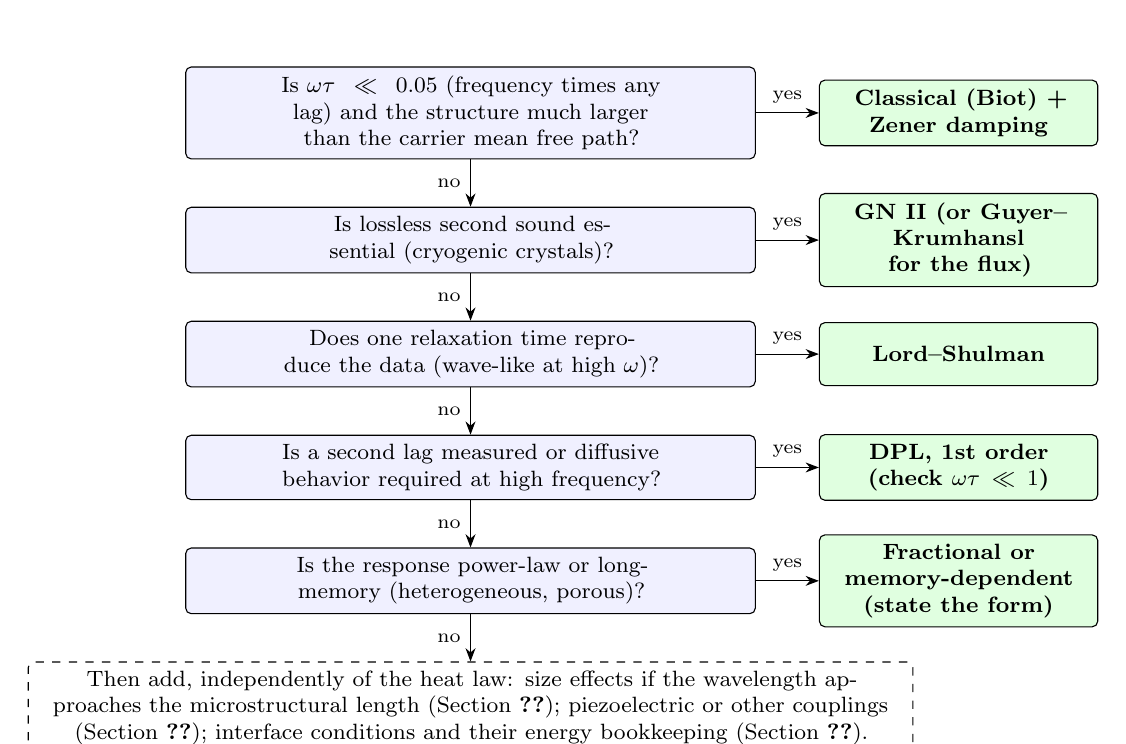
\begin{tikzpicture}[
 node distance=6mm and 8mm,
 q/.style={draw,rounded corners=2pt,fill=blue!6,align=center,font=\footnotesize,text width=7.0cm,minimum height=8mm},
 a/.style={draw,rounded corners=2pt,fill=green!12,align=center,font=\footnotesize\bfseries,text width=3.3cm,minimum height=8mm},
 >=Stealth]
\node[q] (q1) {Is $\omega\tau\ll0.05$ (frequency times any lag) and the structure much larger than the carrier mean free path?};
\node[a,right=of q1] (a1) {Classical (Biot) + Zener damping};
\node[q,below=of q1] (q2) {Is lossless second sound essential (cryogenic crystals)?};
\node[a,right=of q2] (a2) {GN II (or Guyer--Krumhansl for the flux)};
\node[q,below=of q2] (q3) {Does one relaxation time reproduce the data (wave-like at high $\omega$)?};
\node[a,right=of q3] (a3) {Lord--Shulman};
\node[q,below=of q3] (q4) {Is a second lag measured or diffusive behavior required at high frequency?};
\node[a,right=of q4] (a4) {DPL, 1st order (check $\omega\tau\ll1$)};
\node[q,below=of q4] (q5) {Is the response power-law or long-memory (heterogeneous, porous)?};
\node[a,right=of q5] (a5) {Fractional or memory-dependent (state the form)};
\draw[->] (q1)--(a1) node[midway,above,font=\scriptsize]{yes};
\draw[->] (q1)--(q2) node[midway,left,font=\scriptsize]{no};
\draw[->] (q2)--(a2) node[midway,above,font=\scriptsize]{yes};
\draw[->] (q2)--(q3) node[midway,left,font=\scriptsize]{no};
\draw[->] (q3)--(a3) node[midway,above,font=\scriptsize]{yes};
\draw[->] (q3)--(q4) node[midway,left,font=\scriptsize]{no};
\draw[->] (q4)--(a4) node[midway,above,font=\scriptsize]{yes};
\draw[->] (q4)--(q5) node[midway,left,font=\scriptsize]{no};
\draw[->] (q5)--(a5) node[midway,above,font=\scriptsize]{yes};
\node[draw,dashed,rounded corners=2pt,font=\footnotesize,below=of q5,text width=11cm,align=center] (add) {Then add, independently of the heat law: size effects if the wavelength approaches the microstructural length (Section~\ref{sec:size}); piezoelectric or other couplings (Section~\ref{sec:multi}); interface conditions and their energy bookkeeping (Section~\ref{sec:interfaces}).};
\draw[->] (q5)--(add) node[midway,left,font=\scriptsize]{no};
\end{tikzpicture}
\caption{Decision sequence for choosing a starting model. The threshold $\omega\tau\ll0.05$ follows from the regime map of \Cref{fig:regime}.}\label{fig:guide}
\end{figure}
\begin{summarybox}[Summary]
Comparative synthesis: for linear homogeneous media the template models with rational heat laws share one dispersion polynomial. Exact delays, fractional powers and hereditary kernels give transcendental or multivalued relations. Differences show in damping before speed, and only when $\omega\tau\gtrsim0.05$. LS and MGT have finite thermal fronts; classical, DPL, TPL and GN-III do not (first-order template). GN-II is unique in being energy-conserving. Piezoelectric stiffening is exact in the charge-free regime. Nonlocal lengths are calibration-dependent. At interfaces in lossy media, net flux is conserved but mode fractions need not sum to one.
\end{summarybox}


\section{A taxonomy of the field, and when two studies are comparable}\label{sec:taxonomy}

The literature labels a study ``generalized thermoelastic'' or it does not. The single label collapses several independent commitments into one word. A study may adopt a relaxation law for the heat flux, a gradient or
integral law for the stress, a coupling to a second field, and a validation regime. Each of these can
be varied while the others are held fixed. Two studies that share the label can therefore differ in the
mathematics of their governing equations, in their modal content and in the evidence they offer.
\Cref{sec:synthesis} compares families; this section says what a family \emph{is} as a coordinate, so that a
new model can be placed without argument.

The heat-flux template of \cref{sec:foundations} is a special case of Axis~2. Its flux law is local in
space and first order in the flux, with an optional thermal-displacement ($1/s$) term, and the lags are the coordinate that separates the template's members. A
model that needs an integral, fractional or gradient operator has left that axis rather than moved along
it. Such models therefore cannot be ranked against the template's members by setting a lag to zero.

The three groups of \cref{tab:taxonomy} (structure of the heat law, elastic constitutive law, additional fields) are a coarse, model-oriented view. In the five-axis scheme below, these commitments correspond mainly to the mathematical axis (Axis~2), both for the heat law and for the local, nonlocal or gradient form of the elastic law. The additional fields correspond to the physical and coupling axes (Axes~1 and 4). The wave and validation axes (Axes~3 and 5) describe what a study does with the model.

A study is classified by its vector of commitments $\mathbf{c}=(c_1,\dots,c_5)$, one coordinate per axis:

\begin{enumerate}[label=\textbf{Axis \arabic*:}]
\item \textbf{Physical axis (material class).} Classical elastic, thermoelastic, piezoelectric,
  piezothermoelastic, magneto-thermo-elastic, poroelastic, micropolar, two-temperature, semiconductor-like.
  The physical axis fixes which conserved quantities and driving fields exist, before any approximation is made.
\item \textbf{Mathematical axis (operator structure).} Local PDE, integro-differential, fractional-order,
  nonlocal gradient, hereditary memory integral, or variational/weak form. The most consequential
  differences between studies run along this axis.
\item \textbf{Wave axis (modal content).} Does the thermal mode propagate at finite speed; how many coupled
  modes exist; is there attenuation; what is the dispersion character of each.
\item \textbf{Coupling axis (field topology).} Which fields are coupled and how strongly:
  thermoelastic, thermo-piezoelectric, thermo-magneto-elastic, thermo-poro-elastic, thermo-micro-elastic.
  Coupling topology, and not the choice of energy functional, decides whether an interface problem is
  tractable.
\item \textbf{Validation axis (evidence regime).} Existence and uniqueness only; closed-form solution for a
  special geometry; numerical solution validated against a reference; comparison with experiment; a shared
  benchmark suite.
\end{enumerate}

Two studies are \emph{structurally} comparable, at the level of model class, when their vectors agree in the first two coordinates. A comparison of numbers further needs compatible geometry, parameters, boundary and interface conditions, nondimensional regime and observable. If they
differ there, a comparison of numbers means nothing and only a comparison of structure is available. To
make the weaker statement quantitative, define the axis-weight dissimilarity
\begin{equation}\label{eq:taxdissim}
d(\mathbf{c},\mathbf{c}')=\sum_{j=1}^{5} w_j\,\bigl(1-\delta_{c_j c_j'}\bigr),
\qquad
w_{\mathrm{math}}\ge w_{\mathrm{phys}}>w_{\mathrm{coup}}>w_{\mathrm{wave}}>w_{\mathrm{val}} ,
\end{equation}
with the ordering stated because it is a modeling decision open to challenge. A difference in the mathematical axis changes the governing operator and invalidates most direct comparisons. A difference in the validation axis changes only the epistemic status of the conclusion. The weights are reported whenever the dissimilarity is used, and no result in this review depends on their numerical values.

\begin{table}[H]\centering\small
\caption{The five axes with their admissible values. A study occupies one cell of the product; the last
column gives an example assignment for a coupled fractional piezothermoelastic problem.}
\label{tab:taxonomy-axes}
\begin{tabularx}{\textwidth}{@{}p{2.1cm}Y Y@{}}
\toprule
\textbf{Axis} & \textbf{Admissible values} & \textbf{Example} \\
\midrule
Physical & elastic; thermoelastic; piezoelectric; piezothermoelastic; magneto-thermo-elastic; poroelastic;
  micropolar; two-temperature; semiconductor & piezothermoelastic \\
Mathematical & local PDE; integro-differential; fractional; nonlocal gradient; hereditary; variational &
  fractional + local coupling \\
Wave & finite/infinite thermal speed; number of coupled modes; attenuating/non-attenuating &
  two modes, one attenuated \\
Coupling & none; thermal; thermal + electric; thermal + magnetic; thermal + poro; thermal + micro-rotation &
  thermal + electric \\
Validation & proof only; closed form; verified numerics; experiment; shared benchmark &
  verified numerics \\
\bottomrule
\end{tabularx}
\end{table}

A taxonomy earns its place only if it changes a decision, and this one changes three decisions in this review.
The taxonomy fixes the order in which \cref{sec:synthesis} compares families. It is also why \cref{sec:interfaces} insists that an energy flux be defined consistently with the model before ratios are compared (see \cref{sec:eqregister}). It is also why \cref{sec:open} keeps apart the questions that differ in the
mathematical axis from those that differ only in evidence.

\demoteclose

\section{Summary and Research Gaps}\label{sec:part_concl}
\demoteopen
\section{Open problems and research agenda}\label{sec:open}
\subsection{Theory}
\begin{enumerate}
\item \textbf{A classification theorem for the template.} For the first-order template no unstable root has been found numerically for DPL in a finite sweep of positive lags (an analytical statement is lacking), and the condition under which the thermal front has finite speed (the behavior of $sG(s)$ at large $s$) has been identified. What applied authors still lack is a complete analytical statement of well-posedness, decay and front structure for the coupled TPL and MGT systems with all parameters positive, that is, the conditions on $(\tau_q,\tau_T,\tau_v,k,k^*)$ together with the role of the coupling $\varepsilon$, in a form they can use directly.
\item \textbf{Thermodynamics of truncated lag models.} The time-differential DPL and TPL models raise questions of thermodynamic compatibility and continuous dependence \citep{Chirita2016,Tibullo2017}. A systematic account of which truncations admit an energy functional and an entropy inequality, and of what restrictions these impose on the lags, would resolve the confusion over the $\tau_T\ge\tau_q/2$ condition (Section~\ref{sec:lags}).
\item \textbf{Memory-dependent and fractional models.} Energy functionals, thermodynamic admissibility, uniqueness and finite-speed properties are not available for the memory-dependent and fractional laws at the generality of the template models. The high-frequency limit of the MDD law depends on the kernel (Section~\ref{sec:memory}), which suggests that a classification of kernels by $s\kappa(s)$ at large $s$ would be worth having.
\item \textbf{Interface conditions for lagged and memory models.} What is missing is a set of thermodynamically consistent interface conditions with thermal resistance for lagged and memory heat laws, including the entropy production at the interface (Section~\ref{sec:interfaces}).
\item \textbf{Mode interference in dissipative media.} Energy ratios will keep their ambiguity until there is a systematic way to apportion the energy flux among generated waves in lossy media.
\end{enumerate}
\subsection{Combined effects}
\begin{enumerate}
\setcounter{enumi}{5}
\item \textbf{Joint size and memory effects.} Authors compute combinations of nonlocal or gradient elasticity with hyperbolic or memory heat laws far more often than they validate them against lattice dynamics or atomistic simulation. A benchmark in which a lattice model with heat carriers supplies the reference dispersion would show which combination is justified.
\item \textbf{Calibration of length scales.} The calibration target, zone boundary or long wavelength, changes $\xi$ by about one third (Section~\ref{sec:size}); systematic calibration protocols for thermoelastic problems do not exist.
\item \textbf{Nonlocal forms of thermoelastic coupling.} The smoothed and unsmoothed forms of the thermal stress differ near the cut-off. The thermodynamically consistent form should be derived from a nonlocal free energy rather than chosen.
\item \textbf{Surface and interface thermoelasticity at the nanoscale.} Surface stress, surface heat capacity and Kapitza resistance modify both surface waves and interface partition in ways that the bulk models treated here do not capture.
\end{enumerate}
\subsection{Experiments and data}
\begin{enumerate}
\setcounter{enumi}{9}
\item \textbf{Measurement of both branches.} Most of the present evidence is indirect. An experiment that measured the elastic-type and the thermal-type branch in the same solid across the crossover frequency would discriminate among heat laws.
\item \textbf{Independent determination of lags.} Relaxation times and lags are generally obtained by fitting. An independent measurement, from pump--probe experiments together with ultrasonic damping for instance, would test the models instead of fitting them.
\item \textbf{Thermoelastic damping at ultra-high frequency.} Resonators at gigahertz frequencies already reach the regime in which lagged corrections matter; systematic data on damping against frequency and size would calibrate them.
\end{enumerate}
\subsection{Computation}
\begin{enumerate}
\setcounter{enumi}{12}
\item \textbf{Benchmark suite.} A set of agreed benchmark problems, namely the heat pulse, thermal shock, Rayleigh wave and interface problems of this review, with reference solutions at specified precision, would improve the reliability of numerical codes.
\item \textbf{Efficient memory operators.} Fast algorithms for fractional and memory-dependent operators in time-domain codes, with error control.
\end{enumerate}

\begin{summarybox}[Summary]
Open problems: (theory) classification theorem for the template, thermodynamics of truncated lag models, memory-model energy functionals, consistent interface conditions for lagged/memory laws, mode-interference framework for dissipative media. (combined effects) joint size-and-memory validation against lattice dynamics, calibration protocols for length scales, thermodynamically consistent nonlocal thermal stress, nanoscale surface/interface thermoelasticity. (experiments) measure both branches in the same solid, independent lag determination, ultra-high-frequency damping data. (computation) agreed benchmark suite, fast memory operators.
\end{summarybox}

\subsection{Researchable questions, and what would settle each}\label{sec:research_questions}

The agenda above states the gaps. A gap becomes usable only when the evidence that would close it is
stated as well, since that is what lets a reader judge whether a proposed study is decisive or merely
related. The table makes the test explicit, and its final column names the section where the gap is first
stated in this paper. \Cref{tab:research-questions} lists, for each gap, what would settle it.

\begin{table}[H]\centering\small
\caption{Researchable questions. Each row restates a gap stated in \cref{sec:open}; the third column
names the evidence that would move it from open to closed. No new claim is introduced.}
\label{tab:research-questions}
\begin{tabularx}{\textwidth}{@{}p{0.5cm}Y Y p{1.75cm}@{}}
\toprule
\textbf{\#} & \textbf{Question} & \textbf{What would settle it} & \textbf{Stated in} \\
\midrule
R1 & What is the total (not availability) energy flux for each generalized family, and how does it
  differ from the flux used for interface partition? & A time-domain derivation per family under an
  explicit free-energy convention, external-field power terms and boundary conditions, checked against
  the primary formulation, together with a statement of the first-order reduction that recovers the flux
  used for the energy ratios. & \cref{sec:foundations}, \cref{sec:interfaces} \\
R2 & Is energy conserved at an interface in generalized and nonlocal media, and in what sense? & An
  interface balance derived from the selected model's flux, with the admissible jump conditions, checked
  against a benchmark whose reference solution does not depend on the model under test. &
  \cref{sec:interfaces} \\
R3 & Which benchmark is the right reference for a generalized theory? & A specification whose reference
  solution is independent (analytic limit, symbolic determinant, or an independently implemented
  discretization), with a stated tolerance. & \cref{app:registry} \\
R4 & Do the predicted generalized modes exist in a real material, with the predicted attenuation? & An
  experimental measurement of the predicted observables under conditions inside the model's stated
  validity domain. & \cref{sec:experiments} \\
R5 & How should energy flux and energy partition be normalized across families so that comparisons mean
  something? & A normalization in terms of physical observables rather than model parameters. &
  \cref{sec:synthesis} \\
R6 & How are nonlocal interface conditions and a nonlocal divergence theorem formulated? & A variational
  statement of the nonlocal boundary-value problem from which the interface conditions follow rather than
  are assumed. & \cref{sec:size} \\
R7 & Are phase-lag, memory-kernel and anisotropy parameters identifiable from measurable data? & The
  number and type of independent measurements needed to separate the parameters, established by analysis
  of the sensitivity structure or by a designed experiment; the answer is model-specific. &
  \cref{sec:experiments} \\
R8 & Do the thermodynamic restrictions reduce the admissible parameter set under anisotropic symmetry as
  they do in the isotropic case? & The anisotropic admissibility analysis carried through for each family,
  with the coordinate-free form of the fractional and memory operators under anisotropic differentiation.
  & \cref{sec:foundations} \\
R9 & Which comparative statements survive when each family's own conventions are respected? & A
  model-by-model full-text check of constitutive conventions, free energies and external-field power terms
  before any flux or mode count is compared. & \cref{sec:synthesis} \\
R10 & Can the benchmarks be reproduced from published inputs, and at what convergence rate? & Shared
  implementations, published inputs and reported convergence rates for every benchmark. &
  \cref{sec:methods} \\
\bottomrule
\end{tabularx}
\end{table}

R1 and R9 are the same question at different depths. A family-level flux comparison cannot be trusted
until the model-specific derivations behind it exist, which is why the register in \cref{sec:eqregister}
marks the affected entries open instead of filling them.

\section{Conclusions}\label{sec:conclusions}
Generalized thermoelasticity is a family organized by the function $G(s)$ that relates heat flux to temperature gradient, together with choices of elastic law and added fields, and not a collection of unrelated theories. That organization buys three kinds of result. It gives exact statements about reductions and limits, among them the clarification that the often-quoted DPL stability condition belongs to a specific truncation and that GN-III has no finite front speed. It gives a dispersion polynomial for linear homogeneous media and rational heat laws, from which comparative speeds, attenuation and thermoelastic damping follow, and which shows that the heat law affects damping long before it affects speed, and only for $\omega\tau\gtrsim0.05$. It gives problem-level results: finite fronts and surface jumps in heat pulses, the structure of thermoelastic Rayleigh waves, the renormalization by piezoelectric coupling, the calibration dependence of nonlocal lengths, and the distinction between net energy flux and mode-by-mode fractions at interfaces in lossy media. Many of the open questions concern validation rather than derivation: independent measurement of lags, joint validation of size and memory effects against lattice dynamics, and benchmark solutions. The unified notation, the verified reductions, the pitfalls checklist and the decision guide are there so that readers can choose, justify and check models, and the open problems so that effort goes where it is most needed.

\demoteclose


\newpage

%================== BACK MATTER ==================
\section*{Acknowledgements}\addcontentsline{toc}{section}{Acknowledgements}
The author thanks colleagues at Gurugram University for discussions on generalized thermoelasticity. The numerical computations accompanying this manuscript were used to verify all reported dispersion relations, damping curves and energy-partition results.

\section*{Declarations}\label{sec:declarations}
\addcontentsline{toc}{section}{Declarations}

\subsection*{Author contributions (CRediT)}
\textbf{Vipin Gupta:} Conceptualization; Methodology; Software; Validation; Formal analysis;
Investigation; Data curation; Writing -- original draft; Writing -- review and editing;
Visualization; Supervision; Project administration.

\subsection*{Funding}
This research received no funding.

\subsection*{Competing interests}
The author declares no conflict of interest.

\subsection*{Data and code availability}
The computations that produce every computed figure and every benchmark in \cref{app:repro} and
\cref{app:registry} come with the manuscript, together with the parameter registers in
\cref{app:params}. No experimental data were generated in this work; every experimental value quoted is
attributed to its source in the text.

\subsection*{Use of generative tools}
Generative AI tools were used in preparing this manuscript: for drafting and language editing, for writing and running the verification computations, for checking notation and cross-references, and for literature and claim checks whose results are summarized in the evidence protocol (\cref{sec:evidence_protocol}). The author reviewed the content and is responsible for it; the tools are not authors. Not every cited work was read page by page, and the claim register records which attributions were checked against the printed source and which were not.


\section*{Nomenclature}\addcontentsline{toc}{section}{Nomenclature}\label{app:nomenclature}
Indices follow the Einstein summation convention; a comma denotes a spatial derivative and a dot a time derivative. The strain tensor is written with two indices ($\varepsilon_{ij}$) so that it is not confused with the scalar coupling $\varepsilon$. The unstarred $k$ is the thermal conductivity in $G$ and in tables, and the wavenumber in $\exp[\ii(kx-\omega t)]$ and in dispersion relations, where $K=k^2$; the symbol $K^2$ is the electromechanical coupling and is used only in the piezoelectric sections. The unindexed $c$ is always the specific heat. Plane waves are $\exp[\ii(kx-\omega t)]$ with $\Imag k\ge0$ for spatial decay in the propagation direction, and a ``branch'' of the dispersion relation is a root $k(\omega)$ followed by continuity in $\omega$.

\medskip\noindent\textbf{Latin symbols}
\begin{tabbing}
\hspace{3.2cm}\=\kill
$G(s)$ \> heat-flux function\\
$K=k^2$ \> squared wavenumber in dispersion polynomials\\
$K^2$ \> electromechanical coupling\\
$T_0$ \> reference temperature\\
$Z=\rho c_1$ \> mechanical impedance\\
$c$ \> specific heat at constant strain\\
$c_1=\sqrt{(\lambda+2\mu)/\rho}$ \> isothermal P-wave speed\\
$c_2=\sqrt{\mu/\rho}$ \> shear wave speed\\
$c_T$ \> thermal wave speed\\
$k,\ k^*$ \> conductivities (Fourier, Green--Naghdi)\\
$q_i$ \> heat flux\\
$s=-\ii\omega$ \> Laplace variable (complex frequency)\\
$u_i$ \> displacement\\
$v$ \> thermal displacement, $\dot v=\theta$\\
\end{tabbing}

\medskip\noindent\textbf{Greek symbols}
\begin{tabbing}
\hspace{3.2cm}\=\kill
$\alpha=k/\rho c$ \> thermal diffusivity (written $\chi$ in the kinetic, nanoscale and thermal-mode sections)\\
$\alpha_T$ \> linear expansion coefficient\\
$\beta=(3\lambda+2\mu)\alpha_T$ \> thermal-stress coefficient\\
$\varepsilon=\beta^2T_0/(\rho^2cc_1^2)$ \> thermoelastic coupling\\
$\varepsilon_{ij}$ \> strain\\
$\theta=T-T_0$ \> temperature increment\\
$\lambda,\ \mu$ \> Lam\'e constants\\
$\xi,\ \ell$ \> nonlocal and gradient lengths\\
$\rho$ \> mass density\\
$\sigma_{ij}$ \> stress\\
$\tau_q,\ \tau_T,\ \tau_v$ \> relaxation time and lags\\
$\tau_R,\ \tau_N$ \> resistive and normal phonon relaxation times\\
$\omega$ \> angular frequency\\
$\omega_*=\rho cc_1^2/k$ \> thermal characteristic frequency\\
\end{tabbing}

\medskip\noindent\textbf{Subscripts and superscripts}
\begin{tabbing}
\hspace{3.2cm}\=\kill
$0$ \> reference state\\
$i,\ j,\ k$ \> tensor indices\\
$(\,)_{,i}$ \> spatial derivative\\
$\dot{(\,)}$ \> time derivative\\
$(\,)^*$ \> Green--Naghdi quantity\\
\end{tabbing}


%================== APPENDICES ==================
\appendix
\section{Derivations of the balance laws}\label{app:balance}

This appendix records where each balance used in \cref{sec:foundations} comes from and what it assumes, so that a reader can see which statements are identities of continuum mechanics and which already contain a constitutive choice. Every derivation below is algebra on the stated assumptions, and none of them uses a heat law.

\subsection*{Linear momentum}
Take an arbitrary material volume $V$ with surface $\partial V$ and outward normal $n_i$. Cauchy's
postulate gives the surface traction $t_i=\sigma_{ji}n_j$. Requiring that the rate of change of linear momentum
equal the resultant force for \emph{every} $V$,
$\frac{\dd}{\dd t}\int_V\rho\dot u_i\,\dd V=\int_{\partial V}\sigma_{ji}n_j\,\dd S+\int_V\rho f_i\,\dd V$,
and applying the divergence theorem together with the transport theorem gives
$\rho\ddot u_i=\sigma_{ji,j}+\rho f_i$ after the volume is shrunk to a point. The assumptions are that a Cauchy
stress exists (no couple stresses), that the motion is described by a single displacement field, and that the body is
non-polar. These are exactly the assumptions recorded for \eqref{eq:mom}.

\subsection*{Symmetry of the stress}
The same argument applied to the moment of momentum about a point, with no body couples and no couple
stresses, leaves $\int_V e_{ijk}\sigma_{jk}\,\dd V=0$ for every $V$, hence $\sigma_{ij}=\sigma_{ji}$. The
conclusion follows from the assumptions and is not an independent law: in a micropolar or couple-stress
continuum the stress is not symmetric, and the derivation must be redone with the couple-stress tensor.

\subsection*{Mechanical power}
Contracting the momentum balance \eqref{eq:mom} with the velocity and using the symmetry of the stress gives
\begin{equation}
\rho\frac{\dd}{\dd t}\Bigl(\tfrac12\dot u_i\dot u_i\Bigr)=\bigl(\sigma_{ij}\dot u_i\bigr)_{,j}
-\sigma_{ij}\dot\varepsilon_{ij}+\rho f_i\dot u_i ,
\end{equation}
so the stress power $\sigma_{ij}\dot\varepsilon_{ij}$ is the only term that exchanges mechanical energy with
the internal state. Here the strain enters, and not the displacement gradient: the rotation does no work.

\subsection*{Internal energy}
If the internal energy of a material volume changes by the heat supplied plus the stress power
delivered, then with heat flux $q_i$ and supply $r$,
\begin{equation}
\rho\dot e=\sigma_{ij}\dot\varepsilon_{ij}-q_{i,i}+\rho r ,
\end{equation}
which is the second line of \eqref{eq:mom}. This is an axiom of the theory: it defines what $e$ means, and
a generalized theory that changes the flux $q_i$ or adds a state variable must restate it.

\subsection*{The exact Eulerian flux}
Adding the power balance and the internal-energy balance gives the material-derivative form
$\rho\frac{\dd}{\dd t}\bigl(\tfrac12\dot u_i\dot u_i+e\bigr)+\bigl(q_j-\sigma_{ji}\dot u_i\bigr)_{,j}
=\rho f_i\dot u_i+\rho r$. Converting the material derivative with mass conservation yields
\eqref{eq:exactflux}. The last step is the one the literature often skips: the material form is not the
fixed-volume form, and the difference is the advection term $\mathcal E_{\mathrm{tot}}\dot u_j$.
Omitting it is legitimate only as a first-order reduction under the small-motion assumptions stated with
\eqref{eq:exactflux-balance}.
\label{app:balance_ref}
\section{Derivation and verification of the dispersion polynomial}\label{app:disp}
With $\partial_x\to\ii k$ and $\partial_t\to s=-\ii\omega$, the momentum and energy balances \eqref{eq:1d} for the template give the linear system
\begin{align}
\bigl(\rho s^2+\rho c_1^2k^2\bigr)\hat u+\ii\beta k\,\hat\theta&=0,\\
T_0\beta\,s\,\ii k\,\hat u+\bigl(s\rho c+G(s)k^2\bigr)\hat\theta&=0,
\end{align}
where the second equation uses $\ii k\,\hat q=-\ii k\,G\,\ii k\,\hat\theta=Gk^2\hat\theta$. Its determinant is
$(\rho c_1^2k^2+\rho s^2)(s\rho c+Gk^2)+\beta^2T_0\,s\,k^2$ (since $(\ii k)(\ii k)=-k^2$), which is \eqref{eq:disp} because $\rho s^2=-\rho\omega^2$. The identity was checked symbolically with every template parameter kept as a symbol (dispersion check). A first version of the implementation used here had the coupling term with the opposite sign, and the symbolic comparison caught it at once. That is why the check is recommended.

\paragraph{Unified form for LS and GL.} Multiplying by $1+\tau_0s$ for $G=k/(1+\tau_0s)$ gives \eqref{eq:unified} with $\tau^\dagger=\tau_0$; the Green--Lindsay system of \eqref{eq:GL} gives the same polynomial with $\tau^\dagger=\tau_1$, since the thermal-stress term carries $(1+\tau_1s)$.

\paragraph{Limits.} Setting $\beta\to0$ decouples the roots into $K=-s^2/c_1^2$ and $K=-s\rho c/G$; the latter reduces for $G=k$ to $k^2=\ii\omega/\alpha$, with phase speed $\sqrt{2\alpha\omega}$.

\paragraph{Nonlocal forms.} If the stress law is $(1-\xi^2\partial_x^2)\sigma=\rho c_1^2\,u_{,x}-\beta\theta$ (form A of Section~\ref{sec:size}), the momentum balance becomes $[\rho s^2(1+\xi^2K)+\rho c_1^2K]\hat u+\ii\beta k\hat\theta=0$ and the determinant is $[\rho s^2(1+\xi^2K)+\rho c_1^2K](s\rho c+GK)+\beta^2T_0sK=0$; for form B the last term is multiplied by $1+\xi^2K$.
\label{app:disp_ref}
\section{Characteristic numbers and parameter estimates}\label{app:numbers}
The dimensionless groups that control a thermoelastic wave problem are collected in \Cref{tab:groups} for a given solid and heat-flux model.
\begin{table}[ht]\centering\small
\caption{Dimensionless groups for thermoelastic wave problems.}\label{tab:groups}
\begin{tabular}{@{}llp{6.2cm}@{}}\toprule
Group & Definition & Meaning\\\midrule
$\varepsilon$ & $\beta^2T_0/(\rho^2cc_1^2)$ & adiabatic--isothermal modulus difference\\
$\omega_*$ & $\rho cc_1^2/k$ & frequency at which conduction over a wavelength matches the period\\
$\omega\tau$ & $\omega\tau_q$ & frequency times flux lag\\
$c_T/c_1$ & $\sqrt{k/(\rho c\tau_0)}/c_1=1/\sqrt{\tau_0\omega_*}$ & thermal-to-elastic front speed\\
$\tau_T/\tau_q$ & & lag ratio (DPL)\\
$\xi\omega_*/c_1$ & & nonlocal length in thermal units\\
$K^2$ & $e^2/(\varepsilon_ec)$ & electromechanical coupling\\
\bottomrule\end{tabular}
\end{table}
Since $c_T/c_1=1/\sqrt{\tau_0\omega_*}$, the thermal front outruns the elastic one for $\tau_0\omega_*<1$ and falls behind it for $\tau_0\omega_*>1$, and the two branches hybridize near $\tau_0\omega_*\approx1$ (\Cref{fig:regime}). With the values of \cref{tab:materials} and a lag time of one picosecond, $\tau_0\omega_*\approx0.4$ for aluminum, so the thermal front is somewhat the faster.
\label{app:numbers_ref}
\section{Reproducibility: computations and what each one verifies}\label{app:repro}
Every numerical result in this review comes from computations supplied with the manuscript. \Cref{tab:scripts} lists them with the checks each performs.
\begin{table}[H]\centering\footnotesize
\caption{Computations and the identities or limits they verify.}\label{tab:scripts}
\begin{tabularx}{\textwidth}{@{}p{5.2cm}X@{}}\toprule
Check or figure & Content and checks\\\midrule
dispersion check & Symbolic determinant of the field equations equals the dispersion polynomial \eqref{eq:disp} (difference zero).\\
reduction check & Reductions of $G(s)$: DPL$\to$LS, TPL$\to$DPL, GN-II/III, large-$s$ limits.\\
front-speed check & LS and GL front speeds from the polynomial agree with \eqref{eq:fronts} to four digits.\\
GN-II check & GN-II speeds are non-dispersive and equal the formula.\\
thermopiezoelectric check & Thermopiezoelectric determinant is proportional to the renormalized thermoelastic polynomial \eqref{eq:renorm}.\\
dispersion figure, Zener-damping figure & Dispersion and damping; weak-coupling Debye result confirmed ($Q^{-1}/\varepsilon=0.4999998$).\\
stability figure & Growth rates for the 1st- and 2nd-order DPL truncations.\\
heat-pulse figure & Cattaneo pulse by Talbot inversion; Fourier limit and front exactness.\\
thermal-shock figure & Thermal shock of a coupled half-space; boundary conditions satisfied to machine precision.\\
Rayleigh-wave figure & Thermoelastic Rayleigh root; $\varepsilon\to0$ limit gives the elastic Rayleigh speed.\\
interface calculation, interface-energy figure & Elastic and thermoelastic interface; impedance limit to twelve digits; net-flux continuity to $10^{-15}$.\\
lattice figure, nonlocal thermoelastic figure & Lattice calibration of $\xi$; nonlocal thermoelastic branches; $\xi\to0$ and $\varepsilon\to0$ limits.\\
fractional and MDD figure & Caputo heat equation (erfc check) and MDD kernel transform ($\kappa(0)=1/3$).\\
regime-map figure, Laplace-inversion benchmark, materials table & Regime map; Laplace-inversion benchmark; material coupling table.\\
lag-truncation figure & Exact delay law versus first- and second-order truncations; relative errors; sign change of attenuation at $\omega\tau=\pi/2$.\\
flexural-damping figure, Lamb-wave calculation, Lamb-wave figure & Zener versus Lifshitz--Roukes; plate determinant matches exact Rayleigh--Lamb to $10^{-10}$ in the elastic limit and the Lifshitz--Roukes loss (plane-strain $\Delta$) with ratio $1.000$ at small $kh$.\\
coupled-fractional figure, bar-mode figure, Guyer--Krumhansl figure & Coupled fractional dispersion; clamped-bar modal loss; Guyer--Krumhansl thermal branch (high-frequency limit confirmed to $0.2\%$).\\
anisotropy figure, reflection figure, Bleustein--Gulyaev check & Cubic-crystal coupling by direction; free-surface reflection (elastic limit to $10^{-10}$); Bleustein--Gulyaev closed forms versus secular determinant.\\
finite-difference benchmark, Kramers--Kronig check & Finite-difference orders for the Cattaneo front; Kramers--Kronig sum rule to a few parts in $10^{6}$.\\
worked-example calculation, scenario table, catalog generator, reference-list assembly & Numbers of the worked examples; application-regime table; classified catalog of the references; assembly of the supplementary bibliographic file (Crossref records and author-library entries, de-duplicated by DOI and title).\\
\bottomrule\end{tabularx}
\end{table}
\paragraph{Running the checks.} Fourteen of the computations (the dispersion, admissibility, layered-media, identifiability, modulus, Lamb-wave, reduction, thermopiezoelectric, front-speed, GN-II, Kramers--Kronig and Bleustein--Gulyaev checks, and the Laplace-inversion and finite-difference benchmarks) are accompanied by explicit acceptance criteria with stated tolerances, and a computation that misses its tolerance is reported as a failure. All fourteen are run together and their outcomes are logged. A pass verifies the stated identity or limit to the stated tolerance, and a $10^{-10}$ match of an elastic limit verifies that limit only; it does not verify the physical validity of a model. The numerical output of every figure and check computation is archived, so a number quoted in the text can be traced to a printed value; quantities read off a figure, such as peak positions and percentage levels, are approximate and are not archived. Library versions used are recorded with the computations.
\paragraph{Limits of verification.} The computations verify the mathematics of the models stated here against their own field equations and limiting cases. They do not verify that a model describes a given material, which requires comparison with experiment. The material values in \cref{tab:materials} are rounded handbook-type numbers used for illustration.
\label{app:repro_ref}
\section{Classified catalog of the cited literature}\label{app:catalogue}
A classified selection of the cited works (323 of the 425) is listed, grouped by the subject of its title, and works not discussed in the main text are included as further reading for the corresponding topic. The grouping is automatic, by title keyword alone, so it helps to locate the literature without summarizing any paper. Entries are ordered by the year in the citation key within a group, and a work whose title touches several topics appears once, under the first matching group.
\subsection{Second sound, phonon transport and kinetic theory}
\begin{itemize}\itemsep0pt\small
\item \citet{Chester1963}: \emph{Second Sound in Solids}; Physical Review.
\item \citet{Ackerman1966}: \emph{Second sound in solid helium}; Physical Review Letters.
\item \citet{GuyerKrumhansl1966}: \emph{Solution of the linearized phonon Boltzmann equation}; Physical Review.
\item \citet{GuyerKrumhansl1966II}: \emph{Thermal Conductivity, Second Sound, and Phonon Hydrodynamic Phenomena in Nonmetallic Crystals}; Physical Review.
\item \citet{Jackson1970}: \emph{Second sound in NaF}; Physical Review Letters.
\item \citet{McNelly1970}: \emph{Heat pulses in NaF: onset of second sound}; Physical Review Letters.
\item \citet{Chandrasekharaiah1986}: \emph{Thermoelasticity with second sound: a review}; Applied Mechanics Reviews.
\item \citet{Thomsen1986}: \emph{Surface generation and detection of phonons by picosecond light pulses}; Physical Review B.
\item \citet{Huberman2019}: \emph{Observation of second sound in graphite at temperatures above 100 K}; Science.
\end{itemize}
\subsection{Dual-phase-lag, three-phase-lag and delay models}
\begin{itemize}\itemsep0pt\small
\item \citet{Tzou1997}: \emph{Macro-to-microscale heat transfer: the lagging behavior}; CRC Press.
\item \citet{Antaki2000}: \emph{Effect of dual-phase-lag heat conduction on ignition of a solid}; Journal of Thermophysics and Heat Transfer.
\item \citet{Quintanilla2002b}: \emph{Exponential stability in the dual-phase-lag heat conduction theory}; Journal of Non-Equilibrium Thermodynamics.
\item \citet{Quintanilla2003DPL}: \emph{A Condition on the Delay Parameters in the One-Dimensional Dual-Phase-Lag Thermoelastic Theory}; Journal of Thermal Stresses.
\item \citet{Quintanilla2006}: \emph{A note on stability in dual-phase-lag heat conduction}; International Journal of Heat and Mass Transfer.
\item \citet{RoyChoudhuri2007}: \emph{On A Thermoelastic Three-Phase-Lag Model}; Journal of Thermal Stresses.
\item \citet{Quintanilla2008}: \emph{End effects in three-phase-lag heat conduction}; Applicable Analysis.
\item \citet{Quintanilla2008a}: \emph{A note on stability in three-phase-lag heat conduction}; International Journal of Heat and Mass Transfer.
\item \citet{Quintanilla2009}: \emph{A well-posed problem for the three-dual-phase-lag heat conduction}; Journal of Thermal Stresses.
\item \citet{Miranville2010}: \emph{A phase-field model based on a three-phase-lag heat conduction}; Applied Mathematics \& Optimization.
\item \citet{Abouelregal2011}: \emph{Rayleigh waves in a thermoelastic solid half space using dual-phase-lag model}; International Journal of Engineering Science.
\item \citet{Fabrizio2014}: \emph{Stability and second law of thermodynamics in dual-phase-lag heat conduction}; International Journal of Heat and Mass Transfer.
\item \citet{Rukolaine2014}: \emph{Unphysical effects of the dual-phase-lag model of heat conduction}; International Journal of Heat and Mass Transfer.
\item \citet{Xu2015}: \emph{Time fractional dual-phase-lag heat conduction equation}; Chinese Physics B.
\item \citet{Chirita2016}: \emph{The time differential three-phase-lag heat conduction model: Thermodynamic compatibility and continuous dependence}; International Journal of Heat and Mass Transfer.
\item \citet{Ezzat2016b}: \emph{On dual-phase-lag thermoelasticity theory with memory-dependent derivative}; Mechanics of Advanced Materials and Structures.
\item \citet{Chirita2017}: \emph{High-order approximations of three-phase-lag heat conduction model: some qualitative results}; Journal of Thermal Stresses.
\item \citet{Julius2017}: \emph{Nonhomogeneous dual-phase-lag heat conduction problem: analytical solution and select case studies}; Journal of Heat Transfer.
\item \citet{Tibullo2017}: \emph{On the thermomechanical consistency of the time differential dual-phase-lag models of heat conduction}; International Journal of Heat and Mass Transfer.
\item \citet{Abouelregal2019}: \emph{Three-phase-lag thermoelastic heat conduction model with higher-order time-fractional derivatives}; Indian Journal of Physics.
\item \citet{Biswas2019}: \emph{Modeling of memory-dependent derivatives in orthotropic medium with three-phase-lag model under the effect of magnetic field}; Mechanics Based Design of Structures and Machines.
\item \citet{Gupta2019}: \emph{A study on generalized thermoelasticity theory based on non-local heat conduction model with dual-phase-lag}; Journal of Thermal Stresses.
\item \citet{Singh2019}: \emph{Thermoelastic interaction in the semi-infinite solid medium due to three-phase-lag effect involving memory-dependent derivative}; Journal of Thermal Stresses.
\item \citet{AboDahab2020}: \emph{Fractional derivative order analysis and temperature-dependent properties on p- and SV-waves reflection under initial stress and three-phase-lag model}; Results in Physics.
\item \citet{Abouelregal2020}: \emph{A generalized heat conduction model of higher-order time derivatives and three-phase-lags for non-simple thermoelastic materials}; Scientific Reports.
\item \citet{Abouelregal2020a}: \emph{Generalized mathematical novel model of thermoelastic diffusion with four phase lags and higher-order time derivative}; The European Physical Journal Plus.
\item \citet{Kumar2020}: \emph{Thermoelastic damping analysis for size-dependent microplate resonators utilizing the modified couple stress theory and the three-phase-lag heat conduction model}; International Journal of Heat and Mass Transfer.
\item \citet{Singh2020a}: \emph{Eigenfunction approach to generalized thermo-viscoelasticity with memory dependent derivative due to three-phase-lag heat transfer}; Journal of Thermal Stresses.
\item \citet{Xue2020}: \emph{Size-dependent thermoelasticity of a finite bi-layered nanoscale plate based on nonlocal dual-phase-lag heat conduction and Eringen's nonlocal elasticity}; Applied Mathematics and Mechanics.
\item \citet{Yang2020}: \emph{Nonlocal dual-phase-lag heat conduction and the associated nonlocal thermal-viscoelastic analysis}; International Journal of Heat and Mass Transfer.
\item \citet{Abouelregal2021}: \emph{Generalized thermoelasticity based on higher-order memory-dependent derivative with time delay}; Results in Physics.
\item \citet{Bayones2021}: \emph{Effect of moving heat source on a magneto-thermoelastic rod in the context of Eringen’s nonlocal theory under three-phase lag with a memory dependent derivative}; Mechanics Based Design of Structures and Machines.
\item \citet{Li2021}: \emph{Fractional order thermo-viscoelastic theory of biological tissue with dual phase lag heat conduction model}; Applied Mathematical Modeling.
\item \citet{Satish2021}: \emph{Thermoelastic damping in nonlocal rod using three-phase lag heat conduction model}; Journal of Thermal Stresses.
\item \citet{Tiwari2021}: \emph{Analysis of plane wave propagation under the purview of three phase lag theory of thermoelasticity with non-local effect}; European Journal of Mechanics - A/Solids.
\item \citet{Yang2021}: \emph{Dual-phase-lag thermoelastic damping in nonlocal rectangular nanoplates}; Waves in Random and Complex Media.
\item \citet{vanDerMerwe2021}: \emph{Comparing the dual phase lag, Cattaneo-Vernotte and Fourier heat conduction models using modal analysis}; Applied Mathematics and Computation.
\item \citet{Miranville2022}: \emph{Parabolic phase-lag heat conduction theories revisited}; Applied Mathematics Letters.
\item \citet{Tiwari2022}: \emph{Non-local effect on quality factor of micro-mechanical resonator under the purview of three-phase-lag thermoelasticity with memory-dependent derivative}; Applied Physics A.
\item \citet{Kumar2023}: \emph{Analysis of Waves at Boundary Surfaces at Distinct Media with Nonlocal Dual-Phase-Lag}; Proceedings of the National Academy of Sciences, India Section A: Physical Sciences.
\item \citet{Kumar2023PhysScr}: \emph{Energy ratio response at the interface of elastic and dual-porous thermoelastic half-spaces}; Physica Scripta.
\item \citet{Das2024}: \emph{Size-dependent effect on the interaction of surface waves in micropolar thermoelastic medium with dual pore connectivity}; Physica Scripta.
\item \citet{Pathania2024}: \emph{Three-phase-lag analysis of transversely isotropic double porous thermoelastic waves with liquid medium}; Physica Scripta.
\item \citet{Das2025}: \emph{Fractional and memory effects on wave reflection in pre-stressed microstructured solids with dual porosity}; European Journal of Mechanics - A/Solids.
\item \citet{Aldandani2026a}: \emph{On the Rayleigh surface wave dynamics of porous piezo-thermoelectric smart material with spatio-temporal nonlocality and fractional higher-order three-phase-lag theory}; Scientific Reports.
\end{itemize}
\subsection{Green--Naghdi, Green--Lindsay and extended thermodynamics}
\begin{itemize}\itemsep0pt\small
\item \citet{Biot1956}: \emph{Thermoelasticity and irreversible thermodynamics}; Journal of Applied Physics.
\item \citet{Coleman1963}: \emph{The thermodynamics of elastic materials with heat conduction and viscosity}; Archive for Rational Mechanics and Analysis.
\item \citet{Lord1967}: \emph{A generalized dynamical theory of thermoelasticity}; Journal of the Mechanics and Physics of Solids.
\item \citet{McCarthy1972}: \emph{Wave propagation in generalized thermoelasticity}; International Journal of Engineering Science.
\item \citet{Dhaliwal1980}: \emph{Generalized thermoelasticity for anisotropic media}; Quarterly of Applied Mathematics.
\item \citet{Bem1982}: \emph{Existence of a generalized solution in thermoelasticity with one relaxation time}; Journal of Thermal Stresses.
\item \citet{Bem1983}: \emph{Existence of a generalized solution in thermoelasticity with two relaxation times, part II}; Journal of Thermal Stresses.
\item \citet{Green1993}: \emph{Thermoelasticity without energy dissipation}; Journal of Elasticity.
\item \citet{Sherief1993}: \emph{State space formulation for generalized thermoelasticity with one relaxation time including heat sources}; Journal of Thermal Stresses.
\item \citet{Chandrasekharaiah1996}: \emph{A uniqueness theorem in the theory of thermoelasticity without energy dissipation}; Journal of Thermal Stresses.
\item \citet{Chandrasekharaiah1997}: \emph{Complete solutions in the theory of thermoelasticity without energy dissipation}; Mechanics Research Communications.
\item \citet{Iesan1998}: \emph{On the theory of thermoelasticity without energy dissipation}; Journal of Thermal Stresses.
\item \citet{MuellerRuggeri1998}: \emph{Rational Extended Thermodynamics}; Springer.
\item \citet{Suh1998}: \emph{Effects of Thermomechanical Coupling and Relaxation Times on Wave Spectrum in Dynamic Theory of Generalized Thermoelasticity}; Journal of Applied Mechanics.
\item \citet{Ciarletta1999}: \emph{A theory of micropolar thermoelasticity without energy dissipation}; Journal of Thermal Stresses.
\item \citet{HetnarskiIgnaczak1999}: \emph{Generalized thermoelasticity}; Journal of Thermal Stresses.
\item \citet{Quintanilla1999}: \emph{On the spatial behavior in thermoelasticity without energy dissipation}; Journal of Thermal Stresses.
\item \citet{Verma2001}: \emph{Wave propagation in plates of general anisotropic media in generalized thermoelasticity}; International Journal of Engineering Science.
\item \citet{Quintanilla2002}: \emph{Thermoelasticity without energy dissipation of materials with microstructure}; Applied Mathematical Modeling.
\item \citet{Quintanilla2002a}: \emph{Existence in thermoelasticity without energy dissipation}; Journal of Thermal Stresses.
\item \citet{Sinha2003}: \emph{Eigenvalue approach to study the effect of rotation and relaxation time in generalized thermoelasticity}; Computers \& Mathematics with Applications.
\item \citet{Ezzat2004}: \emph{Fundamental solution in generalized magneto-thermoelasticity with two relaxation times for perfect conductor cylindrical region}; International Journal of Engineering Science.
\item \citet{Maranganti2006}: \emph{Electromechanical coupling in nonpiezoelectric materials due to nanoscale nonlocal size effects: Green's function solutions and embedded inclusions}; Physical Review B.
\item \citet{Youssef2006}: \emph{Theory of two-temperature-generalized thermoelasticity}; IMA Journal of Applied Mathematics.
\item \citet{Scott2007}: \emph{Thermoelasticity and generalized thermoelasticity viewed as wave hierarchies}; IMA Journal of Applied Mathematics.
\item \citet{Das2008}: \emph{Reflection of generalized thermoelastic waves from isothermal and insulated boundaries of a half space}; Computers \& Mathematics with Applications.
\item \citet{Kumar2008}: \emph{Propagation of waves in micropolar viscoelastic generalized thermoelastic solids having interficial imperfections}; Theoretical and Applied Fracture Mechanics.
\item \citet{Chirita2010}: \emph{Reciprocal and variational principles in linear thermoelasticity without energy dissipation}; Mechanics Research Communications.
\item \citet{Ezzat2010}: \emph{Two-temperature theory in generalized magneto-thermoelasticity with two relaxation times}; Meccanica.
\item \citet{Jou2010}: \emph{Extended Irreversible Thermodynamics}; Springer.
\item \citet{Luchko2010}: \emph{Some uniqueness and existence results for the initial-boundary-value problems for the generalized time-fractional diffusion equation}; Computers \& Mathematics with Applications.
\item \citet{Youssef2010}: \emph{Theory of fractional order generalized thermoelasticity}; Journal of Heat Transfer.
\item \citet{Youssef2010a}: \emph{Variational principle of fractional order generalized thermoelasticity}; Applied Mathematics Letters.
\item \citet{Povstenko2011Cattaneo}: \emph{Fractional Cattaneo-type equations and generalized thermoelasticity}; Journal of Thermal Stresses.
\item \citet{Youssef2011}: \emph{Theory of two-temperature thermoelasticity without energy dissipation}; Journal of Thermal Stresses.
\item \citet{Youssef2012}: \emph{Two-dimensional thermal shock problem of fractional order generalized thermoelasticity}; Acta Mechanica.
\item \citet{Singh2013}: \emph{Propagation of Rayleigh wave in a two-temperature generalized thermoelastic solid half-space}; ISRN Geophysics.
\item \citet{Hamza2014}: \emph{Generalized fractional thermoelasticity associated with two relaxation times}; Journal of Thermal Stresses.
\item \citet{Youssef2014}: \emph{On the theory of two-temperature thermoelasticity without energy dissipation of Green-Naghdi model}; Applicable Analysis.
\item \citet{Youssef2014a}: \emph{Fractional order generalized thermoelasticity with variable thermal conductivity}; Journal of Vibroengineering.
\item \citet{Yu2014}: \emph{A novel generalized thermoelasticity model based on memory-dependent derivative}; International Journal of Engineering Science.
\item \citet{Ezzat2016}: \emph{Modeling of memory-dependent derivative in generalized thermoelasticity}; The European Physical Journal Plus.
\item \citet{Lazzari2016}: \emph{Energy decay in Green-Naghdi thermoelasticity with diffusion and dissipative boundary controls}; Journal of Thermal Stresses.
\item \citet{Hosseini2017}: \emph{Shock-induced nonlocal coupled thermoelasticity analysis (with energy dissipation) in a MEMS/NEMS beam resonator based on Green-Naghdi theory: a meshless implementation considering small-scale effects}; Journal of Thermal Stresses.
\item \citet{Guo2018}: \emph{A modified fractional-order generalized piezoelectric thermoelasticity model with variable thermal conductivity}; Journal of Thermal Stresses.
\item \citet{Li2018}: \emph{Investigation of generalized piezoelectric-thermoelastic problem with nonlocal effect and temperature-dependent properties}; Heliyon.
\item \citet{Quintanilla2018}: \emph{Some qualitative results for a modification of the Green-Lindsay thermoelasticity}; Meccanica.
\item \citet{Yu2018ModifiedGL}: \emph{A modified Green--Lindsay thermoelasticity with strain rate to eliminate the discontinuity}; Meccanica.
\item \citet{Sarkar2019a}: \emph{A domain of influence theorem for generalized thermoelasticity with memory-dependent derivative}; Journal of Thermal Stresses.
\item \citet{Shaw2019}: \emph{Theory of generalized thermoelasticity with memory-dependent derivatives}; Journal of Engineering Mechanics.
\item \citet{Alzahrani2020}: \emph{The Effect of a Hyperbolic Two-Temperature Model with and without Energy Dissipation in a Semiconductor Material}; Mathematics.
\item \citet{Kumar2020a}: \emph{Thermoelastic damping analysis in microbeam resonators based on Moore-Gibson-Thompson generalized thermoelasticity theory}; Acta Mechanica.
\item \citet{Li2020}: \emph{The transient response of a functionally graded half-space heated by a laser pulse based on the generalized thermoelasticity with memory-dependent derivative}; Mechanics of Advanced Materials and Structures.
\item \citet{Mondal2020}: \emph{Memory dependent derivative effect on generalized piezo-thermoelastic medium under three theories}; Waves in Random and Complex Media.
\item \citet{Prasad2020}: \emph{On the characterization and stability of plane waves under hyperbolic two-temperature generalized thermoelasticity}; Journal of Thermal Stresses.
\item \citet{Sarkar2020}: \emph{On the spatial behavior of thermal signals in generalized thermoelasticity with memory-dependent derivative}; Acta Mechanica.
\item \citet{Sarkar2020a}: \emph{On energy, uniqueness theorems and variational principle for generalized thermoelasticity with memory-dependent derivative}; International Journal of Heat and Mass Transfer.
\item \citet{Sarkar2021}: \emph{Memory-dependent generalized thermoelasticity with finite wave speeds}; Mechanics of Materials.
\item \citet{Shakeriaski2021}: \emph{Recent advances in generalized thermoelasticity theory and the modified models: a review}; Journal of Computational Design and Engineering.
\item \citet{Pathania2022}: \emph{Generalized Plane Waves in a Rotating Thermoelastic Double Porous Solid}; International Journal of Applied Mechanics and Engineering.
\item \citet{Sachan2022}: \emph{Reciprocal and variational theorems on the two-temperature Green-Lindsay thermoelasticity theory}; Archive of Applied Mechanics.
\item \citet{Huang2025}: \emph{New insights on generalized heat conduction and thermoelastic coupling models}; Applied Mathematics and Mechanics.
\end{itemize}
\subsection{Moore--Gibson--Thompson and third-order models}
\begin{itemize}\itemsep0pt\small
\item \citet{MarchandMcDevittTriggiani2012}: \emph{An abstract semigroup approach to the third‐order Moore–Gibson–Thompson partial differential equation arising in high‐intensity ultrasound: structural decomposition, spectral analysis, exponential stability}; Mathematical Methods in the Applied Sciences.
\item \citet{LasieckaWang2015MGT}: \emph{Moore–Gibson–Thompson equation with memory, part II: General decay of energy}; Journal of Differential Equations.
\item \citet{DellOroLasieckaPata2016MGT}: \emph{The Moore–Gibson–Thompson equation with memory in the critical case}; Journal of Differential Equations.
\item \citet{DellOroPata2016Viscoelasticity}: \emph{On the Moore--Gibson--Thompson Equation and Its Relation to Linear Viscoelasticity}; Applied Mathematics and Optimization.
\item \citet{Conti2019}: \emph{Thermoelasticity of Moore-Gibson-Thompson type with history dependence in the temperature}; Asymptotic Analysis.
\item \citet{Quintanilla2019}: \emph{Moore–Gibson–Thompson thermoelasticity}; Mathematics and Mechanics of Solids.
\item \citet{Jangid2020}: \emph{A domain of influence theorem for a natural stress-heat-flux problem in the Moore-Gibson-Thompson thermoelasticity theory}; Acta Mechanica.
\item \citet{Quintanilla2020}: \emph{Moore-Gibson-Thompson thermoelasticity with two temperatures}; Applications in Engineering Science.
\item \citet{Bazarra2021MGTradial}: \emph{On the decay of the energy for radial solutions in Moore–Gibson–Thompson thermoelasticity}; Mathematics and Mechanics of Solids.
\item \citet{Florea2021}: \emph{Moore-Gibson-Thompson thermoelasticity in the context of double porous materials}; Continuum Mechanics and Thermodynamics.
\item \citet{Singh2021}: \emph{Galerkin-type solution for the Moore-Gibson-Thompson thermoelasticity theory}; Acta Mechanica.
\item \citet{Singh2022}: \emph{Analysis of size effects on thermoelastic damping in the Kirchhoff's plate resonator under Moore-Gibson-Thompson thermoelasticity}; Thin-Walled Structures.
\item \citet{Das2023}: \emph{Plane waves in Moore-Gibson-Thompson thermoelasticity considering nonlocal elasticity effect}; Mathematics and Mechanics of Solids.
\item \citet{Gupta2023c}: \emph{Vibrational analysis of size-dependent thermo-piezo-photo-electric semiconductor medium under memory-dependent Moore-Gibson-Thompson photo-thermoelasticity theory}; Mechanics of Advanced Materials and Structures.
\item \citet{Singh2023}: \emph{On fundamental solution of Moore-Gibson-Thompson (MGT) thermoelasticity theory}; Zeitschrift fur angewandte Mathematik und Physik.
\item \citet{Srivastava2023}: \emph{A study of thermoelastic interactions in thin and long radiating rods under Moore-Gibson-Thompson theory of thermoelasticity}; Acta Mechanica.
\item \citet{Gupta2024}: \emph{Rayleigh wave in nonlocal piezo-thermo-electric semiconductor medium with fractional MGT model}; Waves in Random and Complex Media.
\item \citet{Das2025a}: \emph{Hydro-thermo-electromechanical response in a size-dependent porous piezoelectric medium under memory-dependent MGT theory}; Mechanics of Advanced Materials and Structures.
\item \citet{Gupta2025a}: \emph{Piezo-semiconductor-void interplay in the size-dependent dynamics of Rayleigh waves within the Moore-Gibson-Thompson framework}; International Journal of Numerical Methods for Heat \& Fluid Flow.
\end{itemize}
\subsection{Fractional and memory-dependent models}
\begin{itemize}\itemsep0pt\small
\item \citet{Gorenflo1997}: \emph{Fractional calculus: integral and differential equations of fractional order}; Fractals and Fractional Calculus in Continuum Mechanics.
\item \citet{Podlubny1999}: \emph{Fractional Differential Equations}; Academic Press.
\item \citet{Povstenko2004}: \emph{Fractional heat conduction equation and associated thermal stress}; Journal of Thermal Stresses.
\item \citet{Povstenko2007}: \emph{Fundamental solutions to central symmetric problems for fractional heat conduction equation and associated thermal stresses}; Journal of Thermal Stresses.
\item \citet{Povstenko2009}: \emph{Thermoelasticity that uses fractional heat conduction equation}; Journal of Mathematical Sciences.
\item \citet{Sherief2010Fractional}: \emph{Fractional order theory of thermoelasticity}; International Journal of Solids and Structures.
\item \citet{Ezzat2011}: \emph{Fractional order heat conduction law in magneto-thermoelasticity involving two temperatures}; Zeitschrift für angewandte Mathematik und Physik.
\item \citet{Povstenko2011}: \emph{Dirichlet problem for time-fractional radial heat conduction in a sphere and associated thermal stresses}; Journal of Thermal Stresses.
\item \citet{Wang2011}: \emph{Surpassing the fractional derivative: concept of the memory-dependent derivative}; Computers \& Mathematics with Applications.
\item \citet{Sur2012}: \emph{Fractional order two-temperature thermoelasticity with finite wave speed}; Acta Mechanica.
\item \citet{GorenfloKilbasMainardiRogosin2014}: \emph{Mittag-Leffler Functions, Related Topics and Applications}; Springer Monographs in Mathematics.
\item \citet{Tiwari2014}: \emph{Boundary integral equations formulation for fractional order thermoelasticity}; Computational Methods in Science and Technology.
\item \citet{Ezzat2015}: \emph{A novel magneto-thermoelasticity theory with memory-dependent derivative}; Journal of Electromagnetic Waves and Applications.
\item \citet{Povstenko2016}: \emph{Fractional thermoelasticity}; Springer.
\item \citet{Tiwari2015}: \emph{On harmonic plane wave propagation under fractional order thermoelasticity: an analysis of fractional order heat conduction equation}; Mathematics and Mechanics of Solids.
\item \citet{Ezzat2016a}: \emph{Electro-thermoelasticity theory with memory-dependent derivative heat transfer}; International Journal of Engineering Science.
\item \citet{Tripathi2016}: \emph{Dynamic problem of fractional order thermoelasticity for a thick circular plate with finite wave speeds}; Journal of Thermal Stresses.
\item \citet{Bachher2019}: \emph{Nonlocal theory of thermoelastic materials with voids and fractional derivative heat transfer}; Waves in Random and Complex Media.
\item \citet{Sherief2018}: \emph{Study of wave propagation in a half-space in the fractional-order theory of thermoelasticity using the new Caputo definition}; Mathematics and Mechanics of Solids.
\item \citet{Kumar2019}: \emph{Response of fractional order on energy ratios at the boundary surface of fluid-piezothermoelastic media}; Applied Mathematics and Computation.
\item \citet{Li2019}: \emph{Fractional order and memory-dependent analysis to the dynamic response of a bi-layered structure due to laser pulse heating}; International Journal of Heat and Mass Transfer.
\item \citet{Sur2019}: \emph{Finite element analysis in a fiber-reinforced cylinder due to memory-dependent heat transfer}; Acta Mechanica.
\item \citet{Bassiouny2020}: \emph{Hyperbolic Two Temperature Fractional-Order Thermoelastic Model Subjected to Thermal Loading with Two Relaxation Times}; Advances in Dynamical Systems and Applications.
\item \citet{Ma2020}: \emph{Effect of magnetic field and gravity on 2D fiber-reinforced medium under fractional order theory of thermoelasticity}; Mechanics Based Design of Structures and Machines.
\item \citet{Singh2020d}: \emph{Temperature-rate-dependent thermoelasticity theory with memory-dependent derivative: energy, uniqueness theorems, and variational principle}; Journal of Heat Transfer.
\item \citet{Yu2020}: \emph{Fractional order theory of Cattaneo-type thermoelasticity using new fractional derivatives}; Applied Mathematical Modeling.
\item \citet{Wang2021}: \emph{Memory-dependent derivative versus fractional derivative (I): Difference in temporal modeling}; Journal of Computational and Applied Mathematics.
\item \citet{Yu2021}: \emph{Fractional order thermoelasticity for piezoelectric materials}; Fractals.
\item \citet{Zhang2021}: \emph{Bio-heat transfer analysis based on fractional derivative and memory-dependent derivative heat conduction models}; Case Studies in Thermal Engineering.
\item \citet{Sharma2022}: \emph{Fractional order model of micropolar thermoelasticity and 2D half-space problem}; Acta Mechanica.
\item \citet{Abouelregal2023}: \emph{The theory of thermoelasticity with a memory-dependent dynamic response for a thermo-piezoelectric functionally graded rotating rod}; Scientific Reports.
\item \citet{Barak2023MMMS}: \emph{The effect of memory and stiffness on energy ratios at the interface of distinct media}; Multidiscipline Modeling in Materials and Structures.
\item \citet{Barak2023a}: \emph{Memory-dependent and fractional order analysis of the initially stressed piezo-thermoelastic medium}; Mechanics of Advanced Materials and Structures.
\item \citet{Gupta2023}: \emph{Fractional and MDD analysis of piezo-photo-thermo-elastic waves in semiconductor medium}; Mechanics of Advanced Materials and Structures.
\item \citet{Gupta2023a}: \emph{Photo-thermo-piezo-elastic waves in semiconductor medium subject to distinct two temperature models with higher order memory dependencies}; International Journal of Numerical Methods for Heat \& Fluid Flow.
\item \citet{Gupta2023b}: \emph{Quasi-P wave through orthotropic piezo-thermoelastic materials subject to higher order fractional and memory-dependent derivatives}; Mechanics of Advanced Materials and Structures.
\item \citet{Gupta2024a}: \emph{Reflection of quasi plasma wave in photo-piezo semiconductor medium with distinct higher order fractional derivative two temperature models}; Physica Scripta.
\item \citet{Gupta2024b}: \emph{Impact of memory-dependent heat transfer on Rayleigh waves propagation in nonlocal piezo-thermo-elastic medium with voids}; International Journal of Numerical Methods for Heat \& Fluid Flow.
\item \citet{Yu2024}: \emph{New insights on fractional thermoelasticity from anomalous heat conduction}; Acta Mechanica Sinica.
\item \citet{Kumar2025}: \emph{Response of memory to the imperfect fluid–double porous non–local thermoelastic solid interface}; Journal of Information and Optimization Sciences.
\item \citet{Meghana2025}: \emph{Shear Waves Induced Vibration in a Size-dependent Loosely-bonded Viscoelastic-Flexoelectric Material Structure Subjected to Fractional Derivative}; European Journal of Mechanics - A/Solids.
\item \citet{Meghana2025a}: \emph{Size-dependent analysis of surface wave in irregular fractured porous seabed subjected to fractional-order derivative}; Mechanics of Advanced Materials and Structures.
\item \citet{Sur2025}: \emph{Coupled thermo-mechanical dynamics of rotating nano-beams with spatiotemporal nonlocality and higher-order memory-driven heat transfer}; International Journal of Numerical Methods for Heat \& Fluid Flow.
\item \citet{WangLi2025IV}: \emph{Memory-Dependent Derivative Versus Fractional Derivative (IV): Space-Dependent Derivative for Unsteady Heat Diffusion}; Fractal and Fractional.
\item \citet{Aldandani2026}: \emph{Dispersion and damping characteristics of Rayleigh-type waves in KG nonlocal fractional piezo-thermo-electric semiconductor medium}; International Journal of Numerical Methods for Heat \& Fluid Flow.
\item \citet{Das2026}: \emph{Klein–Gordon nonlocal dynamics of porous piezo-thermoelastic medium with surface irregularity under fractional-order modified LS model}; International Journal of Mechanics and Materials in Design.
\item \citet{Gupta2026HeatMap}: \emph{Heat map analysis of wave dynamics in nonlocal Kelvin–Voigt piezo-semiconductors under memory-dependent heat flux}; Continuum Mechanics and Thermodynamics.
\item \citet{Sur2026}: \emph{Fractal geometry-based Klein-Gordon model for heat and mass transfer in a cylindrical cavity with variable thermal conductivity}; Propulsion and Power Research.
\end{itemize}
\subsection{Nonlocal, gradient and size-dependent theories}
\begin{itemize}\itemsep0pt\small
\item \citet{Eringen1966a}: \emph{Linear theory of micropolar elasticity}; Indiana University Mathematics Journal.
\item \citet{TauchertClausAriman1968}: \emph{The linear theory of micropolar thermoelasticity}; International Journal of Engineering Science.
\item \citet{Eringen1972}: \emph{Linear theory of nonlocal elasticity and dispersion of plane waves}; International Journal of Engineering Science.
\item \citet{Eringen1974}: \emph{Theory of nonlocal thermoelasticity}; International Journal of Engineering Science.
\item \citet{Eringen1983}: \emph{On differential equations of nonlocal elasticity and solutions of screw dislocation and surface waves}; Journal of Applied Physics.
\item \citet{Aifantis1992}: \emph{On the role of gradients in the localization of deformation and fracture}; International Journal of Engineering Science.
\item \citet{Tzou1995}: \emph{A unified field approach for heat conduction from macro- to micro-scales}; Journal of Heat Transfer.
\item \citet{Eringen1999}: \emph{Microcontinuum Field Theories}; Springer New York.
\item \citet{Lifshitz2000}: \emph{Thermoelastic damping in micro- and nanomechanical systems}; Physical Review B.
\item \citet{Polizzotto2001}: \emph{Nonlocal elasticity and related variational principles}; International Journal of Solids and Structures.
\item \citet{Eringen2002}: \emph{Nonlocal Continuum Field Theories}; Springer New York.
\item \citet{Aifantis2003}: \emph{Update on a class of gradient theories}; Mechanics of Materials.
\item \citet{Cahill2003}: \emph{Nanoscale thermal transport}; Journal of Applied Physics.
\item \citet{Askes2006}: \emph{Gradient elasticity theories in statics and dynamics --- a unification of approaches}; International Journal of Fracture.
\item \citet{Gao2007}: \emph{Variational formulation of a simplified strain gradient elasticity theory and its application to a pressurized thick-walled cylinder problem}; International Journal of Solids and Structures.
\item \citet{Askes2011}: \emph{Gradient elasticity in statics and dynamics: an overview of formulations, length scale identification procedures, finite element implementations and new results}; International Journal of Solids and Structures.
\item \citet{Fu2013}: \emph{The Wave Propagation through the Imperfect Interface between Two Micropolar Solids}; Advanced Materials Research.
\item \citet{Ke2014}: \emph{Thermo-electro-mechanical vibration of size-dependent piezoelectric cylindrical nanoshells under various boundary conditions}; Composite Structures.
\item \citet{Zang2014}: \emph{Longitudinal wave propagation in a piezoelectric nanoplate considering surface effects and nonlocal elasticity theory}; Physica E: Low-dimensional Systems and Nanostructures.
\item \citet{Lim2015}: \emph{A higher-order nonlocal elasticity and strain gradient theory and its applications in wave propagation}; Journal of the Mechanics and Physics of Solids.
\item \citet{Kumar2017}: \emph{Damping in Microscale Modified Couple Stress Thermoelastic Circular Kirchhoff Plate Resonators}; Applications and Applied Mathematics: An International Journal.
\item \citet{Kumar2018}: \emph{Reflection of Plane Waves at Micropolar Piezothermoelastic Half-space}; Computational Methods in Science and Technology.
\item \citet{Sarkar2019}: \emph{Waves in nonlocal thermoelastic solids of type II}; Journal of Thermal Stresses.
\item \citet{Tung2019}: \emph{Dispersion equation of Rayleigh waves in transversely isotropic nonlocal piezoelastic solids half-space}; Vietnam Journal of Mechanics.
\item \citet{Biswas2020a}: \emph{Surface waves in porous nonlocal thermoelastic orthotropic medium}; Acta Mechanica.
\item \citet{Biswas2020b}: \emph{Rayleigh waves in a nonlocal thermoelastic layer lying over a nonlocal thermoelastic half-space}; Acta Mechanica.
\item \citet{Kalkal2020}: \emph{Reflection of plane waves in a nonlocal micropolar thermoelastic medium under the effect of rotation}; Acta Mechanica.
\item \citet{Lata2020}: \emph{Effects of nonlocality and two temperature in a nonlocal thermoelastic solid due to ramp type heat source}; Arab Journal of Basic and Applied Sciences.
\item \citet{Liu2020}: \emph{Reflection behavior of elastic waves in the functionally graded piezoelectric microstructures}; European Journal of Mechanics - A/Solids.
\item \citet{Singh2020c}: \emph{Wave reflection by the free boundary of a microstructured flexoelectric half-space}; Mechanics Based Design of Structures and Machines.
\item \citet{Singh2020e}: \emph{Rayleigh-type surface waves in a nonlocal thermoelastic solid half space with voids}; Waves in Random and Complex Media.
\item \citet{Gupta2023IJNMF}: \emph{Reflection/transmission of plane waves at the interface of an ideal fluid and nonlocal piezothermoelastic medium}; International Journal of Numerical Methods for Heat \& Fluid Flow.
\item \citet{Lazar2022}: \emph{Nonlocal elasticity of Klein–Gordon type: Fundamentals and wave propagation}; Wave Motion.
\item \citet{Yadav2022}: \emph{Reflection of hygrothermal waves in a nonlocal theory of coupled thermo-elasticity}; Mechanics of Advanced Materials and Structures.
\item \citet{Dutta2024}: \emph{Comparative analysis of double and single porosity effects on SH-wave induced vibrations in periodic porous lattices}; Soil Dynamics and Earthquake Engineering.
\item \citet{Jiao2024}: \emph{The dispersion and reflection characteristics of coupled waves in the piezomagnetic solid with flexomagnetic microstructure effect}; Acta Mechanica.
\item \citet{Kumar2024b}: \emph{Rayleigh-type waves in nonlocal micropolar thermoelastic half-space containing void pores}; Journal of Elasticity.
\item \citet{Gupta2026}: \emph{Modeling SH-wave dynamics in a size-dependent poroelastic-flexomagnetic layered waveguide structure with parabolic interfacial discontinuity}; Applied Mathematical Modeling.
\item \citet{Meghana2026a}: \emph{Frictional moving load-induced dynamic response of a porous piezoelectric micro/nano plate with superficial parabolic discontinuity}; Scientific Reports.
\end{itemize}
\subsection{Surface, interface and reflection problems}
\begin{itemize}\itemsep0pt\small
\item \citet{Rayleigh1885}: \emph{On waves propagated along the plane surface of an elastic solid}; Proceedings of the London Mathematical Society.
\item \citet{Danilovskaya1950}: \emph{Thermal stresses in an elastic half-space arising after a sudden heating of its boundary}; Prikladnaya Matematika i Mekhanika.
\item \citet{ChadwickSneddon1958}: \emph{Plane waves in an elastic solid conducting heat}; Journal of the Mechanics and Physics of Solids.
\item \citet{IvanovSavova1991}: \emph{ENERGY-FLUX VECTOR OF SURFACE THERMOELASTIC WAVES}; Journal of Thermal Stresses.
\item \citet{Wang2001}: \emph{Plane waves in thermoelasticity with one relaxation time}; International Journal of Mathematics and Mathematical Sciences.
\item \citet{Kumar2008a}: \emph{Rayleigh waves in transversely isotropic thermoelastic diffusive half-space}; Canadian Journal of Physics.
\item \citet{Kumar2010}: \emph{Effects of thermal relaxation time on plane wave propagation under two-temperature thermoelasticity}; International Journal of Engineering Science.
\item \citet{Chirita2012}: \emph{On the Rayleigh surface waves on an anisotropic homogeneous thermoelastic half space}; Acta Mechanica.
\item \citet{Singh2015}: \emph{Rayleigh wave in a thermoelastic solid half-space with impedance boundary conditions}; Meccanica.
\item \citet{Vashishth2016}: \emph{Coupled Rayleigh waves in a 2-mm piezoelectric layer over a porous piezo-thermoelastic half-space}; Acta Mechanica.
\item \citet{KumarKansal2017}: \emph{Reflection and Refraction of Plane Harmonic Waves at an Interface Between Elastic Solid and Magneto-thermoelastic Diffusion Solid with Voids}; Computational Methods in Science and Technology.
\item \citet{Deswal2019}: \emph{Propagation of waves at an interface between a transversely isotropic rotating thermoelastic solid half space and a fiber-reinforced magneto-thermoelastic rotating solid half space}; Acta Mechanica.
\item \citet{Biswas2020}: \emph{Surface waves in piezothermoelastic transversely isotropic layer lying over piezothermoelastic transversely isotropic half-space}; Acta Mechanica.
\item \citet{Biswas2020c}: \emph{Rayleigh waves in a magneto-thermoelastic anisotropic half-space}; Journal of Thermal Stresses.
\item \citet{Singh2020b}: \emph{Reflection of plane waves from the surface of a piezothermoelastic fiber-reinforced composite half-space}; Mechanics of Advanced Materials and Structures.
\item \citet{Kumar2022}: \emph{Wave propagation at the welded interface of an elastic solid and unsaturated poro-thermoelastic solid}; International Journal of Numerical Methods for Heat \& Fluid Flow.
\item \citet{Barak2023}: \emph{Behavior of higher-order MDD on energy ratios at the interface of thermoelastic and piezothermoelastic mediums}; Scientific Reports.
\item \citet{Barak2023IJP}: \emph{Energy analysis at the boundary interface of elastic and piezothermoelastic half-spaces}; Indian Journal of Physics.
\item \citet{Barak2023JTS}: \emph{Energy transfer at the interface of monoclinic piezothermoelastic and thermoelastic half spaces with MDD}; Journal of Thermal Stresses.
\item \citet{Gupta2023Energy}: \emph{Energy analysis at the interface of piezo/thermoelastic half spaces}; International Journal of Numerical Methods for Heat \& Fluid Flow.
\item \citet{Kumawat2023}: \emph{Circumferential SH wave in piezo-reinforced composite structure with imperfect interface bonding}; Applied Mathematical Modeling.
\item \citet{Yadav2023}: \emph{Reflection at the free surface of the orthotropic piezo-hygro-thermo-elastic medium}; International Journal of Numerical Methods for Heat \& Fluid Flow.
\item \citet{Chirita2024}: \emph{Rayleigh waves in a thermoelastic half-space coated by a Maxwell-Cattaneo thermoelastic layer}; Mathematics.
\item \citet{Kumar2024}: \emph{The effect of viscosity and hyperbolic two-temperature on energy ratios in elastic and piezoviscothermoelastic half-spaces}; Mechanics of Time-Dependent Materials.
\item \citet{Seema2024}: \emph{Rheology-dependent surface wave characteristics in an advanced geomaterial flexoelectric plate with viscoelastic coating}; Physica Scripta.
\end{itemize}
\subsection{Piezoelectric, magnetic, porous, micropolar and diffusive coupling}
\begin{itemize}\itemsep0pt\small
\item \citet{Mindlin1974Thermopiezo}: \emph{Equations of high frequency vibrations of thermopiezoelectric crystal plates}; International Journal of Solids and Structures.
\item \citet{Nowacki1978}: \emph{SOME GENERAL THEOREMS OF THERMOPIEZOELECTRICITY}; Journal of Thermal Stresses.
\item \citet{Nunziato1979}: \emph{A nonlinear theory of elastic materials with voids}; Archive for Rational Mechanics and Analysis.
\item \citet{Cowin1983}: \emph{Linear elastic materials with voids}; Journal of Elasticity.
\item \citet{Chandrasekharaiah1984}: \emph{A TEMPERATURE-RATE-DEPENDENT THEORY OF THERMOPIEZOELECTRICITY}; Journal of Thermal Stresses.
\item \citet{Iesan1986}: \emph{A theory of thermoelastic materials with voids}; Acta Mechanica.
\item \citet{Brorson1987}: \emph{Femtosecond electronic heat-transport dynamics in thin gold films}; Physical Review Letters.
\item \citet{Chen2004}: \emph{General solution for transversely isotropic magneto-electro-thermo-elasticity and the potential theory method}; International Journal of Engineering Science.
\item \citet{Raja2004}: \emph{Bending Behavior of Piezo-Hygrothermo-Elastic Smart Laminated Composite Flat and Curved Plates with Active Control}; Journal of Reinforced Plastics and Composites.
\item \citet{Vinyas2017}: \emph{Hygrothermal analysis of magneto-electro-elastic plate using 3D finite element analysis}; Composite Structures.
\item \citet{Yang2018}: \emph{An Introduction to the Theory of Piezoelectricity}; Springer International Publishing.
\item \citet{Zhao2018}: \emph{Three-dimensional steady-state general solution for transversely isotropic hygrothermopiezoelectric media and its application in fracture}; International Journal of Fracture.
\item \citet{Carini2019}: \emph{On the influence of voids on the depth of an external signal in thermoelasticity with two relaxation times}; Acta Mechanica.
\item \citet{Pathania2023}: \emph{Double porous thermoelastic waves in a homogeneous, isotropic solid with inviscid liquid}; Archive of Applied Mechanics.
\item \citet{Gupta2024c}: \emph{Response of Moisture and Temperature Diffusivity on an Orthotropic Hygro-thermo-piezo-elastic Medium}; Journal of Nonlinear Mathematical Physics.
\item \citet{Kumar2024a}: \emph{Response of stiffness and viscosity on the energy ratios at piezo-visco-thermo-elastic medium}; International Journal of Applied Mechanics and Engineering.
\item \citet{Guha2025}: \emph{Complex wave interactions in graded piezomagnetic materials: a gravity and flexomagnetic perspective}; International Journal of Numerical Methods for Heat \& Fluid Flow.
\item \citet{Gupta2025}: \emph{Effects of layer imperfections and material gradation on circumferential shear horizontal waves in cylindrical piezoelectric composite structure}; Composite Structures.
\item \citet{Kumar2025a}: \emph{Response of double porous deformation on an initially stressed thermoelastic medium}; Journal of Thermal Stresses.
\item \citet{Guha2026}: \emph{Acoustic wave behavior in rotating functionally graded piezomagnetic media with impedance boundaries}; European Journal of Mechanics - A/Solids.
\item \citet{Gupta2026a}: \emph{Dynamic response of tri-layered functionally graded-viscoelastic-piezomagnetic cylindrical tunnel excited by circumferential shear horizontal waves}; Scientific Reports.
\item \citet{Meghana2026}: \emph{Dynamic response of a loosely bonded viscoelastic porous piezoelectric structure}; Applied Mathematical Modeling.
\item \citet{Srivastava2026}: \emph{On some reciprocity and variational theorems in the temperature rate dependent two temperature piezothermoelasticity theory}; Archive of Applied Mechanics.
\end{itemize}
\subsection{Mathematical analysis, numerics and inversion}
\begin{itemize}\itemsep0pt\small
\item \citet{DubnerAbate1968}: \emph{Numerical Inversion of Laplace Transforms by Relating Them to the Finite Fourier Cosine Transform}; Journal of the ACM.
\item \citet{Stehfest1970}: \emph{Algorithm 368: Numerical inversion of Laplace transforms [D5]}; Communications of the ACM.
\item \citet{Durbin1974}: \emph{Numerical Inversion of Laplace Transforms: An Efficient Improvement to Dubner and Abate's Method}; The Computer Journal.
\item \citet{Talbot1979}: \emph{The accurate numerical inversion of Laplace transforms}; IMA Journal of Applied Mathematics.
\item \citet{Ignaczak1982}: \emph{A note on uniqueness in thermoelasticity with one relaxation time}; Journal of Thermal Stresses.
\item \citet{deHoog1982}: \emph{An improved method for numerical inversion of Laplace transforms}; SIAM Journal on Scientific and Statistical Computing.
\item \citet{HonigHirdes1984}: \emph{A method for the numerical inversion of Laplace transforms}; Journal of Computational and Applied Mathematics.
\item \citet{AbateWhitt2006}: \emph{A unified framework for numerically inverting Laplace transforms}; INFORMS Journal on Computing.
\item \citet{Cohen2007}: \emph{Numerical Methods for Laplace Transform Inversion}; Springer.
\item \citet{IgnaczakOstoja2010}: \emph{Thermoelasticity with Finite Wave Speeds}; Oxford University Press.
\end{itemize}
\subsection{Foundations, monographs and general thermoelasticity}
\begin{itemize}\itemsep0pt\small
\item \citet{Zener1937}: \emph{Internal friction in solids. I. Theory of internal friction in reeds}; Physical Review.
\item \citet{Stroh1958}: \emph{Dislocations and Cracks in Anisotropic Elasticity}; Philosophical Magazine.
\item \citet{Boley1960}: \emph{Theory of Thermal Stresses}; Wiley.
\item \citet{Chadwick1960}: \emph{Thermoelasticity: the dynamical theory}; Progress in Solid Mechanics.
\item \citet{MindlinTiersten1962}: \emph{Effects of couple-stresses in linear elasticity}; Archive for Rational Mechanics and Analysis.
\item \citet{Stroh1962}: \emph{Steady State Problems in Anisotropic Elasticity}; Journal of Mathematics and Physics.
\item \citet{ChenGurtin1968}: \emph{On a theory of heat conduction involving two temperatures}; Zeitschrift für angewandte Mathematik und Physik ZAMP.
\item \citet{Carlson1972}: \emph{Linear thermoelasticity}; Handbuch der Physik.
\item \citet{Green1972}: \emph{Thermoelasticity}; Journal of Elasticity.
\item \citet{Nowacki1975}: \emph{Thermoelasticity}; Pergamon Press.
\item \citet{Ignaczak1980}: \emph{Domain of influence in thermoelasticity with one relaxation time}; Journal of Thermal Stresses.
\item \citet{Ignaczak1981}: \emph{On a three-dimensional solution of dynamic thermoelasticity with two relaxation times}; Journal of Thermal Stresses.
\item \citet{Ignaczak1985}: \emph{A strong discontinuity wave in thermoelasticity with relaxation times}; Journal of Thermal Stresses.
\item \citet{Green1991}: \emph{A re-examination of the basic postulates of thermomechanics}; Proceedings of the Royal Society of London. Series A: Mathematical and Physical Sciences.
\item \citet{Sherief1992}: \emph{Fundamental solution for thermoelasticity with two relaxation times}; International Journal of Engineering Science.
\item \citet{Sherief1993a}: \emph{State space approach to thermoelasticity with two relaxation times}; International Journal of Engineering Science.
\item \citet{Anwar1994}: \emph{Boundary integral equation formulation for thermoelasticity with two relaxation times}; Journal of Thermal Stresses.
\item \citet{Chandrasekharaiah1998}: \emph{Hyperbolic Thermoelasticity: A Review of Recent Literature}; Applied Mechanics Reviews.
\item \citet{HetnarskiIgnaczak2000}: \emph{Nonclassical dynamical thermoelasticity}; International Journal of Solids and Structures.
\item \citet{Iesan2004}: \emph{Thermoelastic models of continua}; Springer.
\item \citet{Maranganti2007}: \emph{Length scales at which classical elasticity breaks down for various materials}; Physical Review Letters.
\item \citet{Szekeres2012}: \emph{Cross-Coupled Heat and Moisture Transport: Part 1 - Theory}; Journal of Thermal Stresses.
\item \citet{Marotti2013}: \emph{Some variational principles for coupled thermoelasticity}; Journal of Engineering.
\item \citet{Singh2020}: \emph{Wave Propagation in Two-Temperature Porothermoelasticity}; International Journal of Thermophysics.
\end{itemize}
\subsection{Other related work}
\begin{itemize}\itemsep0pt\small
\item \citet{Duhamel1837}: \emph{Second m\'emoire sur les ph\'enom\`enes thermo-m\'ecaniques}; Journal de l'\'Ecole Polytechnique.
\item \citet{BornKarman1912}: \emph{\"Uber Schwingungen in Raumgittern}; Physikalische Zeitschrift.
\item \citet{Lamb1917}: \emph{On waves in an elastic plate}; Proceedings of the Royal Society of London A.
\item \citet{Cattaneo1948}: \emph{Sulla conduzione del calore}; Atti Sem. Mat. Fis. Univ. Modena.
\item \citet{Pennes1948}: \emph{Analysis of tissue and arterial blood temperatures in the resting human forearm}; Journal of Applied Physiology.
\item \citet{Vernotte1958}: \emph{Les paradoxes de la th\'eorie continue de l'\'equation de la chaleur}; Comptes Rendus de l'Acad\'emie des Sciences.
\item \citet{MooreGibson1960}: \emph{Propagation of Weak Disturbances in a Gas Subject to Relaxation Effects}; Journal of the Aerospace Sciences.
\item \citet{GurtinWilliams1966}: \emph{On the Clausius-Duhem inequality}; Zeitschrift für angewandte Mathematik und Physik ZAMP.
\item \citet{Caputo1967}: \emph{Linear Models of Dissipation whose Q is almost Frequency Independent--II}; Geophysical Journal International.
\item \citet{Mueller1967}: \emph{On the entropy inequality}; Archive for Rational Mechanics and Analysis.
\item \citet{Achenbach1973}: \emph{Wave propagation in elastic solids}; North-Holland.
\item \citet{Auld1973}: \emph{Acoustic Fields and Waves in Solids}; Wiley.
\item \citet{Hughes1980}: \emph{Generalization of selective integration procedures to anisotropic and nonlinear media}; International Journal for Numerical Methods in Engineering.
\item \citet{Joseph1989}: \emph{Heat waves}; Reviews of Modern Physics.
\item \citet{Joseph1990}: \emph{Addendum to the paper ``Heat waves''}; Reviews of Modern Physics.
\item \citet{Kaminski1990}: \emph{Hyperbolic heat conduction equation for materials with a nonhomogeneous inner structure}; Journal of Heat Transfer.
\item \citet{Scruby1990}: \emph{Laser Ultrasonics: Techniques and Applications}; Adam Hilger.
\item \citet{GreenGN1992}: \emph{On undamped heat waves in an elastic solid}; Journal of Thermal Stresses.
\item \citet{Mitra1995}: \emph{Experimental evidence of hyperbolic heat conduction in processed meat}; Journal of Heat Transfer.
\end{itemize}
\label{app:catalogue_ref}
\section{Glossary and summary of working formulas}\label{app:glossary}

\subsection{Abbreviations}
\begin{center}\small
\begin{tabular}{@{}p{2.4cm}p{12cm}@{}}\toprule
BG & Bleustein--Gulyaev (shear-horizontal piezoelectric surface wave)\\
CD, classical & Fourier heat conduction with Biot's coupled thermoelasticity (parabolic)\\
DPL & dual-phase-lag heat conduction\\
EIT & extended irreversible thermodynamics\\
GK & Guyer--Krumhansl heat conduction (phonon hydrodynamics)\\
GL & Green--Lindsay thermoelasticity (two relaxation times in the constitutive law)\\
GN I, II, III & Green--Naghdi types I, II, III (thermal displacement formulation)\\
LS & Lord--Shulman thermoelasticity (Cattaneo law with one relaxation time)\\
LR & Lifshitz--Roukes (exact flexural thermoelastic damping)\\
MDD & memory-dependent derivative\\
MGT & Moore--Gibson--Thompson heat conduction (third order in time)\\
SH, SV & shear-horizontal, shear-vertical polarizations\\
TED & thermoelastic damping\\
TPL & three-phase-lag heat conduction\\
\bottomrule\end{tabular}
\end{center}

\subsection{Working formulas}
These relations recur throughout. Each is derived or checked in the section named in the last column, and the symbols are those of the Nomenclature.
\begin{center}\small
\begin{tabular}{@{}p{4.9cm}p{6.8cm}p{2.4cm}@{}}\toprule
Quantity & Formula & Where\\\midrule
Thermoelastic coupling & $\varepsilon=\beta^2T_0/(\rho^2cc_1^2)$ & \Cref{sec:foundations}\\
Thermal characteristic frequency & $\omega_*=\rho cc_1^2/k$ & \Cref{sec:classical}\\
Adiabatic speed & $c_1\sqrt{1+\varepsilon}$ at $\omega\ll\omega_*$ & \Cref{sec:longitudinal}\\
Thermal front speed (LS) & $c_T=\sqrt{k/(\rho c\tau_0)}$ & \Cref{sec:hyperbolic}\\
Lag--frequency number & $c_T/c_1=1/\sqrt{\tau_0\omega_*}$ & \Cref{app:numbers}\\
Debye loss (weak coupling) & $Q_x^{-1}\simeq\varepsilon x/(1+x^2)$, $x=\omega/\omega_*$ & \Cref{sec:ted}\\
Loss--dispersion sum rule & $\int Q_x^{-1}d\ln\omega=\pi(v_0-v_\infty)/\bar v$ & \Cref{sec:prelim}\\
Finite-front criterion & $sG(s)\to$ finite, non-zero as $s\to\infty$ & \Cref{sec:prelim}\\
Zener loss, beam flexure & $Q^{-1}=\Delta\,\omega\tau_Z/(1+\omega^2\tau_Z^2)$, $\tau_Z=h^2/\pi^2\chi$ & \Cref{sec:flexted}\\
Relaxation strength (beam / plane strain) & $\Delta=E\alpha_T^2T_0/c_v$ / $\times(1+\nu)/(1-\nu)$ & \Cref{sec:lamb}\\
Cattaneo mode transition & $k_c=1/(2\sqrt{\chi\tau})$ & \Cref{sec:thermalmodes}\\
Cubic-crystal coupling & $\varepsilon_{\bm n}=\beta_0^2T_0/(c_vM_{\bm n})$ & \Cref{sec:aniso}\\
Welded interface (elastic) & $r=(Z_1-Z_2)/(Z_1+Z_2)$, $R+T=1$ & \Cref{sec:interfaces}\\
Truncation accuracy (1st order) & relative error $\simeq(\omega\tau)^2/4$ for small $\omega\tau$ & \Cref{sec:delayfid}\\
GK high-frequency limit & $k_w^2\to i\omega\tau_R/(3\ell^2)$ & \Cref{sec:kinetic}\\
\bottomrule\end{tabular}
\end{center}

\subsection{Where to start for common questions}
\begin{itemize}
\item \emph{Is the heat law relevant at my frequency?} Compute $\omega_*$ and $\omega\tau$ (\cref{sec:synthesis}); the regime map shows where LS departs from the classical theory.
\item \emph{Which model has finite speed?} See the comparative table in \cref{sec:synthesis} and the criterion in \cref{sec:prelim}.
\item \emph{How large is thermoelastic damping in a resonator?} Use \cref{eq:LR} with the plane-strain factor once the width exceeds several thicknesses, and check $kh$ (\cref{sec:lamb}).
\item \emph{How can a code be validated?} Use the checks in \cref{sec:methods,sec:schemes}, including the sum rule and the elastic limits.
\end{itemize}
\label{app:glossary_ref}
\section{Derivation of the weak-coupling relaxation form}\label{app:debye}

The Debye-type loss used throughout (\cref{eq:debye}) is derived directly from the dispersion polynomial, and is shown to be the response of a standard linear solid. The working is in the classical theory with units $\rho=c_1=c=k=1$, so $\omega_*=1$ and $s=-i\omega$.

\subsection{Perturbation of the elastic root}
The polynomial of \cref{eq:unified} with Fourier heat flux reads
\begin{equation}
(K+s^2)(s+K)+\varepsilon sK=0\quad\Longleftrightarrow\quad K^2+K\,(s+s^2+\varepsilon s)+s^3=0 .
\end{equation}
For $\varepsilon=0$ the elastic root is $K=-s^2=\omega^2$. Writing $K=-s^2+\delta$ and keeping terms linear in $\varepsilon$ and $\delta$ gives $\delta\,s(1-s)=\varepsilon s^3$, hence
\begin{equation}
K=-s^2+\frac{\varepsilon s^2}{1-s}=\omega^2\Bigl[1-\frac{\varepsilon}{1+i\omega}\Bigr],\qquad
k\simeq\omega\Bigl[1-\frac{\varepsilon}{2(1+i\omega)}\Bigr].
\end{equation}
In dimensional form $\omega\to\omega/\omega_*$ in the denominator. The real and imaginary parts of $k$ give
\begin{equation}
\frac{\omega}{\operatorname{Re}k}\simeq1+\frac{\varepsilon}{2}\,\frac{1}{1+x^2},\qquad
Q_x^{-1}=\frac{2\operatorname{Im}k}{\operatorname{Re}k}\simeq\frac{\varepsilon x}{1+x^2},\quad x=\frac{\omega}{\omega_*},
\end{equation}
The phase speed therefore falls from $c_1(1+\varepsilon/2)$ at $x\ll1$ to $c_1$ at $x\gg1$, and the loss peaks at $x=1$ with value $\varepsilon/2$. Solving the full polynomial numerically gives a peak of $0.0501$ at $\varepsilon=0.1$ (\cref{sec:fraccoupled}) and $Q^{-1}_{\max}/\varepsilon=0.4999998$ at small $\varepsilon$ (Zener-damping figure).

\subsection{Interpretation as a standard linear solid}
The result is equivalent to a frequency-dependent modulus. From $\rho\omega^2/K=M(\omega)$,
\begin{equation}
M(\omega)\simeq M_{\rm iso}\Bigl[1+\frac{\varepsilon}{1+i\omega/\omega_*}\Bigr],
\end{equation}
where $M_{\rm iso}=\rho c_1^2$. The limits are the adiabatic modulus $M_{\rm iso}(1+\varepsilon)$ at low frequency and the isothermal modulus $M_{\rm iso}$ at high frequency, with relaxation time $1/\omega_*$. This is a standard linear solid of strength $\varepsilon$ and relaxation time $\tau=1/\omega_*$, with loss $\operatorname{Im}M/\operatorname{Re}M\simeq\varepsilon x/(1+x^2)$. Zener's flexural result \cref{eq:zenerQ} is the same relaxation form with strength $\Delta$ and relaxation time $\tau_Z$ determined by transverse heat flow across the thickness.

\subsection{Consistency with the sum rule}
Integrating the loss over $\ln\omega$ gives $\int_0^\infty\varepsilon x/(1+x^2)\,d\ln x=\pi\varepsilon/2$, and the change in phase speed between the two limits is $\varepsilon/2$ in units of $c_1$. The two satisfy the Kramers--Kronig sum rule \cref{eq:sumrule}, with the exact coupled solution checked numerically in \cref{sec:prelim}.

\subsection{Range of validity}
The expansion assumes $\varepsilon\ll1$ and is accurate to $O(\varepsilon^2)$. At $\varepsilon=0.1$ the exact peak is $0.0501$ against $0.0500$. The bar-mode losses at small $k$ depart from the first-order form by about $13\%$, the difference between temporal and spatial damping (\cref{sec:prelim}). For lag laws $\omega_*$ becomes a function of $\omega\tau$ and the form is no longer a single relaxation, so the comparison of \cref{fig:fraccoupled,fig:barmodes} applies.
\label{app:debye_ref}
\section{Parameter register for the figures}\label{app:params}

Following the reporting standards of \cref{sec:reporting}, \cref{tab:paramreg} gives the parameters behind every computed figure. Quantities are in the non-dimensional units of the computations ($\rho=c_1=c_v=1$, lengths in $c_1/\omega_*$, times in $1/\omega_*$, so $k_{\rm cond}=1$) unless stated otherwise. ``Branch'' names the branch plotted, and ``tracked'' means continuity in frequency or wavenumber was enforced.

\begin{table}[H]\centering\scriptsize
\caption{Parameters used for the computed figures.}\label{tab:paramreg}
\setlength{\tabcolsep}{3pt}
\begin{tabularx}{\textwidth}{@{}p{4.0cm}p{3.0cm}X@{}}\toprule
Figure or calculation & Models & Parameters\\\midrule
dispersion figure & classical, LS, DPL ($\tau_T=\tau_q/2$) & $\varepsilon=0.1$, $\tau\omega_*=0.25$ (thermal front $2c_1$); branches tracked\\
Zener-damping figure & classical, LS, DPL & $\varepsilon=0.02$ and $0.1$ for the Debye check; lag panels $\varepsilon=0.1$, $\tau\omega_*=0.25$\\
stability figure & DPL, first and second order in $\tau_q$ & $\varepsilon=0.1$, $\tau_q\omega_*=1$, $\tau_T/\tau_q$ varied\\
thermal-family figure & Fourier, LS, DPL, GN-II, GN-III, MGT & uncoupled; $k^*=0.25$ where used, $\tau_q=1$, $\tau_T=0.5\tau_q$\\
lag-truncation figure & delay, 1st, 2nd order & uncoupled, $\tau=1$\\
fractional and MDD figure & Caputo, MDD & $\alpha=0.5,1,1.5,2$ in panel (a); $\rho c=k=\tau=1$ in panel (c)\\
coupled-fractional figure & fractional Cattaneo & $\varepsilon=0.1$, $\tau\omega_*=0.25$, $\alpha=1,0.8,0.6$ and classical\\
heat-pulse figure & Fourier, LS & uncoupled, $\alpha=\tau=k=q_0=1$\\
thermal-shock figure & classical, LS, DPL & $\varepsilon=0.1$, boundary-temperature step, 1D half-space\\
Rayleigh-wave figure & classical, LS & $\varepsilon=0.05$, $\nu=0.3$, $\tau\omega_*=0.25$; insulated and isothermal\\
Lamb-wave figure & classical & $\varepsilon=0.05$, $\nu=0.3$, $h=20\,c_1/\omega_*$, insulated; tracked\\
flexural-damping figure & Zener, Lifshitz--Roukes & normalized by $\Delta$ and $\omega_Z$\\
bar-mode figure & classical, LS & $\varepsilon=0.1$, $\tau\omega_*=0.25,1$; tracked\\
reflection figure & classical, LS & $\varepsilon=0.1$, $\nu=0.3$, $\tau\omega_*=0.25$, $\omega/\omega_*=0.1,1$; insulated\\
interface figure & elastic welded interface & impedance ratio $Z_2/Z_1\in[10^{-1.5},10^{1.5}]$; closed forms\\
interface-energy figure & LS, two media & medium 1: $\rho=c_1=c_v=k=1$, $\varepsilon=0.1$, $\tau=0.25$; medium 2: $\rho=2$, $c_1=1.2$, $c_v=0.8$, $k=0.6$, $\beta^2T_0=0.3$ (so $\varepsilon=0.065$), $\tau=0.15$\\
nonlocal figure, lattice figure & Eringen, gradient, lattice & $\xi=\ell=0.5$ in units of the length scale in the axis labels; lattice fit $\xi^2/a^2=1/4-1/\pi^2$\\
nonlocal thermoelastic figure & nonlocal thermoelastic, forms A, B & $\varepsilon=0.1$, $\xi=0.3\,c_1/\omega_*$, classical heat flux\\
regime-map figure & LS versus classical & $\varepsilon=0.02$; $\omega/\omega_*\in[10^{-2},10]$, $\tau\omega_*\in[10^{-3},10]$\\
anisotropy figure & classical (cubic) & rounded handbook values; $T_0=300$\,K\\
Guyer--Krumhansl figure & Fourier, Cattaneo, GK & uncoupled; $\chi=\tau_R=1$, $\ell^2=0.05,0.3$\\
\bottomrule\end{tabularx}
\end{table}

The values of $\varepsilon$ used in the figures ($0.02$ to $0.1$) are larger than most solids in \cref{tab:materials} ($\varepsilon\lesssim0.03$) so that the effects are visible; results scale with $\varepsilon$ at weak coupling. The values of $\tau\omega_*$ are likewise chosen to bring the lag effects into the plotted range, and the corresponding physical frequencies are those of \cref{tab:scenarios}.
\label{app:params_ref}
\section{Benchmark registry}\label{app:registry}
\Cref{tab:registry} lists the fourteen benchmarks run by the master check runner. Every entry is a \emph{code verification}: it checks that an implementation reproduces an exact, closed-form, symbolic or independently computed reference to a stated tolerance. None is a \emph{physical validation}, because this review reports no new experiment, and validation against measured data is limited by the evidence discussed in \cref{sec:experiments}. The registry is also supplied in machine-readable form with the supplementary material, together with the computation implementing each entry. A new model or solver should join the registry with three items: a reference solution that does not use the code under test, a tolerance and the reason for it, and a statement of what a pass does \emph{not} establish.

\begin{table}[H]\centering\small
\caption{Benchmark registry (code verification only).}\label{tab:registry}
\begin{tabularx}{\textwidth}{@{}l p{3.1cm} p{3.5cm} X@{}}\toprule
ID & Quantity checked & Reference & Tolerance (check)\\\midrule
B01 & coupled 1D dispersion polynomial & symbolic determinant & exact (dispersion check)\\
B02 & $\operatorname{Re}G$, Routh--Hurwitz & closed form & 0 mismatches (admissibility check)\\
B03 & Rayleigh, Stoneley, Love, Scholte-type roots & classical closed forms, printed Stoneley value & $2\times10^{-5}$ to $10^{-10}$ against closed forms; $10^{-4}$ against four-digit printed values (layered-media check)\\
B04 & identifiability of the template & synthetic data from the same model & $10^{-9}$ inversion, rank 4 of 5 (identifiability check)\\
B05 & effective-modulus quadratic, LS front limit & dispersion roots, front relation & $10^{-10}$, $10^{-5}$ (modulus check)\\
B06 & thermoelastic plate, elastic limit & Rayleigh--Lamb A0 root & $10^{-10}$ (Lamb-wave calculation)\\
B07 & nine reductions & analytic limits & per reduction (reduction check)\\
B08 & thermopiezoelectric determinant & renormalized thermoelastic polynomial & same zeros (thermopiezoelectric check)\\
B09 & LS and GL high-frequency speeds & front relation & rtol $10^{-3}$ (front-speed check)\\
B10 & GN-II speeds & closed-form roots & atol $10^{-5}$ (GN-II check)\\
B11 & Kramers--Kronig sum rule (classical) & loss integral vs dispersion step & $10^{-5}$ (Kramers--Kronig check)\\
B12 & BG secular roots & closed forms & $10^{-8}$ (Bleustein--Gulyaev check)\\
B13 & Laplace inversion & four known transforms & de Hoog $<10^{-5}$ (Laplace-inversion benchmark)\\
B14 & Cattaneo pulse, three schemes & de Hoog reference & global order in $[0.4,1.2]$; smooth order 1.0, 2.0 (finite-difference benchmark)\\
\bottomrule\end{tabularx}
\end{table}

\paragraph{What the registry does not cover.} Entries B01--B14 use implementations written by the authors. Except for B01 and B08, whose references are symbolic, the reference solutions are closed forms or an independent algorithm rather than a second independently written codebase. An independent implementation by another group remains open.
\label{app:registry_ref}
\section{Per-equation verification register}\label{sec:eqregister}

A reader is entitled to know which displayed equations in this review have been checked against a
primary text and which have merely been reproduced. The register below records that, one row per
equation, in a fixed and finite vocabulary. A status records the check performed; it is not a
ranking of the equation's importance, and it does not certify that the equation applies to a given
material.

\begin{description}[leftmargin=1.6em,style=nextline]
\item[DERIVED] Algebra checked directly from the displayed governing equations in this review.
\item[CONDITIONAL] Valid only under the stated continuum, constitutive or boundary assumptions.
\item[PRIMARY-SOURCE-CHECKED] Checked against the identified primary source at the printed page and
  equation given; this does not assert an independent derivation.
\item[SECONDARY-SOURCE] Supported only by a named secondary source; not equivalent to primary verification.
\item[VERIFIED-SYMBOLIC] Closed form checked by symbolic evaluation for a stated limiting case only.
\item[UNVERIFIED] Not checked against a primary source and not independently derived.
\item[OPEN] The required derivation or source evidence is absent; not a canonical result.
\item[WITHHELD] No expression is asserted; the entry records that the relation, or its mapping to a
  source, is missing.
\end{description}

\begin{table}[H]\centering\small
\caption{Verification register for the equations of this review that carry a status. Equations not listed
here are \emph{not registered}: no per-equation check exists for them, and none is implied.}
\label{tab:eqregister}
\begin{tabularx}{\textwidth}{@{}lY p{2.45cm}Y@{}}
\toprule
\textbf{Eq.} & \textbf{Statement} & \textbf{Status} & \textbf{Basis of the check} \\
\midrule
\eqref{eq:mom} & Linear momentum balance & CONDITIONAL & Classical Cauchy continuum; infinitesimal
  motion; no couple stresses \\
\eqref{eq:en} & Biot heat-conduction equation & PRIMARY-SOURCE-CHECKED & \citet{Biot1956}, printed p.~242,
  Eqs.~(3.3)--(3.4); linear isotropic Fourier model, constant coefficients, source-free scope \\
\eqref{eq:GL} & Green--Lindsay stress and entropy with $\theta+\tau_1\dot\theta$ & PRIMARY-SOURCE-CHECKED &
  Primary text (Green and Lindsay 1972, Eqs.~(4.11), (4.13), (4.14), (4.16)); no relaxation time on the strain-rate coupling;
  $\tau_1\ge\tau_0>0$ \\
\eqref{eq:tpl} & First-order three-lag (TPL) heat law & PRIMARY-SOURCE-CHECKED & \citet{RoyChoudhuri2007},
  Eqs.~(3)--(4); no second-order term \\
\eqref{eq:cattaneo} & Relaxation law for the heat flux & UNVERIFIED & The law itself is \citet{Cattaneo1948} and
  \citet{Vernotte1958}; \citet{Lord1967} apply it to the coupled theory, and it is their application that is
  quoted here. Neither primary text was read at equation level in this version \\
\eqref{eq:dpl1} & Dual-phase-lag law & UNVERIFIED & Both lags enter as in the cited statement; the
  stability argument used in \cref{sec:hyperbolic} is spectral, not an energy functional \\
\eqref{eq:CDpsi} & Clausius--Duhem inequality & UNVERIFIED & Entropy and free-energy assumptions not
  audited equation by equation \\
\eqref{eq:coleman} & Coleman--Noll restrictions & UNVERIFIED & As above; the restrictions follow only after
  the free energy and its arguments are fixed \\
\eqref{eq:mdd} & Memory-dependent derivative & OPEN & The kernel family is asserted, but the inherited formulae differ
  dimensionally and no equation-level comparison with the cited source has settled which form is intended \\
\eqref{eq:piezo} & Piezothermoelastic constitutive relation & UNVERIFIED & Cited reduction not checked at
  page level against its printed equation \\
\bottomrule
\end{tabularx}
\end{table}

The table carries two cautions. The first is coverage: the register gives a status to a minority of the
labeled equations in this review, the ten above. The remaining equations are inventoried but
\emph{not registered}, which is a statement about this review's checking effort and not about their
correctness. The second concerns the vocabulary: `CONDITIONAL' is not a weaker `DERIVED'. It says the
equation is correct where its assumptions hold, and those assumptions are the ones a reader must test
against their own problem.

The source register behind the table holds 61 entries in all: 30 CONDITIONAL, 17
UNVERIFIED, 5 DERIVED, 4 PRIMARY-SOURCE-CHECKED, 3 OPEN, 1 WITHHELD and 1 VERIFIED-SYMBOLIC. The remaining
entries concern equations of this review that carry no label; they are inventoried but not reproduced
here.

The source register carries a PRIMARY-SOURCE-CHECKED entry for the Green--Naghdi type~II equation (Green
and Naghdi 1993, Eq.~(3.16) integrated once, source-free form, zero integration constant). That equation
appears in \cref{sec:hyperbolic} without a label; once labeled, it should join the table above with that
basis. The same holds for the exact Eulerian flux \eqref{eq:exactflux}, which the source register
records as DERIVED.

\subsection{Coverage of the register}\label{sec:eqcoverage}

The register in \cref{tab:eqregister} names the equations that carry a status, but not what fraction of this review that is. A reader who wants to discount the rest needs that fraction. This paper prints \totaleqs{} numbered equations. Ten of them carry a registered status (\cref{tab:eqregister}); the other equations are \emph{not registered}, which means that no per-equation check against a primary source exists for them. It is deliberately not a verdict on those equations. Where a computation of \cref{app:repro} checks an equation or a result derived from it, the check is named in the text where the equation appears. The benchmark registry (\cref{tab:registry}) lists the numerical checks.
\label{app:eqreg_ref}
\section{Atlas of problems in the literature}\label{sec:atlas}
Wave problems treated in the literature are collected here. For each one the table gives the geometry, heat law and coupling that have been studied, and what the source actually shows. \Cref{tab:atlas} lists fourteen problems from eleven papers by groups other than the author's. Each was read in full text, covering geometry, governing equations, boundary conditions and results, and each entry is written in the review's own words. A dash would mark an item that could not be established. None of the entries reports a laboratory experiment, so every reported result is an analytical or numerical prediction.

The last column records what the \emph{source} shows, not what this review has re-computed. Six entries are reductions to a known limit, two compare with published numerical results, three give an energy-sum check, and three have no independent validation. A reduction to a known limit verifies that limit only. The atlas is a first instalment and not a representative sample of the field. It is limited to papers available to the author in full text and is not an exhaustive survey. The geometry classes correspond to the schematics of \cref{fig:reflection-geo,fig:rayleigh-geo,fig:interface-geo,fig:bg-geo}.

\begin{figure}[t]\centering
\includegraphics[width=\textwidth]{figs/fig_atlas_geometry.pdf}
\caption{Geometry of the problems A1--A14 of \cref{tab:atlas}. Schematic drawings made for this review and checked against the problem statement of each source (geometry, boundary conditions, incident and reflected waves); not to scale and not reproduced from the sources.}\label{fig:atlasgeom}
\end{figure}

{\footnotesize
\begin{longtable}{>{\raggedright\arraybackslash}p{0.8cm}>{\raggedright\arraybackslash}p{1.7cm}>{\raggedright\arraybackslash}p{2.6cm}>{\raggedright\arraybackslash}p{2.1cm}>{\raggedright\arraybackslash}p{3.4cm}>{\raggedright\arraybackslash}p{2.7cm}}
\caption{Wave problems from groups other than the author's: what is solved and what the source demonstrates.}\label{tab:atlas}\\
\toprule
ID & Ref. & Problem & Model & Reported result & What the source verifies \\
\midrule
\endfirsthead
\toprule
ID & Ref. & Problem & Model & Reported result & What the source verifies \\
\midrule
\endhead
\bottomrule
\endfoot
A1 & \citet{Agarwal1978} & Rayleigh-type surface wave, time-harmonic, isotropic half-space & LS and GL & Extends Knowles' representation theorem to harmonic surface waves; the LS and GL characteristic equations differ in general. & Reductions only: classical thermoelasticity ($\tau=0$); Nayfeh--Nemat-Nasser LS result. \\
A2 & \citet{AbdAlla2001} & Rayleigh wave, plane motion, isotropic half-space & classical, LS, GL & Dispersion equation depends on wave number: waves are dispersive and attenuated, unlike the elastic case. & Reductions only: LS result of Nayfeh and Nemat-Nasser for equal relaxation times; CD limit. \\
A3 & \citet{Sharma2014} & Rayleigh-type attenuated wave, isothermal stress-free surface & LS, GL & Velocity falls and attenuation rises with frequency; conductivity matters above the MHz range, within the 1\,kHz--1\,GHz band studied. & Reduction only: elastic Rayleigh secular equation. \\
A4 & \citet{Sharma2014} & Same, thermally insulated surface & LS, GL & Velocity rises with thermal conductivity, the opposite trend to the isothermal case; motion may be rectilinear. & Reduction only: elastic Rayleigh secular equation. \\
A5 & \citet{Collet2006} & Bleustein--Gulyaev SH wave, 6\,mm piezoelectric half-space, graded properties & Quasi-electrostatic piezoelectricity & Exact solutions exist for several inhomogeneity profiles; for a decreasing exponential profile the free-surface speed is almost unchanged, the metallized-surface speed is not. & Analytic reduction to the homogeneous Bleustein--Gulyaev result. \\
A6 & \citet{Zhang2018a} & Lamb-type guided wave, graded piezoelectric--piezomagnetic plate & Magneto-electro-elastic, graded & Complete real, imaginary and complex spectrum from an eigenvalue formulation; convergence reported with the number of terms. & Compared with published spectral-collocation results; no error bound reported. \\
A7 & \citet{Zhang2018b} & Lamb-like wave, graded piezoelectric spherical curved plate & Piezoelectric, graded & Finite number of real branches and infinitely many imaginary and complex branches at any frequency. & Two validation cases against published spectral-collocation results; no error bound reported. \\
A8 & \citet{AboDahab2020} & P wave incident on the free surface of a half-space (three reflected waves) & TPL with conformable fractional derivative; initial stress & Reflection coefficients and energy ratios depend on the angle of incidence and the initial stress. & No independent validation; fractional results compared with the integer-order case only. \\
A9 & \citet{AboDahab2020} & SV wave incident on the same surface & TPL, conformable fractional & With increasing initial stress, one reflection coefficient falls and another rises. & No independent validation (as A8). \\
A10 & \citet{Singh2020c} & qP and qSV waves reflected at the free boundary of a flexoelectric half-space & Strain-gradient flexoelectricity, micro-inertia & Speeds are dispersive and fall with micro-inertia and with the bulk flexoelectric coefficient. & Energy-sum check only (reflected energy ratios at most one). \\
A11 & \citet{Singh2020c} & qSV incidence on the same boundary & Same & The reflected qP wave exists only below a critical incidence angle (28$^\circ$ in the case analyzed). & Energy-sum check only; the paper states the critical angle inconsistently in two places. \\
A12 & \citet{Yadav2022} & P wave incident on the surface of a hygro-thermoelastic half-space (four reflected waves) & Eringen nonlocal, coupled heat and moisture & The nonlocal parameter changes reflection coefficients and energy ratios. & Energy-conservation check only. \\
A13 & \citet{Ma2020} & Normal-mode wave field in a fiber-reinforced half-space with moving heat source & Fractional (Caputo), one relaxation time, magnetic field, gravity & Field distributions with and without magnetic field, gravity and heat source. & None; no dispersion or reflection analysis (weakest entry). \\
A14 & \citet{Mondal2020} & Plane waves in a 6\,mm piezo-thermoelastic half-space under a harmonic surface stress & LS, DPL, TPL with memory-dependent derivatives & Field variables decrease with depth; the heat-law variants differ in magnitude. & Model reductions only (rate term set to zero recovers DPL). \\
\end{longtable}
}

For comparison, \cref{tab:atlas-own} lists studies from the author's own group. The redundant entries are kept because they are the model problems used in this review, but they are not counted as independent evidence.

{\footnotesize
\begin{longtable}{p{1.9cm}p{2.0cm}p{1.7cm}p{2.6cm}p{5.0cm}}
\caption{Studies from the author's group: geometry class, heat-conduction law, coupled fields and a reported finding (not independent evidence).}\label{tab:atlas-own}\\
\toprule
Ref. & Geometry & Heat law & Coupled fields & Reported finding \\
\midrule
\endfirsthead
\toprule
Ref. & Geometry & Heat law & Coupled fields & Reported finding \\
\midrule
\endhead
\bottomrule
\endfoot
\citet{Aldandani2026} & half-space & TPL, fractional & thermal, elastic, piezoelectric, electric & Spatial nonlocality increases phase velocity and also raises attenuation at higher frequencies, reflecting stronger microstructural interaction and energy dissipation. \\
\citet{Das2026} & half-space & LS, fractional & thermal, elastic, piezoelectric & The spatial nonlocal parameter governs the extent of long-range spatial interactions within the material, smoothing displacement and stress distributions and weakening local stress concentrations. \\
\citet{Gupta2023} & half-space & DPL, MDD, fractional & thermal, elastic, piezoelectric, electric & In the absence of memory and fractional-order derivative, the behavior of thermal, plasma, and electric waves reveals distinct patterns in piezo-thermo-elastic semiconductor media. \\
\citet{Gupta2024} & half-space & MGT, fractional & thermal, elastic, piezoelectric, electric & Across all heat transfer models, the phase velocity amplitude consistently increases with higher frequencies in Rayleigh wave propagation in piezo-semiconductor media. \\
\citet{Gupta2024a} & half-space & DPL, fractional & thermal, elastic, piezoelectric, electric & In all considered scenarios, the reflected plasma wave exhibits the highest energy among all the reflected waves, playing a pivotal role in facilitating the photo-piezo semiconductor effect. \\
\citet{Gupta2026HeatMap} & half-space & TPL, MDD & thermal, elastic, piezoelectric, electric & Among the considered heat-conduction models, the three-phase-lag (TPL) formulation yields comparatively higher peaks in the electric potential and electric displacement distributions. \\
\citet{Barak2023IJP} & interface (two media) & DPL, MDD & thermal, elastic, piezoelectric & It is found that temperature, memory, and non-local models play a vital role in the behavior of energy ratios of transmitted and interaction waves. \\
\citet{Barak2023JTS} & interface (two media) & TPL, MDD & thermal, elastic, piezoelectric & The effects of memory-dependent derivatives, initial stress, kernel functions and two-temperature models on the energy ratios of reflected and transmitted waves are shown as functions of the incidence angle. \\
\citet{Barak2023MMMS} & interface (two media) & DPL, MDD & thermal, elastic, piezoelectric & A plane longitudinal wave or transversal wave propagates through EHS and strikes at the interface, resulting in two reflected and four transmitted waves whose energy ratios depend on stiffness parameters, memory and kernel functions. \\
\citet{Gupta2023Energy} & interface (two media) & TPL, MDD & thermal, elastic, piezoelectric & The energy ratios of reflected and transmitted waves at the NTS/NOPS interface are affected by the HTT, nonlocal and MDD parameters. \\
\citet{Kumar2024} & interface (two media) & DPL & thermal, elastic, piezoelectric & The energy ratios ERP and ERS exhibit an almost inverse relationship across the entire spectrum of incidence angles for incident P or SV waves. \\
\citet{Kumar2024a} & interface (two media) & DPL & thermal, elastic, piezoelectric & The nature of the incidence wave, viscosity, angle of incidence, and physical characteristics of the material all affect the energy ratios of reflected and transmitted waves. \\
\citet{Kumar2025} & interface (two media) & DPL & thermal, elastic, fluid & In the double porous nonlocal thermoelastic solid the analysis finds four longitudinal waves and one transverse wave, and one mechanical wave in the adjoining fluid; the effects of nonlocality, memory and interface stiffness on wave properties are examined numerically. \\
\citet{Sur2025} & rod/bar/beam & MGT, fractional & thermal, elastic, magnetic & Among different thermoelastic theories, the MGT theory with higher-order memory-dependent derivative yields the most flexible and sensitive response, whereas the GN-III theory offers a conservative and damped response profile. \\
\end{longtable}
}

\begin{summarybox}[Summary]
Of the fourteen independent problems, ten are surface-wave or reflection problems on a half-space. The other four are two normal-mode field problems in a half-space and two guided waves in graded plates. Verification is thin: no entry reports an experiment, and only two compare with independent numerical results. The atlas should be read as a map of what has been computed, not of what has been validated.
\end{summarybox}

\section{Reporting standards for new work}\label{sec:reporting}

What the original papers report limited the comparisons in this review more often than the models themselves did. A short set of reporting standards is therefore proposed that would make future results directly comparable. They follow from the pitfalls collected in \cref{sec:synthesis} and from the checks of \cref{sec:methods,sec:schemes}.

\subsection{What a paper on generalized thermoelastic waves should state}
\begin{enumerate}
\item \textbf{The heat-flux law as an explicit parameter set.} Give the model in the template of \cref{sec:foundations}, or state where it departs from it. Then $G(s)$, the polynomial of \cref{eq:unified} and the limit $\omega\to\infty$ follow without a reading of the derivation. For lagging models give the truncation order.
\item \textbf{Which limits were verified.} Name the reductions that were checked numerically or symbolically, Fourier and Lord--Shulman and the elastic limit $\varepsilon\to0$ for instance, and give the numerical agreement achieved.
\item \textbf{A non-dimensional parameter table.} Report $\varepsilon$, $\omega/\omega_*$, $\omega\tau_q$ (and $\omega\tau_T$, the fractional order $\alpha$, $\xi\omega/c_1$ as relevant) for every figure. A figure without them cannot be placed on the regime map of \cref{sec:synthesis}.
\item \textbf{The material source and the status of the parameters.} Say whether a lag time or fractional order is measured, estimated by a stated argument, or assigned for illustration. Illustrative values should not share a table with measured ones.
\item \textbf{Branch handling.} For dispersion curves state how roots were selected and followed (\cref{sec:prelim}), and mark the regions of hybridization.
\item \textbf{Energy statements.} Where energy ratios are reported, give the energy flux used (\cref{sec:energy}), say whether the ratios sum to one, and if they do not, whether the cross terms between modes were included (\cref{sec:interfaces}).
\item \textbf{Inversion and discretization.} For transient results state the Laplace-inversion method and its cross-check, or the discretization and the Courant number, and give the error in a window around the front separately from the global error (\cref{sec:schemes}).
\item \textbf{Boundary and interface conditions.} State the thermal condition (insulated, isothermal, convective) and, at interfaces, the continuity conditions for the heat flux and for the temperature or the thermal displacement.
\end{enumerate}

\subsection{Claims that need an independent test}
\begin{itemize}
\item A lag time or fractional order extracted from a single curve that carries several free parameters.
\item A claim that a model predicts a ``new wave'', offered without a check of the number of roots of the dispersion polynomial in each frequency range and of their causality (\cref{sec:prelim}).
\item A reflection or transmission result whose energy ratios sum to one only because the thermal wave was dropped.
\item A size effect taken from a nonlocal law whose length parameter was chosen by trial rather than calibrated to a lattice or atomistic dispersion curve (\cref{sec:size}).
\end{itemize}

\subsection{Limitations of this review}
The review covers linear waves about a uniform reference state. It does not cover nonlinear thermoelasticity, radiative or reactive heat transfer, or the full literature on bounded-domain well-posedness. The numerical checks use rounded handbook values and non-dimensional parameter sets chosen to separate the effects under discussion. They illustrate mechanisms and should be repeated with measured parameters before design use. The classified catalog in the appendix is organized by title keywords and does not assess the content of the individual papers. Statements that rest on the cited literature rather than on the computations reported here carry their citations.

\begin{summarybox}[Summary]
Reporting standards: state $G(s)$ explicitly; give all parameters with units and provenance; report truncation order for lag laws; check energy conservation via net flux, not mode-flux sums; give the dimensionless numbers $\omega\tau$ and $\omega/\omega_*$; state the thermal boundary condition; provide the computations or reference data; repeat numerical checks with measured parameters before design use.
\end{summarybox}


\clearpage
\bibliographystyle{asmejour}
\bibliography{refs,refs_extra,refs_new,refs_atlas,refs_P8,refs_P10,refs_P13}
\end{document}
